\documentclass{report}
\usepackage[a4paper,top=2cm, bottom=2cm, left=2cm, right=2cm]{geometry}

\usepackage{url}

\usepackage{palatino}
\usepackage{mathpazo}

\linespread{1.05}         % Palatino needs more leading (space between lines)

\usepackage[procnames]{listings}
\usepackage{bm}
% Python listing setup

\usepackage{xcolor}
\usepackage{setspace}
\usepackage{palatino}
\usepackage{textcomp}

\renewcommand{\lstlistlistingname}{Code Listings}
\renewcommand{\lstlistingname}{Code Listing}
\definecolor{gray}{gray}{0.5}
\definecolor{green}{rgb}{0,0.5,0}
\definecolor{lightgreen}{rgb}{0,0.7,0}
\definecolor{purple}{rgb}{0.5,0,0.5}
\definecolor{darkred}{rgb}{0.5,0,0}
\lstnewenvironment{python}[1][]{
\lstset{
language=python,
basicstyle=\ttfamily\small\setstretch{1},
stringstyle=\color{green},
showstringspaces=false,
alsoletter={1234567890},
otherkeywords={\ , \}, \{},
keywordstyle=\color{blue},
emph={access,and,as,break,class,continue,def,del,elif,else,%
except,exec,finally,for,from,global,if,import,in,is,%
lambda,not,or,pass,print,raise,return,try,while,assert},
emphstyle=\color{orange}\bfseries,
emph={[2]self},
emphstyle=[2]\color{gray},
emph={[4]ArithmeticError,AssertionError,AttributeError,BaseException,%
DeprecationWarning,EOFError,Ellipsis,EnvironmentError,Exception,%
False,FloatingPointError,FutureWarning,GeneratorExit,IOError,%
ImportError,ImportWarning,IndentationError,IndexError,KeyError,%
KeyboardInterrupt,LookupError,MemoryError,NameError,None,%
NotImplemented,NotImplementedError,OSError,OverflowError,%
PendingDeprecationWarning,ReferenceError,RuntimeError,RuntimeWarning,%
StandardError,StopIteration,SyntaxError,SyntaxWarning,SystemError,%
SystemExit,TabError,True,TypeError,UnboundLocalError,UnicodeDecodeError,%
UnicodeEncodeError,UnicodeError,UnicodeTranslateError,UnicodeWarning,%
UserWarning,ValueError,Warning,ZeroDivisionError,abs,all,any,apply,%
basestring,bool,buffer,callable,chr,classmethod,cmp,coerce,compile,%
complex,copyright,credits,delattr,dict,dir,divmod,enumerate,eval,%
execfile,exit,file,filter,float,frozenset,getattr,globals,hasattr,%
hash,help,hex,id,input,int,intern,isinstance,issubclass,iter,len,%
license,list,locals,long,map,max,min,object,oct,open,ord,pow,property,%
quit,range,raw_input,reduce,reload,repr,reversed,round,set,setattr,%
slice,sorted,staticmethod,str,sum,super,tuple,type,unichr,unicode,%
vars,xrange,zip},
emphstyle=[4]\color{purple}\bfseries,
upquote=true,
morecomment=[s][\color{lightgreen}]{"""}{"""},
commentstyle=\color{red}\slshape,
literate={>>>}{\textbf{\textcolor{darkred}{>{>}>}}}3%
         {...}{{\textcolor{gray}{...}}}3,
procnamekeys={def,class},
procnamestyle=\color{blue}\textbf,
framexleftmargin=1mm, framextopmargin=1mm, frame=shadowbox,
rulesepcolor=\color{blue},#1
}}{}


\usepackage{amssymb}
\usepackage{amsmath}
\usepackage{amsmath}
\usepackage{eucal}
\usepackage{latexsym}
\usepackage{graphicx}
\usepackage{hyperref}
\usepackage[algo2e,boxed,linesnumbered]{algorithm2e}
\usepackage{natbib}
\usepackage{algorithmic}
\usepackage{algorithm}

\usepackage[textwidth=1.6cm,textsize=footnotesize]{todonotes}

\usepackage{multirow}
%%% VER
\usepackage{fancybox}
%Hyper ref must be the last import
\usepackage{qtree}
\usepackage{systeme}

\lstset{ %
language=python,                % the language of the code
basicstyle=\footnotesize,       % the size of the fonts that are used for the code
numbers=left,                   % where to put the line-numbers
numberstyle=\footnotesize,      % the size of the fonts that are used for the line-numbers
stepnumber=2,                   % the step between two line-numbers. If it's 1, each line 
                                % will be numbered
numbersep=5pt,                  % how far the line-numbers are from the code
backgroundcolor=\color{white},  % choose the background color. You must add \usepackage{color}
showspaces=false,               % show spaces adding particular underscores
showstringspaces=false,         % underline spaces within strings
showtabs=false,                 % show tabs within strings adding particular underscores
frame=single,                   % adds a frame around the code
tabsize=2,                      % sets default tabsize to 2 spaces
captionpos=b,                   % sets the caption-position to bottom
breaklines=true,                % sets automatic line breaking
breakatwhitespace=false,        % sets if automatic breaks should only happen at whitespace
title=\lstname,                 % show the filename of files included with \lstinputlisting;
                                % also try caption instead of title
escapeinside={\%*}{*)},         % if you want to add a comment within your code
morekeywords={*,...}            % if you want to add more keywords to the set
}

\DeclareMathOperator*{\argmax}{arg\,max}
\DeclareMathOperator*{\argmin}{arg\,min}
\DeclareMathOperator*{\st}{s.t.}
\newcommand{\Min}{\min}
\newcommand{\Max}{\max}
\newcommand{\len}[1]{||#1||}
\newcommand{\nll}{{\rm \emph{null}}}
\newcommand{\Ind}{\textbf{1}}
\newcommand{\likelihood}{\mathcal{L}}
\newcommand{\obj}{\mathcal{O}}
\newcommand{\D}[2]{\frac{\partial #1}{\partial #2}}

%%Bold letters
\newcommand{\bx}{\mathbf{x}}
\newcommand{\by}{\mathbf{y}}
\newcommand{\bz}{\mathbf{z}}
\newcommand{\bX}{\mathbf{X}}
\newcommand{\bY}{\mathbf{Y}}
\newcommand{\bZ}{\mathbf{Z}}

%%Set symbols
\newcommand{\Y}{\mathcal{Y}}
\newcommand{\X}{\mathcal{X}}
\newcommand{\V}{\mathcal{V}}
\newcommand{\Vs}{\mathcal{S}}

%%Inner product
\newcommand{\ip}[2]{#1\cdot#2 }


%%Norms
\newcommand{\vectornorm}[2]{\left|\left|#1\right|\right|_{#2}}
\newcommand{\KL}{\mathop{\rm KL}}


\newcommand{\Xp}{\mathbf{E}}
\newcommand{\XpD}{\mathbf{\widehat{E}}}


\newcommand{\sent}{\bar{\bx}}
\newcommand{\obs}{\bx}
\newcommand{\vocab}{\Sigma}
\newcommand{\statevocab}{\Lambda}
\newcommand{\vv}{{v}}
\newcommand{\state}{{s}}
\newcommand{\hseq}{\bar{\by}}
\newcommand{\hs}{\by}
\newcommand{\hvocab}{\mathbf{Y}}
\newcommand{\hv}{{y}}
%%p(x,y)
\newcommand{\joint}{p_{\theta}(\sent ,\hseq)}
%%p(x)
\newcommand{\marginal}{p_{\theta}(\sent)}
%%p(y|x)
\newcommand{\posterior}{p_{\theta}(\hseq \mid \sent)}
%%aux q(z)
\newcommand{\auxq}{q(\hseq \mid \sent)}
%%Q
\newcommand{\setQ}{\Q_{\sent}}
\newcommand {\trex}{\bar{\bx},\bar{\by} \in \mathcal{D}}

\newcommand{\out}[1]{}




\newtheorem{theorem}{\textbf{Theorem}}[chapter]
\newtheorem{definition}{\textbf{Definition}}[chapter]

\newtheorem{example}{\textbf{Example}}[chapter]

\newtheorem{remark}{\textbf{Remark}}[chapter]
\newtheorem{exercise}{\textbf{Exercise}}[chapter]

\newcommand{\afm}[1]{{\textcolor{blue}{\bf [{\sc afm:} #1]}}}
\newcommand{\jg}[1]{{\textcolor{red}{\bf [{\sc jg:} #1]}}}
\newcommand{\gka}[1]{{\textcolor{green}{\bf [{\sc gka:} #1]}}}


\newcommand{\posi}{Part-of-Speech induction}
\newcommand{\pos}{Part-of-Speech}

\newcommand*{\code}[1]{\texttt{#1}}


\newcommand*{\pd}[2]{\frac{\partial#1}{\partial#2}}
\newcommand*{\pdd}[2]{\frac{\partial^2 #1}{\partial #2^2}} 
\newcommand*{\vect}[1]{\ensuremath{\bm{#1}}}
\newcommand\independent{\protect\mathpalette{\protect\independenT}{\perp}}
\def\independenT#1#2{\mathrel{\rlap{$#1#2$}\mkern2mu{#1#2}}} 

\begin{document}


%\author{Jo\~{a}o Gra\c{c}a \and Andr\'{e} Martins \and Luis Sarmento}
\title{LxMLS - Lab Guide}

\maketitle

\renewcommand{\chaptername}{Day}
\setcounter{chapter}{-1}

%\chapter{Introduction}
\chapter{Basic Tutorials}
%\jg{The goal of this section is two fold, one introduce basic
%  concepts needed further ahead}

\section{Today's assignment}

In this class we will introduce several fundamental concepts needed further
ahead. We start with an introduction to Python, the programming language we
will use in the lab sessions, and to Matplotlib and Numpy, two modules for
plotting and scientific computing in Python, respectively. Afterwards, we
present several notions on probability theory and linear algebra. Finally, we
focus on numerical optimization. The goal of this class is to give you the
basic knowledge for you to understand the following lectures. We will not enter
in too much detail in any of the topics.  

\section{Manually Installing the Tools in your own Computer}
\subsection{Desktops vs. Laptops}

If you have decided to use one of our provided desktops, all installation procedures have been carried out. You merely need to go to the \verb+lxmls-toolkit-student+ folder inside your home directory and start working! You may go directly to section \ref{sec:SolvingExercises}. If you wish to use your own laptop, you will need to install Python, the required Python libraries and download the LXMLS code base. It is important that you do this as soon as possible (before the school starts) to avoid unnecessary delays. Please follow the install instructions. 

\subsection{Downloading the labs version from GitHub}

The code of LxMLS is available online at GitHub. There are two branches of the code: the \verb+master+ branch contains fully functional code. \textbf{important}: The \verb+student+ branch contains the same code with some parts deleted, which you must complete in the following exercises. To download the \verb+student+ code, go to

\begin{verbatim}
https://github.com/LxMLS/lxmls-toolkit
\end{verbatim}

\noindent and select the \verb+student+ branch in the dropdown menu. This will reload the page to the corresponding branch. Now you just need to click the \verb+Clone or download + button to obtain the lab tools in a zip format:

\begin{verbatim}
lxmls-toolkit-student.zip
\end{verbatim}

After this you can unzip the file where you want to work and enter the unzipped folder. This will be the place where you will work. 

\subsection{Installing with Anaconda}

If you are new to Python the best option right now is the Anaconda platform. You can find installers for Windows, Linux and OSX platforms here

\begin{verbatim}
https://www.anaconda.com/download/
\end{verbatim}

\noindent The only package missing will be Pytorch, you may follow the instructions here to install it

\begin{verbatim}
http://pytorch.org/
\end{verbatim}

\noindent The guide supports both Python2 and Python3. If you are new to Python it is best if you start with Python3. Finally install the LXMLS toolkit symbolically. This will allow you to modify the code and see the changes talke place inmediately.

\begin{verbatim}
python setup.py develop
\end{verbatim}

\subsection{Installing with Pip}

If you are familiar with Python you will probably be used to the pip package installer. In this case it might be more easy for you to install the packages yourself using pip and a virtual environment. This will avoid conflicting with existing python installations. To install and create a virual environment do

\begin{verbatim}
cd lxmls-toolkit-student
sudo pip install virtualenv
virtualenv venv 
source venv/bin/activate
\end{verbatim}

\noindent Use \textit{pip3} for Python3. Then install the requirements as

\begin{verbatim}
pip install -r requirements.txt 
\end{verbatim}

\noindent To install Pytorch visit 

\begin{verbatim}
http://pytorch.org/
\end{verbatim}

Finally install the LXMLS toolkit symbolically. This will allow you to modify the code and see the changes talke place inmediately.

\begin{verbatim}
python setup.py develop
\end{verbatim}

\subsection{(Advanced Users) Forking and cloning the code on GitHub}

It might be the case that you feel very comfortable with scientific Python, know some git/GitHub and want to extend/improve our code base. In that case you can directly clone the project with

\begin{verbatim}
git clone https://github.com/LxMLS/lxmls-toolkit.git 
git checkout student
\end{verbatim}

\noindent and install following the instructions above. Remember to work on the \textit{student} branch! If you want to contribute to the code-base, you can make pull requests to the \textit{develop} branch or raise issues.

\subsection{Deciding on the IDE and interactive shell to use}

An Integrated Development Environment (IDE) includes a text editor and various tools to debug and interpret complex code. \textbf{Important:} As the labs progress you will need an IDE, or at least a good editor and knowledge of pdb/ipdb. This will not be obvious the first days since we will be seeing simpler examples.

As IDE we recommend PyCharm, but feel free to use the software you feel more comfortable with. PyCharm and other well known IDEs like Spyder are provided with the Anaconda installation.

Aside of an IDE, you will need an interactive command line to run commands. This is very useful to explore variables and functions and quickly debug the exercises. For the most complex exercises you will still need an IDE to modify particular segments of the provided code. As interactive command line we recommend the Jupyter notebook. This also comes installed with Anaconda and is part of the pip-installed packages. The Jupyter notebook is described in the next section. In case you run into problems or you feel uncomfortable with the Jupyter notebook you can use the simpler iPython command line.

\subsection{Jupyter Notebook}

Jupyter is a good choice for writing Python code. It is an interactive computational environment for data science and scientific computing, where you can combine code execution, rich text, mathematics, plots and rich media. The Jupyter Notebook is a web application that allows you to create and share documents, which contains live code, equations, visualizations and explanatory text. It is very popular in the areas of data cleaning and transformation, numerical simulation, statistical modeling, machine learning and so on. It supports more than 40 programming languages, including all those popular ones used in Data Science such as Python, R, and Scala. It can also produce many different types of output such as images, videos, LaTex and JavaScript. More over with its interactive widgets, you can manipulate and visualize data in real time.

\noindent The main features and advantages using the Jupyter Notebook are the
following:

\begin{itemize}

\item In-browser editing for code, with automatic syntax highlighting, indentation, and tab completion/introspection.

\item The ability to execute code from the browser, with the results of computations attached to the code which generated them.

\item Displaying the result of computation using rich media representations, such as HTML, LaTeX, PNG, SVG, etc. For example, publication-quality figures rendered by the matplotlib library, can be included inline.

\item In-browser editing for rich text using the Markdown markup language, which can provide commentary for the code, is not limited to plain text.

\item The ability to easily include mathematical notation within markdown cells using LaTeX, and rendered natively by MathJax.

\end{itemize}

\noindent The basic commands you should know are
\clearpage

\begin{table}[!h]
\begin{center}
\begin{tabular}{|l|l|}
\hline
Esc              & Enter command mode\\
Enter            & Enter edit mode\\
\hline
up/down          & Change between cells\\
Ctrl + Enter     & Runs code on selected cell\\
Shift + Enter    & Runs code on selected cell, jumps to next cell\\
\hline
restart button   & Deletes all variables (useful for troubleshooting)\\ 
\hline
\end{tabular}
\end{center}
\caption{\label{tb::jupyterbasiccommands}Basic Jupyter commands}
\end{table}

\noindent A more detailed user guide can be found here:

\begin{verbatim}
http://jupyter-notebook-beginner-guide.readthedocs.io/en/latest/index.html
\end{verbatim}


\section{Solving the Exercises}
\label{sec:SolvingExercises}
In the student branch we provide the \verb+solve.py+ script. This can be used
to solve the exercises of each day, \emph{e.g.}

\begin{verbatim}
python ./solve.py day1
\end{verbatim}

\noindent You can also undo the solving of an exercise by using

\begin{verbatim}
python ./solve.py --undo day1
\end{verbatim}

Note that this script just downloads the master or student versions of certain files from the GitHub repository. It needs an Internet connection. Since some exercises require you to have the exercises of the previous days completed, the monitors may ask you to use this function. \textbf{Important:} Remember to save your own version of the code, otherwise it will be overwritten!.


\section{Python}
\label{sec:Python}
\subsection{Python Basics}

\subsubsection{Running Python code}

We will start by creating and running a dummy program in Python which simply prints the ``Hello World!'' message to the standard output (this is usually the first program you code when learning a new programming language). 

There are two main ways in which you can run code in Python: 

\begin{description}
\item[From a file]--~~Create a file named \texttt{yourfile.py} and write your program in it, using your favorite text editor:

\begin{python}
print 'Hello World!'
\end{python}

After saving and closing the file, you can run your code by calling: 

\begin{verbatim}
python yourfile.py
\end{verbatim}

in the command line. This will run the program and display the message ``Hello World!''. After, the control will return to the command line.




\item[In the interactive command line]--~~Start the interactive command line in Python using the command \texttt{python}. After this, you can run Python code by simply writing it and pressing enter. In our lab sessions, we will use Python in interactive mode several times. The standard Python interface is not very friendly, though. IPython, which stands for \emph{interactive Python}, is an improved Python shell. It saves your command history between sessions, has basic auto-complete, and has internal support for interacting with graphs through matplotlib. IPython is also designed to facilitate running parallel code on clusters of machines, but we will not make use of that functionality.

To run IPython, simply type \texttt{ipython} on your command line\footnotemark\footnotetext{Note that in some systems, e.g. Linux, you may need to run the command lower-cased.}. For interactive numeric use, the \texttt{--pylab} flag imports numpy and matplotlib (the two libraries we will extensively use in the lab sessions) for you and sets up interactive graphs:

\begin{verbatim}
IPython --pylab
\end{verbatim}

You can then run Python commands in the IPython command line

\begin{python}
 In[]: print "Hello, World!"
Out[]: Hello, World!
\end{python}

but you can also run Python code written into a file.

\begin{python}
 In[]: run ./yourfile.py
Out[]: Hello, World!
\end{python}
\end{description}


%The first program in every new language is usually a program printing the "Hello World" message.



Keep in mind that you can easily switch between these two modes. You can quickly test commands in the command line directly and e.g. inspect variables. Larger sections of code can be stored and run from files.

\subsubsection{Help and Documentation}

There are several ways to get help on IPython:

\begin{itemize}
\item Adding a question mark to the end of a function or variable and pressing Enter brings up associated documentation. Unfortunately, not all packages are well documented. Numpy and matplotlib are pleasant exceptions;
% It probably does not work because print is a special keyword, unlike Python 3. 
% Since we are using 2.7 we should have help("__builtin__.print") instead.
% However, since help("if") gives the correct information, I'm changing this.
\item \code{help('if')} gets the online documentation for the \code{if} keyword;
\item \code{help()}, enters the help system.
\item When at the help system, type \code{q} to exit.
\end{itemize}

\noindent For more information on IPython~\citep{PER-GRA:2007}, check the website: \url{http://ipython.scipy.org/moin/}

\subsubsection{Exiting}

Exit IPython by typing \code{exit()} or \code{quit()} (or typing CTRL-D).

\subsection{Python by Example}

\subsubsection{Basic Math Operations}

Python supports all basic arithmetic operations, including exponenation. For example, the following code:
\begin{python}
print 3 + 5
print 3 - 5
print 3 * 5
print 3 / 5
print 3 ** 5
\end{python}

\noindent will produce the following output:
\begin{python}
8
-2
15
0
243
\end{python}

Notice that division is always considered as integer division, hence the result being 0 on the example above. To force a floating point division you can force one of the operands to be a floating point number:
\begin{python}
print 3 / 5.0
0.6
\end{python}

Also, notice that the symbol \texttt{**} is used as exponentation operator, unlike other major languages which use the symbol \texttt{\^}. In fact, the \texttt{\^} symbol has a different meaning in Python (bitwise XOR) so, in the beginning, be sure to double-check your code if it uses exponentiation and it is giving unexpected results.

\subsubsection{Data Structures}

In Python, you can create lists of items with the following syntax:

\begin{python}
countries = ['Portugal','Spain','United Kingdom']
\end{python}

A string should be surrounded with apostrophes (') or quotes (``). You can access a list with
the following:

\begin{itemize}
 \item \code{len(L)}, which returns the number of items in L;
 \item \code{L[i]}, which returns the item at index $i$ (the first item has index 0);
 \item \code{L[i:j]}, which returns a new list, containing all the items between indexes $i$ and $j-1$, inclusive. 
\end{itemize}

\begin{exercise}
 Use L[i:j] to return the countries in the Iberian Peninsula.
\end{exercise}

\subsubsection{Loops and Indentation}

A loop allows a section of code to be repeated a certain number of times, until a stop condition is reached. For instance, when the list you are iterating has reached its end or when a variable has reached a certain value (in this case, you should not forget to update the value of that variable inside the code of the loop). In Python you have \code{while} and \code{for} loop statements. The following two example programs output exactly the same using both statements: the even numbers from 2 to 8.

\begin{python}
i = 2
while i < 10:
  print i  
  i += 2 
\end{python}

\begin{python}
for i in range(2,10,2):
    print i
\end{python}

You can copy and run this from the IPython command line. Alternatively you can write this into your \texttt{yourfile.py} file an run it as well. Notice something? It is possible that the code did not act as expected or maybe an error message popped up. This brings us to an important aspect of Python: \textbf{indentation}. Indentation is the number of blank spaces at the leftmost of each command. This is how Python differentiates between blocks of commands inside and outside a statement, e.g. \code{while}, \code{for} or other. All commands within a statement have the same number of blank spaces at their leftmost. For instance, consider the following code: 

\begin{python}
a=1
while a <= 3:
    print a
    a += 1
\end{python}

\noindent and its output:

\begin{python}
1
2
3
\end{python}


\begin{exercise}
Can you then predict the output of the following code?:

\begin{python}
a=1
while a <= 3:
    print a
a += 1
\end{python}

\end{exercise}

\noindent Bear in mind that indentation is often the main source of errors when starting to work with Python. Try to get used to it as quickly as possible. It is also recommendable that you use a text editor that can display all characters e.g. blank space, tabs, since these characters can be visually similar but are considered different by Python. One of the most common mistakes by newcomers to Python is to have their files indented with spaces on some lines and with tabs on other lines. Visually it might appear that all lines have proper indentation, but you will get an \texttt{IndentationError} message if you try it. The recommended\footnote{The PEP8 document (\texttt{www.python.org/dev/peps/pep-0008}) is the official coding style guide for the Python language.} way is to use 4 spaces for each indentation level.

%The \code{range} function is built into Python and it creates lists containing arithmetic progressions. 

%\begin{exercise}
%David, John, Allysson and Anne are four of your colleagues in the Summer Course. Create a python program to greet all of them. The output should be\\
%\begin{python} 
%Hello, David!
%Hello, John!
%Hello, Allysson!
%Hello, Anne!
%\end{python}
%Note that you have around 100 colleagues. You should use the data structures you have just learned to minimize the lines of code you are using in this exercise.
%\end{exercise}

\subsubsection{Control Flow}

The \code{if} statement allows to control the flow of your program. The next program outputs a greeting that depends on the time of the day.

\begin{python}
hour = 16
if hour < 12:
    print 'Good morning!'
elif hour >= 12 and hour < 20:
    print 'Good afternoon!'
else:
    print 'Good evening!'
\end{python}

 
\subsubsection{Functions}

A function is a block of code that can be reused to perform a similar action. The following is a function in Python. 

\begin{python}
def greet(hour):
    if hour < 12:
        print 'Good morning!'
    elif hour >= 12 and hour < 20:
        print 'Good afternoon!'
    else:
        print 'Good evening!'
\end{python}

You can write this command into IPython interactive command line directly or write them into a file and run the file in IPython. Once you do this the function will be available for you to use. Call the function \code{greet} with different hours of the day (for example, type \texttt{greet(16)}) and see that the program will greet you accordingly.

\begin{exercise}
Note that the previous code allows the hour to be less than 0 or more than 24. Change the code in order to indicate that the hour given as input is invalid. Your output should be something like:

\begin{python}
greet(50)
Invalid hour: it should be between 0 and 24.
greet(-5)
Invalid hour: it should be between 0 and 24.
\end{python}

\end{exercise}

\subsubsection{Profiling}

If you are interested in checking the performance of your program, you can use the command \texttt{\%prun} in IPython (this is an IPython-only feature). For example:

\begin{python}
def myfunction(x):
    ...

%prun myfunction(22)
\end{python}

The output of the \texttt{\%prun} command will show the following information for each function that was called during the execution of your code:

\begin{itemize}
\item \texttt{ncalls}: The number of times this function was called. If this function was used recursively, the output will be two numbers; the first one counts the total function calls with recursions included, the second one excludes recursive calls.
\item \texttt{tottime}: Total time spent in this function, excluding the time spent in other functions called from within this function.
\item \texttt{percall}: Same as \texttt{tottime}, but divided by the number of calls.
\item \texttt{cumtime}: Same as \texttt{tottime}, but including the time spent in other functions called from within this function.
\item \texttt{percall}: Same as \texttt{cumtime}, but divided by the number of calls.
\item \texttt{filename:lineno(function)}: Tells you where this function was defined.
\end{itemize}

\subsubsection{Debugging in Python}

During the lab sessions we will use the previously described IPython iterative command line which allows you to execute a script, command by command. This should limit the need for debugging tools. However, there will be situations in which we will use and extend modules that involve more elaborated code and statements, like classes and nested functions. Although desirable, it should not be necessary for you to fully understand the whole code to carry out the exercises. It will suffice to understand the algorithm as explained in the theoretical part of the class and the local context of the part of the code where we will be working. 

The simplest way to do this is to run the code and stop the execution at a given point (called break-point) to get a quick glimpse of the variable structures and to inspect the execution flow of your program. For that, you can use the pdb module. 

In the following example, we use this module to inspect the \texttt{greet} function:

\begin{python}
def greet(hour):
    if hour < 12:
        print 'Good morning!'
    elif hour >= 12 and hour < 20:
        print 'Good afternoon!'
    else:
        import pdb; pdb.set_trace()
        print 'Good evening!'
\end{python}

Load the new definition of the function into IPython by writting this code in a file and running it. Now, if you try \texttt{greet(50)} the code execution should stop at the place where you located the break-point (that is, in the \texttt{print 'Good evening!'} statement). You can now run new commands or inspect variables. For this purpose there are a number of commands you can use. The complete list can be found at \url{http://docs.python.org/library/pdb.html}, but we provide here a short table with the most useful: 

\begin{table}[!h]
\begin{center}
\begin{tabular}{|l|l|}
\hline
(h)elp           & Starts the help menu\\
(p)rint          & Prints a variable\\
(p)retty(p)rint	 & Prints a variable, with line break (useful for lists)\\
\hline
(n)ext line      & Jumps to next line\\ 
(s)tep           & Jumps inside of the function we stopped at\\
c(ont(inue))     & Continues execution until finding breakpoint or finishing\\
(r)eturn         & Continues execution until current function returns\\
b(reak) n        & Sets a breakpoint in in line n\\
\hline
l(ist) [n], [m]  & Prints 11 lines around current line. Optionally starting in line n or between lines n, m\\
w(here)          & Shows which function called the function we are in, and upwards (stack\footnotemark)\\
u(p)             & Goes one level up the stack (frame of the function that called the function we are on)\\
d(down)          & Goes one level down the stack\\
\hline
\textit{blank}          & Repeat the last command\\ 
\textit{expression}     & Executes the python expression as if it was in current frame\\
\hline
\end{tabular}
\end{center}
\caption{\label{tb::pdbbasiccommands}Basic pdb/ipdb commands, parentheses indicates abbreviation}
\end{table}

\footnotetext{Note that since we are inside the IPython command line, the IPython functions will also appear at the top.}

So getting back to our example, we can type n(ext) once to execute the line we stopped at

\begin{python}
ipdb> n
> ./lxmls-toolkit/yourfile.py(8)greet()
      7                 import pdb; pdb.set_trace()
----> 8                 print 'Good evening!' 
\end{python}

Now we can inspect the variable \texttt{hour} using the p(retty)p(rint) option

\begin{python}
ipdb> pp hour
50
\end{python}

From here we could keep advancing with the n(ext) option or set a b(reak) point and type c(ontinue) to jump to a new position. We could also execute any python expression which is valid in the current frame (the function we stopped at). This is particularly useful to find out why code crashes, as we can try different alternatives without the need to restart the code again.

\subsection{Exceptions}

Occasionaly, a syntactically correct code statement may produce an error when an attempt is made to execute it. These kind of errors are called \textit{exceptions} in Python. For example, try executing the following:

\begin{python}
10/0
\end{python}

A \textit{ZeroDivisionError} exception was raised, and no output was returned. Exceptions can also be forced to occur by the programmer, with customized error messages (for a complete list of built-in exceptions, see \url{http://docs.python.org/2/library/exceptions.html}).

\begin{python}
raise ValueError("Invalid input value.")
\end{python}

\begin{exercise}
Rewrite the code in Exercise 0.3 in order to raise a ValueError exception when the hour is less than 0 or more than 24.
\end{exercise}

Handling of exceptions is made with the \textit{try} statement:

\begin{python}
while True:
    try:
        x = int(raw_input("Please enter a number: "))
        break
    except ValueError:
        print "Oops! That was no valid number. Try again..."
\end{python}

It works by first executing the \textit{try} clause. If no exception occurs, the \textit{except} clause is skipped; if an exception does occur, and if its type matches the the exception named in the \textit{except} keyword, the except clause is executed; otherwise, the exception is raised and execution is oborted (if it is not caught by outer \textit{try} statements).


\subsubsection{Extending basic Functionalities with Modules}

In Python you can load new functionalities into the language by using the \code{import}, \code{from} and \code{as} keywords. For example we can load the numpy module as

\begin{python}
import numpy as np
\end{python}

then we can run the following on the IPython command line

\begin{python}
np.var?
np.random.normal?
\end{python}

The import  will make the numpy tools available through the alias \code{np}. This shorter alias prevents the code from getting too long if we load lots of modules. The first command will display the help for the method \code{numpy.var} using the previously commented symbol \code{?}. Note that in order to display the help you need the full name of the function including the module name or alias. Modules have also submodules that can be accessed the same way, as shown in the second example.


\subsection{Matplotlib -- Plotting in Python}

Matplotlib\footnote{\url{http://matplotlib.org/}} is a plotting library for Python. It supports \textsc{2d} and \textsc{3d} plots of various forms. It can show them interactively or save them to a file (several output formats are supported).

\begin{python}
import numpy as np
import matplotlib.pyplot as plt

X = np.linspace(-4, 4, 1000)

plt.plot(X, X**2*np.cos(X**2))
plt.savefig("simple.pdf")
\end{python}


\begin{exercise}
Try running the following on IPython, which will introduce you to some of the basic numeric and plotting operations.

\begin{python}
# This will import the numpy library
# and give it the np abbreviation
import numpy as np

# This will import the plotting library
import matplotlib.pyplot as plt

# Linspace will return 1000 points,
# evenly spaced between -4 and +4
X = np.linspace(-4, 4, 1000)

# Y[i] = X[i]**2
Y = X**2

# Plot using a red line ('r')
plt.plot(X, Y, 'r')

# arange returns integers ranging from -4 to +4
# (the upper argument is excluded!)
Ints = np.arange(-4,5)

# We plot these on top of the previous plot
# using blue circles (o means a little circle)
plt.plot(Ints, Ints**2, 'bo')

# You may notice that the plot is tight around the line
# Set the display limits to see better
plt.xlim(-4.5,4.5)
plt.ylim(-1,17)
plt.show()
\end{python}
\end{exercise}

%There are many options to \texttt{plt.plot} which manipulate the appearance of the plot.  
%You can see them all by querying the documentation using \texttt{plt.plot?} 

\subsection{Numpy -- Scientific Computing with Python}

Numpy\footnote{\url{http://www.numpy.org/}} is a library for scientific computing with Python.

\subsubsection{Multidimensional Arrays}

The main object of numpy is the multidimensional array. A multidimensional array is a table with all elements of the same type and can have several dimensions. Numpy provides various functions to access and manipulate multidimensional arrays. In one dimensional arrays, you can index, slice, and iterate as you can with lists. In a two dimensional array M, you can use perform these operations along several dimensions.

\begin{itemize}
 \item M[i,j], to access the item in the $i^{th}$ row and $j^{th}$ column; 
 \item M[i:j,:], to get the all the rows between the $i^{th}$ and $j-1^{th}$;
 \item M[:,i], to get the $i^{th}$ column of M.
\end{itemize}

Again, as it happened with the lists, the first item of every column and every row has index 0.

\begin{python}
import numpy as np
A = np.array([
    [1,2,3],
    [2,3,4],
    [4,5,6]])

A[0,:] # This is [1,2,3]
A[0] # This is [1,2,3] as well

A[:,0] # this is [1,2,4]

A[1:,0] # This is [ [2], [4] ]. Why?
        # Because it is the same as A[1:n,0] where n is the size of the array.
\end{python}

\subsubsection{Mathematical Operations}

There are many helpful functions in numpy. For basic mathematical operations, we have \code{np.log}, \code{np.exp}, \code{np.cos},\ldots with the expected meaning. These operate both on single arguments and on arrays (where they will behave element wise).

\begin{python}
import matplotlib.pyplot as plt
import numpy as np

X = np.linspace(0, 4 * np.pi, 1000)
C = np.cos(X)
S = np.sin(X)

plt.plot(X, C)
plt.plot(X, S)
\end{python}

Other functions take a whole array and compute a single value from it. For example, \code{np.sum}, \code{np.mean},\ldots These are available as both free functions and as methods on arrays.

\begin{python}
import numpy as np

A = np.arange(100)

# These two lines do exactly the same thing
print np.mean(A)
print A.mean()

C = np.cos(A)
print C.ptp()
\end{python}

\begin{exercise}
Run the above example and lookup the \code{ptp} function/method (use the \texttt{?} functionality in IPython).
\end{exercise}


\begin{exercise}
Consider the following approximation to compute an integral

\[
\int_0^{1} f(x)dx \approx \sum_{i = 0}^{999} \frac{f(i/1000)}{1000}.
\]

Use numpy to implement this for $f(x) = x^2$. You should not need to use any loops. Note that integer division in Python 2.x returns the floor division (use floats -- e.g. $5.0/2.0$ -- to obtain rationals). The exact value is $1/3$. How close is the approximation?
\end{exercise}



% \subsection{Debugging}
% 
% There are a few options for debugging Python programs. Given that we are
% using IPython, we will explore its internal methods.
% 
% When you run a program in IPython and there is an unhandled error (uncaught
% exception), you can type \code{debug} to enter the debugger (alternatively, you
% could have ran the code inside the debugger).
% 
% Once inside the debugger, you can run debugging commands such as \code{step},
% \code{continue}, \code{up}/\code{down} (to move up and down the stack); or
% Python commands by prefixing them with \code{!}. The most common Python command
% you'll want to use is, of course, \code{print} to inspect the value of some
% variables and expressions.
% 
% 
% \begin{exercise}
% Use the debugger to debug the \texttt{buggy.py} script which attempts to
% repeatedly perform the following computation:
% 
% \begin{enumerate}
% \item Start $x_0 = 0$
% \item Iterate
% 
% \begin{enumerate}
% \item $x'_{t+1} = x_t + r$, where $r$ is a random variable.
% \item if $x'_{t+1} >= 1.$, then stop.
% \item if $x'_{t+1} <= 0.$, then $x_{t+1} = 0$
% \item else $x_{t+1} = x'_{t+1}$.
% \end{enumerate}
% \item Return the number of iterations.
% \end{enumerate}
% 
% This is attempting to predict the number of times that a ``drunk walker''
% (i.e., an agent who takes random steps to the left or to the right) takes to go
% from 0 to~1.
% 
% Having repeated this computation a number of times, the program prints the
% average. Unfortunately, the program has a few bugs, which you need to fix.
% \end{exercise}
% 
% 


\section{Essential Linear Algebra}
Linear Algebra provides a compact way of representing and operating on sets of linear equations.


\begin{equation*}
\sysdelim\{.\systeme{4x_{1}-5x_{2}=-13,-2x_{1}+3x_{2}=9}
\end{equation*}

This is a system of linear equations in 2 variables. In matrix notation we can write the system more compactly as 
\begin{equation*}
\textbf{A}\textbf{x}=\textbf{b}
\end{equation*}
with
\begin{equation*}
\textbf{A}= \left[ \begin{array}{cc}
4 & -5 \\
-2 & 3 \\
\end{array} \right], \text{	} \textbf{b}= \left[ \begin{array}{c}
-13 \\
9 \\
\end{array}\right]
\end{equation*}

\subsection{Notation}

We use the following notation:

\begin{itemize}

\item By $\textbf{A} \in \mathbb{R}^{m \times n}$, we denote a {\bf matrix} with $m$ rows and $n$ columns, where the 
entries of A are real numbers.

\item By $\textbf{x} \in \mathbb{R}^{n}$, we denote a {\bf vector} with $n$ entries. A vector can also be thought of as a matrix with $n$ rows and $1$ column, known as a {\bf column vector}. A {\bf row vector} --- a matrix with 1 row and $n$ columns is denoted as $\textbf{x}^{T}$, the transpose of $\textbf{x}$.

\item The $i$th element of a vector $\textbf{x}$ is denoted $x_{i}$:

\begin{equation*}
\textbf{x} = \left[\begin{array}{c}
x_{1} \\
x_{2} \\
\vdots \\
x_{n}
\end{array}\right].
\end{equation*}
\end{itemize}

\begin{exercise}
In the rest of the school we will represent both matrices and vectors as numpy arrays. You can create arrays in different ways, one possible way is to create an array of zeros.
\begin{python}
import numpy as np
m = 3
n = 2
a = np.zeros([m,n])
print(a)
[[ 0.  0.]
 [ 0.  0.]
 [ 0.  0.]]
\end{python}

\noindent You can check the shape and the data type of your array using the following commands:
\begin{python}
print(a.shape)
(3, 2)
print(a.dtype.name)
float64
\end{python}
This shows you that ``a'' is an 3*2 array of type float64. By default, arrays contain 64~bit\footnotemark\footnotetext{On your computer, particularly if you have an older computer, \code{int} might denote 32~bits integers} floating point numbers. You can specify the particular array type by using the keyword dtype.

\begin{python}
a = np.zeros([m,n],dtype=int)
print(a.dtype)
int64
\end{python}

\smallskip

\noindent You can also create arrays from lists of numbers:
\begin{python}
a = np.array([[2,3],[3,4]])
print(a)
[[2 3]
 [3 4]]
\end{python}

There are many more ways to create arrays in numpy and we will get to see them as we progress in the classes.

\end{exercise}

\subsection{Some Matrix Operations and Properties}
%\gka{May be should divide into subsections }
\begin{itemize}
\item Product of two matrices $\textbf{A} \in \mathbb{R}^{m\times n}$ and $\textbf{B} \in \mathbb{R}^{n\times p}$
is the matrix $\textbf{C}=\textbf{AB} \in \mathbb{R}^{m\times p}$, where 
\begin{equation*}
C_{ij}=\sum\limits_{k=1}^{n}A_{ik}B_{kj}.
\end{equation*}

\begin{exercise}
You can multiply two matrices by looping over both indexes and multiplying the individual entries.
\begin{python}
a = np.array([[2,3],[3,4]])
b = np.array([[1,1],[1,1]])
a_dim1, a_dim2 = a.shape
b_dim1, b_dim2 = b.shape
c = np.zeros([a_dim1,b_dim2])
for i in range(a_dim1):
   for j in range(b_dim2):
       for k in range(a_dim2):
          c[i,j] += a[i,k]*b[k,j]
print(c)
\end{python}

This is, however, cumbersome and inefficient. Numpy supports matrix multiplication with the dot function:

\begin{python}
d = np.dot(a,b)
print(d)
\end{python}

\textbf{Important note:} with numpy, you must use \code{dot} to get matrix multiplication, the expression {a * b} denotes element-wise multiplication.
\end{exercise}

\item Matrix multiplication is associative: $(\textbf{AB})\textbf{C}= \textbf{A}(\textbf{BC})$.
\item Matrix multiplication is distributive: $\textbf{A}(\textbf{B}+\textbf{C})= \textbf{AB} + \textbf{AC}$.
\item Matrix multiplication is (generally) not commutative : $\textbf{AB} \neq \textbf{BA}$.
\item Given two vectors $\textbf{x},\textbf{y} \in \mathbb{R}^{n}$ the product $\textbf{x}^{T}\textbf{y}$, called {\bf inner product}
or {\bf dot product}, is given by
\begin{equation*}
\textbf{x}^{T}\textbf{y} \in \mathbb{R} = \left[\begin{array}{cccc}
x_{1}&x_{2}&\ldots&x_{n}\end{array}\right] \left[\begin{array}{c}
y_{1} \\
y_{2} \\
\vdots \\
y_{n}
\end{array}\right] = \sum\limits_{i=1}^{n}x_{i}y_{i}.
\end{equation*}

\begin{python}
a = np.array([1,2])
b = np.array([1,1])
np.dot(a,b)
\end{python}

\item Given vectors $\textbf{x} \in \mathbb{R}^{m}$ and $\textbf{y} \in \mathbb{R}^{n}$, the {\bf outer product} $\textbf{xy}^{T} \in \mathbb{R}^{m\times n}$
is a matrix whose entries are given by $({xy}^{T})_{ij}=x_{i}y_{j}$,


\begin{equation*}
\textbf{xy}^{T} \in \mathbb{R}^{m\times n} = \left[\begin{array}{c}
x_{1} \\ x_{2} \\ \vdots \\ x_{m}\end{array}\right] \left[\begin{array}{cccc}
y_{1} &
y_{2} &
\ldots &
y_{n}
\end{array}\right] =   \left[\begin{array}{cccc}
x_{1}y_{1} & x_{1}y_{2} & \ldots & x_{1}y_{n} \\
x_{2}y_{1} & x_{2}y_{2} & \ldots & x_{2}y_{n} \\
\vdots & \vdots & \ddots & \vdots \\
x_{m}y_{1} & x_{m}y_{2} & \ldots & x_{m}y_{n} \\
\end{array}\right].
\end{equation*}

\begin{python}
np.outer(a,b)
array([[1, 1],
       [2, 2]])
\end{python}


\item The {\bf identity matrix}, denoted $\textbf{I}\in \mathbb{R}^{n\times n}$, is a square matrix with ones on the diagonal and zeros 
everywhere else. That is,
\begin{equation*}
I_{ij}=\left\{\begin{array}{cc}
1 & i=j \\
0 & i\neq j
\end{array}\right.
\end{equation*}
It has the property that for all $\textbf{A} \in \mathbb{R}^{n \times n}$, $\textbf{AI} = \textbf{A} = \textbf{IA}.$

\begin{python}
I = np.eye(2)
x = np.array([2.3, 3.4])

print(I)
print(np.dot(I,x))

[[ 1.,  0.],
 [ 0.,  1.]]
[2.3, 3.4]
\end{python}

\item A {\bf diagonal matrix} is a matrix where all non-diagonal elements are $0$.


\item The {\bf transpose} of a matrix results from ``'flipping'' the rows and columns. 
Given a matrix $\textbf{A} \in \mathbb{R}^{m\times n}$, the transpose $\textbf{A}^{T} \in \mathbb{R}^{n\times m}$
is the $n \times m$ matrix whose entries are given by $(A^{T})_{ij}= A_{ji}$.

Also, $\begin{array}{ccccc}(\textbf{A}^{T})^{T}= \textbf{A}; &  & (\textbf{AB})^{T}=\textbf{B}^{T}\textbf{A}^{T}; & & (\textbf{A}+\textbf{B})^{T}= \textbf{A}^{T}+\textbf{B}^{T} \end{array}$

In numpy, you can access the transpose of a matrix as the \code{T} attribute:

\begin{python}
A = np.array([ [1, 2], [3, 4] ])
print(A.T)
\end{python}

\item A square matrix $\textbf{A} \in \mathbb{R}^{n\times n}$ is {\bf symmetric} if  $\textbf{A}=\textbf{A}^{T}$.

\item The {\bf trace} of a square matrix $\textbf{A} \in \mathbb{R}^{n\times n}$ is the sum of the diagonal
elements, tr$(\textbf{A})= \sum\limits_{i=1}^{n} A_{ii}$

\end{itemize}
\subsection{Norms}
The {\bf norm} of a vector is informally the measure of the ``length'' of the vector. The commonly used Euclidean or $\ell_{2}$ norm is given by
\begin{equation*}
\|\textbf{x}\|_{2}=\sqrt{\sum\limits_{i=1}^{n} x_{i}^{2}}.
\end{equation*}

\begin{itemize}
\item More generally, the $\ell_{p}$ norm of a vector $\textbf{x} \in \mathbb{R}^{n}$, where $p \geq 1$ is defined as 
\end{itemize}
\begin{equation*}
\|\textbf{x}\|_{p}=\left(\sum\limits_{i=1}^{n}|x_{i}|^{p}\right)^{1/p}.
\end{equation*}
Note: $\begin{array}{ccc} \ell_{1} \text{ norm}: \|\textbf{x}\|_{1} = \sum\limits_{i=1}^{n} |x_{i}| && \ell_{\infty} \text{ norm}: \|\textbf{x}\|_{\infty} = \max\limits_{i} |x_{i}| \end{array}$.

\subsection{Linear Independence, Rank, and Orthogonal Matrices}
A set of vectors $\{\textbf{x}_{1},\textbf{x}_{2},\ldots,\textbf{x}_{n}\} \subset \mathbb{R}^{m}$ is said to be {\bf (linearly) independent} if no vector can be represented as a linear combination of the remaining vectors. Conversely, if one vector belonging to the set can be represented as a linear combination of the remaining vectors, then the vectors are said to be {\bf linearly dependent}. That is, if 
\begin{equation*}
\textbf{x}_{j}=\sum\limits_{i\neq j}\alpha_{i}\textbf{x}_{i}
\end{equation*}
for some $j \in \{1,\ldots,n\}$ and some scalar values $\alpha_{1}, \ldots, \alpha_{i-1}, \alpha_{i+1}, \ldots, \alpha_{n} \in \mathbb{R}$. 

\begin{itemize}
\item The {\bf rank} of a matrix is the number of linearly independent columns, which is always equal to the number of linearly independent rows.
\item For $\textbf{A} \in R^{m\times n}$, rank$(\textbf{A}) \leq$ min$(m,n)$. If rank$(\textbf{A})=$ min$(m,n)$, then $\textbf{A}$ is said
to be  {\bf full rank}.
\item For $\textbf{A} \in R^{m\times n}$, rank$(\textbf{A})=$ rank$(\textbf{A}^{T})$.
\item For $\textbf{A} \in R^{m\times n}$,  $\textbf{B} \in R^{n\times p}$, rank$(\textbf{AB}) \leq$ min$($rank$(\textbf{A})$,rank$(\textbf{B})$).
\item For $\textbf{A},\textbf{B} \in R^{m\times n}$, rank$(\textbf{A}+\textbf{B}) \leq$ rank$(\textbf{A})$ + rank$(\textbf{B})$.
\item Two vectors $\textbf{x},\textbf{y} \in \mathbb{R}^{n}$ are {\bf orthogonal} if $\textbf{x}^{T}\textbf{y}=0$. A square matrix $\textbf{U} \in \mathbb{R}^{n\times n}$ is orthogonal if all its columns are orthogonal to each other and are normalized ($\|\textbf{x}\|_{2} = 1$), It follows that
\begin{equation*}
\textbf{U}^{T}\textbf{U}=\textbf{I}=\textbf{UU}^{T}.
\end{equation*}
\end{itemize}


% \begin{example}
% {\bf (Least squares)} Given a full rank matrix $A \in \mathbb{R}^{m\times n}$ and a vector $b\in \mathbb{m}$ such that $b \notin \mathcal{R}(A)$,
% where $\mathcal{R}(A)$ is the vector space of the columns of matrix $A$. In this case, it is not possible to find a 
% vector $x \in \mathbb{R}^{n}$, such that $Ax=b$. So, instead we want to find a vector $x$ such that $Ax$ is as close as
% possible to $b$, as measured by the $\ell_{2}$ norm $\|Ax-b\|_{2}^{2}$.

% Using the fact that $\|x\|_{2}^{2}=x^{T}x$, we have
% \begin{eqnarray*}
% \| Ax-b\|_{2}^{2}&=& (Ax-b)^{T}(Ax-b) \\
% &=&  x^{T}A^{T}Ax-2b^{T}Ax+b^{T}b
% \end{eqnarray*}

% Taking gradient with respect to x, we have
% \begin{eqnarray*}
% \nabla_{x}(x^{T}A^{T}Ax - 2b^{T}Ax + b^{T}b) &=&\nabla_{x}x^{T}A^{T}Ax - \nabla_{x}2b^{T}Ax + \nabla_{x}b^{T}b \\
% 	&=&2A^{T}Ax-2A^{T}b
% \end{eqnarray*}

% Setting this last expression to zero and solving for $x$, gives the {\bf normal equations} for the least-squares
% problem:
% \begin{equation*}
% x=(A^{T}A)^{-1}A^{T}b
% \end{equation*}

% \end{example}


%%% Local Variables: 
%%% mode: latex
%%% TeX-master: "../../guide"
%%% End: 


\section{Probability Theory}
Probability is the mathematical language for quantifying uncertainty. The {\bf sample space} $\mathcal{X}$ is the set of possible outcomes of an experiment. {\bf Events} are subsets of $\mathcal{X}$.

\begin{example}
[{\em discrete space}] Let H denote ``heads'' and T denote ``tails.'' If we toss a coin twice, then $\mathcal{X}=\{ HH, HT, TH, TT\}$. The event that the first toss is heads is $A= \left\{HH, HT \right\}$.
\end{example}

Sample space can also be {\em continuous} (eg., $\mathcal{X}= \mathbb{R}$). The union of events $A$ and $B$ is defined as $A \bigcup B = \{ \omega \in \mathcal{X}\,\,|\,\, \omega \in A \vee \omega \in B\}$. If $A_1$, $\ldots$, $A_n$  is a sequence of sets then $\bigcup\limits_{i=1}^{n}A_{i} = \{ \omega \in \mathcal{X}\,\,|\,\, \omega \in A_{i} \text{ for at least one i}\}$. We say that  $A_1$, $\ldots$, $A_n$ are {\bf disjoint} or {\bf mutually exclusive} if $A_{i} \cap A_{j} = \varnothing$ whenever $i \neq j$.

\vspace{0.1in}
We want to assign a real number $P(A)$  to every event $A$, called the {\bf probability} of $A$. We also call $P$ a {\bf probability distribution} or {\bf probability measure}.

\bigskip

\fbox
{\begin{minipage}[h]{0.9\linewidth} 
\begin{definition}
A function $P$ that assigns a real number $P(A)$ to each event A is a {\bf probability distribution} or a {\bf probability measure} if it satisfies the three following axioms: \\

Axiom 1: $P(A) \geq 0$ {\em for every A} \\
Axiom 2: $P(\mathcal{X}) = 1$ \\
Axiom 3: If  $A_1$, $\ldots$, $A_n$ are disjoint then 
\begin{equation*}
P\left(\bigcup\limits_{i=1}^{n} A_{i}\right) = \sum\limits_{i=1}^{n} P(A_{i}).
\end{equation*}
\end{definition}
\end{minipage}}

\vspace{0.1in}
One can derive many properties of $P$ from these axioms:
\begin{eqnarray*}
P(\varnothing) &= &0 \\
A \subseteq B &\Rightarrow &P(A) \leq P(B) \\
0 \leq &P(A) &\leq 1 \\
P(A') &= &1 - P(A) \hspace{0.2in}(\text{A' is the complement of A}) \\
P(A \cup B) &=& P(A) + P(B) - P(A \cap B) \\
A \cap B = \phi &\Rightarrow &P\left( A \cup B\right) = P(A) + P(B).
\end{eqnarray*}

An important case is when events are {\bf independent}, this is also a usual approximation which lends several practical advantages for the computation of the joint probability.\\

\fbox
{\begin{minipage}[h]{0.9\linewidth} 
\begin{definition}

Two events $A$ and $B$ are {\bf independent} if 
\begin{equation}
P(AB) = P(A)P(B)
\end{equation}
often denoted as $A \independent B $. A set of events $\{A_{i}: i \in I\}$ is independent if 
\begin{equation*}
P\left(\bigcap\limits_{i \in J} A_{i}\right) = \prod\limits_{i \in J}P(A_{i})
\end{equation*}
for every finite subset J of I.
\end{definition}
\end{minipage}}

\vspace{0.1in}
For events $A$ and $B$, where $P(B) > 0$, the {\bf conditional probability} of $A$ given that $B$ has occurred is defined as: 

\begin{equation} 
P(A|B)=\frac{P(AB)}{P(B)}.
\label{eq:condprob}
\end{equation}

Events $A$ and $B$ are independent if and only if $P(A|B)=P(A)$. This follows from the definitions of independence and conditional probability.


A preliminary result that forms the basis for the famous Bayes' theorem is the law of total probability which states that if $A_{1},\ldots,A_{k}$ is a partition of $\mathcal{X}$, then for any event B,
\begin{equation}
P(B)=\sum_{i=1}^{k}P(B|A_{i})P(A_{i}).
\label{eq:totprob}
\end{equation}


Using Equations \ref{eq:condprob}  and \ref{eq:totprob}, one can derive the Bayes' theorem.

\vspace{0.1in}
\fbox
{\begin{minipage}[h]{0.9\linewidth} 
\begin{theorem}
{\bf (Bayes' Theorem)} Let $A_{1}, \ldots A_{k}$ be a partition of $\mathcal{X}$ such that $P(A_{i}) > 0$ for each i. If $P(B) > 0$
then, for each $i=1,\ldots, k,$
\begin{equation}
P(A_{i}|B)=\frac{P(B|A_{i})P(A_{i})}{\sum_{j}P(B|A_{j})P(A_{j})}.
\end{equation}
\end{theorem}
\end{minipage}}

\begin{remark}
$P(A_{i})$ is called the {\bf prior probability} of $A_i$ and $P(A_{i}|B)$ is the {\bf posterior probability} of $A_i$.
\end{remark}

\begin{remark}
In Bayesian Statistical Inference, the Bayes' theorem is used to compute the estimates of distribution parameters from data. Here, prior is the initial {\em belief} about the parameters, likelihood is the distribution function of the parameter (usually trained from data) and posterior is the {\em updated belief} about the parameters.
\end{remark}

%The theorem also holds when the sample space is continuous.
\subsection{Probability distribution functions}

A {\bf random variable} is a mapping $X:\mathcal{X} \rightarrow \mathbb{R}$ that assigns a real number $X(\omega)$ to each outcome $\omega$. Given a random variable X, an important function called the {\bf cumulative distributive function} (or {\bf distribution function}) is defined as:

\begin{definition}
The {\bf cumulative distribution function} CDF $F_{X}: \mathbb{R} \rightarrow [0,1]$ of a random variable $X$ is defined by $F_X(x) = P(X \leq x)$.
\end{definition}

The CDF is important because it captures the complete information about the random variable. The CDF is right-continuous, non-decreasing and is normalized (lim$_{x\rightarrow -\infty} F(x) = 0$ and lim$_{x\rightarrow \infty} F(x)=1$).


\begin{example} 
[{\em discrete CDF}]  Flip a fair coin twice and let X be the random variable indicating the number of heads. Then $P(X=0)=P(X=2)= 1/4$ and $P(X=1)=1/2$. The distribution function is 
\begin{equation*}
F_{X}(x)=\left\{\begin{array}{cc}
0 & x<0\\
1/4 & 0 \leq x < 1 \\
3/4 & 1 \leq x < 2 \\
1 & x \geq 2.
\end{array}\right.
\end{equation*}
\end{example}

\begin{definition}
$X$ is discrete if it takes countable many values $\{x_{1},x_{2},\ldots\}$. We define the {\bf probability function} or {\bf probability mass function} for $X$ by
\begin{equation*}
	f_{X}(x)= P (X=x).
\end{equation*}
\end{definition}


\fbox
{\begin{minipage}[h]{0.9\linewidth} 
\begin{definition}
A random variable $X$ is {\bf continuous} if there exists a function $f_{X}$ such that $f_{X} \geq 0$ for all $x$, $\int\limits_{-\infty}^{\infty} f_{X}(x)dx = 1$ and for every $a\leq b$
\begin{equation}
P(a < X < b) = \int\limits_{a}^{b}f_{X}(x)dx.
\end{equation}
The function $f_{X}$ is called the {\bf probability density function} (PDF). We have that
\begin{equation*}
F_{X}(x) = \int\limits_{-\infty}^{x}f_{X}(t)dt
\end{equation*}

and $f_{X}(x)=F_{X}^{'}(x)$ at all points $x$ at which $F_{X}$ is differentiable.
\end{definition}
\end{minipage}}


\vspace{0.1in}
A discussion of a few important distributions and related properties:

%Basic concepts of probability theory... Space of events, probability, conditional probability, etc
%Concept of conjugate prior
%For each distribution talk about 
\subsection{\label{bernoulli} Bernoulli}
The {\bf Bernoulli distribution} is a discrete probability distribution that takes value 1 with the success probability $p$ and 0 with the failure probability $q=1-p$. A single Bernoulli trial is parametrized with the success probability $p$, and the input $k\in \{0,1\}$ (1=success, 0=failure), and can be expressed as
\begin{equation*}
\label{bernoulli-eq}
f(k;p) = p^kq^{1-k} = p^k(1-p)^{1-k}
\end{equation*}

\subsection{\label{binomial} Binomial}
The probability distribution for the number of successes in $n$ Bernoulli trials is called a {\bf Binomial distribution}, which is also a discrete distribution. The Binomial distribution can be expressed as 
exactly $j$ successes is 
\begin{equation*}
f(j,n;p)= \left(\begin{array}{c}
n \\
j \end{array}\right) p^{j}q^{n-j} = \left(\begin{array}{c}
n \\
j \end{array}\right) p^{j}(1-p)^{n-j}
\end{equation*}
where $n$ is the number of Bernoulli trials with probability $p$ of success on each trial.

\subsection{\label{categorical} Categorical}
The \textbf{Categorical distribution} (often conflated with the Multinomial distribution, in fields like Natural Language Processing) is another generalization of the Bernoulli distribution, allowing the definition of a set of possible outcomes, rather than simply the events ``success'' and ``failure'' defined in the Bernoulli distribution. Considering a set of outcomes indexed from $1$ to $n$, the distribution takes the form of
\begin{equation*}
f(x_i;p_1,...,p_n) = p_i.
\end{equation*}
where parameters $p_1,...,p_n$ is the set with the occurrence probability of each outcome. Note that we must ensure that $\sum_{i=1}^np_i=1$, so we can set $p_n = 1 - \sum_{i=1}^{n-1}p_i$.

\subsection{\label{multinomial} Multinomial}

The \textbf{Multinomial distribution} is a generalization of the Binomial distribution and the Categorical distribution, since it considers multiple outcomes, as the Categorial distribution, and multiple trials, as in the Binomial distribution.
Considering a set of outcomes indexed from $1$ to $n$, the vector $x_1,...,x_n$, where $x_i$ indicates the number of times the event with index $i$ occurs, follows the Multinomial distribution
\begin{equation*}
f(x_1,...,x_n;p_1,...,p_n) = \frac{n!}{x_{1}!...x_{n}!} p_{1}^{x_{1}}...p_{n}^{x_{n}}.
\end{equation*}
Where parameters $p_1,...,p_n$ represent the occurrence probability of the respective outcome.


%\begin{theorem}{\bf (Multinomial theorem)} Let $m$ and $n$ be positive integers. Let $A$ be the set of vectors $x=(x_{1},\ldots,x_{n})$ 
%such that each $x_{i}$ is a non-negative integer and $\sum_{i=1}^{n}x_{i}=m$. Then for any real 
%numbers $p_{1},\ldots,p_{n}$,
%\begin{equation*}
%(p_{1}+\ldots+p_{n})^{m} = \sum\limits_{x\in A} \frac{m!}{x_{1}!\ldotp\ldots\ldotp x_{n}!} p_{1}^{x_{1}}\ldotp\ldots\ldotp p_{n}^{x_{n}}.
%\end{equation*}
%\end{theorem}

\subsection{\label{gaussian} Gaussian Distribution}
A very important theorem in probability theory is the {\bf Central Limit Theorem}. The Central Limit Theorem states that, under very general conditions, if we sum a very large number of mutually independent random variables, then the distribution of the sum can be closely approximated by a certain specific continuous density called the normal (or Gaussian) density. The normal density function with parameters $\mu$ and $\sigma$ is defined as follows:

\begin{equation*}
f_{X}(x)=\frac{1}{\sqrt{2\pi}\sigma}e^{-(x-\mu)^2/2\sigma^2}, \text{   }-\infty < x < \infty.
\end{equation*}


\begin{figure}[h]
\begin{center}
    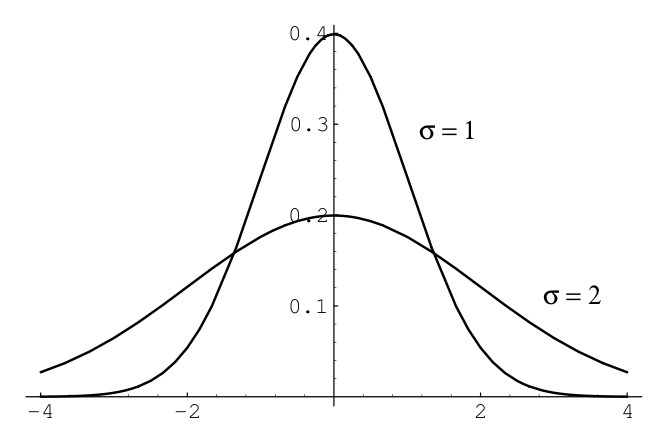
\includegraphics[width=0.6\columnwidth]{figs/intro/normal.png}
  \caption{\label{fig:normaldist} Normal density for two sets of parameter values.}
\end{center}
\end{figure}

Figure \ref{fig:normaldist} compares a plot of normal density for the cases $\mu=0$ and $\sigma=1$, and 
$\mu=0$ and  $\sigma=2$.


\subsection{Maximum Likelihood Estimation}
Until now we assumed that, for every distribution, the parameters $\theta$ are known and are used when we calculate $p(x|\theta)$. There are some cases where the values of the parameters are easy to infer, such as the probability $p$ of getting a head using a fair coin, used on a Bernoulli or Binomial distribution. However, in many problems, these values are complex to define and it is more viable to estimate the parameters using the data $x$. For instance, in the example above with the coin toss, if the coin is somehow tampered to have a biased behavior, rather than examining the dynamics or the structure of the coin to infer a parameter for $p$, a person could simply throw the coin $n$ times, count the number of heads $h$ and set $p=\frac{h}{n}$. By doing so, the person is using the data $x$ to estimate $\theta$.

With this in mind, we will now generalize this process by defining the probability $p(\theta|x)$ as the probability of the parameter $\theta$, given the data $x$. This probability is called {\bf likelihood} $\likelihood(\theta|x)$ and measures how well the parameter $\theta$ models the data $x$. The likelihood can be defined in terms of the distribution $f$ as
\begin{equation*}
\likelihood(\theta|x_1,...,x_n)=\prod_{i=1}^n f(x_i|\theta)
\end{equation*}
where $x_1,...,x_n$ are independently and identically distributed (i.i.d.) samples.

To understand this concept better, we go back to the tampered coin example again. Suppose that we throw the coin 5 times and get the sequence [1,1,1,1,1] (1=head, 0=tail). Using the Bernoulli distribution (see Section~\ref{bernoulli-eq}) $f$ to model this problem, we get the following likelihood values:
\begin{itemize}
\item $\likelihood(0,x) = f(1,0)^5 = 0^5 = 0$
\item $\likelihood(0.2,x) = f(1,0.2)^5 = 0.2^5 = 0.00032$
\item $\likelihood(0.4,x) = f(1,0.4)^5 = 0.4^5 = 0.01024$
\item $\likelihood(0.6,x) = f(1,0.6)^5 = 0.6^5 = 0.07776$
\item $\likelihood(0.8,x) = f(1,0.8)^5 = 0.8^5 = 0.32768$
\item $\likelihood(1,x) = f(1,1)^5 = 1^5 = 1$
\end{itemize}

If we get the sequence [1,0,1,1,0] instead, the likelihood values would be:
\begin{itemize}
\item $\likelihood(0,x) = f(1,0)^3f(0,0)^2 = 0^3\times 1^2 = 0$
\item $\likelihood(0.2,x) = f(1,0.2)^3f(0,0.2)^2 = 0.2^3\times 0.8^2 = 0.00512$
\item $\likelihood(0.4,x) = f(1,0.4)^3f(0,0.4)^2 = 0.4^3\times 0.6^2 = 0.02304$
\item $\likelihood(0.6,x) = f(1,0.6)^3f(0,0.6)^2 = 0.6^3\times 0.4^2 = 0.03456$
\item $\likelihood(0.8,x) = f(1,0.8)^3f(0,0.8)^2 = 0.8^3\times 0.2^2 = 0.02048$
\item $\likelihood(1,x) = f(1,1)^5 = 1^3\times 0^2 = 0$
\end{itemize}

We can see that the likelihood is the highest when the distribution $f$ with parameter $p$ is the best fit for the observed samples. Thus, the best estimate for $p$ according to $x$ would be the value for which $\likelihood(p,x)$ is the highest. 

The value of the parameter $\theta$ with the highest likelihood is called {\bf maximum likelihood estimate (MLE)} and is defined as
\begin{equation*}
\hat{\theta}_{mle}=argmax_{\theta}\likelihood(\theta|x)
\end{equation*}

Finding this for our example is relatively easy, since we can simply derivate the likelihood function to find the absolute maximum. For the sequence [1,0,1,1,0], the likelihood would be given as
\begin{equation*}
\likelihood(p,x) = f(1,p)^3f(0,p)^2 = p^3(1-p)^2
\end{equation*}

And the MLE estimate would be given by:
\begin{equation*}
\frac{\delta \likelihood(p,x)}{\delta p}=0
\end{equation*}
which resolves to
\begin{equation*}
p_{mle}=0.6
\end{equation*}

\begin{exercise}
Over the next couple of exercises we will make use of the Galton dataset, a dataset of heights of fathers and sons from the 1877 paper that first discussed the ``regression to the mean'' phenomenon. This dataset has 928 pairs of numbers.
\begin{itemize}
\item Use the \texttt{load()} function in the \texttt{galton.py} file to load the dataset. The file is located under the \texttt{lxmls/readers} folder. Type the following in your Python interpreter:
\begin{verbatim}
import galton as galton
GaltonData = galton.load()
\end{verbatim}
\item What are the mean height and standard deviation of all the people in the sample? What is the mean height of the fathers and of the sons?
\item Plot a histogram of all the heights (you might want to use the \texttt{plt.hist} function and the \texttt{ravel} method on arrays).
\item Plot the height of the father versus the height of the son.
\item You should notice that there are several points that are exactly the same (e.g., there are 21 pairs with the values 68.5 and 70.2). Use the \texttt{?} command in ipython to read the documentation for the \texttt{numpy.random.randn} function and add random jitter (i.e., move the point a little bit) to the points before displaying them. Does your impression of the data change?
\end{itemize}
\end{exercise}

\subsection{Conjugate Priors}
%\fbox
%{\begin{minipage}[h]{0.9\linewidth} 
\begin{definition}
let $\mathcal{F}= \{f_{X}(x|s), s \in \mathcal{X}\}$ be a class of likelihood functions; let $\mathcal{P}$ be a class of probability (density or mass) functions; if, for any $x$, any $p_{S}(s) \in \mathcal{P}$, and any $f_{X}(x|s) \in \mathcal{F}$, the resulting a posteriori probability function $p_{S}(s|x) = f_{X}(x|s)p_{S}(s)$ is still in $\mathcal{P}$, then $\mathcal{P}$ is called a conjugate family, or a family of {\bf conjugate priors}, for $\mathcal{F}$.
\end{definition}
%\end{minipage}}
%\gka{An example here for conjugate families}


\section{Numerical optimization\label{numerical_optimization}}
Most problems in machine learning require minimization/maximization of functions (likelihoods, risk, energy, entropy, etc.,). Let $x^*$ be the value of $x$ which minimizes the value of some function $f(x)$. Mathematically, this is written as

\begin{equation*}
x^* = \argmin_x f(x)
\end{equation*}

In a few special cases, we can solve this minimization problem analytically in closed form (solving for optimal $x^{*}$ in  $\nabla_{x}f(x^{*})=0$), but in most cases it is too cumbersome (or impossible) to solve these equations analytically, and they must be tackled numerically. In this section we will cover some basic notions of numerical optimization. The goal is to provide the intuitions behind the methods that will be used in the rest of the school. There are plenty of good textbooks in the subject that you can consult for more information \citep{Nocedal1999,bertsekas1995np,boyd2004convex}.

The most common way to solve the problems when no closed form solution is available is to resort to an iterative algorithm. In this Section, we will see some of these iterative optimization techniques. These iterative algorithms construct a sequence of points $x^{(0)},x^{(1)},\ldots \in \text{domain}(f)$ such that hopefully $x^t = x^*$ after a number of iterations.
Such a sequence is called the {\bf minimizing sequence} for the problem.

\subsection{Convex Functions}

One important property of a function $f(x)$ is whether it is a \textbf{convex function} (in the shape of a bowl) or a \textbf{non-convex function}. Figures \ref{fig:convexfn} and \ref{fig:nonconvexfn} show an example of a convex and a non-convex function. Convex functions are particularly useful since you can guarantee that the minimizing sequence converges to the true global minimum of the function, while in non-convex functions you can only guarantee that it will reach a local minimum. 


 \begin{figure}[h]
 \begin{center}
     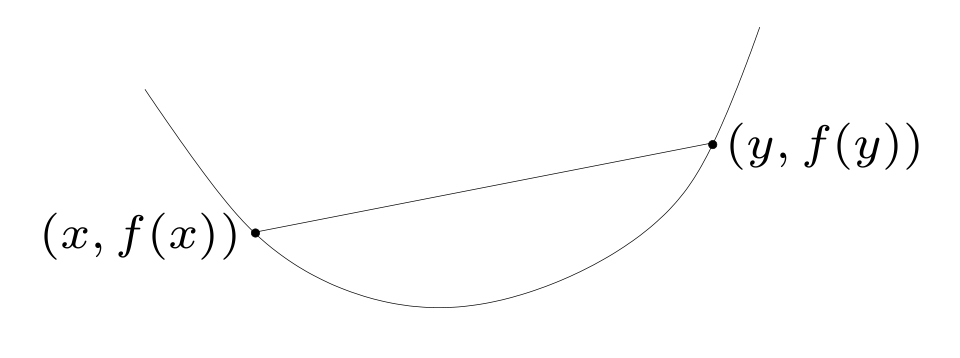
\includegraphics[width=0.6\columnwidth]{figs/intro/convexfn.png}
   \caption{\label{fig:convexfn} Illustration of a convex function. The line segment between any two points on the graph lies entirely above the curve.} 
     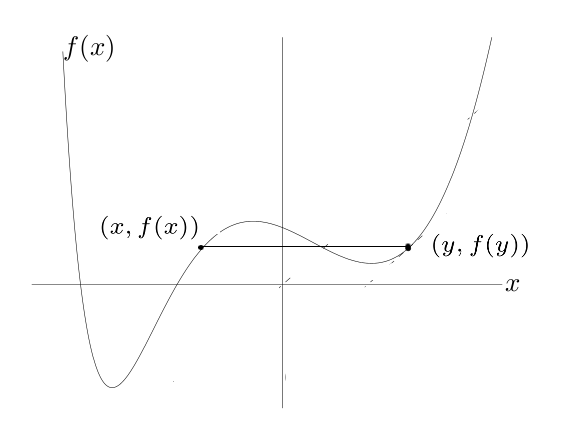
\includegraphics[width=0.5\columnwidth]{figs/intro/nonconvexfn.png}
   \caption{\label{fig:nonconvexfn} Illustration of a non-convex function. Note the line segment intersecting the curve. } 
 \end{center}
 \end{figure}


Intuitively, imagine dropping a ball on either side of Figure \ref{fig:convexfn}, the ball will roll to the bottom of the bowl independently from where it is dropped. This is the main benefit of a convex function. On the other hand, if you drop a ball from the left side of Figure \ref{fig:nonconvexfn} it will reach a different position than if you drop a ball from its right side. Moreover, dropping it from the left side will lead you to a much better (\emph{i.e.}, lower) place than if you drop the ball from the right side. This is the main problem with non-convex functions: there are no guarantees about the quality of the local minimum you find.

More formally, some concepts to understand about convex functions are:

\noindent A {\bf line segment} between points $x_{1}$ and $x_{2}$: contains all points such that 
\begin{equation*}
x=\theta x_{1} + (1-\theta)x_{2}
\end{equation*}
where $0\leq \theta \leq 1$.

\vspace{0.1in}
\noindent A {\bf convex set} contains the line segment between any two points in the set 
\begin{equation*}
x_{1}, x_{2} \in C,\hspace{0.12in} 0 \leq \theta \leq 1 \hspace{0.12in} \Rightarrow \hspace{0.12in} \theta x_{1} + (1-\theta)x_{2} \in C.
\end{equation*}

\vspace{0.1in}
\noindent A function $f: \mathbb{R}^{n}\rightarrow R$ is a {\bf convex function} if the domain of $f$ is a convex set and 
\begin{equation*}
f(\theta x + (1-\theta) y) \leq \theta f(x) + (1-\theta) f(y)
\end{equation*}

\noindent for all $x,y \in \text{domain of } f$, $0 \leq \theta \leq 1$

\subsection{Derivative and Gradient}

The \textbf{derivative} of a function is a measure of how the function varies with its input variables. Given an interval $[a,b]$ one can compute how the function varies within that interval by calculating the average slope of the function in that interval: 
\begin{equation}
\frac{f(b) - f(a)}{b-a}.
\end{equation}
The derivative can be seen as the limit as the interval goes to zero, and it gives us the slope of the function at that point.
\begin{equation}
\frac {\partial f}{\partial x} = \lim_{h = 0} \frac{f(x+h) - f(x)}{h} 
\end{equation}

\noindent Table \ref{tb::derivatives} shows derivatives of some functions that we will be using during the school.

\begin{table}[!h]
\begin{center}
\begin{tabular}{|l|l|}
\hline
Function $f(x)$& Derivative $\frac{\partial f}{\partial x}$\\
\hline
$x^2$ & $2x$\\
\hline
$x^n$ & $nx^{n-1}$\\
\hline
$\log(x)$ & $\frac{1}{x}$\\
\hline
$\exp(x)$ & $\exp(x)$\\
\hline
$\frac{1}{x}$ & $-\frac{1}{x^{2}}$\\
\hline
\end{tabular}
\end{center}
\caption{\label{tb::derivatives}Some derivative examples}
\end{table}

An important rule of derivation is the chain rule. Consider $h=f\circ g$, and $u=g(x)$, then:

\begin{equation}
\frac{\partial h}{\partial x}=\frac{\partial f}{\partial u}\cdot\frac{\partial g}{\partial x}
\end{equation}

\begin{example}

Consider the function $h(x)=\exp(x^{2})$, this can be decomposed as $h(x)=f(g(x))=f(u)=\exp(u)$, where $u=g(x)=x^{2}$ and has derivative $\frac{\partial h}{\partial x}=\frac{\partial f}{\partial u}\cdot \frac{\partial u}{\partial x}=\exp(u) \cdot 2x=\exp(x^{2}) \cdot 2x$

\end{example}

\begin{exercise}
Consider the function $f(x) = x^2$ and its derivative $\frac{\partial f} {\partial x}$. Look at the derivative of that function at points [-2,0,2], draw the tangent to the graph in that point $\frac{\partial f}{\partial x}\left(-2\right)=-4$, $\frac{\partial f}{\partial x}\left(0\right)=0$, and $\frac{\partial f}{\partial x}\left(2\right)=4$. For example, the tangent equation for $x=-2$ is $y=-4x - b$, where $b=f(-2)$. The following code plots the function and the derivatives on those points using matplotlib (See Figure \ref{fig:tangents}).

\begin{python}
a = np.arange(-5,5,0.01)
f_x = np.power(a,2)
plt.plot(a,f_x)

plt.xlim(-5,5)
plt.ylim(-5,15)

k= np.array([-2,0,2])
plt.plot(k,k**2,"bo")
for i in k:
    plt.plot(a, (2*i)*a - (i**2))

\end{python}

\begin{figure}[h]
\begin{center}
   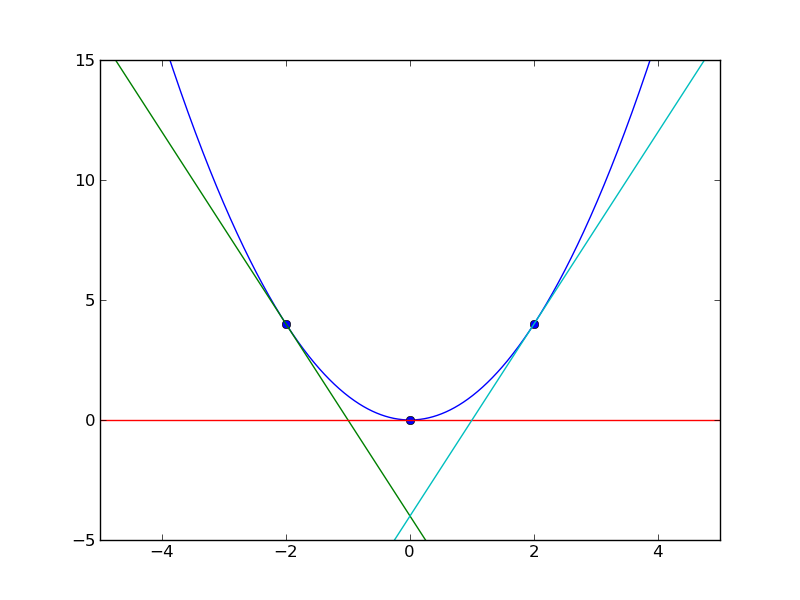
\includegraphics[width=0.6\columnwidth]{figs/intro/tangents.png}
 \caption{\label{fig:tangents} Illustration of the gradient of the
   function $f(x^2)$ at three different points $x = [-2,0.2]$. Note
   that at point $x = 0$ the gradient is zero which corresponds to the
 minimum of the function.}
\end{center}
\end{figure}

\end{exercise}

The \textbf{gradient} of a function is a generalization of the derivative concept we just saw before for several dimensions. Lets assume we have a function  $f(x)$ where $x \in \mathbb{R}^2$, so $x$ can be seen as a pair $x = [{x_1,x_2}]$. Then, the gradient measures the slope of the function in both directions: $\nabla_{x} f(x) = [\frac {\partial f}{\partial x_1},\frac {\partial f}{\partial x_2}]$.

\subsection{\label{gradient_methods} Gradient Based Methods}

Gradient based methods are probably the most common methods used for finding the minimizing sequence for a given function. The methods used in this class will make use of the function value $f(x)$ as well as the gradient of the function $\nabla_{x} f(x)$. The simplest method is the {\bf Gradient descent} method, an unconstrained first-order optimization algorithm.

The intuition of this method is as follows: You start at a given point $x_0$ and compute the gradient at that point $\nabla_{x_0} f(x)$. You then take a step of length $\eta$ on the direction of the negative gradient to find a new point: $x_1$ = $x_0 - \eta \nabla_{x_{0}}
f(x)$. Then, you compute the gradient at this new point, $\nabla_{x_1} f(x)$, and take a step of length $\eta$ on the direction of the negative gradient to find a new point: $x_2$ = $x_1 - \eta \nabla_{x_{1}} f(x)$. You proceed until you have reached a minimum (local or global). Recall from the previous subsection that you can identify the minimum by testing if the norm of the gradient is zero: $||\nabla f(x)|| = 0$.

There are several practical concerns even with this basic algorithm to ensure both that the algorithm converges (reaches the minimum) and that it does so in a fast way (by fast we mean the number of function and gradient evaluations).

\begin{itemize}
\item \textbf{Step Size $\eta$} A first question is how to find the step length $\eta$. One condition is that $eta$ should guarantee sufficient decrease in the function value. We will not cover these methods here but the most common ones are \textbf{Backtracking line search} or the \textbf{Wolf Line Search} \citep{Nocedal1999}.
\item \textbf{Descent Direction}  A second problem is that using the negative gradient as direction can lead to a very slow convergence. Different methods that change the descent direction by multiplying the gradient by a matrix $\beta$ have been proposed that guarantee a faster convergence. Two notable methods are the Conjugate Gradient (CG) and the Limited Memory Quasi Newton methods (LBFGS) \citep{Nocedal1999}.
\item \textbf{Stopping Criteria} Finally, it will normally not be possible to reach full convergence either because it will be too slow, or because of numerical issues (computers cannot perform exact arithmetic). So normally we need to define a stopping criteria for the algorithm. Three common criteria (that are normally used together) are: a maximum number of iterations; the gradient norm be smaller than a given threshold   $||\nabla f(x)|| \leq \eta_1$, or the normalized difference in the function value be smaller than a given threshold $\frac{|f(x_t) - f(x_{t-1})|}{\max(|f(x_t)|,|f(x_{t-1})|)} \leq \eta_2$
\end{itemize}

Algorithm \ref{alg:graddescent} shows the general gradient based algorithm. Note that for the simple gradient descent algorithm $\beta$ is the identity matrix and the descent direction is just the negative gradient of the function, $\beta = -\nabla f(x)$. Figure \ref{fig:graddescent} shows an illustration of the gradient descent algorithm.

\begin{algorithm}[h]
\caption{Gradient Descent\label{alg:graddescent}}
\begin{algorithmic}[1]
\STATE {\bf given} a starting point $x_{0}, i=0$
\STATE {\bf repeat}
\STATE \quad Compute step size $\eta$
\STATE \quad Compute descent direction $- \beta\nabla f(x_{i})$.
\STATE \quad $x_{i+1} \leftarrow x_{i} - \eta\beta\nabla f(x_{i})$
\STATE \quad $i \leftarrow i + 1$
\STATE {\bf until} stopping criterion is satisfied.
\end{algorithmic}
\end{algorithm}

\begin{figure}[h]
\begin{center}
   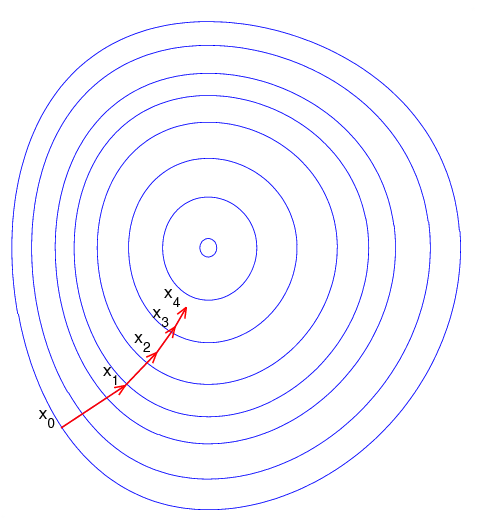
\includegraphics[width=0.6\columnwidth]{figs/intro/graddescent.png}
 \caption{\label{fig:graddescent} Illustration of gradient descent. The blue circles correspond to contours of the function (each blue circle is a set of points which have the same function value), while the red lines correspond to steps taken in the negative gradient direction.}
\end{center}
\end{figure}

% Gradient descent can work in any number of dimensions.  The process can also include {\bf line search} 
% to determine the locally optimal $\eta$ in each iteration. For non-differentiable functions, gradient 
% methods are ill-defined. Also, the procedure can take many iterations to converge to a local minimum 
% and methods based on Newton's method can be better alternatives. The main idea behind
% the iterative minimization techniques is find the locally best direction to move towards the (unknown) minimum. 
% While gradient descent moves in the direction of the negative gradient, other techniques like steepest 
% descent, conjugate descent, (L-)BGFS etc use other directions for update.

\begin{exercise}
Consider the function $f(x) = (x+2)^2 - 16 \exp\left( -(x-2)^2 \right)$.
Make a function that computes the function value given $x$.

\begin{python}
def get_y(x):
    return (x+2)**2 - 16*np.exp(-((x-2)**2))
\end{python}

Draw a plot around $x \in [-8,8]$.

\begin{python}
x = np.arange(-8,8,0.001)
y = map(lambda u: get_y(u),x)
plt.plot(x,y)
plt.show()
\end{python}

Calculate the derivative of the function $f(x)$, implement the function \emph{get\_grad(x)}.

\begin{python}
def get_grad(x):
    return (2*x+4)-16*(-2*x + 4)*np.exp(-((x-2)**2))
\end{python}

Use the method \emph{gradient\_descent} to find the minimum of this function. Convince yourself that the code is doing the proper thing. Look at the constants we defined. Note, that we are using a simple approach to pick the step size (always have the value step\_size) which is not necessarily correct.

\begin{python}
def gradient_descent(start_x,func,grad):
    # Precision of the solution
    prec = 0.0001
    #Use a fixed small step size
    step_size = 0.1
    #max iterations
    max_iter = 100
    x_new = start_x
    res = []
    for i in xrange(max_iter):
        x_old = x_new
        #Use beta egual to -1 for gradient descent 
        x_new = x_old - step_size * grad(x_new)
        f_x_new = func(x_new)
        f_x_old = func(x_old)
        res.append([x_new,f_x_new])
        if(abs(f_x_new - f_x_old) < prec):
            print "change in function values too small, leaving"
            return np.array(res)
    print "exceeded maximum number of iterations, leaving"
    return np.array(res)
\end{python}

Run the gradient descent algorithm starting from $x_0 = -8$ and plot the minimizing sequence.

\begin{python}
x_0 = -8
res = gradient_descent(x_0,get_y,get_grad)
plt.plot(res[:,0],res[:,1],'+')
plt.show()
\end{python}


\begin{figure}[h]
\begin{center}
   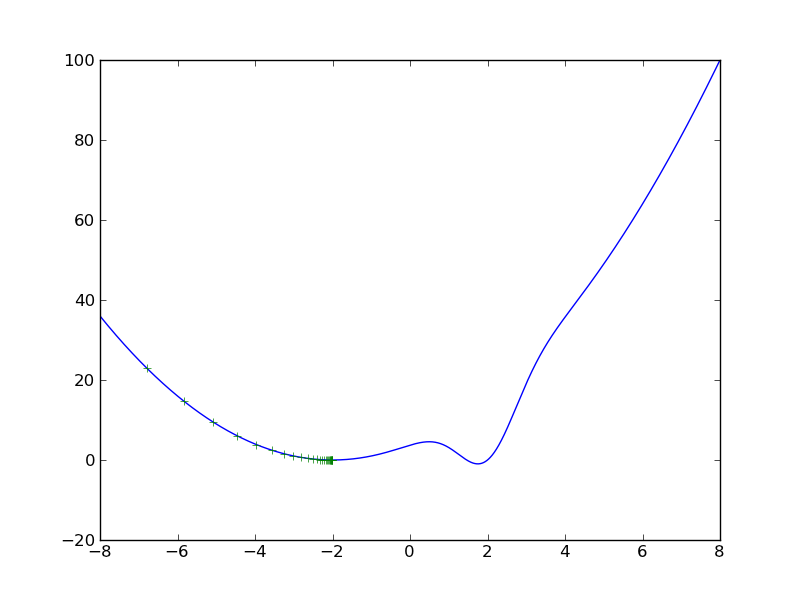
\includegraphics[width=1\columnwidth]{figs/intro/gradex1.png}
 \caption{\label{fig:gradex1} Example of running gradient descent
   starting on point $x_0 = -8$ for function $f(x) = (x+2)^2 - 16
   \exp\left( -(x-2)^2 \right)$. The function is represented in blue,
   while the points of the minimizing sequence are displayed as green
   plus signs.}
\end{center}
\end{figure}


Figure \ref{fig:gradex1} shows the resulting minimizing sequence. Note that the algorithm converged to a minimum, but since the function is not convex it converged only to a local minimum.

Now try the same exercise starting from the initial point $x_0 = 8$.

\begin{python}
x_0 = 8
res = gradient_descent(x_0,get_y,get_grad)
plot(res[:,0],res[:,1],'+')
\end{python}


\begin{figure}[h]
\begin{center}
   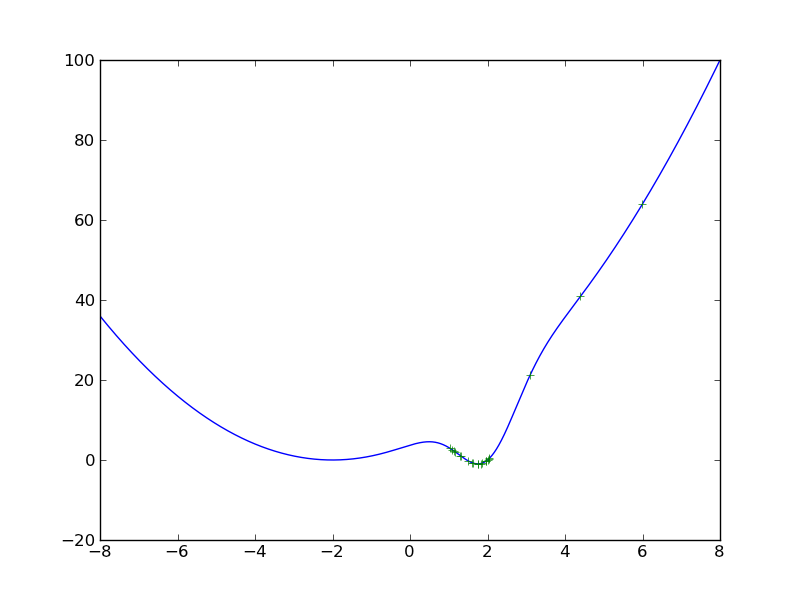
\includegraphics[width=1\columnwidth]{figs/intro/gradex2.png}
 \caption{\label{fig:gradex2} Example of running gradient descent
   starting on point $x_0 = 8$ for function $f(x) = (x+2)^2 - 16
   \exp\left( -(x-2)^2 \right)$. The function is represented in blue,
   while the points of the minimizing sequence are displayed as green
   plus signs.}
\end{center}
\end{figure}


Figure \ref{fig:gradex2} shows the resulting minimizing sequence. Note that now the algorithm converged to the global minimum. However, note that to get to the global minimum the sequence of points jumped from one side of the minimum to the other. This is a consequence of using a wrong step size (in this case too large). Repeat the previous exercise changing both the values of the step-size and the precision. What do you observe?
\end{exercise}

During this school we will rely on the numerical optimization methods provided by Scipy (scientific computing library in python), which are very efficient implementations.


% \begin{exercise}
% Consider the linear regression problem (ordinary least squares), with a
% single response variable

% \[
% y = x^T w + \varepsilon
% \]

% The \emph{linear regression problem} is, given a set $\{ y^{(i)} \}_i$ of
% samples of $y$ and the corresponding $\vect{x}^{(i)}$ vectors, estimate
% $\vect{w}$ to minimise the sum of the $\varepsilon$ variables. Traditionally
% this is solved analytically to obtain a closed form solution (although this is
% \textbf{not the way in which it should be computed}, linear algebra packages
% have an optimised solver, with numpy, use \code{numpy.linalg.lstsq}).

% Alternatively, we can define the error function for each possible $\vect{w}$:

% \[
% e(\vect{w}) = \sum_i \left( {\vect{x}^{(i)}}^T \vect{w} - y^{(i)} \right)^2.
% \]

% \begin{enumerate}
% \item Derive the gradient of the error $\pd{e}{w_j}$.
% \item Implement a solver based on this for two dimensional problems (i.e.,
% $\vect{w} \in R^2$).
% \item Use this method on the Galton dataset from the previous exercise to
% estimate the relationship between father and son's height. Try two formulas
% \begin{equation}
% s = f w_1 + \varepsilon,
% \label{}
% \end{equation}
% where $s$ is the son's height, and $f$ is the father heights; and
% \begin{equation}
% s = f w_1 + 1w_0 + \varepsilon
% \label{}
% \end{equation}
% where the input variable is now two dimensional: $(f,1)$. This allows the
% intercept to be non-zero.
% \item Plot the regression line you obtain with the points from the previous
% exercise.
% \item Use the \texttt{np.linalg.lstsq} function and compare to your solution.
% \end{enumerate}
% \end{exercise}



%Basic concepts of numerical optimization.

%\begin{itemize}
%\item - Gradient base methods, gradient descent, its problems,
%  conjugate and lbfgs. Can use routines from python, make example with
%  Gaussian with different variates and show the behavior.
%\item convex functions vs non convex functions, very brief, convex
%  function is like a bowl, if you drop a ball from the top it will
%  reach the bottom, Non-convex several bottom, will reach one of them.
%\item Gradient, sub-gradient generalization
%\end{itemize}


% \subsection{Matrix Derivatives}

% In subsection we finalize by showing some basic formulas for the
% gradient of matrix:

% \begin{itemize}
% \item For vectors $a$ and $x$, $\frac{\partial a^{T} x}{\partial x}= a$
% \item For vectors $a$ and $x$ and matrix $A$, $\frac{\partial a^{T}Ab}{\partial A} = ab^{T}$
% \item For vectors $a$ and $x$ and matrix $A$, $\frac{\partial a^{T}A^{T}b}{\partial A} =  ba^{T}$
% \end{itemize}

% {\bf The Gradient: }Suppose that $f:\mathbb{R}^{m\times n} \rightarrow\mathbb{R}$ is a function that takes as input, a matrix $A$
% of size $m\times n$ and returns a real value. Then the {\bf gradient} of $f$ (with respect to $A\in \mathbb{R}^{m\times n}$)
% is the matrix of partial derivatives, defined as:
% \begin{equation*}
% \nabla_{A}f(A)\in \mathbb{R}^{m\times n} = \left[\begin{array}{cccc}
% \frac{\partial f(A)}{\partial A_{11}} & \frac{\partial f(A)}{\partial A_{12}} & \ldots & \frac{\partial f(A)}{\partial A_{1n}} \\
% \frac{\partial f(A)}{\partial A_{21}} & \frac{\partial f(A)}{\partial A_{22}} & \ldots & \frac{\partial f(A)}{\partial A_{2n}} \\
% \vdots & \vdots &\ddots & \vdots \\
% \frac{\partial f(A)}{\partial A_{m1}} & \frac{\partial f(A)}{\partial A_{m2}} & \ldots & \frac{\partial f(A)}{\partial A_{mn}} \\
% \end{array}\right].
% \end{equation*}

% The gradient is defined {\em only} if the function is real-valued, that is, if it returns a scalar value. Some 
% important properties:

% \begin{itemize}
% \item $\nabla_{x}(f(x) + g(x)) = \nabla_{x}f(x) + \nabla_{x}g(x)$.
% \item For $t \in \mathbb{R}$, $\nabla_{x}(tf(x))= t\nabla_{x}f(x)$.
% \item Let $f:\mathbb{R}^{m} \rightarrow \mathbb{R}$ be the function defined by $f(z)=z^{T}z$, $\nabla_{z}f(z)=2z$.
% \end{itemize}
% {\bf The Hessian:} Suppose that $f:\mathbb{R}^{n}\rightarrow\mathbb{R}$ is a function that takes a vector in $\mathbb{R}^{n}$ and
% returns a real number, then the {\em Hessian} matrix with respect to $x$, written $\nabla_{x}^{2}f(x)$ (or $H$) is the $n\times n$
% matrix of partial derivatives,

% \begin{equation*}
% \nabla_{x}^{2}f(x) \in \mathbb{R}^{n\times n}= \left[\begin{array}{cccc}
% \frac{\partial^{2}f(x)}{\partial x_{1}^{2}} & \frac{\partial^{2}f(x)}{\partial x_{1} \partial x_{2}} & \ldots &  \frac{\partial^{2}f(x)}{\partial x_{1} \partial x_{n}} \\
% \frac{\partial^{2}f(x)}{\partial x_{2} \partial x_{1}} & \frac{\partial^{2}f(x)}{\partial x_{2}^{2}} & \ldots &  \frac{\partial^{2}f(x)}{\partial x_{2} \partial x_{n}} \\
% \vdots & \vdots & \ddots & \vdots \\
% \frac{\partial^{2}f(x)}{\partial x_{n} \partial x_{1}} & \frac{\partial^{2}f(x)}{\partial x_{n}\partial x_{2}} & \ldots &  \frac{\partial^{2}f(x)}{\partial x_{n}^{2}} 

% \end{array}\right].
% \end{equation*}

% Note that the Hessian is always symmetric, since
% \begin{equation*}
% \frac{\partial^{2}f(x)}{\partial x_{i}\partial x_{j}} =\frac{\partial^{2}f(x)}{\partial x_{j}\partial x_{i}}.
% \end{equation*}



%%% Local Variables: 
%%% mode: latex
%%% TeX-master: "../../guide"
%%% End: 


\section{Python Exercises}




\subsection{Numpy and Matplotlib}

%As discussed in the lecture, there are many helpful functions in numpy. For basic mathematical operations, we have \code{np.log}, \code{np.exp}, \code{np.cos},\ldots with the expected meaning. These operate both on single arguments and on arrays (where they will behave element wise).

%\begin{python}
%import matplotlib.pyplot as plt
%import numpy as np
%X = np.linspace(0, 4 * np.pi, 1000)
%C = np.cos(X)
%S = np.sin(X)

%plt.plot(X, C)
%plt.plot(X, S)
%\end{python}

%Other functions take a whole array and compute a single value from it. For
%example, \code{np.sum}, \code{np.mean},\ldots These are available as both free
%functions and as methods on arrays.

%\begin{python}
%import numpy as np
%A = np.arange(100)
%print np.mean(A)
%print A.mean()

%C = np.cos(A)
%print C.ptp()
%\end{python}

%\begin{exercise}
%Run the above example and lookup the \code{ptp} function/method.
%\end{exercise}

%\begin{exercise}
%Consider the following approximation to compute an integral

%\[
%\int_0^{1} f(x)dx \approx \sum_{i = 0}^{999} \frac{f(i/1000)}{1000}.
%\]

%Use numpy to implement this for $f(x) = x^2$. You should not need to use any
%loops.
%\end{exercise}

%\begin{exercise}
%\begin{enumerate}
%\item Consider the function $f(x) = (x+2)^2 - 16 \exp\left( -(x-2)^2 \right)$.
%Draw a plot around the $x \in [-8,8]$ region.
%\item What is $\pd{f}{x}$?
%\item Use gradient descent to find a local minimum starting from $x_0 = -4$ and
%$x_0 = +4$, with $\eta = .01$. Plot all of the intermediate estimates that you
%obtain in the same plot.
%\end{enumerate}
%\begin{python}
%import numpy as np
%import matplotlib.pyplot as plt
%X = np.linspace(-8, 8, 1000)
%Y = (X+2)**2 - 16*np.exp(-((X-2)**2))
%
%# derivative of the function f
%def get_Y_dev(x):
%    return (2*x+4)-16*(-2*x + 4)*np.exp(-((x-2)**2))
%
%def grad_desc(start_x, eps, prec):
%    '''
%    runs the gradient descent algorithm and returns the list of estimates
%
%    example of use grad_desc(start_x=3.9, eps=0.01, prec=0.00001)
%    '''
%    x_new = start_x
%    x_old = start_x + prec * 2
%    res = [x_new]
%    while abs(x_old-x_new) > prec:
%        x_old = x_new
%        x_new = x_old - eps * get_Y_dev(x_new)
%        res.append(x_new)
%    return np.array(res)
%\end{python}
%\end{exercise}

%Over the next couple of exercises we will make use of the Galton dataset, a
%dataset of heights of fathers and sons from the 1877 paper that first discussed
%the ``regression to the mean'' phenomenon.
%
%\begin{exercise}
%\begin{itemize}
%\item Use the \texttt{load()} function in the \texttt{galton.py} file to load
%the dataset.
%\item What are the mean height and standard deviation of all the people in the
%sample? What is the mean height of the fathers and of the sons?
%\item Plot a histogram of all the heights (you might want to use the
%\texttt{plt.hist} function and the \texttt{ravel} method on arrays).
%\item Plot the height of the father versus the height of the son.
%\item You should notice that there are several points that are exactly the same
%(e.g., there are 21 pairs with the values 68.5 and 70.2). Use the \texttt{?}
%command in ipython to read the documentation for the \texttt{numpy.random.rand}
%function and add random jitter (i.e., move the point a little bit) to the
%points before displaying them. Does your impression of the data change?
%\end{itemize}
%\end{exercise}

\begin{exercise}
Consider the linear regression problem (ordinary least squares) on the Galton
dataset, with a single response variable

\[
y = x^T w + \varepsilon
\].

The \emph{linear regression problem} is, given a set $\{ y^{(i)} \}_i$ of
samples of $y$ and the corresponding $\vect{x}^{(i)}$ vectors, estimate
$\vect{w}$ to minimise the sum of the $\varepsilon$ variables. Traditionally
this is solved analytically to obtain a closed form solution (although this is
\textbf{not the way in which it should be computed} in this exercise, linear algebra packages
have an optimised solver, with numpy, use \code{numpy.linalg.lstsq}).

Alternatively, we can define the error function for each possible $\vect{w}$:

\[
e(\vect{w}) = \sum_i \left( {\vect{x}^{(i)}}^T \vect{w} - y^{(i)} \right)^2.
\]

\begin{enumerate}
\item Derive the gradient of the error $\pd{e}{w_j}$.
\item Implement a solver based on this for two dimensional problems (i.e.,
$\vect{w} \in R^2$).
\item Use this method on the Galton dataset from the previous exercise to
estimate the relationship between father and son's height. Try two formulas
\begin{equation}
s = f w_1 + \varepsilon,
\label{}
\end{equation}
where $s$ is the son's height, and $f$ is the father heights; and
\begin{equation}
s = f w_1 + 1w_0 + \varepsilon
\label{}
\end{equation}
where the input variable is now two dimensional: $(f,1)$. This allows the
intercept to be non-zero.
\item Plot the regression line you obtain with the points from the previous
exercise.
\item Use the \texttt{np.linalg.lstsq} function and compare to your solution.
\end{enumerate}

Please refer to the notebook for solutions.
\end{exercise}

\subsection{Debugging}


\begin{exercise}
Use the debugger to debug the \texttt{buggy.py} script which attempts to
repeatedly perform the following computation:

\begin{enumerate}
\item Start $x_0 = 0$
\item Iterate

\begin{enumerate}
\item $x'_{t+1} = x_t + r$, where $r$ is a random variable.
\item if $x'_{t+1} >= 1.$, then stop.
\item if $x'_{t+1} <= 0.$, then $x_{t+1} = 0$
\item else $x_{t+1} = x'_{t+1}$.
\end{enumerate}
\item Return the number of iterations.
\end{enumerate}

Having repeated this computation a number of times, the programme prints the
average. Unfortunately, the program has a few bugs, which you need to fix.
\end{exercise}




\chapter{\label{day:classification}Linear Classifiers}

This day will serve as an introduction to machine learning. We recall some fundamental concepts 
about decision theory and classification. We also present some widely used models and algorithms 
and try to provide the main motivation behind them. 
There are several textbooks that provide a thorough description of some of the concepts introduced here: 
for example, \citet{Mitchell1997},\citet{Duda2001}, \citet{Schoelkopf2002}, \citet{Joachims2002}, \citet{Bishop2006}, \citet{Manning2008}, 
to name just a few.  
The concepts that we introduce in this chapter will be revisited in later chapters, where the same algorithms and models 
will be adapted to structured inputs and outputs. For now, we concern only with multi-class classification 
(with just a few classes). 

\section*{Today's assignment}

The assignment of today's class is to implement a classifier called Naive Bayes, and use it to perform sentiment analysis on a corpus of book reviews from Amazon.

\section{Pre-assignment}

\subsection{Notation}

In what follows, we denote by $\mathcal{X}$ our \emph{input set} (also called \emph{observation set}), and by $\mathcal{Y}$ our \emph{output set}. 
We will make no assumptions about the set $\mathcal{X}$, which can be continuous or discrete. In this lecture, we 
consider \emph{classification} problems, where $\mathcal{Y} = \{c_1,\ldots,c_K\}$ is a finite set, consisting of $K$ \emph{classes} (also called \emph{labels}). 
For example, $\mathcal{X}$ can be a set of documents in natural language, and $\mathcal{Y}$ a set of topics, the goal 
being to assign a topic to each document. 

We use upper-case letters for denoting random variables, and lower-case letters for value assignments to those variables:  
for example, 
\begin{itemize}
\item $X$ is a random variable taking values on $\mathcal{X}$,
\item $Y$ is a random variable taking values on $\mathcal{Y}$,
\item $x \in \mathcal{X}$ and $y \in \mathcal{Y}$ are particular values for $X$ and $Y$. 
\end{itemize}  
We consider \emph{events} such as $X=x$, $Y=y$, etc. 
Throughout, we use modified notation and let $P(y)$ denote the \emph{probability} associated with the event $Y=y$ (instead of writing $P_Y(Y=y)$). 
\emph{Joint} and \emph{conditional} probabilities are 
denoted respectively as $P(x,y) \triangleq P_{X,Y}(X=x \wedge Y=y)$ and $P(x|y) \triangleq P_{X|Y}(X=x \,\,|\,\,Y=y)$. From the laws of probabilities: 
\begin{equation}
P(x,y)=P(y|x) P(x) = P(x|y) P(y), 
\end{equation}
for all $x \in \mathcal{X}$ and $y \in \mathcal{Y}$.

Quantities that are predicted or estimated from the data will be appended a hat-symbol: for example, estimations of the probabilities above are denoted 
as ${\hat P}(y)$, ${\hat P}(x,y)$ and ${\hat P}(y|x)$; and a prediction of an output will be denoted ${\hat y}$. 

We assume that a \emph{training dataset} $\mathcal{D}$ is provided
which consists of $M$ input-output pairs (called \emph{examples} or
\emph{instances}): 
\begin{equation}
\mathcal{D} = \{(x^{1},y^{1}),\ldots,(x^{M},y^{M})\} \subseteq \mathcal{X} \times \mathcal{Y}.  
\end{equation}

The goal of (supervised) machine learning is to use the training dataset $\mathcal{D}$ to learn a function $h$ (called a \emph{classifier}) 
that maps from $\mathcal{X}$ to $\mathcal{Y}$: this way, given a new instance 
$x \in \mathcal{X}$ (test example), the machine makes a prediction ${\hat y}$ by evaluating $h$ on $x$, i.e., ${\hat y} = h(x)$. 

%\out{
\begin{figure}
\begin{center}
    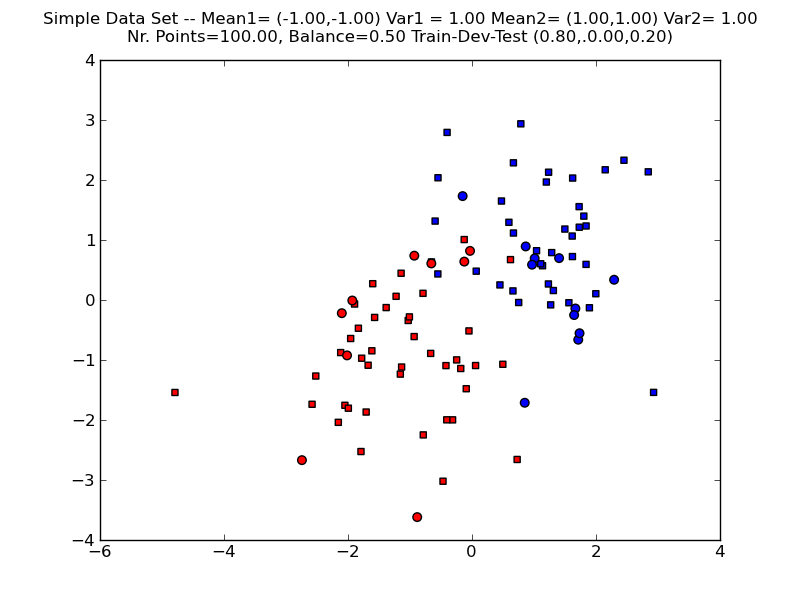
\includegraphics[width=1\columnwidth]{figs/classification/simple_data_set}
  \caption{\label{simpleDataSet} Example of a dataset.
    The input set consists in points in the real plane, $\mathcal{X} =
    \mathbb{R}^2$, and the output set consists of two classes (Red
    and Blue). Training points are represented as squares, while test
    points are represented as circles.}
  \end{center}
\end{figure}
%}

\subsection{\label{s::naiveBayes}Generative Classifiers: Na\"{i}ve Bayes}

If we knew the \emph{true} distribution $P(X,Y)$, the best possible classifier (Bayes optimal) 
would be one which predicts according to

\begin{eqnarray}
{\hat y} &=& \arg\max_{y \in \mathcal{Y}} P(y|x) = \arg\max_{y \in \mathcal{Y}} \frac{P(x,y)}{P(x)} \nonumber\\
&=^{\dagger}& \arg\max_{y \in \mathcal{Y}} P(x,y) \nonumber \\
&=& \arg\max_{y \in \mathcal{Y}} P(y) P(x|y),
\end{eqnarray}
where in ${\dagger}$ we used the fact that $P(x)$ is constant with respect to $y$. Generative classifiers try to estimate the probability distributions $P(Y)$ and $P(X|Y)$ (which are respectively called the \emph{class prior} and the \emph{class conditionals}).
  
Figure \ref{simpleDataSet_bo} shows an example of
the Bayes optimal decision boundary for a toy example with $K=2$ classes, $M=100$ points, class priors $P(y_1) = P(y_2) = 0.5$, and class conditionals $P(x|y_i)$ given by 2-D Gaussian distributions with the same variance but different means.

\begin{figure}[h]
\begin{center}
    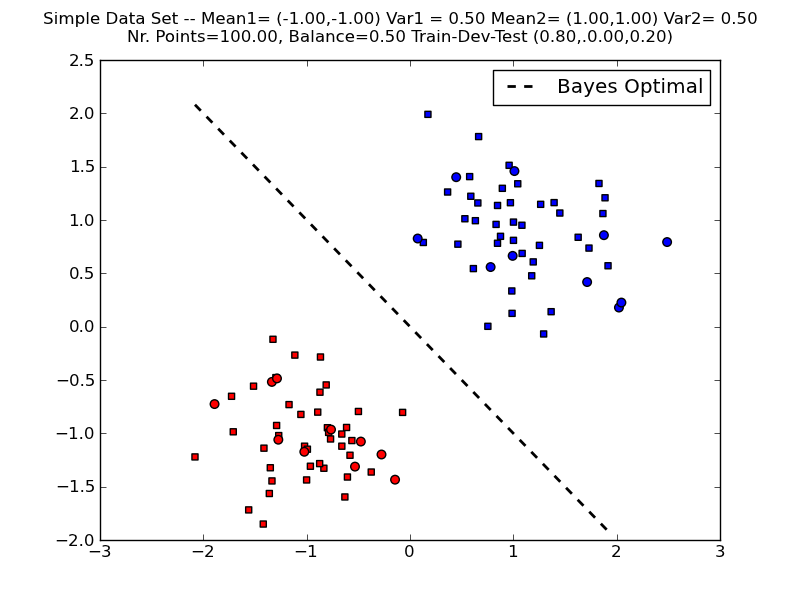
\includegraphics[width=1\columnwidth]{figs/classification/gaussian_separabale_bo.png}
  \caption{\label{simpleDataSet_bo} Example of a dataset together with
    the corresponding Bayes optimal decision boundary.
    The input set consists in points in the real plane, $\mathcal{X} =
    \mathcal{R^2}$, and the output set consists of two classes (Red
    and Blue). Training points are represented as squares, while test
    points are represented as circles.}
  \end{center}
\end{figure}



Generative models assume that the data are generated according to the following generative story (independently for each $m=1,\ldots,M$): 
\begin{enumerate}
\item A class $y_m \sim P(Y)$ is drawn from the class prior distribution;
\item An input $x_m \sim P(X|Y=y_m)$ is drawn from the corresponding class conditional.
\end{enumerate}
Training a generative model 
amounts to \emph{estimating} these probabilities using the dataset $\mathcal{D}$, yielding estimates 
$\hat{P}(y)$ and $\hat{P}(x|y)$. This estimation is usually called \emph{training}, or \emph{learning}.

After we are done training, we are given a new input $x \in \mathcal{X}$, and we want to make a prediction according to  
\begin{eqnarray}
{\hat y} &=& \arg\max_{y \in \mathcal{Y}} \hat{P}(y) \hat{P}(x|y),
\label{eq:argmax}
\end{eqnarray}
using the probabilities estimated in the training stage. This is usually called \emph{inference} or \emph{decoding}.


We are left with two important problems:
\begin{enumerate}
\item How should the distributions ${\hat P}(Y)$ and ${\hat P}(X|Y)$ be ``defined''?
(i.e., what kind of independence assumptions should they state, or how should they factor?)
\item How should parameters be estimated from the training data $\mathcal{D}$?
\end{enumerate}

The first problem strongly depends on the application at hand. Quite often, there is a natural decomposition of the input variable $X$ into $J$ components, 
\begin{equation}
X = (X_1,\ldots,X_J). 
\end{equation}
The na\"{i}ve Bayes method makes the following assumption: \emph{$X_1,\ldots,X_J$ are conditionally independent given the class}. Mathematically, this means that 
\begin{eqnarray}
P(X|Y) &=& \prod_{j=1}^J P(X_j|Y).
\end{eqnarray}
Note that this independence assumption greatly reduces the number of parameters to be estimated (degrees of freedom) 
from $O(\exp(J))$ to $O(J)$, 
hence estimation of ${\hat P}(X|Y)$ becomes much simpler, as we shall see. 
It also makes the overall computation much more efficient for large $J$ and it decreases the risk of overfitting the data. 
On the other hand, if the assumption is over-simplistic it may increase the risk 
of under-fitting. 
%This choice greatly simplifies the problem of parametrizing ${\hat P}(Y)$ and ${\hat P}(X|Y)$. 

For the second problem, one of the simplest ways to solve it is using \emph{maximum likelihood estimation}, which aims to maximize the probability of the training sample, assuming that each point was generated independently. This probability (call it $P(\mathcal{D})$) factorizes as 
\begin{eqnarray}
P(\mathcal{D}) &=& \prod_{m=1}^M P(x^m,y^m) \nonumber\\
&=& \prod_{m=1}^M P(y^m)\prod_{j=1}^J P(x^m_j|y^m). 
\end{eqnarray}



%%\begin{example}[2-D Gaussians] 
%\subsection{Example: 2-D Gaussians}
%
%We first illustrate the na\"ive Bayes assumption with a toy example. 
%Suppose that $\mathcal{X}=\mathbb{R}^2$ and $\mathcal{Y}=\{1,2\}$. 
%Assume that each class-conditional is a two-dimensional Gaussian distribution with fixed covariance, 
%i.e., $P(X_1,X_2|Y=y)=\mathcal{N}(\boldsymbol{\mu}_y, \boldsymbol{\Sigma}_y)$. 
%
%According to the na\"ive Bayes assumption, ${\hat P}(X_1,X_2|Y) = {\hat P}(X_1|Y) {\hat P}(X_2|Y)$ (remark: this 
%is equivalent to assuming that 
%the $\boldsymbol{\Sigma}_y$ are diagonal!). For simplicity, we also assume that the two classes have unit variance. Then, we have 
%${\hat P}(X_1|Y=y) = \mathcal{N}(\mu_{y1}, 1.0)$ 
%and ${\hat P}(X_2|Y=y) = \mathcal{N}(\mu_{y2}, 1.0)$. Figure
%\ref{simpleDataSet} shows an example a dataset of two gaussians with unit
%variance, where $\mu_{y1} = [-1,-1]$ and $\mu_{y1} = [1,1]$. Figure
%\ref{simpleDataSet_bo} shows the same example but where both
%gaussians have $\Sigma = 0.5$, together with the Bayes optimal decision boundary. 
%The parameters that need to be estimated are the class-conditional means $\mu_{11},\mu_{12},\mu_{21},\mu_{22}$ and 
%the class priors ${\hat P}(Y=1)$ and ${\hat P}(Y=2)$. Given a training sample $\mathcal{D} = \{(x^{1},y^{1}),\ldots,(x^{M},y^{M})\}$, 
%denote by $\mathcal{I}_1\subseteq \{1,\ldots,M\}$ the indices of those instances belonging to class $1$, and 
%by $\mathcal{I}_2\subseteq \{1,\ldots,M\}$ the indices of the ones that belong to class $2$. 
%The maximum likelihood estimates of the quantities above are: 
%\begin{eqnarray}
%{\hat P}(Y = 1) = \frac{|\mathcal{I}_1|}{M}, \quad 
%{\hat P}(Y = 2) = \frac{|\mathcal{I}_2|}{M}\nonumber\\
%\mu_{11} = \frac{1}{|\mathcal{I}_1|} \sum_{m \in \mathcal{I}_1} x_1^{m}, \quad
%\mu_{12} = \frac{1}{|\mathcal{I}_1|} \sum_{m \in \mathcal{I}_1} x_2^{m}\nonumber\\
%\mu_{21} = \frac{1}{|\mathcal{I}_2|} \sum_{m \in \mathcal{I}_2} x_1^{m}, \quad
%\mu_{22} = \frac{1}{|\mathcal{I}_2|} \sum_{m \in \mathcal{I}_2} x_2^{m}.
%\end{eqnarray}
%In words: the class priors' estimates are their relative frequencies, and 
%the class-conditional means' estimates are the sample means. 
%%\end{example}
%
%\begin{exercise}\label{exer:simplenb}
%
%\begin{enumerate}
%Start by importing all the libraries necessary for this lab through the following preamble: 
%\begin{python}
%import sys
%import matplotlib.pyplot as plt
%sys.path.append("readers/")
%sys.path.append("classifiers/")
%sys.path.append("distributions/")
%sys.path.append("util/")
%
%import simple_data_set as sds
%import linear_classifier as lcc
%import gaussian_naive_bayes as gnbc
%import naive_bayes as nb
%\end{python}
%
%Now, generate a training and a test dataset like in the previous example, each with $M=100$ points, $50$ of each class. 
%Assume the following class-conditionals: 
%$P(X|Y=1) \sim N((-1,-1), \sigma^2 \boldsymbol{I})$ and $P(X|Y=2) \sim
%N((1,1), \boldsymbol{I})$, for $\sigma = 1.0$. 
%To do this, run the following command from the {\tt code} directory:
%
%\begin{python}
%sd = sds.SimpleDataSet(nr_examples=100, g1 = [[-1,-1],1], g2 = [[1,1],1], balance=0.5, split=[0.5, 0, 0.5])
%\end{python}
%
%You can visualize your data and see the Bayes optimal surface boundary by typing: 
%\begin{python}
%fig,axis = sd.plot_data()
%\end{python}
%
%Note: you might need to type {\tt plt.show()} in order to show the figure.
%
%Now, run na\"ive Bayes on this dataset. To do that, use the class {\tt GaussianNaiveBayes}, 
%which is defined in the file {\tt GaussianNaiveBayes.py} under the
%classification directory. 
%Report your estimates, as well as training set and testing set
%accuracies:
%
%\begin{python}
%gnb = gnbc.GaussianNaiveBayes()
%params_nb_sd = gnb.train(sd.train_X, sd.train_y)
%
%print "Estimated Means"
%print gnb.means
%print "Estimated Priors"
%print gnb.prior
%y_pred_train = gnb.test(sd.train_X,params_nb_sd)
%acc_train = gnb.evaluate(sd.train_y, y_pred_train)
%y_pred_test = gnb.test(sd.test_X,params_nb_sd)
%acc_test = gnb.evaluate(sd.test_y, y_pred_test)
%print "Gaussian Naive Bayes Simple Dataset Accuracy train: %f test: %f"%(acc_train,acc_test)
%\end{python}
%
%To visualize the surface boundary estimated by na\"ive Bayes, type: 
%\begin{python}
%fig,axis = sd.add_line(fig,axis,params_nb_sd,"Naive Bayes","red")
%\end{python}
%Do not worry for now about why the surface boundaries look the way they look. This is going to be the subject of \S\ref{sec:linearclass}. 
%
%
%Repeat the exercise above for different values of $\sigma^2$, different balances, and different sample sizes. What do you observe? 
%
%\end{enumerate}
%\end{exercise}


\subsection{Example: Multinomial Na\"{i}ve Bayes for Document Classification}

We now consider a more realistic scenario where the na\"ive Bayes classifier may be applied. 
Suppose that the task is \emph{document classification}: 
$\mathcal{X}$ is the set of all possible documents, and $\mathcal{Y}=\{y_1,\ldots,y_K\}$ is a set of classes for those documents. 
Let $\mathcal{V} = \{w_1,\ldots,w_J\}$ be the vocabulary, i.e., the set of words that occur in some document. 

A very popular document representation is through a ``bag-of-words'': each document is seen as a collection of words along with 
their frequencies; word ordering is ignored. We are going to see that this is equivalent to a na\"ive Bayes assumption with the \emph{multinomial model}.%
%\footnote{Another popular model for documents is the Bernoulli model, which only looks at the presence/absence of a word in a 
%document, rather than word frequency. See \cite{Manning2008,McCallum1998} for further information.} % 
We associate to each class a multinomial distribution, which ignores word ordering, but takes into consideration the 
frequency with which each word appears in a document. For simplicity, we assume that all documents have the same length $L$.%
\footnote{We can get rid of this assumption by defining a distribution on the document length. Everything stays the same 
if that distribution is uniform up to a maximum document length.} %
Each document $x$ is assumed to have been generated as follows. First, a class $y$ is generated according to $P(y)$. Then, 
$x$ is generated by sequentially picking words from $\mathcal{V}$ with replacement. Each word $w_j$ is picked with probability $P(w_j|y)$. 
For example, the probability of generating a document $x = w_{j_1}\ldots w_{j_L}$ (\emph{i.e.}, a sequence of 
$L$ words $w_{j_1},\ldots,w_{j_L}$) is 
\begin{eqnarray}
P(x|y) = \prod_{l=1}^L P(w_{j_l}|y) = \prod_{j=1}^J P(w_j|y)^{n_j(x)},
\end{eqnarray}
where $n_j(x)$ is the number of occurrences of word $w_j$ in document $x$. 

Hence, the assumption is that word occurrences (\emph{tokens}) are independent given the class. 
The parameters that need to be estimated are ${\hat P}(y_1),\ldots,{\hat P}(y_K)$, and ${\hat P}(w_j|y_k)$ for $j=1,\ldots,J$ and $k=1,\ldots,K$. 
Given a training sample $\mathcal{D} = \{(x^{1},y^{1}),\ldots,(x^{M},y^{M})\}$, 
denote by $\mathcal{I}_k$ the indices of those instances belonging to the $k$th class. 
The maximum likelihood estimates of the quantities above are: 
\begin{eqnarray}\label{eq:mlemultinomial}
{\hat P}(y_k) = \frac{|\mathcal{I}_k|}{M}, \qquad
{\hat P}(w_j|y_k) = \frac{\sum_ {m \in \mathcal{I}_k} n_j(x^m)}{\sum_{i=1}^J \sum_ {m\in \mathcal{I}_k} n_i(x^m)}.
\end{eqnarray}
In words: the class priors' estimates are their relative frequencies (as before), and 
the class-conditional word probabilities are the relative frequencies of those words across documents with that class.


\section{Assignment}

\begin{exercise}
In this exercise we will use the the Amazon sentiment analysis data \citep{blitzer2007biographies}, 
where the goal is to classify text documents as expressing a \emph{positive} or \emph{negative} sentiment 
(i.e., a classification problem with two labels). We are going to focus on book reviews. 
To load the data, type:
\begin{python}
import sentiment_reader as srs
import naive_bayes as nb

scr = srs.SentimentCorpus("books")
\end{python}
This will load the data in a bag-of-words representation where rare words (occurring less than $5$ times in the training data) are removed. 

\begin{enumerate}
\item Open the file {\tt multinomial\_naive\_bayes.py}. Inside the {\tt MultinomialNaiveBayes} class you will find the {\tt train} method. We have already placed some code in that file to help you get started.

\item Run na\"ive Bayes with the multinomial model on the Amazon
  dataset (sentiment classification) and report results both for
  training and testing: 
    
\begin{python}
import multinomial_naive_bayes as mnbb

mnb = mnbb.MultinomialNaiveBayes()
params_nb_sc = mnb.train(scr.train_X,scr.train_y)
y_pred_train = mnb.test(scr.train_X,params_nb_sc)
acc_train = mnb.evaluate(scr.train_y, y_pred_train)
y_pred_test = mnb.test(scr.test_X,params_nb_sc)
acc_test = mnb.evaluate(scr.test_y, y_pred_test)
print "Multinomial Naive Bayes Amazon Sentiment Accuracy train: %f test: %f"%(acc_train,acc_test)  
\end{python}


\item Observe that words that were not observed at training time cause problems at test time. Why? 
To solve this problem, apply a simple \emph{add-one} smoothing technique: replace the expression in Eq.~\ref{eq:mlemultinomial} 
for the estimation of the conditional probabilities 
by
$${\hat P}(w_j|c_k) = \frac{1+\sum_ {m \in \mathcal{I}_k} n_j(x^m)}{J + \sum_{i=1}^J \sum_ {m\in \mathcal{I}_k} n_i(x^m)}.$$
%$${\hat P}(w_j|c_k) = \frac{1+\sum_ {m \in \mathcal{I}_k} n_j(x^m)}{J + |\mathcal{I}_k|}.$$


where $J$ is the number of distinct words. 

This is a widely used smoothing strategy which has a Bayesian interpretation: it corresponds to choosing a uniform prior 
for the word distribution on both classes, and to replace the maximum likelihood criterion by a \emph{maximum a posteriori} approach. 
This is a form of \emph{regularization}, preventing the model from \emph{overfitting} on the training data. 
See \emph{e.g.} \citet{Manning1999,Manning2008} for more information. 
Report the new accuracies. 
\end{enumerate}
\end{exercise}

\section{Post-assignment}

\subsection{Features and Discriminative Classifiers}\label{sec:linearclass}

In the previous sections we discussed generative classifiers. Those classifiers require us to model the class prior and class conditional distributions. Recall, however, that a classifier is \emph{any} function which maps objects $x \in \mathcal{X}$ onto classes $y \in \mathcal{Y}$. While it's often useful to model how the data was generated, it's not required. Classifiers which do not model these distributions are called \emph{discriminative} classifiers. 

For the purpose of understanding discriminative classifiers, it is useful to think about each  $x \in \mathcal{X}$ as an abstract object which is subject to a set of descriptions or measurements, which are called \emph{features}. A feature is simply a real number that describes the value of some property of $x$. For example, in the previous section, the features of a document were the number of times each word $w_j$ appeared in it.

Let $g_1(x),\ldots,g_J(x)$ be $J$ features of $x$. We call the vector
\begin{equation}
\boldsymbol{g}(x) = (g_1(x),\ldots,g_J(x))
\end{equation} 
a \emph{feature vector representation} of $x$. 
The map $\boldsymbol{g}:\mathcal{X}\rightarrow \mathbb{R}^J$ is called a \emph{feature mapping}. 

In NLP applications, features are often binary-valued and result from evaluating propositions such as: 
\begin{eqnarray}
g_1(x) &\triangleq& 
\left\{
\begin{array}{ll}
1, & \text{if sentence $x$ contains the word \emph{Ronaldo}}\\
0, & \text{otherwise.}
\end{array}
\right.\\
g_2(x) &\triangleq& 
\left\{
\begin{array}{ll}
1, & \text{if all words in sentence $x$ are capitalized}\\
0, & \text{otherwise.}
\end{array}
\right.\\
g_3(x) &\triangleq& 
\left\{
\begin{array}{ll}
1, & \text{if $x$ contains any of the words \emph{amazing}, \emph{excellent} or \emph{:-)}}\\
0, & \text{otherwise.}
\end{array}
\right.
\end{eqnarray}  
In this example, the feature vector representation of the sentence "Ronaldo shoots and scores an amazing goal!" would be $\boldsymbol{g}(x) = (1,0,1)$. 

In multi-class learning problems, rather than associating features only with the input objects, 
it is useful to consider \emph{joint feature mappings} $\boldsymbol{f}:\mathcal{X}\times \mathcal{Y}\rightarrow \mathbb{R}^D$. 
In that case, the \emph{joint feature vector}  $\boldsymbol{f}(x,y)$ can be seen as a collection of joint input-output measurements. 
For example: 
\begin{eqnarray}
f_1(x,y) &\triangleq& 
\left\{
\begin{array}{ll}
1, & \text{if $x$ contains \emph{Ronaldo}, and topic $y$ is {\tt sport}}\\
0, & \text{otherwise.}
\end{array}
\right.\\
f_2(x,y) &\triangleq& 
\left\{
\begin{array}{ll}
1, & \text{if $x$ contains \emph{Ronaldo}, and topic $y$ is {\tt politics}}\\
0, & \text{otherwise.}
\end{array}
\right.
\end{eqnarray}  
A very simple form of defining a joint feature mapping which is often employed is via: 
\begin{eqnarray}\label{eq:jointfeatsimple}
\boldsymbol{f}(x,y) &\triangleq& \boldsymbol{g}(x) \otimes \boldsymbol{e}_y\nonumber\\
&=& (0,\ldots,0,\underbrace{\boldsymbol{g}(x)}_{\text{$y$th slot}},0,\ldots,0)
\end{eqnarray}
where $\boldsymbol{g}(x) \in \mathbb{R}^J$ is a input feature vector, $\otimes$ is the Kronecker product 
($[\boldsymbol{a} \otimes \boldsymbol{b}]_{ij} = a_i b_j$) and 
$\boldsymbol{e}_y \in \mathbb{R}^{K}$, with $[\boldsymbol{e}_y]_c = 1$ iff $y=c$, and 
$0$ otherwise. Hence $\boldsymbol{f}(x,y) \in \mathbb{R}^D$ with $D = JK$.
NOTA-MA: De acordo com a defenicao dada de produto kronecker, o vector $f(x,y)$ dado em
\eqref{eq:jointfeatsimple} devia ser 2D e $\boldsymbol{f}(x,y) \in \mathbb{R}^{J \times K}$.






Linear classifiers are very popular in natural language processing applications. 
They make their decision based on the rule:
\begin{equation}
{\hat y} = \arg\max_{y \in \mathcal{Y}} \boldsymbol{w} \cdot \boldsymbol{f}(x,y).
\end{equation}
where
\begin{itemize}
\item $\boldsymbol{w} \in \mathbb{R}^D$ is a \emph{weight vector};
\item $\boldsymbol{f}(x,y) \in \mathbb{R}^D$ is a \emph{feature vector};
\item $\boldsymbol{w} \cdot \boldsymbol{f}(x,y) = \sum_{d=1}^D w_d f_d(x,y)$ is the inner product between $\boldsymbol{w}$ and $\boldsymbol{f}(x,y)$. 
\end{itemize}
Hence, each feature $f_d(x,y)$ has a weight $w_d$ and, for each class $y \in \mathcal{Y}$, 
a score is computed by linearly combining all the weighted features. All these scores are compared, 
and a prediction is made 
by choosing the class with the largest score. 

\begin{remark}
With the design above (Eq.~\ref{eq:jointfeatsimple}), and 
decomposing the weight vector as 
$\boldsymbol{w} = (\boldsymbol{w}_{c_1},\ldots,\boldsymbol{w}_{c_K})$, we 
have that 
\begin{equation}
\boldsymbol{w} \cdot \boldsymbol{f}(x,y) = \boldsymbol{w}_y \cdot \boldsymbol{g}(x).
\end{equation}
In words: each class $y \in \mathcal{Y}$ gets its own weight vector $\boldsymbol{w}_y$, 
and one defines a input feature vector $\boldsymbol{g}(x)$ that only
looks at the input $x \in \mathcal{X}$. This representation is very
useful when features only depend on input $x$ since it allows a more
compact representation. Note that the number of features is normally
very large.
\end{remark}






\begin{remark}
The multinomial na\"ive Bayes classifier described in the previous section is an instance of a linear classifier.
Recall that the na\"ive Bayes classifier predicts according to ${\hat y} = \arg\max_{y \in \mathcal{Y}} \hat{P}(y) \hat{P}(x|y)$. 
Taking logs, in the multinomial model for document classification this is equivalent to: 
\begin{eqnarray}
{\hat y} &=& \arg\max_{y \in \mathcal{Y}} \log \hat{P}(y) + \log \hat{P}(x|y) \nonumber\\
&=& \arg\max_{y \in \mathcal{Y}} \log \hat{P}(y) + \sum_{j=1}^J n_j(x) \log \hat{P}(w_{j}|y)\nonumber\\
&=& \arg\max_{y \in \mathcal{Y}} \boldsymbol{w}_y \cdot \boldsymbol{g}(x), 
\end{eqnarray}
where
\begin{eqnarray}
\boldsymbol{w}_y &=& \left(b_y, \log \hat{P}(w_1 | y),\ldots, \log \hat{P}(w_J | y)\right) \nonumber\\
b_y &=& \log \hat{P}(y)\nonumber\\
\boldsymbol{g}(x) &=& (1, n_1(x), \ldots, n_J(x)).
\end{eqnarray}
Hence, the multinomial model yields a prediction rule of the form
\begin{eqnarray}
{\hat y} &=& \arg\max_{y \in \mathcal{Y}} \boldsymbol{w}_y \cdot \boldsymbol{g}(x). 
\end{eqnarray}
\end{remark}

%\begin{exercise}
%Show that the Gaussian na\"ive Bayes classifier with shared and given
%  variance is also a linear classifier, and derive the formulas for
%  $\boldsymbol{w}_y$, $b_y$. 
%You should obtain the formulas that are implemented in the {\tt train} method  
%of {\tt GaussianNaiveBayes}. 
%
%Look again at the decision boundary that you have found in Exercise~\ref{exer:simplenb} 
%and compare it with the Bayes optimal classifier. 
%\end{exercise}

\subsection{Online Discriminative Algorithms: Perceptron and MIRA}

We now discuss two discriminative classification algorithms. These two algorithms are called \emph{online} (or \emph{stochastic}) algorithms because they only process one data point (in our example, one document) at a time. Algorithms which look at the whole dataset at once are called \emph{offline}, or \emph{batch} algorithms, and will be discussed later.

\subsubsection{\label{s:perceptron} Perceptron}

Perhaps the oldest algorithm to train a linear classifier is the \emph{perceptron} \citep{Rosenblatt1958}, 
which we depict as Alg.~\ref{alg:perceptron}.%
\footnote{Actually, we are showing a more robust variant of the perceptron, 
which averages the weight vector as a post-processing step.} 
NOTA-MA: O preceptron algorithm consiste no metodo de gradiente quando a função de custo ´e o erro quadratico, certo? Assim, pode ter varios passos (neste caso fixou-se o valor do passo em 1), e também tem uma versão bach. 

\begin{algorithm}[t]

   \caption{\label{alg:perceptron} Averaged perceptron}

% Ana+Fer: The following is an alternate algorithm, closer to the code
\begin{algorithmic}[1]

   \STATE {\bfseries input:} dataset $\mathcal{D}$, number of rounds $R$

   \STATE initialize $t = 0, \boldsymbol{w}^t = \mathbf{0}$

	\FOR{$r=1$ {\bfseries to} $R$}
         \STATE $\mathcal{D}_s =$ shuffle$(\mathcal{D})$
        \FOR{$i=1$ {\bfseries to} $M$} 
	\STATE $m = \mathcal{D}_s(i)$
        \STATE $t = t+1$
	\STATE take training pair $(x^m, y^m)$ and predict using the current model: 
	$$\hat{y}  \leftarrow \argmax_{y'\in\mathcal{Y}} \boldsymbol{w}^t \cdot \boldsymbol{f}(x^m,y')$$
	\STATE update the model: 
	$\boldsymbol{w}^{t+1} \leftarrow \boldsymbol{w}^{t} +
        \boldsymbol{f}(x^m,y^m) - \boldsymbol{f}(x^m,\hat{y})$
        \ENDFOR
	\ENDFOR
   \STATE \textbf{output:} the averaged model $\hat{\boldsymbol{w}} \leftarrow \frac{1}{t}\sum_{i=1}^{t} \boldsymbol{w}^i$

\end{algorithmic}
 
%\begin{algorithmic}[1]
%
%    \STATE {\bfseries input:} dataset $\mathcal{D}$, number of rounds $T$
%
%    \STATE initialize $\boldsymbol{w}^1 = \mathbf{0}$
%
% 	\FOR{$t=1$ {\bfseries to} $T$}
% 	\STATE choose $m = m(t)$ randomly
%
% 	\STATE take training pair $(x^m, y^m)$ and predict using the current model: 
% 	$$\hat{y}  \leftarrow \argmax_{y'\in\mathcal{Y}} \boldsymbol{w}^t \cdot \boldsymbol{f}(x^m,y')$$
% 	\STATE update the model: 
% 	$\boldsymbol{w}^{t+1} \leftarrow \boldsymbol{w}^{t} + \boldsymbol{f}(x^m,y^m) - \boldsymbol{f}(x^m,\hat{y})$
% 	\ENDFOR
%    \STATE \textbf{output:} the averaged model $\hat{\boldsymbol{w}} \leftarrow \frac{1}{T}\sum_{t=1}^T \boldsymbol{w}^t$
%
%\end{algorithmic}

\end{algorithm}

The perceptron algorithm works as follows: at each round, it takes an element $x$ from the data set, and uses the current model 
to make a prediction. If the prediction is correct, nothing happens. 
Otherwise, the model is corrected by adding the feature vector w.r.t. the correct output and 
subtracting the  feature vector w.r.t. the predicted (wrong) output. Then, we proceed to the next round. 
Alg.~\ref{alg:perceptron} is remarkably simple; yet it often reaches a very good performance, 
often better than the Na\"ive Bayes model, and usually not much worse than maximum entropy models or SVMs (which will be 
described in the next section). 

%\jg{This next paragraph should be explained in the Linear classifier
%  section since we alread used this here for the NB}
%  \afm{actually, we didn't talk about separability in the NB section. but if we say something about that there, 
%  i agree this should be moved}
A weight vector $\boldsymbol{w}$ defines a \emph{separating hyperplane} if it classifies 
all the training data correctly, \emph{i.e.}, if $y^m = \argmax_{y \in \mathcal{Y}} \boldsymbol{w} \cdot \boldsymbol{f}(x^m,y)$ 
hold for $m = 1,\ldots,M$. A dataset $\mathcal{D}$ is \emph{separable} 
if such a weight vector exists (in general, $\boldsymbol{w}$ is not unique). 
A very important property of the perceptron algorithm is the following: 
if $\mathcal{D}$ is separable, then the 
number of mistakes made by the perceptron algorithm until it finds a separating hyperplane is \emph{finite}.  
This means that if the data are separable, the perceptron will eventually find a separating hyperplane $\boldsymbol{w}$. 


There are other variants of the perceptron (e.g., with regularization) which we omit for brevity. 

\begin{exercise}
We provide an implementation of the perceptron algorithm in the class {\tt Perceptron} 
(file {\tt perceptron.py}).  
\begin{enumerate}
\item Run the perceptron algorithm on the simple dataset
previously generated and report its train and test set accuracy: 
NOTA-MA: Falta definir o sd ("`simple dataset"') anterirormente. Apenas se definiu o dataset da Amazon.

\begin{python}
import perceptron as percc

perc = percc.Perceptron()
params_perc_sd = perc.train(sd.train_X,sd.train_y)
y_pred_train = perc.test(sd.train_X,params_perc_sd)
acc_train = perc.evaluate(sd.train_y, y_pred_train)
y_pred_test = perc.test(sd.test_X,params_perc_sd)
acc_test = perc.evaluate(sd.test_y, y_pred_test)
print "Perceptron Simple Dataset Accuracy train: %f test: %f"%(acc_train,acc_test)
\end{python}

\item Plot the decision boundary found:
\begin{python}
fig,axis = sd.add_line(fig,axis,params_perc_sd,"Perceptron","blue")
\end{python}
Change the code to save the intermediate weight vectors,
and plot them every five iterations. What do you observe?

\item Run the perceptron algorithm on the Amazon dataset. 
\end{enumerate}
\end{exercise}

\subsubsection{Margin Infused Relaxed Algorithm (MIRA)}

%\afm{maybe we should keep things simple here and talk only about the unregularized variant of MIRA. It's easier to grasp the intuition. 
%What do you guys think? We should probably ask Koby's opinion.}
The MIRA algorithm \citep{Crammer2002,Crammer2006}  has achieved very good performance in NLP problems. Recall that the Perceptron takes an input pattern and, if its prediction is wrong, adds the quantity $[\boldsymbol{f}(x^m,y^m) - \boldsymbol{f}(x^m,\hat{y})]$ to the weight vector. MIRA changes this by adding $\eta^t[\boldsymbol{f}(x^m,y^m) - \boldsymbol{f}(x^m,\hat{y})]$ to the weight vector. The difference is the step size $\eta^t$, which depends on the iteration $t$.

There is a theoretical basis for this algorithm, which we now briefly explain. At each round $t$, MIRA updates the weight vector by solving the following optimization problem: 

\begin{eqnarray}\label{eq:miraupdates} 
\boldsymbol{w}^{t+1} \leftarrow \argmin_{\boldsymbol{w}, \xi} & \xi  + \frac{\lambda}{2} \|\boldsymbol{w} - \boldsymbol{w}^t\|^2 \\
\text{s.t.} & \boldsymbol{w} \cdot \boldsymbol{f}(x^m,y^m) \ge \boldsymbol{w} \cdot\boldsymbol{f}(x^m,\hat{y}) + 1 - \xi\\
& \xi \ge 0,
\end{eqnarray} 
where $\hat{y}=\argmax_{y'\in\mathcal{Y}} \boldsymbol{w}^t \cdot \boldsymbol{f}(x^m,y')$ is the prediction using the model with weight vector 
$\boldsymbol{w}^t$. By inspecting Eq.~\ref{eq:miraupdates} we see that MIRA attempts to achieve a tradeoff between \emph{conservativeness} 
(penalizing large changes from the previous weight vector via the term $\frac{\lambda}{2} \|\boldsymbol{w} - \boldsymbol{w}^t\|^2$) 
and \emph{correctness} (by requiring, through the constraints, that the new model  $\boldsymbol{w}^{t+1}$ ``separates'' the true output 
from the prediction with a margin (although slack $\xi \ge 0$ is allowed).%
\footnote{The intuition for this large margin separation is the same for support vector machines, which will be discussed in \S\ref{sec:svms}.} %
Note that, if the prediction is correct ($\hat{y}=y^m$) the solution of the problem 
Eq.~\ref{eq:miraupdates} leaves the weight vector unchanged ($\boldsymbol{w}^{t+1}=\boldsymbol{w}^t$). 
This quadratic programming problem has a closed form solution:%
\footnote{Note that the perceptron updates are identical, except that we always have $\eta_t=1$.} %  
$$\boldsymbol{w}^{t+1} \leftarrow  \boldsymbol{w}^{t} + \eta^t  (\boldsymbol{f}(x^m,y^m) - \boldsymbol{f}(x^m,\hat{y})),$$ 
with $$\eta^t = \min\left\{\lambda^{-1}, \frac{\boldsymbol{w}^t \cdot \boldsymbol{f}(x^m,\hat{y}) - 
\boldsymbol{w}^t \cdot \boldsymbol{f}(x^m,y^m) + \rho(\hat{y},y^m)}{\|\boldsymbol{f}(x^m,y^m) - \boldsymbol{f}(x^m,\hat{y})\|^2}\right\},$$
where $\rho: \mathcal{Y} \times \mathcal{Y} \rightarrow \mathbb{R}_+$ is a non-negative cost function, 
such that $\rho(\hat{y},y)$ is the cost incurred by predicting $\hat{y}$ when the true output is $y$; 
we assume $\rho(y,y) = 0$ for all $y \in \mathcal{Y}$. 
For simplicity, we focus here on the $0/1$-cost (but keep in mind that other cost functions are possible): 
\begin{equation}\label{eq:costfunc}
\rho(\hat{y},y) = \left\{
\begin{array}{ll}
1 & \text{if $\hat{y} \ne y$}\\
0 & \text{otherwise.}
\end{array}
\right.
\end{equation}

MIRA is depicted in Alg.~\ref{alg:mira}. For other variants of MIRA, see \citet{Crammer2006}.  


\begin{algorithm}[t]

   \caption{MIRA \label{alg:mira}}

\begin{algorithmic}[1]
   \STATE {\bfseries input:} dataset $\mathcal{D}$, parameter $\lambda$, number of rounds $R$

   \STATE initialize $t = 0, \boldsymbol{w}^t = \mathbf{0}$

        \FOR{$r=1$ {\bfseries to} $R$}
         \STATE $\mathcal{D}_s =$ shuffle$(\mathcal{D})$
        \FOR{$i=1$ {\bfseries to} $M$}
        \STATE $m = \mathcal{D}_s(i)$
        \STATE $t = t+1$

	\STATE take training pair $(x^m, y^m)$ and predict using the current model: 
	$$\hat{y}  \leftarrow \argmax_{y'\in\mathcal{Y}} \boldsymbol{w}^t \cdot \boldsymbol{f}(x^m,y')$$
	\STATE compute loss: $\ell^t = \boldsymbol{w}^t \cdot \boldsymbol{f}(x^m,\hat{y}) - \boldsymbol{w}^t \cdot \boldsymbol{f}(x^m,y^m) + \rho(\hat{y},y^m)$
	\STATE compute stepsize: $\eta^t = \min\left\{\lambda^{-1}, \frac{\ell^t}{\|\boldsymbol{f}(x^m,y^m) - \boldsymbol{f}(x^m,\hat{y})\|^2}\right\}$
	\STATE update the model: 
	$\boldsymbol{w}^{t+1} \leftarrow  \boldsymbol{w}^{t} + \eta^t  (\boldsymbol{f}(x^m,y^m) - \boldsymbol{f}(x^m,\hat{y}))$
	\ENDFOR
	\ENDFOR
   \STATE \textbf{output:} the averaged model $\hat{\boldsymbol{w}} \leftarrow \frac{1}{t}\sum_{i=1}^{t} \boldsymbol{w}^i$

\end{algorithmic}
%\begin{algorithmic}[1]
%
%   \STATE {\bfseries input:} dataset $\mathcal{D}$, parameter $\lambda$, number of rounds $T$
%
%   \STATE initialize $\boldsymbol{w}^1 = \mathbf{0}$
%
%	\FOR{$t=1$ {\bfseries to} $T$}
%	\STATE choose $m = m(t)$ randomly
%
%	\STATE take training pair $(x^m, y^m)$ and predict using the current model: 
%	$$\hat{y}  \leftarrow \argmax_{y'\in\mathcal{Y}} \boldsymbol{w}^t \cdot \boldsymbol{f}(x^m,y')$$
%	\STATE compute loss: $\ell^t = \boldsymbol{w}^t \cdot \boldsymbol{f}(x^m,\hat{y}) - \boldsymbol{w}^t \cdot \boldsymbol{f}(x^m,y^m) + \rho(\hat{y},y^m)$
%	\STATE compute stepsize: $\eta^t = \min\left\{\lambda^{-1}, \frac{\ell^t}{\|\boldsymbol{f}(x^m,y^m) - \boldsymbol{f}(x^m,\hat{y})\|^2}\right\}$
%	\STATE update the model: 
%	$\boldsymbol{w}^{t+1} \leftarrow  \boldsymbol{w}^{t} + \eta^t  (\boldsymbol{f}(x^m,y^m) - \boldsymbol{f}(x^m,\hat{y}))$
%	\ENDFOR
%   \STATE \textbf{output:} the averaged model $\hat{\boldsymbol{w}} \leftarrow \frac{1}{T}\sum_{t=1}^T \boldsymbol{w}^t$
%
%\end{algorithmic}

\end{algorithm}



\begin{exercise}
Implement the MIRA algorithm (Hint: use the perceptron algorithm
  as a starting point and modify it as necessary). Do this by creating a 
  file {\tt Mira.py} and implement class {\tt Mira}. 
  Then, 
  repeat the perceptron exercise now using MIRA, for several values of $\lambda$: 
\begin{python}
import mira as mirac

mira = mirac.Mira()
mira.regularizer = 1.0 # This is lambda
params_mira_sd = mira.train(sd.train_X,sd.train_y)
y_pred_train = mira.test(sd.train_X,params_mira_sd)
acc_train = mira.evaluate(sd.train_y, y_pred_train)
y_pred_test = mira.test(sd.test_X,params_mira_sd)
acc_test = mira.evaluate(sd.test_y, y_pred_test)
print "Mira Simple Dataset Accuracy train: %f test: %f"%(acc_train,acc_test)
fig,axis = sd.add_line(fig,axis,params_mira_sd,"Mira","green")

params_mira_sc = mira.train(scr.train_X,scr.train_y)
y_pred_train = mira.test(scr.train_X,params_mira_sc)
acc_train = mira.evaluate(scr.train_y, y_pred_train)
y_pred_test = mira.test(scr.test_X,params_mira_sc)
acc_test = mira.evaluate(scr.test_y, y_pred_test)
print "Mira Amazon Sentiment Accuracy train: %f test: %f"%(acc_train,acc_test)
\end{python}
  
Compare the
results achieved and separating hiperplanes found.
\end{exercise}



\subsection{Batch Discriminative Classifiers: Maximum Entropy and Support Vector Machines}

The algorithms described in the last section (perceptron and MIRA) are called \emph{online} or \emph{stochastic} algorithms, because they look at one data point at a time. We now describe two discriminative classifiers which look at all points at once; these are called \emph{offline} or \emph{batch} algorithms.

\subsubsection{\label{s:me}Maximum Entropy Classifiers}

The notion of \emph{entropy} in the context of Information Theory \citep{Shannon1948} is one of the most significant advances 
in mathematics in the twentieth century. The principle of \emph{maximum entropy} (which appears under different names, 
such as ``maximum mutual information'' or  ``minimum Kullback-Leibler divergence'') plays a fundamental role 
in many methods in statistics and machine learning \citep{Jaynes1982}. \footnote{
For an excellent textbook on Information Theory, we recommend \citet{Cover1991}. }
The basic rationale is that choosing the model with the highest entropy (subject to 
constraints that depend on the observed data) corresponds to making the fewest possible assumptions regarding what was unobserved, making uncertainty 
about the model as large as possible.

For example, if we throw a die and want to estimate the probability of its outcomes, the distribution with the highest entropy would be the 
uniform distribution (each outcome having of probability a $1/6$). 
Now suppose that we are only told that outcomes $\{1,2,3\}$ occurred $10$ times in total, and 
$\{4,5,6\}$ occurred $30$ times in total, then the principle of maximum entropy would lead us to 
estimate $P(1)=P(2)=P(3)=1/12$ and $P(1)=P(2)=P(3)=1/4$ (i.e., outcomes would be uniform 
within each of the two groups). For an introduction of maximum entropy models, along with pointers to the literature, see 
\url{http://www.cs.cmu.edu/~aberger/maxent.html}.

This example could be presented in a more formal way. Suppose that we want to use binary features to represent the outcome of the die throw. We use two features: $f_{123}(x,y) = 1$ if and only if $y \in \{1,2,3\}$, and $f_{456}(x,y) = 1$ if and only if $y \in \{4,5,6\}$. Our observations state that in 40 throws, we observed $f_{123}$ 10 times (25\%) and $f_{456}$ 30 times (75\%). The maximum entropy principle states that we want to find the parameters $\boldsymbol{w}$ of our model, and consequently the probability distribution $P_{\boldsymbol{w}}(Y|X)$, which makes $f_{123}$ have an expected value of 0.25 and $f_{456}$ have an expected value of 0.75. These constraints, $E[f_{123}] = 0.25$ and $E[f_{456}] = 0.75$, are known as \emph{first moment matching constraints}.\footnote{In general, these constraints mean that
feature expectations under that distribution $\frac{1}{M}\sum_m E_{Y \sim P_{\boldsymbol{w}}}[\boldsymbol{f}(x_m,Y)]$ 
must match the observed relative frequencies 
 $\frac{1}{M}\sum_m \boldsymbol{f}(x_m,y_m)$.}

An important fundamental result, which we will not prove here, is that the maximum entropy distribution $P_{\boldsymbol{w}}(Y|X)$ under first moment matching constraints  
is a \emph{log-linear model}.
%The dual of that optimization problem is that of maximizing likelihood in a log-linear model (in the binary case, called \emph{logistic regression} model). 
%The maximum entropy distribution
\footnote{Also called a a Boltzmann distribution, or an exponential family of 
distributions.} %
It has the following parametric form: 
\begin{equation}\label{eq:loglinear}
P_{\boldsymbol{w}}(y|x) = \frac{\exp(\boldsymbol{w} \cdot \boldsymbol{f}(x,y))}{Z(\boldsymbol{w},x)}
\end{equation}
The denominator in Eq.~\ref{eq:loglinear} is called the \emph{partition function}:
\begin{equation}
Z(\boldsymbol{w},x) = \sum_{y' \in \mathcal{Y}} \exp(\boldsymbol{w} \cdot \boldsymbol{f}(x,y')).
\end{equation}
An important property of the partition function is that the gradient of its logarithm equals 
the feature expectations: 
\begin{eqnarray}
\nabla_{\boldsymbol{w}} \log Z(\boldsymbol{w},x) &=& E_{\boldsymbol{w}} [\boldsymbol{f}(x,Y)]\nonumber\\
&=& \sum_{y' \in \mathcal{Y}} P_{\boldsymbol{w}}(y'|x) \boldsymbol{f}(x,y').
\end{eqnarray}

%Maximum entropy models are trained \emph{discriminatively}: this means that, instead of maximizing the \emph{joint} likelihood  $P_{\boldsymbol{w}}(x^1,\ldots,x^M,y^1,\ldots,y^M)$ (like generative approaches, such as na\"ive Bayes, do), one maximizes directly the \emph{conditional} likelihood $P_{\boldsymbol{w}}(y^1,\ldots,y^M | x^1,\ldots,x^M)$. 
%The rationale is that one does not need to worry about modeling the input variables if all we want is an accurate estimate of $P(Y|X)$, which is what matters for prediction. 
The average conditional log-likelihood is: 
\begin{eqnarray}
\mathcal{L}(\boldsymbol{w}; \mathcal{D}) &=& 
\frac{1}{M}\log P_{\boldsymbol{w}}(y^1,\ldots,y^M | x^1,\ldots,x^M) \nonumber\\
&=& \frac{1}{M}\log \prod_{m=1}^M P_{\boldsymbol{w}}(y^m | x^m)\nonumber\\
&=&  \frac{1}{M}\sum_{m=1}^M \log P_{\boldsymbol{w}}(y^m | x^m)\nonumber\\
&=&  \frac{1}{M}\sum_{m=1}^M \left( \boldsymbol{w} \cdot \boldsymbol{f}(x^m,y^m) 
- \log Z(\boldsymbol{w},x^m)\right). 
\end{eqnarray}
We try to find the parameters $\boldsymbol{w}$ that maximize the log-likelihood 
$\mathcal{L}(\boldsymbol{w}; \mathcal{D})$; to avoid overfitting, 
we add a
regularization term that penalizes values of $\boldsymbol{w}$ that have a high
magnitude. The optimization problem becomes:
\begin{eqnarray}\label{eq:maxent} 
\hat{\boldsymbol{w}} &=& 
\argmax_{\boldsymbol{w}} \mathcal{L}(\boldsymbol{w}; \mathcal{D})  - \frac{\lambda}{2} \|\boldsymbol{w}\|^2 \nonumber\\
&=& 
\argmin_{\boldsymbol{w}} -\mathcal{L}(\boldsymbol{w}; \mathcal{D}) + \frac{\lambda}{2} \|\boldsymbol{w}\|^2.
\end{eqnarray} 
Here we use the squared $L_2$-norm as the regularizer,%
\footnote{In a Bayesian perspective, this corresponds to choosing independent Gaussian priors 
$p(w_d) \sim \mathcal{N}(0; 1/\lambda^2)$ for each dimension of the weight vector.} %
but other norms are possible. The scalar $\lambda \ge 0$ controls the amount of regularization. 
Unlike the na\"ive Bayes examples, this optimization problem does not have a closed form solution in general; hence we need to resort to 
numerical optimization (see section \ref{numerical_optimization}). 
Let $F_{\lambda}(\boldsymbol{w}; \mathcal{D}) = -\mathcal{L}(\boldsymbol{w}; \mathcal{D}) + \frac{\lambda}{2} \|\boldsymbol{w}\|^2$ 
be the objective function in Eq.~\ref{eq:maxent}.  This function is convex, which implies that a local optimum of Eq.~\ref{eq:maxent} is also a global optimum. 
$F_{\lambda}(\boldsymbol{w}; \mathcal{D})$ is also differentiable: its gradient is 
\begin{eqnarray}
\nabla_{\boldsymbol{w}}F_{\lambda}(\boldsymbol{w}; \mathcal{D}) &=& \frac{1}{M}\sum_{m=1}^M (-\boldsymbol{f}(x^m,y^m) + \nabla_{\boldsymbol{w}} \log Z(\boldsymbol{w},x^m))
+ \lambda \boldsymbol{w} \nonumber\\
&=& \frac{1}{M}\sum_{m=1}^M (-\boldsymbol{f}(x^m,y^m) + E_{\boldsymbol{w}} [\boldsymbol{f}(x^m,Y)])
+ \lambda \boldsymbol{w}. 
\end{eqnarray}
A batch gradient method to optimize Eq.~\ref{eq:maxent} is shown in Alg.~\ref{alg:maxent_gd}. Essentially, Alg.~\ref{alg:maxent_gd} iterates 
through the following updates until convergence: 
\begin{eqnarray}
\boldsymbol{w}^{t+1} &\leftarrow&  \boldsymbol{w}^{t} - \eta_t \nabla_{\boldsymbol{w}}F_{\lambda}(\boldsymbol{w}^{t}; \mathcal{D})\nonumber\\
&=&  (1-\lambda \eta_t) \boldsymbol{w}^{t} + \eta_t \frac{1}{M} \sum_{m=1}^M \left( \boldsymbol{f}(x^m,y^m) - E_{\boldsymbol{w}}[\boldsymbol{f}(x^m,Y)]\right).
\end{eqnarray}
Convergence is ensured for suitable stepsizes $\eta_t$. Monotonic decrease of the objective value can also be ensured if $\eta_t$ is chosen 
with a suitable line search method, such as Armijo's rule \citep{Nocedal1999}. 
In practice, more sophisticated methods exist for optimizing Eq.~\ref{eq:maxent}, such as conjugate gradient or L-BFGS. The latter is an 
example of a quasi-Newton method, which only requires gradient information, but uses past 
gradients to try to 
construct second order (Hessian) approximations. 

\begin{algorithm}[t]

   \caption{Batch Gradient Descent for Maximum Entropy \label{alg:maxent_gd}}

\begin{algorithmic}[1]

   \STATE {\bfseries input:} $\mathcal{D}$, $\lambda$, number of rounds $T$,

   learning rate sequence $(\eta_t)_{t = 1,\ldots,T}$

   \STATE initialize $\boldsymbol{w}^1 = \mathbf{0}$

	\FOR{$t=1$ {\bfseries to} $T$}
	\FOR{$m=1$ {\bfseries to} $M$}
	\STATE take training pair $(x^m, y^m)$ and compute conditional probabilities using the current model, for each $y' \in \mathcal{Y}$:
	$$P_{\boldsymbol{w}^t}(y'|x^m) = \frac{\exp(\boldsymbol{w}^t \cdot \boldsymbol{f}(x^m,y'))}{Z(\boldsymbol{w},x)}$$ 
	\STATE compute the feature vector expectation:  
	$$E_{\boldsymbol{w}}[\boldsymbol{f}(x^m,Y)] = \sum_{y' \in \mathcal{Y}} P_{\boldsymbol{w}^t}(y'|x^m) \boldsymbol{f}(x^m,y')$$
	\ENDFOR
	\STATE choose the stepsize $\eta_t$ using, \emph{e.g.}, Armijo's rule

	\STATE update the model: 
	$$\boldsymbol{w}^{t+1} \leftarrow (1-\lambda \eta_t) \boldsymbol{w}^{t} + \eta_t M^{-1} \sum_{m=1}^M \left( \boldsymbol{f}(x^{m},y^{m}) 
	- E_{\boldsymbol{w}}[\boldsymbol{f}(x^{m},Y)]\right)$$
	\ENDFOR

   \STATE \textbf{output:} $\hat{\boldsymbol{w}} \leftarrow \boldsymbol{w}^{T+1}$

\end{algorithmic}

\end{algorithm}

 

In large-scale problems (very large $M$) batch methods are slow. 
\emph{Online} or \emph{stochastic} optimization are attractive alternative methods. Stochastic gradient methods make ``noisy'' gradient updates 
by considering only a single instance at the time. The resulting algorithm is shown as Alg.~\ref{alg:maxent_sgd}. 
At each round $t$, an instance $m(t)$ is chosen, either randomly  (stochastic variant) or by cycling through the dataset (online variant). 
The stepsize sequence must decrease with $t$: typically, $\eta_t = \eta_0 t^{-\alpha}$ for some $\eta_0 > 0$ and $\alpha \in [1, 2]$, tuned 
in a development partition or with cross-validation. 

\begin{algorithm}[t]

   \caption{SGD for Maximum Entropy \label{alg:maxent_sgd}}

\begin{algorithmic}[1]

   \STATE {\bfseries input:} $\mathcal{D}$, $\lambda$, number of rounds $T$,

   learning rate sequence $(\eta_t)_{t = 1,\ldots,T}$

   \STATE initialize $\boldsymbol{w}^1 = \mathbf{0}$

	\FOR{$t=1$ {\bfseries to} $T$}
	\STATE choose $m = m(t)$ randomly

	\STATE take training pair $(x^m, y^m)$ and compute conditional probabilities using the current model, for each $y' \in \mathcal{Y}$:
	$$P_{\boldsymbol{w}^t}(y'|x^m) = \frac{\exp(\boldsymbol{w}^t \cdot \boldsymbol{f}(x^m,y'))}{Z(\boldsymbol{w},x)}$$ 
	\STATE compute the feature vector expectation:  
	$$E_{\boldsymbol{w}}[\boldsymbol{f}(x^m,Y)] = \sum_{y' \in \mathcal{Y}} P_{\boldsymbol{w}^t}(y'|x^m) \boldsymbol{f}(x^m,y')$$
	\STATE update the model: 
	$$\boldsymbol{w}^{t+1} \leftarrow (1-\lambda \eta_t) \boldsymbol{w}^{t} + \eta_t \left( \boldsymbol{f}(x^{m},y^{m}) 
	- E_{\boldsymbol{w}}[\boldsymbol{f}(x^{m},Y)]\right)$$
	\ENDFOR

   \STATE \textbf{output:} $\hat{\boldsymbol{w}} \leftarrow \boldsymbol{w}^{T+1}$

\end{algorithmic}

\end{algorithm}





\begin{exercise}
We provide an implementation of the L-BFGS algorithm for training maximum entropy models in the class {\tt MaxEnt\_batch}, 
as well as an implementation of the SGD algorithm in the class {\tt MaxEnt\_online}. 
NOTA-MA: A sigla SGD (stochastic gradient descent?) não foi definida; não e percebe o que é.
\begin{enumerate}
\item Train a  maximum entropy model using L-BFGS on the Simple data
  set (try different values of $\lambda$). Compare the results with the previous methods. Plot the decision boundary. 
\begin{python}
import max_ent_batch as mebc

me_lbfgs = mebc.MaxEnt_batch()
me_lbfgs.regularizer = 1.0
params_meb_sd = me_lbfgs.train(sd.train_X,sd.train_y)
y_pred_train = me_lbfgs.test(sd.train_X,params_meb_sd)
acc_train = me_lbfgs.evaluate(sd.train_y, y_pred_train)
y_pred_test = me_lbfgs.test(sd.test_X,params_meb_sd)
acc_test = me_lbfgs.evaluate(sd.test_y, y_pred_test)
print "Max-Ent batch Simple Dataset Accuracy train: %f test: %f"%(acc_train,acc_test)

fig,axis = sd.add_line(fig,axis,params_meb_sd,"Max-Ent-Batch","orange")
\end{python}

\item Train a maximum entropy model using L-BFGS, on the Amazon
  dataset (try different values of $\lambda$) and report training and test set accuracy. What do you observe? 
\begin{python}
params_meb_sc = me_lbfgs.train(scr.train_X,scr.train_y)
y_pred_train = me_lbfgs.test(scr.train_X,params_meb_sc)
acc_train = me_lbfgs.evaluate(scr.train_y, y_pred_train)
y_pred_test = me_lbfgs.test(scr.test_X,params_meb_sc)
acc_test = me_lbfgs.evaluate(scr.test_y, y_pred_test)
print "Max-Ent Batch Amazon Sentiment Accuracy train: %f test: %f"%(acc_train,acc_test)
\end{python}

\item Now, fix $\lambda = 1.0$ and train with SGD (you might try to adjust the initial step). 
Compare the objective values obtained during training with those obtained with L-BFGS. What do you observe? 
\begin{python}
import max_ent_online as meoc

me_sgd = meoc.MaxEnt_online()
me_sgd.regularizer = 1.0
params_meo_sc = me_sgd.train(scr.train_X,scr.train_y)
y_pred_train = me_sgd.test(scr.train_X,params_meo_sc)
acc_train = me_sgd.evaluate(scr.train_y, y_pred_train)
y_pred_test = me_sgd.test(scr.test_X,params_meo_sc)
acc_test = me_sgd.evaluate(scr.test_y, y_pred_test)
print "Max-Ent Online Amazon Sentiment Accuracy train: %f test: %f"%(acc_train,acc_test)
\end{python}
\end{enumerate}
\end{exercise}


\subsubsection{Support Vector Machines}\label{sec:svms}

Support vector machines are also a discriminative approach, but they are not a probabilistic model at all. 
The basic idea is that, if the goal is to accurately predict outputs (according to some cost function), we should focus on that 
goal in the first place, rather than trying to estimate a probability distribution ($P(Y|X)$ or $P(X,Y)$), 
which is a more difficult problem. As \citet{Vapnik1995} puts it, 
``do not solve an estimation problem of interest by solving a more general (harder) problem as an intermediate step.''  

We next describe the \emph{primal} problem associated with multi-class support vector machines \citep{Crammer2002}, 
which is of primary interest in natural language processing. 
There is a significant amount of literature about Kernel Methods \citep{Schoelkopf2002,ShaweTaylor2004} mostly focused 
on the \emph{dual} formulation. We will not discuss non-linear kernels or this dual formulation here.%
\footnote{The main reason why we prefer to discuss the primal formulation with linear kernels is that 
the resulting algorithms run in linear time (or less), while known kernel-based methods are quadratic with 
respect to $M$. In large-scale problems (large $M$) the former are thus more appealing.}

Consider $\rho(y',y)$ as a non-negative cost function, representing the cost of assigning a label $y'$ when the correct label was $y$. For simplicity, we focus here on the $0/1$-cost defined by Equation \ref{eq:costfunc} (but keep in mind that other cost functions are possible).  
The \emph{hinge loss}%
\footnote{The hinge loss for the $0/1$ cost is sometimes defined as 
$\ell(\boldsymbol{w}; x,y) = \max\{0, \max_{y' \ne y} \boldsymbol{w} \cdot \boldsymbol{f}(x,y') - \boldsymbol{w} \cdot\boldsymbol{f}(x,y) + 1\}$.
Given our definition of $\rho(\hat{y},y)$, note that the  two definitons are equivalent.} %
 is the function
\begin{equation}\label{eq:hingeloss}
\ell(\boldsymbol{w}; x,y) = \max_{y' \in \mathcal{Y}} \left[\boldsymbol{w} \cdot \boldsymbol{f}(x,y') - \boldsymbol{w} \cdot\boldsymbol{f}(x,y) + \rho(y',y)\right].
\end{equation}
Note that the objective of Eq.~\ref{eq:hingeloss} becomes zero when $y'=y$. Hence, we always have $\ell(\boldsymbol{w}; x,y)\ge 0$. 
Moreover, if $\rho$ is the $0/1$ cost, we have $\ell(\boldsymbol{w}; x,y)= 0$ if and only if the weight vector is such that the model makes a correct prediction 
with a \emph{margin} greater than $1$: \emph{i.e.}, $\boldsymbol{w} \cdot \boldsymbol{f}(x,y) \ge \boldsymbol{w} \cdot\boldsymbol{f}(x,y') + 1$ for all $y' \ne y$. 
Otherwise, a positive loss is incurred. The idea behind this formulation is that not only do we want to make a correct prediction, but we want to make a \emph{confident} prediction; this is why we have a loss unless the prediction is correct with some margin.

Support vector machines (SVM) tackle the following optimization problem: 
\begin{eqnarray}\label{eq:svm} 
\hat{\boldsymbol{w}} &=& 
\argmin_{\boldsymbol{w}} \sum_{m=1}^M \ell(\boldsymbol{w}; x^m, y^m)  + \frac{\lambda}{2} \|\boldsymbol{w}\|^2,
\end{eqnarray} 
where we also use the squared $L_2$-norm as the regularizer. 
For the $0/1$-cost, the problem in Eq.~\ref{eq:svm} is equivalent to: 
\begin{eqnarray}\label{eq:svm2} 
\argmin_{\boldsymbol{w}, \boldsymbol{\xi}} & \sum_{m=1}^M \xi_m  + \frac{\lambda}{2} \|\boldsymbol{w}\|^2 \\
\text{s.t.} & \boldsymbol{w} \cdot \boldsymbol{f}(x^m,y^m) \ge \boldsymbol{w} \cdot \boldsymbol{f}(x^m,\tilde{y}^m) + 1 - \xi_m, \quad \forall m, \tilde{y}^m \in \mathcal{Y}\setminus \{y^m\}.
\end{eqnarray} 
Geometrically, we are trying to choose the linear classifier that yields the largest possible separation margin, 
while we allow some violations, penalizing the amount of slack via extra variables $\xi_1,\ldots,\xi_m$. There is now a trade-off: increasing the slack variables $\xi_m$ makes it easier to satisfy the constraints, but it will also increase the value of the cost function.

Problem \ref{eq:svm} does not have a closed form solution. Moreover, unlike maximum entropy models, the objective function in \ref{eq:svm} is non-differentiable, hence 
smooth optimization is not possible. However, it is still convex, which ensures that any local optimum is the global optimum. 
Despite not being differentiable, we can still define a \emph{subgradient} of the objective function (which generalizes the 
concept of gradient), which enables us to apply subgradient-based methods. 
A stochastic subgradient algorithm for solving Eq.~\ref{eq:svm} is illustrated as Alg.~\ref{alg:svm_ssd}. 
The similarity with maximum entropy models (Alg.~\ref{alg:maxent_sgd}) is striking: the only difference is that, instead of computing the feature vector expectation 
using the current model, we compute the feature vector associated with
the cost-augmented prediction using the current model. 

\begin{algorithm}[t]

   \caption{Stochastic Subgradient Descent for SVMs \label{alg:svm_ssd}}

\begin{algorithmic}[1]

   \STATE {\bfseries input:} $\mathcal{D}$, $\lambda$, number of rounds $T$,

   learning rate sequence $(\eta_t)_{t = 1,\ldots,T}$

   \STATE initialize $\boldsymbol{w}^1 = \mathbf{0}$

	\FOR{$t=1$ {\bfseries to} $T$}
	\STATE choose $m = m(t)$ randomly

	\STATE take training pair $(x^m, y^m)$ and compute the ``cost-augmented prediction'' under the current model:
	$$\tilde{y} = \argmax_{y' \in \mathcal{Y}} \boldsymbol{w}^t \cdot \boldsymbol{f}(x^m,y') - \boldsymbol{w}^t \cdot \boldsymbol{f}(x^m,y^m) + \rho(y',y)$$ 
	\STATE update the model: 
	$$\boldsymbol{w}^{t+1} \leftarrow (1-\lambda \eta_t) \boldsymbol{w}^{t} + \eta_t \left( \boldsymbol{f}(x^{m},y^{m}) 
	- \boldsymbol{f}(x^{m},\tilde{y})\right)$$
	\ENDFOR

   \STATE \textbf{output:} $\hat{\boldsymbol{w}} \leftarrow \boldsymbol{w}^{T+1}$

\end{algorithmic}

\end{algorithm}


A variant of this algorithm was proposed by \citet{ShalevShwartz2007ICML} under the name \emph{Pegasos}, with excellent properties in large-scale settings. 
Other algorithms and software packages for training SVMs that have become popular are SVMLight (\url{http://svmlight.joachims.org}) 
and LIBSVM (\url{http://www.csie.ntu.edu.tw/~cjlin/libsvm/}), which allow non-linear kernels. These will generally be more suitable for smaller datasets, 
where high accuracy optimization can be obtained without much computational effort. 


\begin{remark}
Note the similarity 
between the stochastic (sub-)gradient algorithms (Algs.~\ref{alg:maxent_sgd}--\ref{alg:svm_ssd}) 
and the online algorithms seen above (perceptron and MIRA). 
\end{remark}

%% \begin{exercise}
%% \begin{itemize}
%% \item Implement the SVM primal algorithm (Hint: look at the models
%%   implemented earlier, you should only need to change a few lines of code).
%% \item Run it on the simple data set, and see the decision
%%   boundaries. Compare with the other methods.
%% \item Plot the evolution of the decision boundaries. 
%% \item Run it on the Amazon dataset and report the train, dev, test accuracies.
%% \end{itemize}
%% \end{exercise}

\begin{exercise}
Implement the SVM primal algorithm (Hint: look at the models
  implemented earlier, you should only need to change a few lines of code). Do this by creating a 
  file {\tt SVM.py} and implement class {\tt SVM}. 
  Then, 
  repeat the MaxEnt exercise now using SVMs, for several values of $\lambda$: 
\begin{python}
import svm as svmc

svm = svmc.SVM()
svm.regularizer = 1.0 # This is lambda
params_svm_sd = svm.train(sd.train_X,sd.train_y)
y_pred_train = svm.test(sd.train_X,params_svm_sd)
acc_train = svm.evaluate(sd.train_y, y_pred_train)
y_pred_test = svm.test(sd.test_X,params_svm_sd)
acc_test = svm.evaluate(sd.test_y, y_pred_test)
print "SVM Online Simple Dataset Accuracy train: %f test: %f"%(acc_train,acc_test)

fig,axis = sd.add_line(fig,axis,params_svm_sd,"SVM","orange")

params_svm_sc = svm.train(scr.train_X,scr.train_y)
y_pred_train = svm.test(scr.train_X,params_svm_sc)
acc_train = svm.evaluate(scr.train_y, y_pred_train)
y_pred_test = svm.test(scr.test_X,params_svm_sc)
acc_test = svm.evaluate(scr.test_y, y_pred_test)
print "SVM Online Amazon Sentiment Accuracy train: %f test: %f"%(acc_train,acc_test)
\end{python}
  
Compare the
results achieved and separating hiperplanes found.
\end{exercise}




\subsection{Comparison}

Table~\ref{tab:comparison_lab1} provides a high-level comparison among the different models discussed in this chapter. 
\begin{table}
\centering
\small
\begin{tabular}{l|ccccc}
& Naive Bayes & Perceptron & MIRA & MaxEnt & SVMs\\
\hline
Generative/Discriminative 			& G & D & D & D & D\\
\hline
Performance if true model 	& Bad & Fair (may & Good & Good & Good\\
not in the hipothesis class	&  & not converge) &  &  & \\
\hline
Performance if features 
overlap									& Fair & Good & Good & Good & Good\\
\hline
Training									& Closed Form & Easy & Easy & Fair & Fair\\
\hline
Hyperparameters to tune				& 1 (smoothing) & 0 & 1 & 1 & 1\\
\hline\hline
\end{tabular}
\label{tab:comparison_lab1}
\caption{Comparison among different models.}
\end{table}

\begin{exercise}
\begin{itemize}
\item Using the simple data set run the different models varying some
  characteristics of the data, number of points, variance (hence
  separability), class balance. Use function
  \emph{run\_all\_classifiers} in file \emph{labs/run\_all\_classifiers.py} which receives a
  dataset and plots all decisions boundaries and accuracies. What can
  you say about the methods when the amount of data increases? What
  about when the classes become too unbalanced?
\end{itemize}
\end{exercise}


\subsection{Final remarks}

%\afm{Please add more if something else should be here!}

Some implementations of the discussed algorithms are available on the Web: 
\begin{itemize}
\item SVMLight: \url{http://svmlight.joachims.org}
\item LIBSVM: \url{http://www.csie.ntu.edu.tw/~cjlin/libsvm/}
\item Maximum Entropy: \url{http://homepages.inf.ed.ac.uk/lzhang10/maxent_toolkit.html}
\item MALLET: \url{http://mallet.cs.umass.edu/}.
\end{itemize} 


%%% Local Variables: 
%%% mode: latex
%%% TeX-master: "../../guide"
%%% End: 


\chapter{\label{day:seq}Sequence Models}


In this class, we relax the assumption that
the data points are independently and identically distributed (i.i.d.) 
by moving to a scenario of \emph{structured prediction}, where the inputs are assumed to have
temporal or spacial dependencies. We start by 
considering sequential models, which correspond to a \emph{chain structure}: for instance,
the words in a sentence. In this lecture, we will use part-of-speech
tagging as our example task.  

We focus on the well known Hidden Markov Model (HMM) on section
\ref{hmm}, where we describe how to estimate its parameters from labeled data
\ref{ml}. We will then see how to find the most likely hidden sequence
(decoding) given an observation sequence and a parameter set
\ref{decoding}. This section will explain the required inference
algorithms (Viterbi and Forward-Backward) for sequence models. These
inference algorithms will be fundamental for the rest of this lecture,
as well as for the next lecture on \emph{discriminative} training of sequence
models. Section \ref{pos-tagging} will describe the task of 
part-of-speech tagging, and how HMMs are suitable for this task. 
Finally, Section \ref{sec:em} will 
address unsupervised learning of HMMs through the EM
algorithm.
NOTA-MA: Falta a ultima Seccao: "`sec:em"'.

\section{Notation}

The problem setting is the following. 
We assume a finite set of \emph{observation labels}, 
$\vocab := \{w_1,\ldots,w_J\}$,
and a finite set of \emph{state labels}, 
$\statevocab := \{c_1,\ldots, c_K\}$.
In part-of-speech tagging, $\vocab$ is a 
vocabulary of word types \textbf{examples of word types?}, and 
$\statevocab$ is the set of part-of-speech tags 
(noun, verb, adjective, \emph{etc.}).
Let $\varepsilon$ denote the empty string. 
We denote by 
$\vocab^* := \{\varepsilon\} \cup \vocab \cup \vocab^2 \cup \ldots$ and 
$\statevocab^* := \{\varepsilon\} \cup \statevocab \cup \statevocab^2  \cup \ldots$ the Kleene closure 
of each of the two sets above. 
Elements of $\vocab^*$ and $\statevocab^*$ 
are \emph{strings of observations} and \emph{strings of states}, 
respectively. 
Throughout this class, we 
assume our input set is $\X = \vocab^*$, 
and our output set is $\Y = \statevocab^*$. 
In other words, 
our inputs are observation sequences, 
$x = x_1 x_2 \ldots x_N$, 
for some $N \in \mathbb{N}$, where each $x_i \in \vocab$;
given such an $x$, we seek 
the corresponding state sequence, 
$y = y_1 y_2 \ldots y_N$, 
where each $y_i \in \statevocab$.
We will assume two scenarios in this lab:
\begin{enumerate}
\item \emph{Supervised learning.} We will 
train models from a sample set of paired observation and state sequences, $\mathcal{D}_L := \{(x^1,y^1), \ldots, (x^M,y^M)\} \subseteq \X \times \Y$.
\item \emph{Unsupervised learning.} We will also
train models from the set of observations only, $\mathcal{D}_U := \{x^1, \ldots, x^M\} \subseteq \X$.
\end{enumerate}
Our notation is summarized in Table~\ref{tab:hmm_notation}.

%Let $\X = \{\sent^1, \ldots, \sent^D\}$ be a training set of independent
%and identically-distributed random variables. In this work $\sent^d$
%(for notation simplicity we will drop the superscript $d$ when
%considering an isolated example) corresponds to a sentence in natural
%language and decomposes as a sequence of observations of length $N$: $\sent = \obs_1 \ldots
%\obs_N$. Each $\obs_n$ is a discrete
%random variable (a \emph{word}),  taking a value $\vv$ from a
%finite vocabulary $\vocab$. Each $\sent$ has an unknown hidden
%structure $\hseq$  that we want to predict. The
%structures are sequences $\hseq = \hs_1 \ldots \hs_N$ of the same
%length $N$ as the observations. Each hidden state $\hs_n$ is a discrete
%random variable and can take a value $\hv$ from a discrete vocabulary $\hvocab$. 
%
%\afm{need to improve notation}

\begin{table}[h]
\begin{center}
\begin{tabular}{|l|l|}
\hline
\multicolumn{2}{|c|}{Notation}\\
\hline
\hline
$\mathcal{D}_L$ & training set (including labeled data)\\
\hline
$\mathcal{D}_U$ & training set (unlabeled data only)\\
\hline
$M$  & number of training examples \\
\hline
$x = x_1 \ldots x_N$  & observation sequence \\
\hline
$y = y_1 \ldots y_N$  & state sequence \\
\hline
$N$  & length of the sequence \\
\hline
$x_i$ &  observation at position $i$ in the sequence\\
\hline
$y_i$ &  state at position $i$ in the sequence\\
\hline
${\tt start}, {\tt stop}$ & start and stop symbols\\
\hline
$\vocab$ & observation set\\
\hline 
$J$ & number of distinct observation types\\
\hline 
$w_j$ & particular observation, $j \in \{1,\ldots,J\}$\\
\hline 
$\statevocab$ & state set\\
\hline 
$K$ & number of distinct states\\
\hline 
$c_k$ & particular state, $k \in \{1,\ldots,K\}$\\
\hline  
\end{tabular}
\end{center}
\label{tab:hmm_notation}
\caption{General notation used in this class}
\end{table}








\section{\label{hmm} Hidden Markov Models}

The Hidden Markov Model (HMM) is one of the most common sequence
probabilistic models, and has been applied to a wide variety of
tasks. More generally, an HMM is a particular instance of  a chain
directed probabilistic graphical model, or a Bayesian network.  In a
Bayesian network, every random variable is represented as a node in a
graph, and the edges in the graph are directed and represent
probabilistic dependencies between the random variables. For an HMM, the random variables are divided into two sets, the 
\emph{observed} variables, in our case 
$\obs$, and the \emph{hidden} variables, in our case $\hs$. In the HMM
terminology, the observed variables are called \emph{observations}, and the
hidden variables are called \emph{states}. 

As you may find out in today's lab session, 
implementing the inference routines of the HMM can be challenging, 
and debugging can become hard in large
datasets. We thus start with a small and very
simple (very unrealistic!) example. The idea is that you may compute the desired
quantities by hand and check if your implementation yields the correct result. 

\begin{example}

Consider a person, which is only interested in four activities: 
\begin{itemize}
\item walking in
the park (w);
\item shopping (s);
\item cleaning his apartment (c);
\item playing tennis (t).
\end{itemize}
The choice of what to do on a given day is determined exclusively by the weather at that day. The
weather can be either \emph{rainy} (r) or \emph{sunny} (s). 
Now, suppose that we observe what the person did on a sequence of days; 
can we use that information to predict the weather each of those days? 
To tackle this problem, we assume 
that the weather behaves as a discrete Markov Chain: the weather on a
given day is independent of everything else \emph{given 
the weather on the previous day}. The entire system is that of a hidden Markov model (HMM).

Assume we are asked to predict what was the weather on two different
sequences of days given the following observations: ``walk walk shop
clean''  and ``clean walk tennis walk''. This will be our test set. 


To train our model, we will be given access to three different sequences of
days, containing both the activities and the weather on those days, namely: 
``walk/rainy walk/sunny shop/sunny
clean/sunny'', ``walk/rainy walk/rainy shop/rainy clean/rainy '' and ``shop/rainy walk/rainy shop/rainy clean/rainy''. This
will be our training set.
 \end{example}

Figure \ref{hmm} show the HMM model the first sequence of our simple
example (the notation is summarized in Table \ref{tab:hmm-simple-notation}).


\begin{table}[h]
\begin{center}
\begin{tabular}{|l|l|}
\hline
\multicolumn{2}{|c|}{HMM Example}\\
\hline
\hline
$\sent$ & observed sentence ``w w s c'' \\
\hline
$N = 4$ & observation length \\
\hline
$i,j$ & positions in the sentence: $i,j \in \{1 \ldots N\} $\\
\hline
$\vocab = \{w,s,c,t\}$ & observation vocabulary \\
\hline 
$p,q$ & indexes into the vocabulary $p,q \in |\vocab|$\\
\hline
$\obs_i = \vv_q,\obs_j = \vv_p$ & observation at position $\obs_i$ ($\obs_j$) has value $\vv_q$ ($\vv_p$)\\
\hline 
$\hvocab = \{r,s\}$ & hidden values vocabulary\\
\hline 
$l,m$ & indexes into the hidden values vocabulary\\
\hline
$\hs_i = \hv_l,\hs_j = \hv_m$ & state at position $\hs_i$ ($\hs_j$) has hidden value $\hv_l$ ($\hv_m$)\\
\hline
\end{tabular}
\end{center}
\caption[HMM notation]{\label{tab:hmm-simple-notation} HMM notation for the running example.}
\end{table}

\begin{figure}[ht]
\centering
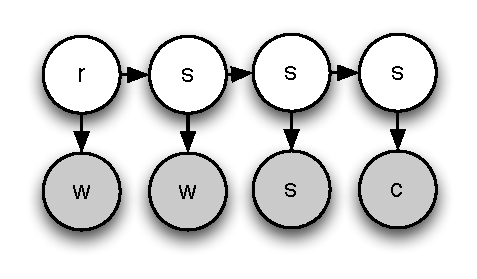
\includegraphics[scale=1]{figs/sequences/hmm}
\caption[HMM running example]{\label{fig:hmm} HMM structure, for the simple
running example.}
\end{figure}


A first order HMM model has the following independence assumptions over the joint distribution $\joint$:
\begin{itemize}
  \item \textbf{Independence of previous states.} The probability of
    being in a given state $\hv_l$ at position $\hs_i$ only depends on
    the state $\hv_m$ of the previous position $\hs_{i-1}$, that is 
    $p_{\theta} (\hs_i = \hv_l \mid \hs_{i-1} = \hv_m, \hs_{i-2} \ldots \hs_{1}) = p_{\theta} (\hs_i = \hv_l \mid \hs_{i-1} = \hv_m)$, 
    defining a first order Markov chain.%
    \footnote{The order of the Markov chain depends on the number of previous positions taken into account. 
    The remainder of the exposition can be easily extend to higher order HMM, giving the model more expressiveness, 
    but making inference harder.}
  \item \textbf{Homogeneous transition.} The probability of
    making a transition from state $\hv_l$ to state $\hv_m$ is independent of
    the particular position in the sentence, for all $i,j \in \{1,\ldots,N\}$:
    $p_{\theta} (\hs_i = \hv_l \mid \hs_{i-1} = \hv_m) =  p_{\theta}
    (\hs_j = \hv_l \mid \hs_{j-1} = \hv_m)$, so
    $p_{\theta} (\hs_i = \hv_l \mid \hs_{i-1} = \hv_m) = p_{\theta} (\hv_l \mid \hv_m)$.
  \item \textbf{Observation independence.}  The probability of
    observing $\vv_q$ at position $i$ is fully determined by the state
    at that position, that is  $p_{\theta}(\obs_i = \vv_q\mid
    \hs_i=\hv_l)$, and this probability is independent of the
    particular position, that is  $p_{\theta}(\obs_i = \vv_q\mid
    \hs_i=\hv_l)  = p_{\theta}(\vv_q\mid \hv_l)$.
\end{itemize}
These conditional independence assumptions are crucial to allow
efficient inference, as will be described. We also need to define a \emph{start probability}, the probability of starting 
at state $\hv_l$. Furthermore, when
dealing with text, it is usual to break the homogeneous transition
for the last position, and model the final transitions as 
independent parameters.
 The four probability
distributions that define the HMM model are summarized in Table
\ref{tab:hmm-dist}. 
For each one
of them we will use a short notation to simplify the exposition.
\begin{table}[h]
\begin{center}
\begin{tabular}{|l|l|l|}
\hline
\multicolumn{3}{|c|}{HMM distributions}\\
\hline
Name & probability distribution & short notation \\
\hline
\textbf{initial probability} & $p_{\theta} (\hs_1 = \hv_l)$ & $\pi_{l}$\\
\hline
\textbf{final probability} & $p_{\theta} (\hs_T = \hv_l \mid
\hs_{T-1} = \hv_m)$ & $f_{m,l}$\\
\hline
\textbf{transition probability} & $p_{\theta} (\hs_i = \hv_l \mid
\hs_{i-1} = \hv_m)$ & $a_{m,l}$\\
\hline
\textbf{observation probability} & $p_{\theta}(\obs_i = \vv_q\mid \hs_i = \hv_l)$ & $b_l(\obs_i) $ \\
\hline
\end{tabular}
\end{center}
\caption[HMM probability distributions]{\label{tab:hmm-dist} HMM probability distributions.}
\end{table}

The joint distribution can be expressed as:
\begin{equation}
  \joint =\pi_{\hs_1}b_{\hs_1}(\obs_1) [\prod_{i=2}^{N-1}
  a_{\hs_{i-1},\hs_{i}} b_{\hs_{i}}(\obs_i)] f_{\hs_{N-1},\hs_N}b_{\hs_{N}}(\obs_N),
  \label{eqn:hmm}
\end{equation}
which for the example from Figure \ref{fig:hmm} is:
\begin{equation}
  \joint =\pi_{r} b_r("w") a_{r,s}b_s("w") a_{s,s}b_s("s") f_{s,s}b_s("c").
  \label{eqn:hmm_ex}
\end{equation}

In the next section we turn our attention to estimating the different
probabilities distributions of the model  $\pi_l$, $a_{m,l}$,
$f_{m,l}$ and $b_l(\obs_i)$.

\begin{exercise}
Load the simple sequence dataset:
From the ipython command line (Note start ipython from the \emph{code}
directory), create a simple sequence object and look at the training
and test set.
\begin{python}
 In[]: run readers/simple_sequence.py
 In[]: simple = SimpleSequence()
 In[]: simple.train
Out[]: [w/r w/s s/s c/s , w/r w/r s/r c/s , w/s s/s s/s c/s ]
 In[]: simple.test
Out[]: [w/r w/s s/s c/s , c/s w/s t/s w/s ] 
\end{python}
\end{exercise}
%%% Local Variables: 
%%% mode: latex
%%% TeX-master: "../../guide"
%%% End: 






\section{\label{ml} Finding the Maximum Likelihood Parameters}
%So far we have not committed to any form for the probability
%distributions $\pi_l$, $a_{m,l}$ and $b_l(\obs_i)$. In both applications
%addressed in this class, both the observations and the hidden
%variables are discrete. The most common approach is to model each of
%these probability distributions as multinomial distributions,
%summarized in Table \ref{tt:mult-params}. Note that the number of parameters of $a_{l,m}$ is $|\hvocab|(|\hvocab|+1)$ because of the special ``STOP'' symbol.

%\begin{table}
%\begin{center}
%\begin{tabular}{|c|c|c|c|}
%\hline
%short notation & probability distribution  & |parameters|& constraint \\
%\hline
%$\pi_j$ & $p_{\theta} (\hs_1 = \hv_j)$ & $|\hvocab|$ & $\sum_{\hv \in \hvocab} \pi_j = 1$;\\
%\hline
%$a_{l,m}$ & $p_{\theta} (\hs_i = \hv_l \mid \hs_{i-1} = \hv_m)$ & $|\hvocab|(|\hvocab|+1)$ &$\sum_{\hv_l \in \hvocab} a_{m,l} = 1$;\\
%\hline
%%$f_{l,m}$ & $p_{\theta} (\hs_N = \hv_l \mid \hs_{N-1} = \hv_m)$ & $(|\hvocab|-1)^2$ &$\sum_{\hv_l \in \hvocab} t_{m,l} = 1$;\\
%%\hline
%$b_q(l) $& $p_{\theta}(\obs_i = \vv_q\mid \hs_i = \hv_l)$  & $|\hvocab||\vocab|$ &$\sum_{\vv_q \in \vocab} b_q(l)  = 1$.\\
%\hline
%\end{tabular}
%\end{center}
%\caption[HMM multinomial parametrization]{\label{tt:mult-params}Multinomial parametrization of the HMM distributions.}
%\end{table}

One important problem in HMMs is to estimate the 
model parameters, \emph{i.e.}, 
the distributions depicted in Table~\ref{tab:hmm-dist}. 
We will refer to the set of all these parameters 
as $\theta$. 
In a supervised setting, the HMM model
is trained to maximize the joint log-likelihood of the data. Given a
dataset $\mathcal{D}_L$, the objective being optimized is:
\begin{equation}
\argmax_{\theta} \sum_{m=1}^M \log P_{\theta}(X=x^m,Y=y^m),
\end{equation}
where $P_{\theta}(X=x^m,Y=y^m)$ is given by Eq.~\ref{eqn:hmm}.

In some applications (\emph{e.g.} speech recognition) 
the observation variables are continuous, hence the emission distributions are real-valued (\emph{e.g.} mixtures of Gaussians).
In our case, both the state set and the observation set are discrete (and finite), therefore we use
multinomial distributions for the emission and 
transition probabilities. 
Multinomial distributions are attractive for several reasons: first of
all, they are easy to implement; secondly, the maximum likelihood estimation of the parameters has a simple closed form. The parameters are just
normalized counts of events that occur in the corpus (the same as the
Na\"{i}ve Bayes from previous class).

Given our labeled corpus $\mathcal{D}_L$, the estimation process consists of counting how
many times each event occurs in the corpus and normalize the counts to
form proper probability distributions. Let us define the following
quantities, called sufficient statistics, that represent the counts of
each event in the corpus:

\begin{align}
\mathbf{Initial \ Counts\!:}\;\;\;\;  &  C_{\mathrm{init}}(c_k) = \sum_{m=1}^M
\Ind (y^m_1 = c_k); \label{eq::initialCounts}\\
%
%\mathbf{Final \ Counts\!:}\;\;\;\;  &  fc(\hv_l,\hv _m) = \sum_{\trex} 
%\Ind (\hs_N = \hv_l \mid \hs_{N-1} = \hv_m); \label{eq::finalCounts}\\
%
\mathbf{Transition \ Counts\!:}\;\;\;\;  &  C_{\mathrm{trans}}(c_k,c_l) =
\sum_{m=1}^M  \sum_{i = 2}^{N}
\Ind (y^m_i = c_k \wedge y^m_{i-1} = c_l); \label{eq::transitionCounts}\\
%
\mathbf{Final \ Counts\!:}\;\;\;\;  &  C_{\mathrm{final}}(c_k) = \sum_{m=1}^M
\Ind (y^m_N = c_k); \label{eq::finalCounts}\\
%
\mathbf{Emission \ Counts\!:}\;\;\;\;  &  
C_{\mathrm{emiss}}(w_j,c_k) = \sum_{m=1}^M
\sum_{i = 1}^{N}
\Ind (x^m_i = w_j \wedge y^m_i = c_k); \label{eq::emissionCounts}
\end{align}
Here $y^m_i$,  the underscript denotes the state index position for a given sequence, and the superscript denotes the sequence index in the dataset, and the same applies for the observations.
Note that $\Ind$ is an indicator function that has the value 1 when the
particular event happens, and zero otherwise. In other words, the previous
equations go through the training corpus and count how
often each event occurs. For example, Eq.~\ref{eq::transitionCounts} counts how many times $c_k$ follows state $c_l$. Therefore, $C_{\mathrm{trans}}(\text{\tt sunny},\text{\tt rainy})$ contains the number of times that a sunny day followed a rainy day.

%
%: e.g. the word ``w'' appears with state
%``s'', or state ``s'' follows another state ``s'', or state ``s''
%begins the sentence.


After computing the counts, one can perform some sanity checks
to make sure the implementation is correct. Summing over all entries
of each count table we should observe the following:

\begin{itemize}
\item \textbf{Initial \ Counts\!:} -- Should sum to the number of
  sentences: $\sum_{k=1}^K C_{\mathrm{init}}(c_k) = M$
%\item \textbf{Final \ Counts\!:} - Should sum to the number of sentences.
\item \textbf{Transition/Final \ Counts\!:} -- Should sum to the number of
  tokens: 
  $\sum_{k,l=1}^K C_{\mathrm{trans}}(c_k,c_l) + \sum_{k=1}^K C_{\mathrm{final}}(c_k) = MN$
%   minus 2 times the number of sentences. Note that there are
%  N-1 edges for each sentence, and the last edge is being accounted by
%  the final transitions. So this leaves us with N-2 edges per sentence,
%  where N is the number of tokens in that sentence.
\item \textbf{Observation \ Counts\!:} -- Should sum to the number of tokens: $\sum_{j=1}^J\sum_{k=1}^K C_{\mathrm{emiss}}(w_j,c_k) = MN$.
\end{itemize}

Using the sufficient statistics (counts) the parameter estimates are: 
\begin{align}
  P_{\mathrm{init}}(c_k | \text{\tt start}) &=  \frac{C_{\mathrm{init}}(c_k)}{\sum_{l=1}^K
    C_{\mathrm{init}}(c_l)}\\
  P_{\mathrm{final}}(\text{\tt stop} | c_l) &=  \frac{C_{\mathrm{final}}(c_l)}{\sum_{k=1}^K
    C_{\mathrm{trans}}(c_k,c_l) + C_{\mathrm{final}}(c_l)}\\
  P_{\mathrm{trans}}(c_k | c_l) &=  \frac{C_{\mathrm{trans}}(c_k,c_l)}{\sum_{p=1}^K
    C_{\mathrm{trans}}(c_p,c_l) + C_{\mathrm{final}}(c_l)}\\
  P_{\mathrm{emiss}}(w_j | c_k) &=  \frac{C_{\mathrm{emiss}}(w_j,c_k)}{\sum_{q=1}^J
    C_{\mathrm{emiss}}(w_q,c_k)}
\end{align}


%\begin{exercise}
%Convince yourself that the sanity checks described above are true.
%Collect the counts from a supervised corpus using method
%\emph{collect\_counts\_from\_corpus} and use the provided function \emph{sanity\_check\_counts} to perform these checks on the counts table. 
%%\begin{python}
%% def sanity_check_counts(self,seq_list):
%%\end{python}
%
%\begin{python}
%>>> import sequences.hmm as hmmc
%>>> hmm = hmmc.HMM(simple.x_dict, simple.y_dict)
%>>> hmm.train_supervised(simple.train)
%>>> hmm.sanity_check_counts(simple.train)
%>>> print "Initial Probabilities:", hmm.initial_probs
%
%>>> print "Transition Probabilities:", hmm.transition_probs
%
%>>> print "Final Probabilities:", print 
%hmm.final_probs
%
%>>> print "Emission Probabilities", print hmm.emission_probs
%
%Initial counts match
%Final counts match
%Transition counts match
%Observations counts match
%\end{python}
%\end{exercise}



\begin{exercise}
The provided function \emph{train\_supervised} from the \emph{hmm.py} file implements the above parameter estimates.
%Implement a function that estimates the maximum likelihood
%estimates for the parameters given the corpus in the class HMM.
%The function header is in the hmm.py file. 
%\begin{python}
%def train_supervised(self,sequence_list):
%\end{python}
Run this function given the simple dataset above and look at the estimated probabilities. Are they correct? You can also check the variables ending in \emph{\_counts} instead of \emph{\_probs} to see the raw counts (for example, typing \emph{hmm.initial\_counts} will show you the raw counts of initial states). How are the counts related to the probabilities?

\begin{python}
>>> import lxmls.sequences.hmm as hmmc
>>> hmm = hmmc.HMM(simple.x_dict, simple.y_dict)
>>> hmm.train_supervised(simple.train)
>>> print "Initial Probabilities:", hmm.initial_probs
[ 0.66666667  0.33333333]
>>> print "Transition Probabilities:", hmm.transition_probs
[[ 0.5    0.   ]
 [ 0.5    0.625]]
>>> print "Final Probabilities:", hmm.final_probs
[ 0.     0.375]
>>> print "Emission Probabilities", hmm.emission_probs
[[ 0.75   0.25 ]
 [ 0.25   0.375]
 [ 0.     0.375]
 [ 0.     0.   ]]
\end{python}
\end{exercise}


%%% Local Variables: 
%%% mode: latex
%%% TeX-master: "../../guide"
%%% End: 




\section{\label{decoding} Decoding a Sequence}
Given the learned parameters and a new
observation sequence $x = x_1\ldots x_N$, we want to find the sequence of hidden states $y^* = y_1^* \ldots y_N^*$ that ``best'' explains it.
 This is called the \emph{decoding} problem. There are several ways to define what we mean by the ``best''
$y^*$, depending on our goal: for instance, we may want to minimize the probability of error
on each hidden
variable $Y_i$, or we may want to find the best assignment
to the sequence $Y_1\ldots Y_N$ as a whole. 
Therefore, finding the best sequence
can be accomplished through different approaches:

\begin{itemize}
\item A first approach, normally called \textbf{posterior decoding} or \textbf{minimum risk decoding}, consists
in picking the highest state posterior for each position $i$ in the sequence:
\begin{equation}
y_i^* = \argmax_{y_i \in \Lambda} P(Y_i=y_i | X_1=x_1,\ldots,X_N =x_N).
\end{equation}
%where $\gamma_i(\hs_i)$ is the posterior probability $P(\hs_i|\sent)$. 
Note, however, that this approach does not guarantee that the sequence $y^*=y_1^* \ldots y_N^*$ will be a
valid sequence of the model. For instance, there might be a transition
between two of the best state posteriors with probability zero. 

\item A second approach, called \textbf{Viterbi decoding}, consists in
picking the best global hidden state sequence: 
\begin{eqnarray}
y^* &=& \argmax_{y = y_1\ldots y_N} P(Y_1=y_1,\ldots, Y_N=y_N | X_1=x_1,\ldots,X_N =x_N)\nonumber\\
&=& \argmax_{y = y_1\ldots y_N} P(Y_1=y_1,\ldots, Y_N=y_N, X_1=x_1,\ldots,X_N =x_N).
\end{eqnarray}
\end{itemize}

Both approaches (which will be explained in Sections~\ref{posterior} and~\ref{viterbi}, respectively) rely on dynamic programming and make use of the
independence assumptions of the HMM model. Moreover, they use an alternative
representation of the HMM called a \emph{trellis}. 

A trellis unfolds all possible states for each position and it makes explicit the independence assumption: each position only
depends on the previous position. Here, each column represents a position in the sequence and each row represents a possible state. Figure \ref{fig:trellis} shows the
trellis for the particular example in Figure \ref{fig:hmm}. 

\begin{figure}[ht]
\centering
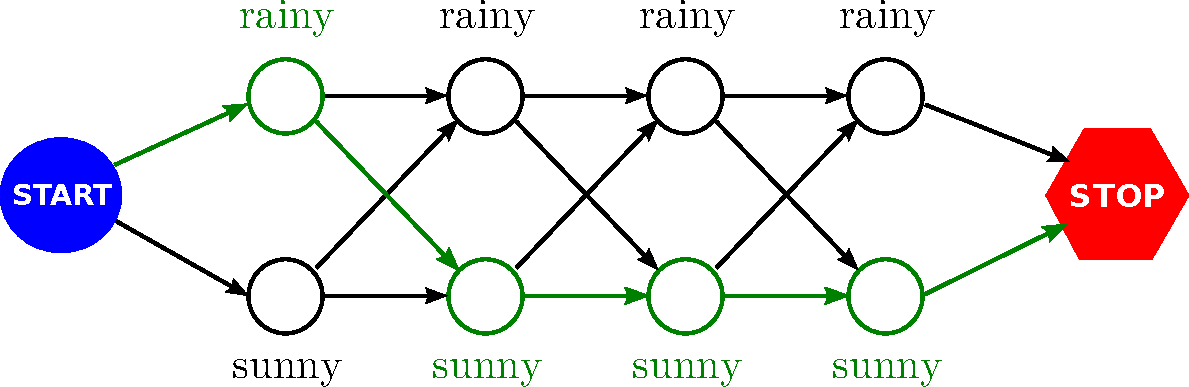
\includegraphics[width=0.7\textwidth]{figs/sequences/trellis_new}
\caption[HMM Trellis representation.]{\label{fig:trellis} Trellis
  representation of the HMM in Figure ~\ref{fig:hmm}, for the observation
  sequence ``{\tt walk} {\tt walk} {\tt shop} {\tt clean}'', where each hidden variable can take the values {\tt rainy} or {\tt sunny}.}
\end{figure}




Considering the trellis representation, note that we can include the following information:
\begin{itemize}
\item an \emph{initial probability} to the arrows that depart from the start symbol;
\item a \emph{final probability} to the arrows that reach the stop symbol;
\item a \emph{transition probability} to the remaining arrows; and,
\item an \emph{emission probability} to each circle, which is the probability that the observed symbol is emitted by that particular state.
\end{itemize}

For convenience, we will be working with 
log-probabilities, rather than probabilities.\footnote{This will be motivated further in Section~\ref{sec:logdomain}, where we describe 
how operations can be performed efficiently
in the log-domain.} Therefore, if we associate to each circle and arrow in
the trellis a score that corresponds
to the log-probabilities above, 
and if we define the score of a path
connecting the {\tt start} and  {\tt stop} symbols as
the sum of the scores of the circles and arrows
it traverses, 
then 
the goal of finding the most likely sequence of states (Viterbi decoding) corresponds to 
finding the path with the highest score.




%---since 
%we'll be multiplying a lot of probabilities, 
%we prevent underflowing by working in the log-domain. 

%For the decoding algorithms described in the following sections, 
%it is
%useful to define a re-parametrization of the model in equation \eqref{eqn:hmm}, in terms of
%node potentials $\phi_n(l)$ (associating a number to each box in Figure \ref{fig:trellis})
%and edge potentials $\phi_{n-1,n}(l,m)$ (associating a number to each edge in  Figure
%\ref{fig:trellis}). For our example, this re-parametrization is given by
%%
%\begin{equation}
%  \joint =\phi_1(r)\phi_1(r,s)\phi_2(s)\phi_2(s,s)\phi_3(s)\phi_3(s,s)\phi_4(s).
%  \label{eqn:hmm_ex_treelis}
%\end{equation}
%
%%\begin{equation}
%%  \joint =\phi_1(``w'',r)\phi_1(r,s)\phi_2(``w'',s)\phi_2(s,s)\phi_3(``s'',s)\phi_3(s,s)\phi_4(``c'',s).
%%  \label{eqn:hmm_ex_treelis}
%%\end{equation}
%
%In other words, to do this re-parameterization we need to find expressions for the potential variables, (the $\phi$'s) such that \eqref{eqn:hmm} and \eqref{eqn:hmm_ex_treelis} are equal. The solution is given by
%\begin{equation}
%\phi_{i-1,i}(l,m) = a_{l,m}
%\label{eq:nodes1}
%\end{equation}
%and
%\begin{equation}
%\phi_i(l) = 
%\begin{cases}
% b_{\obs_i}(l)\pi_l \quad\text{i = 1}\\
% b_{\obs_i}(l) \quad\text{i = 2,\ldots,N-1}\\
% b_{\obs_i}(l)a_{l,STOP} \quad\text{i = N}
% \label{eq:nodes2}
%\end{cases}
%\end{equation}


%\begin{itemize}
%\item\emph{Edge Potentials} - correspond to the transition parameters, with the exception of the
%edges into the last position that correspond to the final transition parameters.
%\item\emph{Node Potentials} - correspond to the observation
%parameters for a given state and the observation at that position.  The
%first position is the exception and corresponds to the
%product between the observation parameters for that state and
%the observation in that position with the initial parameters for that state. 
%\end{itemize}

%Although this re-parametrization simplifies the exposition, and will be
%used in these lectures, it is not necessarily very practical since we
%will be reproducing several values (for instance the transition
%parameters for each position).


The trellis scores are given by the following expressions:
\begin{itemize}
\item For each state $c_k$:
\begin{eqnarray}
\mathrm{score}_{\mathrm{init}}(c_k) &=&
\log P_{\mathrm{init}}(Y_{1} = c_k | \text{\tt start}).
\end{eqnarray}
\item For each position $i \in {1,\ldots,N-1}$ and each pair of states $c_k$ and $c_l$:
\begin{eqnarray}
\mathrm{score}_{\mathrm{trans}}(i, c_k, c_l) &=&
\log P_{\mathrm{trans}}(Y_{i+1} = c_k | Y_i = c_l).
\end{eqnarray}
\item For each state $c_l$:
\begin{eqnarray}
\mathrm{score}_{\mathrm{final}}(c_l) &=&
\log P_{\mathrm{final}}(\text{\tt stop} | Y_N = c_l).
\end{eqnarray}
\item For each position $i \in {1,\ldots,N}$ and state $c_k$:
\begin{eqnarray}
\mathrm{score}_{\mathrm{emiss}}(i, c_k) &=&
\log P_{\mathrm{emiss}}(X_i = x_i | Y_i = c_k).
\end{eqnarray}
\end{itemize}

In the next exercise, you will compute the trellis scores.

\begin{exercise}
Convince yourself that the score of a path in the trellis 
(summing over the scores above) is equivalent 
to the log-probability $\log P(X=x,Y=y)$, 
as defined in 
Eq.~\ref{eqn:hmm_ex}. 
Use the given function \emph{compute\_scores} on the first training sequence and confirm that the values are correct. You should get the same values as presented below.

%Implement a function that builds the node and edge potentials for a
%given sequence. The function head is in the \emph{hmm.py} file:

%\begin{python}
% def build_potentials(self,sequence):
%\end{python}
%
%Run this function for the first training sequence from the simple
%dataset and compare the results given (If the results are the same
%then you are ready to go).

\begin{python}
initial_scores, transition_scores, final_scores, emission_scores = hmm.compute_scores(simple.train.seq_list[0])
print initial_scores

[-0.40546511 -1.09861229]

print transition_scores

[[[-0.69314718        -inf]
  [-0.69314718 -0.47000363]]

 [[-0.69314718        -inf]
  [-0.69314718 -0.47000363]]

 [[-0.69314718        -inf]
  [-0.69314718 -0.47000363]]]

print final_scores

[       -inf -0.98082925]

print emission_scores

[[-0.28768207 -1.38629436]
 [-0.28768207 -1.38629436]
 [-1.38629436 -0.98082925]
 [       -inf -0.98082925]] 
\end{python}

Note that scores which are $-\infty$ (\texttt{-inf}) correspond
to zero-probability events. 
\end{exercise}

\subsection{Computing in log-domain}\label{sec:logdomain}

We will see that the decoding algorithms 
will need to multiply twice as many probability terms as 
the length $N$ of the sequence. 
This may cause underflowing problems 
when $N$ is large, since the nested multiplication of numbers smaller than 1
may easily become smaller than the machine precision. To avoid that
problem, \cite{rabiner} presents a scaled version of the decoding algorithms that avoids this problem.
An alternative, which is widely used, is computing
in the log-domain. That is, instead of 
manipulating probabilities, manipulate log-probabilities (the scores presented above). 
Every time we need to multiply probabilities, 
we can sum their log-representations, since:
\begin{equation}
\log(\exp(a) \times \exp(b)) = a+b.
\end{equation}
Sometimes, we need to \emph{add} probabilities. 
In the log domain, this requires us to compute 
\begin{equation}
\log(\exp(a) + \exp(b)) = a + \log(1 + \exp(b-a)),
\end{equation}
where we assume that $a$ is smaller than $b$.


\begin{exercise}
Look at the module {\tt sequences/log\_domain.py}. 
This module implements a function
{\tt logsum\_pair(logx, logy)} to 
add two numbers represented in the log-domain;
it returns their sum also represented in the log-domain. The function {\tt logsum(logv)} 
sums all components of an array 
represented in the log-domain. 
This will be used later in our decoding algorithms.
To observe why this is important, type the 
following:
\begin{python}
import numpy as np
a = np.random.rand(10)
np.log(sum(np.exp(a)))
2.8397172643228661

np.log(sum(np.exp(10*a)))
10.121099917705818

np.log(sum(np.exp(100*a)))
93.159220940569128

np.log(sum(np.exp(1000*a)))
inf

from lxmls.sequences.log_domain import *
logsum(a)
2.8397172643228665

logsum(10*a)
10.121099917705818

logsum(100*a)
93.159220940569114

logsum(1000*a)
925.88496219586864
\end{python}
\end{exercise}


\subsection{Posterior Decoding}\label{posterior}
Posterior decoding consists
in picking state with the highest posterior for each position in the sequence independently; for 
each $i = 1,\ldots,N$:
\begin{equation}
y_i^* = \argmax_{y_i \in \statevocab} P(Y_i=y_i | X = x).
\end{equation}
The \textbf{sequence posterior distribution} is the probability of a particular
hidden state sequence given that we have observed a particular
sequence. Moreover, we will be interested in two other posteriors distributions:
the \textbf{state posterior distribution}, corresponding to the
probability of being in a given state in a certain position given the
observed sequence; and the \textbf{transition posterior distribution},
which is the probability of making a particular transition, from position $i$ to
$i+1$, given the observed sequence. They are formally defined as follows:
\begin{align}
  \mathbf{Sequence \ Posterior\!:}\;\;\;\; &P(Y=y|X=x) = \frac{P(X=x,Y=y)}{P(X=x)}; \label{eq::posteriorDistribution} \\
 \mathbf{State \ Posterior\!:}\;\;\;\;  & P(Y_i=y_i | X=x); \label{eq::nodePosterior} \\
 \mathbf{Transition \ Posterior\!:}\;\;\;\;  &P(Y_{i+1}=y_{i+1},Y_i=y_i| X=x).\label{eq::edgePosterior}
\end{align}

To compute the posteriors, a first step is to be able to compute the 
likelihood of
the sequence $P(X=x)$, which corresponds to summing the probability of all
possible hidden state sequences.
\begin{equation}
\label{likelihoood}
\mathbf{Likelihood\!:}\;\;\;\; P(X=x) = \displaystyle \sum_{y \in \statevocab^N} P(X=x,Y=y).
\end{equation}
The number of possible hidden state sequences is exponential in the
length of the sequence ($|\statevocab|^N$),
 which makes the sum over all of them hard. 
 In our simple
 example, there are $2^4 = 16$ paths, which we can actually explicitly enumerate
 and calculate their probability using Equation \ref{eqn:hmm}. But this is as far as it goes: for example, for Part-of-Speech
 tagging with a small tagset of 12 tags and a medium size
 sentence of length 10, there are $12^{10} = 61 917 364 224$ such
 paths. 
Yet, we must be able to compute this sum (sum over $y \in \statevocab^N$) to compute the above likelihood
formula; this is called the inference problem. For sequence models, there is a well known dynamic programming algorithm,
the \textbf{Forward-Backward} (FB) algorithm, which allows the computation
to be performed in linear time,%
\footnote{The runtime is linear with respect
to the sequence length. More precisely, 
the runtime is $O(N|\statevocab|^2)$. 
A naive enumeration would cost $O(|\statevocab|^N)$.} %
by making use of the independence assumptions.

The FB algorithm relies on the independence of previous states
assumption, which  
is illustrated in the trellis view by having arrows only between consecutive states. 
The FB algorithm defines two auxiliary probabilities, the forward probability and the backward probability. 

\subsection*{Efficient forward probability computation}
The forward probability represents the probability that in position
$i$ we are in state $Y_i = c_k$ and that we have observed $x_1,\ldots,x_i$
up to that position. Therefore, its mathematical expression is:
\begin{equation}
\label{eq::forward}
\mathbf{Forward \ Probability\!:}\;\;\;\;  \mathrm{forward}(i, c_k) = P(Y_i = c_k, X_1=x_1,\ldots, X_i = x_i)
\end{equation}

Using the independence assumptions of the HMM we can compute $\mathrm{forward}(i, c_k)$ using all the forward computations \{$\mathrm{forward}(i -1, c)$ for $c \in \statevocab$\}. In order to facilitate the notation of the following argument we will denote by $x_{i:j}$  the assignemnt $X_i = x_i, \dots, X_j = x_j$. Therefore we can write   $\mathrm{forward}(i, y_i) $ as $P( y_i, x_{1:i } ) $ and rewrite the forward expression as follows:
\begin{equation}
\label{eq::forward2}
  P( y_i, x_{1:i } ) =  \sum_{y_{i-1} \in \statevocab} P( y_i ,y_{i-1}, x_{1:i } )  =  \sum_{y_{i-1} \in \statevocab} P( x_i  | y_i,  y_{i-1},  x_{1:i-1 } ) \cdot P(y_i  | y_{i-1},  x_{1:i-1 }) \cdot P(y_{i-1},  x_{1:i-1 })  
\end{equation}

Using the \textbf{Observation independence} and the \textbf{Independence of previous states} properties of the first order HMM we have $P( x_i  | y_i,  y_{i-1},  x_{1:i-1 } ) = P( x_i  | y_i) $ and $P(y_i  | y_{i-1},  x_{1:i-1 })  = P(y_i  | y_{i-1})  $. Therefore equation (\ref{eq::forward2}) can be written, 
for $i \in \{2,\dots,N\}$ (where $N$ is the length of the sequence), as 
\begin{equation}
\label{eq::forward3}
 \mathrm{forward}(i, y_i)  = \sum_{y_{i-1} \in \statevocab} P( x_i  | y_i, ) \cdot P(y_i  | y_{i-1}) \cdot \mathrm{forward}(i-1, y_{i-1})   
\end{equation}

 Using equation (\ref{eq::forward3}) we have proved that  the forward probability can be defined by the
following recurrence rule: 
\begin{eqnarray}
\mathrm{forward}(1, c_k)&=& P_{\mathrm{init}}(c_k|\text{\tt start}) \times 
P_{\mathrm{emiss}}(x_1 | c_k)
 \\
 \mathrm{forward}(i, c_k) &=& \left( \displaystyle \sum_{c_l \in \statevocab} P_{\mathrm{trans}}(c_k | c_l) \times \mathrm{forward}(i-1, c_l) \right) \times P_{\mathrm{emiss}}(x_i | c_k)  \label{forwardRecursion}
 \\
  \mathrm{forward}(N+1, \text{\tt stop}) &=& \sum_{c_l \in \statevocab} P_{\mathrm{final}}(\text{\tt stop} | c_l) \times \mathrm{forward}(N, c_l).
\end{eqnarray}

%\begin{figure}
%\begin{center}
%\begin{tabular}{cc}
%
%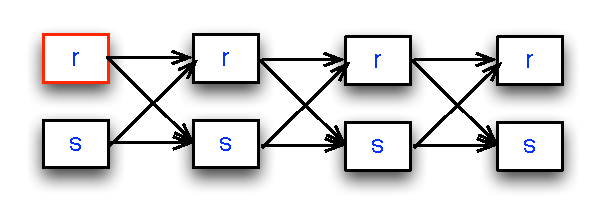
\includegraphics[scale=.5]{figs/sequences/forward1}
%& 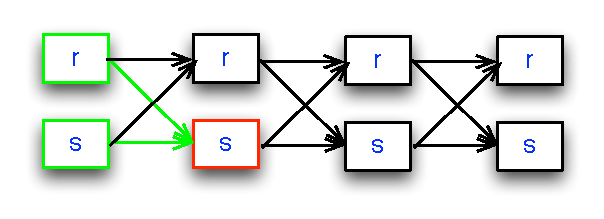
\includegraphics[scale=.5]{figs/sequences/forward2}\\
%\end{tabular}
%\caption[Forward-backward example.]{\label{fig:fb} Forward trellis for
%  the first sentence of the training data at position 1 (left) and at
%  position 2 (right)}
%
%\end{center}
%\end{figure}

%At position 1, the probability of being in state ``r'' and observing word ``w'' is just the node
%marginal for that position: $\alpha_1(r) = \phi_1(r)$ (see Figure
% \ref{fig:fb} left). At position 2 the probability
%of being in state ``s'' and observing the sequence of words ``w w''
%corresponds to the sum of all possible ways of reaching position 2 in
%state ``s'', namely, ``rs'' and ``ss'' (see Figure \ref{fig:fb} right). The probability of the former is
%$\phi_1(r)\phi_1(r,s)\phi_2(s)$
%and that of the latter is $\phi_1(s)\phi_1(s,s)\phi_2(s)$, so we get:
%\begin{eqnarray*}
%   \alpha_2(s) &=& \phi_1(r)\phi_1(r,s)\phi_2(s) +
%   \phi_1(s)\phi_1(s,s)\phi_2(s) \\
%   \alpha_2(s) &=& \left[\phi_1(r)\phi_1(r,s) +
%   \phi_1(s)\phi_1(s,s) \right]\phi_2(s) \\
% \alpha_2(s) &=& \displaystyle \sum_{\hs \in \hvocab}
% \left[\phi_1(\hs)\phi_1(\hs,s)\phi_2(s) \right] \\
%  \alpha_2(s) &=& \displaystyle \sum_{\hs \in \hvocab}
% \left[\alpha_1(\hs)\phi_1(\hs,s)\phi_2(s) \right]
%\end{eqnarray*}

Using the forward trellis one can compute the likelihood simply as:
\begin{equation}
\label{eq:forwardSum}
P(X=x) = \mathrm{forward}(N+1, \text{\tt stop}).
\end{equation}

Although the forward probability is enough to calculate the likelihood of a given sequence, we will also need the backward probability to calculate the state posteriors. 

% We could include a graph and comment the d-separation property which implies the conditional independence assumptions of the HMM graphically.
%\begin{figure}[ht]
%\centering
%\includegraphics[width=0.5\textwidth]{figs/sequences/hmm_diagram}
%\caption[HMM diagram]{\label{fig:hmm_diagram}Diagram showing the conditional independence relations of the HMM. If $Y_i$ is observed then...}
%\end{figure}

\subsection*{Efficient backward probability computation}

The backward probability is similar to the forward probability, but operates in the inverse direction.
It represents the probability of observing $x_{i+1},\ldots,x_N$ from position $i+1$ up to $N$, given that at position $i$ we are at state $Y_i = c_l$:
 \begin{equation}
\label{eq::backward}
\mathbf{Backward \ Probability\!:}\;\;\;\;  \mathrm{backward}(i, c_l) = P(X_{i+1}=x_{i+1},\ldots, X_N=x_N | Y_i = c_l).
\end{equation}

Using the independence assumptions of the HMM we can compute $\mathrm{backward}(i, c_k)$ using all the backward computations \{$\mathrm{backward}(i +1, c)$ for $c \in \statevocab$\}. Therefore we can write   $\mathrm{backward}(i, y_i) $ as $P( x_{i+1:N} | y_i ) $ and rewrite the forward expression as follows:
\begin{equation}
\label{eq::backward2}
  P( x_{i+1:N} | y_i ) =  \sum_{y_{i+1} \in \statevocab} P( x_{i+1:N}, y_{i+1} | y_i)  =  \sum_{y_{i+1} \in \statevocab} P( x_{i+2:N} | y_i, y_{i+1}, x_{i+1}) 
   P( x_{i+1}, |  y_{i+1},  y_{i}) P( y_{i+1} | y_i)
\end{equation}

Using the previous equation we have proved that the backward probability can be defined by the following recurrence rule:

\begin{eqnarray}
\mathrm{backward}(N, c_l) &=& P_{\mathrm{final}}(\text{\tt stop} | c_l) 
 \\
 \mathrm{backward}(i, c_l) &=&  \displaystyle \sum_{c_k \in \statevocab} P_{\mathrm{trans}}(c_k | c_l) \times \mathrm{backward}(i+1, c_k) \times P_{\mathrm{emiss}}(x_{i+1} | c_k)  \label{backwardRecursion}
 \\
  \mathrm{backward}(0, \text{\tt start}) &=& \sum_{c_k \in \statevocab} P_{\mathrm{init}}(c_k | \text{\tt start}) \times \mathrm{backward}(1, c_k) \times P_{\mathrm{emiss}}(x_{1} | c_k).
\end{eqnarray}
%At position $N$ there are no more observations, and the backward
%probability is set to 1. At position $i$, the probability 
%of having observed the future and being in state $\hv_l$, is given by the sum for all possible states of the probability of having transitioned 
%from position $i$ with state $\hv_l$ to position $i+1$ with state $\hv_m$, and observing $\obs_{i+1}$ at time $i+1$ and the future from there onward, which is $\beta_{i+1}(\hs_{i+1} = \hv_m)$. 
Using the backward trellis one can compute the likelihood simply as:.
\begin{equation}
\label{eq:backwardSum}
P(X=x) = \mathrm{backward}(0, \text{\tt start}).
\end{equation}

\subsection*{The forward backward algorithm}

We have seen how we can compute the probability of a sequence $x$ using the the forward and backward probabilities by computing  $\mathrm{forward}(N+1, \text{\tt stop})$ and $ \mathrm{backward}(0, \text{\tt start})$ respectively. Moreover,  the probability of a sequence $x$ can be computed with both forward and backward probabilities at a particular position $i$. The probability of a  given sequence $x$ at any position $i$ in the sequence can be computed
as follows \footnote{ The second equality in \ref{eq::fbsanity} can be justified as follows. Since $Y_i=y_i$ is observed then  $X_{i+1}, \dots, X_{N}$ is conditionally independent from any $X_k$ for $k \leq i$ . Therefore  $P(x_1,\dots, x_N, y_i) =  P( x_{i+1},\dots, x_N �| yi , x_1, \dots,x_i ) \cdot P( yi , x_1, \dots,x_i ) =  P( x_{i+1},\dots, x_N �| yi  ) \cdot P( yi , x_1, \dots,x_i ) = backward(i,y_i) \cdot forward(i,y_i)$.}:


\begin{eqnarray}
\label{eq::fbsanity}
  P(X=x) &=& 
  \sum_{c_k \in \statevocab} P(X_1=x_1,\ldots, X_N=x_N,Y_i=c_k)\nonumber\\
  & =&
  \sum_{c_k \in \statevocab} 
  \underbrace{P(X_1=x_1,\ldots, X_i=x_i, Y_i=c_k)}_{\mathrm{forward}(i,c_k)} \times 
  \underbrace{P(X_{i+1}=x_{i+1},\ldots, X_N=x_N| Y_i=c_k)}_{\mathrm{backward}(i,c_k)}\nonumber\\
  &=& \sum_{c_k \in \statevocab} \mathrm{forward}(i,c_k) \times \mathrm{backward}(i,c_k).
\end{eqnarray}


This equation will work for any choice of $i$. Although redundant, this fact is useful when implementing an
HMM as a sanity check that the computations are being performed
correctly, since one can compute this expression for several $i$; they should all yield the same value. 

Algorithm \ref{alg:fb} shows the pseudo code for the forward backward algorithm. The reader can notice that the $forward$ and $backward$ computations in the algorithm make use of $P_{emiss}$ and $P_{trans}$. There are a couple of details that should be taken into account if the reader wants to understand the algorithm using scores instead of probabilities.

% maybe more details on how to implement the algorithm using "scores" instead of probabilities should be given. 
\begin{itemize}
\item  $forward(i,\hat{c})$  is computed using $P_{emiss}(x_i | \hat{c})$ which does not depend on the sum over all possible states $c_k \in  \statevocab $. Therefore when taking the logarithm of the sum over all possible states the recurrence of the forward computations can be split as a sum of two logarithms.
\item $backward(i,\hat{c})$  is computed using $ P_{\mathrm{trans}}(c_k | \hat{c} )$ and $P_{\mathrm{emiss}}(x_{i+1} | c_k) $ both of  which  depend on $c_k$. Therefore when taking the logarithm of the sum the expression cannot be split as a sum of logarithms.
\end{itemize}


\begin{algorithm}[t]
   \caption{Forward-Backward algorithm \label{alg:fb}}
\begin{algorithmic}[1]
   \STATE {\bfseries input:} sequence $x_1,\ldots,x_N$, scores $P_{\mathrm{init}}, P_{\mathrm{trans}}, P_{\mathrm{final}}, P_{\mathrm{emiss}}$
        \item[]
        \STATE  \emph{Forward pass}: Compute the forward probabilities
        %\STATE \emph{Initialization}
        \FOR{$c_k \in \statevocab$ }
        \STATE $\mathrm{forward}(1,c_k) = P_{\mathrm{init}}(c_k|\text{\tt start}) \times 
P_{\mathrm{emiss}}(x_1 | c_k)$
        \ENDFOR 
        \FOR{$i=2$ {\bfseries to} $N$}
         \FOR{$\hat{c} \in \statevocab$ }
                 \STATE $\mathrm{forward}(i, \hat{c} ) = \left( \displaystyle \sum_{c_k \in \statevocab} P_{\mathrm{trans}}(\hat{c}| c_k) \times \mathrm{forward}(i-1, c_k) \right) \times P_{\mathrm{emiss}}(x_i | \hat{c})$
         \ENDFOR 
        \ENDFOR 
       \item[]
       \STATE \emph{Backward pass}: Compute the backward probabilities
      % \STATE \emph{Initialization}
        \FOR{$c_k \in \statevocab$ }
        \STATE $\mathrm{backward}(N, c_k) = P_{\mathrm{final}}(\text{\tt stop} | c_k)$
        \ENDFOR 
       \FOR{$i=N-1$ {\bfseries to} 1}
                 \FOR{$\hat{c} \in \statevocab$ }
       \STATE $\mathrm{backward}(i, \hat{c}) =  \displaystyle \sum_{c_k \in \statevocab} P_{\mathrm{trans}}(c_k | \hat{c} ) \times \mathrm{backward}(i+1, c_k) \times P_{\mathrm{emiss}}(x_{i+1} | c_k)$
       	 \ENDFOR 
        \ENDFOR 
        \item[]
       \STATE \textbf{output:} The forward and backward probabilities.
\end{algorithmic}
\end{algorithm}




\begin{exercise}
%Given the implementation of the forward pass of the forward backward
%algorithm in the file \emph{forward\_backward.py}, implement the backward pass.
%\begin{python}
%
%def forward_backward(node_potentials,edge_potentials):
%    H,N = node_potentials.shape
%    forward = np.zeros([H,N],dtype=float)
%    backward = np.zeros([H,N],dtype=float)
%    forward[:,0] = node_potentials[:,0]
%    ## Forward loop
%    for pos in xrange(1,N):
%        for current_state in xrange(H):
%            for prev_state in xrange(H):
%                forward_v = forward[prev_state,pos-1]
%                trans_v = edge_potentials[prev_state,current_state,pos-1]
%                prob = forward_v*trans_v
%                forward[current_state,pos] += prob
%            forward[current_state,pos] *= node_potentials[current_state,pos]
%    ## Backward loop
%          ## Your code
%   return forward,backward
%
%\end{python}

Run the provided forward-backward algorithm on the first train sequence. 
Observe that both the forward and the backward 
passes give the same log-likelihood.
%Use the provided function that makes use of Equation \ref{eq::fbsanity} to make
%sure your implementation is correct: 
\begin{python}
log_likelihood, forward = hmm.decoder.run_forward(initial_scores, transition_scores, final_scores, emission_scores)
print 'Log-Likelihood =', log_likelihood

Log-Likelihood = -5.06823232601

log_likelihood, backward = hmm.decoder.run_backward(initial_scores, transition_scores, final_scores, emission_scores)
print 'Log-Likelihood =', log_likelihood

Log-Likelihood = -5.06823232601
\end{python}
\end{exercise}


Given the forward and backward probabilities, one can compute both the state
and transition posteriors 
(you can hint why by looking at the term inside the sum in Eq.~\ref{eq::fbsanity}).


\begin{align}
 \mathbf{State \ Posterior\!:}\;\;\;\;  & P(Y_i = y_i| X=x) = \frac{\mathrm{forward}(i, y_i) \times 
 \mathrm{backward}(i, y_i)}{P(X=x)}; \label{eq::nodePosterior2} \\
 \mathbf{Transition \ Posterior\!:}\;\;\;\; &
 P(Y_i = y_i, Y_{i+1} = y_{i+1} | X=x)= \nonumber\\
 &
   \frac{\mathrm{forward}(i, y_i) \times 
   P_{\mathrm{trans}}(y_{i+1}|y_i) \times
   P_{\mathrm{emiss}}(x_{i+1}|y_{i+1}) \times
 \mathrm{backward}(i+1, y_{i+1})}{P(X=x)}.\label{eq::edgePosterior2}
\end{align}

A graphical representation of these posteriors is illustrated in Figure~\ref{fig:posteriors}. 
On the left it is shown that $\mathrm{forward}(i, y_i)  \times \mathrm{backward}(i, y_i)$ returns the sum of all paths that contain the state $y_i$, weighted by $P(X=x)$; on the right we can see that $\mathrm{forward}(i, y_i) \times P_{\mathrm{trans}}(y_{i+1}|y_i) \times P_{\mathrm{emiss}}(x_{i+1}|y_{i+1}) \times \mathrm{backward}(i+1, y_{i+1})$  returns the same for all paths containing the edge from $y_i$ to $y_{i+1}$.
%Thus, these posteriors can be seen as the ratio of the number of paths that contain the given state or transition (weighted by $P(X=x)$) and the number of possible paths in the graph $\marginal$.

As a practical example, given that the person performs the sequence of actions ``{\tt walk} {\tt walk} {\tt shop} {\tt clean}", we want to know the probability of having been raining in the second day. The state posterior probability for this event can be seen as the probability that the sequence of actions above was generated by a sequence of weathers and where it was raining in the second day. In this case, the possible sequences would be all the sequences which have {\tt rainy} in the second position.

\begin{figure}
\begin{center}
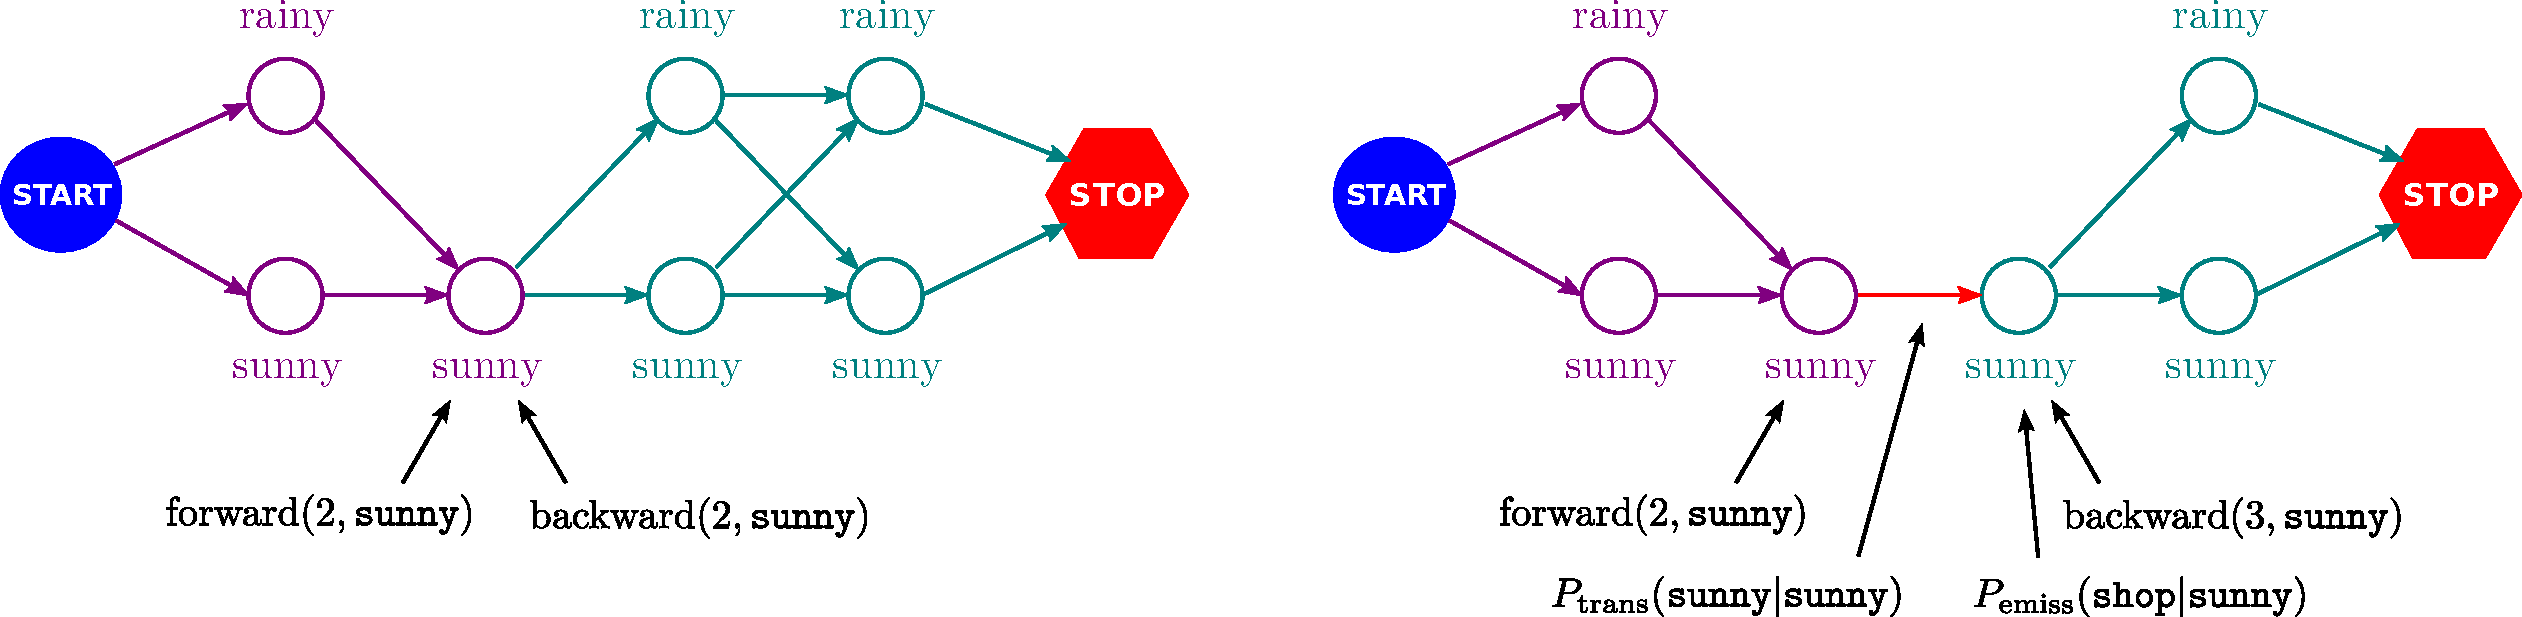
\includegraphics[width=1\textwidth]{figs/sequences/posteriors}
\caption[Posterior Illustration.]{\label{fig:posteriors} A graphical representation of the components in the state and transition posteriors. Recall that the observation sequence is ``\texttt{walk walk shop clean}''.}
\end{center}
\end{figure}

%\begin{figure}
%\begin{center}
%\begin{tabular}{cc}
%
%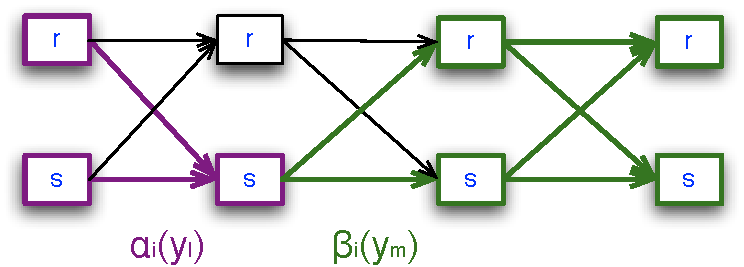
\includegraphics[scale=.5]{figs/sequences/statePost}
%& 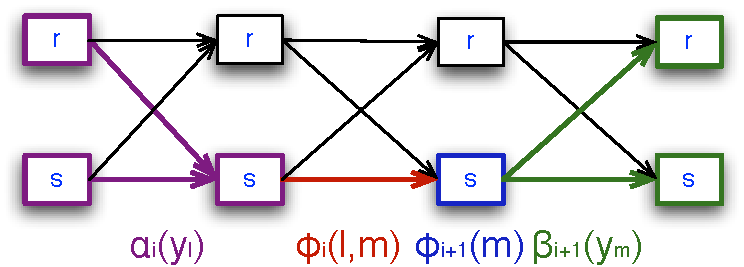
\includegraphics[scale=.5]{figs/sequences/transPost}\\
%\end{tabular}
%\caption[Posterior Illustration.]{\label{fig:posteriors} A graphical representation of the components in the state and transition posteriors.}
%
%\end{center}
%\end{figure}

Using the state posteriors, we are ready to perform posterior
decoding. 
The strategy is to compute the state posteriors 
for each position $i \in \{1,\ldots,N\}$
and each state $c_k \in \statevocab$, and 
then pick the arg-max at each position:
\begin{equation}
{\widehat y_i} := \argmax_{y_i \in \statevocab} P(Y_i=y_i| X=x).
\end{equation}

%Algorithm \ref{alg:pd} shows the posterior decoding algorithm.

%\begin{algorithm}[t]
%   \caption{Posterior Decoding algorithm \label{alg:pd}}
%\begin{algorithmic}[1]
%   \STATE {\bfseries input:} The forward and backward probabilities
%       $\alpha$ and $\beta$.
%   \STATE  \emph{Compute Likelihood}: Compute the likelihood of the
%   sentence
%   \STATE $L = 0$
%   \FOR{$\hv_l \in \hvocab$ }
%   \STATE $\marginal = \marginal + \alpha_N(\hv_l)$
%   \ENDFOR 
%   \STATE $\hat \hseq = []$
%    \FOR{$i=1$ {\bfseries to} $N$}
%    \STATE $max = 0$
%     \FOR{$\hv_l \in \hvocab$ }
%     \STATE $\gamma_i(\hv_l)  =  \frac{\alpha_i(\hv_l)
%       \beta_i(\hv_l)}{\marginal}$
%     \IF {$\gamma_i(\hv_l) > max$}
%     \STATE $max = \gamma_i(\hv_l)$
%     \STATE $\hat  y_i = \hv_l$
%     \ENDIF
%     \ENDFOR 
%     \ENDFOR 
%   \STATE \textbf{output:} the posterior path $\hat \hseq$
%\end{algorithmic}
%\end{algorithm}


\newpage
\begin{exercise}
%Given the node and edge posterior formulas \ref{eq::nodePosterior},\ref{eq::edgePosterior} and the
%  forward and backward formulas \ref{eq::forward},\ref{eq::backward}, convince yourself that formulas
%  \ref{eq::nodePosterior2},\ref{eq::edgePosterior2} are correct. 

Compute the node posteriors for the first training sequence (use the provided \emph{compute\_posteriors} function), and look at
the output. Note that the state posteriors are a proper
probability distribution (the lines of the result sum to 1).

\begin{python}
initial_scores, transition_scores, final_scores, emission_scores = hmm.compute_scores(simple.train.seq_list[0])
state_posteriors, _, _ = hmm.compute_posteriors(initial_scores,
                                                transition_scores,
                                                final_scores,
                                                emission_scores)
print state_posteriors

[[ 0.95738152  0.04261848]
 [ 0.75281282  0.24718718]
 [ 0.26184794  0.73815206]
 [ 0.          1.        ]]
\end{python}
\end{exercise}

\begin{exercise}
Run the posterior decode on the first test sequence, and evaluate it.
\begin{python}
y_pred = hmm.posterior_decode(simple.test.seq_list[0])
print "Prediction test 0:", y_pred

walk/rainy walk/rainy shop/sunny clean/sunny

print "Truth test 0:", simple.test.seq_list[0]

walk/rainy walk/sunny shop/sunny clean/sunny 
\end{python}

Do the same for the second test sequence:
\begin{python}
y_pred = hmm.posterior_decode(simple.test.seq_list[1])
print "Prediction test 1:", y_pred

clean/rainy walk/rainy tennis/rainy walk/rainy 

print "Truth test 1:", simple.test.seq_list[1]

clean/sunny walk/sunny tennis/sunny walk/sunny 
\end{python}

What is wrong? Note the observations for the second test sequence: the
observation {\tt tennis} was never seen at training time, so the probability for
it will be zero (no matter what state). This will make all possible state
sequences have zero probability.
As seen in the previous lecture, this is a problem with generative
models, which can be corrected using smoothing (among other
options).

Change the \emph{train\_supervised} method to add smoothing:
\begin{python}
def train_supervised(self,sequence_list, smoothing):
\end{python}

Try, for example, adding 0.1 to all the counts, and repeating this exercise with that smoothing. What do you observe?
\begin{python}
hmm.train_supervised(simple.train, smoothing=0.1)
y_pred = hmm.posterior_decode(simple.test.seq_list[0])
print "Prediction test 0 with smoothing:", y_pred

walk/rainy walk/rainy shop/sunny clean/sunny 

print "Truth test 0:", simple.test.seq_list[0]

walk/rainy walk/sunny shop/sunny clean/sunny

y_pred = hmm.posterior_decode(simple.test.seq_list[1])
print "Prediction test 1 with smoothing:", y_pred

clean/sunny walk/sunny tennis/sunny walk/sunny 

print "Truth test 1:", simple.test.seq_list[1]

clean/sunny walk/sunny tennis/sunny walk/sunny 
\end{python}
\end{exercise}

%Note that if you use smoothing when training, the sanity checks mentioned at the start of this chapter are no longer true. For example, the sum of all the transition counts is no longer equal to the number of tokens -- it is larger.

%\begin{exercise}
%Change the function you just created \emph{ def
%  sanity\_check\_counts(self,seq\_list):} to account for smoothing. Make
%sure it works properly.
%
%\begin{python}
%In []: run sequences/hmm.py
%In []: hmm = HMM(simple)
%In []: hmm.collect_counts_from_corpus(simple.train,smoothing=0.1)
%In []: hmm.sanity_check_counts(simple.train,smoothing=0.1)
%Init Counts match
%Final Counts match
%Transition Counts match
%Observations Counts match
%\end{python}
%\end{exercise}


\subsection{Viterbi Decoding}\label{viterbi}


\textbf{Viterbi decoding} consists in
picking the best global hidden state sequence 
$\widehat{y}$
as follows: 
\begin{equation}
\widehat{y} = \argmax_{y \in \statevocab^N} P(Y=y|X=x) = \argmax_{y \in \statevocab^N} P(X=x,Y=y).
\end{equation}

The Viterbi algorithm 
is very similar to the forward procedure of the FB algorithm,
making use of the same trellis structure to efficiently represent the exponential number of sequences without prohibitive computation costs. In fact, the only
difference from the forward-backward algorithm is in the recursion
\ref{forwardRecursion} where instead of \emph{summing} over all possible 
hidden states, we take their \emph{maximum}.

\begin{equation}
\label{eq::viterbi}
\mathbf{Viterbi }\;\;\;\;  \mathrm{viterbi}(i, y_i) = \max_{y_1...y_{i-1}} P(Y_1=y_1,\ldots Y_i = y_i , X_1=x_1,\ldots, X_i=x_i)
\end{equation}
The Viterbi trellis represents the path with maximum probability in
position
$i$ when we are in state $Y_i=y_i$ and that we have observed $x_1,\ldots,x_i$
up to that position. The Viterbi algorithm is defined by the
following recurrence: 
\begin{eqnarray}
\mathrm{viterbi}(1, c_k) &=& P_{\mathrm{init}}(c_k|\text{\tt start}) \times 
P_{\mathrm{emiss}}(x_1 | c_k)
 \\
 \mathrm{viterbi}(i, c_k) &=& \left( \displaystyle \max_{c_l \in \statevocab} P_{\mathrm{trans}}(c_k | c_l) \times \mathrm{viterbi}(i-1, c_l) \right) \times P_{\mathrm{emiss}}(x_i | c_k)  \label{viterbiRecursion}
 \\
 \mathrm{backtrack}(i, c_k) &=& \left( \displaystyle \argmax_{c_l \in \statevocab} P_{\mathrm{trans}}(c_k | c_l) \times \mathrm{viterbi}(i-1, c_l) \right) 
 \\
  \mathrm{viterbi}(N+1, \text{\tt stop}) &=& \max_{c_l \in \statevocab} P_{\mathrm{final}}(\text{\tt stop} | c_l) \times \mathrm{viterbi}(N, c_l)
 \\
  \mathrm{backtrack}(N+1, \text{\tt stop}) &=& \argmax_{c_l \in \statevocab} P_{\mathrm{final}}(\text{\tt stop} | c_l) \times \mathrm{viterbi}(N, c_l).
\end{eqnarray}


%\begin{eqnarray}
%\delta_1(\hv_l) &=& \phi_1(l) \\
%\delta_i(\hv_l) &=& \left[ \max_{y_1 ... y_i} \phi_{i-1,i}(m,l)
%  \delta_{i-1}(\hv_m) \right] \phi_i(l) \label{viterbiRecursion} \\
%\psi_{i}(\hv_l) &=& \left[ \argmax_{y_1 ... y_i} \phi_{i-1,i}(m,l)
%  \delta_{i-1}(\hv_m) \right]
%%\phi_{(i-1)}(m,l)  \delta_{i-1}(\hv_m) \right] \phi_i(l) \label{viterbiBackpointers}
%\end{eqnarray}

Algorithm \ref{alg:viterbi} shows the pseudo code for the Viterbi algorithm.
Note the similarity with the forward algorithm.
The only differences are:
\begin{itemize}
\item Maximizing instead of summing;
\item Keeping the argmax's to backtrack.
\end{itemize}

%\begin{algorithm}[t]
%   \caption{Viterbi algorithm \label{alg:viterbi}}
%\begin{algorithmic}[1]
%   \STATE {\bfseries input:} sentence $\sent$, parameters $\theta$
%        \STATE  \emph{Forward pass}: compute the maximum paths for
%        every end state
%        \STATE \emph{Initialization}
%        \FOR{$\hv_l \in \hvocab$ }
%        \STATE $\delta_1(\hv_l) = \phi_1(\hv_l)$
%        \ENDFOR 
%        \FOR{$i=2$ {\bfseries to} $N$}
%         \FOR{$\hv_l \in \hvocab$ }
%                 \STATE $\delta_i(\hv_l) = \left[ \displaystyle
%                   \max_{m  \in \hvocab} \phi_{i-1,i}(m,l)
%                   \delta_{i-1}(\hv_m) \right] \phi_i(l)$
%                 \STATE $\psi_{i}(\hv_l) = m$
%         \ENDFOR 
%        \ENDFOR 
%       %\STATE \emph{Terminate}:
%       \STATE 
%  $\max_{y \in \statevocab^N} P(X=x,Y=y) := \max_{c_l \in \statevocab} P_{\mathrm{final}}(\text{\tt stop} | c_l) \times \mathrm{viterbi}(N, c_l)$
%  	   \STATE 
%       \STATE \emph{Backward pass}: Build the most likely path
%	  \STATE $\widehat{y}_i = \argmax_{c_l \in \statevocab} P_{\mathrm{final}}(\text{\tt stop} | c_l) \times \mathrm{viterbi}(N, c_l)$ 
%	   \FOR{$i=N-1$ {\bfseries to} 1}
%        \STATE $\widehat{y_i} = \mathrm{backtrack}(i+1, \widehat{y}_{i+1})$
%        \ENDFOR 
%       \STATE \textbf{output:} the viterbi path $\widehat{y}$
%\end{algorithmic}
%\end{algorithm}

\begin{algorithm}[t]
   \caption{Viterbi algorithm \label{alg:viterbi}}
\begin{algorithmic}[1]
   \STATE {\bfseries input:} sequence $x_1,\ldots,x_N$, scores $P_{\mathrm{init}}, P_{\mathrm{trans}}, P_{\mathrm{final}}, P_{\mathrm{emiss}}$
        \STATE  \emph{Forward pass}: Compute the best paths for every end state
        \STATE \emph{Initialization}
        \FOR{$c_k \in \statevocab$ }
        \STATE $\mathrm{viterbi}(1,c_k) = P_{\mathrm{init}}(c_k|\text{\tt start}) \times 
P_{\mathrm{emiss}}(x_1 | c_k)$
        \ENDFOR 
        \FOR{$i=2$ {\bfseries to} $N$}
         \FOR{$c_k \in \statevocab$ }
          \STATE $\mathrm{viterbi}(i, c_k) = \left( \displaystyle \max_{c_l \in \statevocab} P_{\mathrm{trans}}(c_k | c_l) \times \mathrm{viterbi}(i-1, c_l) \right) \times P_{\mathrm{emiss}}(x_i | c_k)$
          \STATE $\mathrm{backtrack}(i, c_k) = \left( \displaystyle \argmax_{c_l \in \statevocab} P_{\mathrm{trans}}(c_k | c_l) \times \mathrm{viterbi}(i-1, c_l) \right)$
         \ENDFOR 
        \ENDFOR 
       \STATE 
  $\max_{y \in \statevocab^N} P(X=x,Y=y) := \max_{c_l \in \statevocab} P_{\mathrm{final}}(\text{\tt stop} | c_l) \times \mathrm{viterbi}(N, c_l)$        
        \STATE
       \STATE \emph{Backward pass}: backtrack to obtain the most likely path 
	  \STATE $\widehat{y}_N = \argmax_{c_l \in \statevocab} P_{\mathrm{final}}(\text{\tt stop} | c_l) \times \mathrm{viterbi}(N, c_l)$ 
	   \FOR{$i=N-1$ {\bfseries to} 1}
        \STATE $\widehat{y_i} = \mathrm{backtrack}(i+1, \widehat{y}_{i+1})$
        \ENDFOR 
       \STATE \textbf{output:} the viterbi path $\widehat{y}$.
\end{algorithmic}
\end{algorithm}

\section{Assignment}

With the previous theoretical background, you have the necessary tools to solve today's assignment.

\begin{exercise}
Implement a method 
for performing Viterbi decoding in 
file {\tt sequence\_classification\_decoder.py}.
\begin{python}
        def run_viterbi(self, initial_scores, transition_scores, final_scores, emission_scores):
\end{python}
Hint: look at the implementation of {\tt run\_forward}. Also check the help for the numpy methods max and argmax.

This method will be called 
by 
\begin{python}
def viterbi_decode(self, sequence)
\end{python}
in the module {\tt sequence\_classifier.py}.
%
%posterior decoding (the function \emph{posterior\_decode}) for reference.

Test your method on both test sequences and compare the results with
the ones given.
\begin{python}
hmm.train_supervised(simple.train, smoothing=0.1)
y_pred, score = hmm.viterbi_decode(simple.test.seq_list[0])
print "Viterbi decoding Prediction test 0 with smoothing:", y_pred, score

walk/rainy walk/rainy shop/sunny clean/sunny  -6.02050124698

print "Truth test 0:", simple.test.seq_list[0]

walk/rainy walk/sunny shop/sunny clean/sunny 

y_pred, score = hmm.viterbi_decode(simple.test.seq_list[1])
print "Viterbi decoding Prediction test 1 with smoothing:", y_pred, score

clean/sunny walk/sunny tennis/sunny walk/sunny  -11.713974074

print "Truth test 1:", simple.test.seq_list[1]

clean/sunny walk/sunny tennis/sunny walk/sunny 
\end{python}

Note: since we didn't run the \emph{train\_supervised} method again, we are still using the result of the training using smoothing. Therefore, you should compare these results to the ones of posterior decoding with smoothing.

\end{exercise}




%%% Local Variables: 
%%% mode: latex
%%% TeX-master: "../../guide"
%%% End: 


\section{\label{pos-tagging} Part-of-Speech Tagging (POS)}
Part-of-Speech (PoS) tagging is one of the most important NLP tasks. The
task is to assign each word a grammatical category, or Part-of-Speech, \emph{i.e.} noun,
verb, adjective,... Recalling the defined notation, $\vocab$ is a 
vocabulary of word types, and 
$\statevocab$ is the set of Part-of-Speech tags.

In English, using the Penn Treebank (PTB) corpus \citep{pennTreeBank}, the current
state of the art for part of speech tagging is around 97\% for a
variety of methods.

In the rest of this class we will use a subset of the PTB corpus, but
instead of using the original 45 tags we will use a reduced tag set of
12 tags, to make the algorithms faster for the
class. In this task, $x$ is a sentence (\emph{i.e.}, a sequence of word tokens) and $y$
is the sequence of possible PoS tags.

The first step is to load the corpus. We will start by loading
1000 sentences for training and 1000 sentences both for development and
testing. Then we train the HMM model by maximum likelihood estimation.
\begin{python}
import lxmls.readers.pos_corpus as pcc
corpus = pcc.PostagCorpus()
train_seq = corpus.read_sequence_list_conll("data/train-02-21.conll",max_sent_len=15,max_nr_sent=1000)
test_seq = corpus.read_sequence_list_conll("data/test-23.conll",max_sent_len=15,max_nr_sent=1000)
dev_seq = corpus.read_sequence_list_conll("data/dev-22.conll",max_sent_len=15,max_nr_sent=1000)
hmm = hmmc.HMM(corpus.word_dict, corpus.tag_dict)
hmm.train_supervised(train_seq)
hmm.print_transition_matrix()
\end{python}


Look at the transition probabilities of the trained model
%\begin{python}
%In []: import matplotlib.pyplot as plt
%In []: hmm.transition_probs
%\end{python}
 (see
Figure \ref{fig:transProbs}), and see if they match your intuition
about the English language (e.g. adjectives tend to come before nouns).

\begin{figure}[h!]
\centering
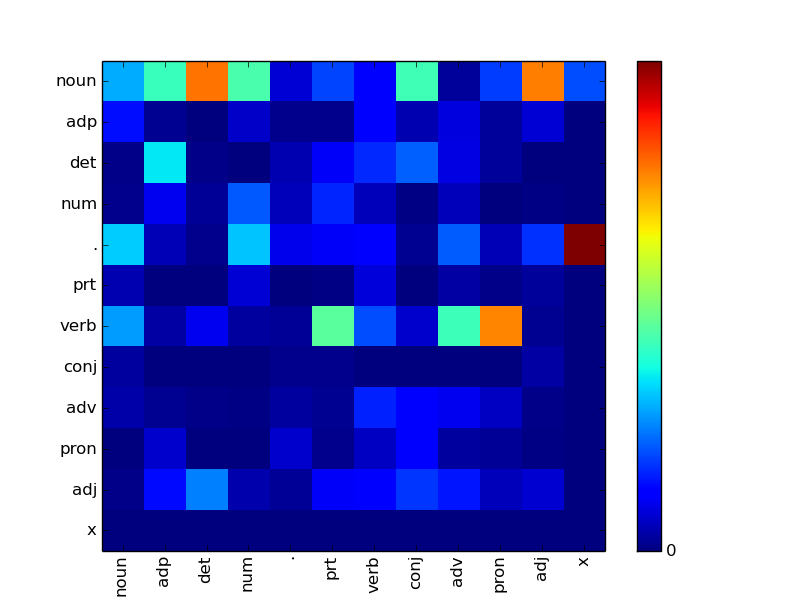
\includegraphics[scale=.5]{figs/sequences/transition_probs}
\caption{\label{fig:transProbs} Transition probabilities of the
trained model. Each column is the previous state and row is the current
state. Note the high probability of having Noun after Determinant or Adjective, or of having Verb after Nouns or Pronouns, as expected.}
\end{figure}

\begin{exercise}
Test the model using both posterior decoding and Viterbi decoding on
both the train and test set, using the methods in class HMM:
\begin{python}
viterbi_pred_train = hmm.viterbi_decode_corpus(train_seq)
posterior_pred_train = hmm.posterior_decode_corpus(train_seq)
eval_viterbi_train =   hmm.evaluate_corpus(train_seq, viterbi_pred_train)
eval_posterior_train =  hmm.evaluate_corpus(train_seq, posterior_pred_train)
print "Train Set Accuracy: Posterior Decode \%.3f, Viterbi Decode: \%.3f"\%(eval_posterior_train,eval_viterbi_train)

Train Set Accuracy: Posterior Decode 0.985, Viterbi Decode: 0.985

viterbi_pred_test = hmm.viterbi_decode_corpus(test_seq)
posterior_pred_test = hmm.posterior_decode_corpus(test_seq)
eval_viterbi_test =   hmm.evaluate_corpus(test_seq,viterbi_pred_test)
eval_posterior_test = hmm.evaluate_corpus(test_seq,posterior_pred_test)
print "Test Set Accuracy: Posterior Decode \%.3f, Viterbi Decode: \%.3f"\%(eval_posterior_test,eval_viterbi_test)

Test Set Accuracy: Posterior Decode 0.350, Viterbi Decode: 0.509
\end{python}
What do you observe? Remake the previous exercise but now train the HMM
using smoothing. Try different values (0,0.1,0.01,1) and report the results on the
train and development set. (Use function
\emph{pick\_best\_smoothing}).


\begin{python}
best_smoothing = hmm.pick_best_smoothing(train_seq, dev_seq, [10,1,0.1,0])

Smoothing 10.000000 --  Train Set Accuracy: Posterior Decode 0.731, Viterbi Decode: 0.691
Smoothing 10.000000 -- Test Set Accuracy: Posterior Decode 0.712, Viterbi Decode: 0.675
Smoothing 1.000000 --  Train Set Accuracy: Posterior Decode 0.887, Viterbi Decode: 0.865
Smoothing 1.000000 -- Test Set Accuracy: Posterior Decode 0.818, Viterbi Decode: 0.792
Smoothing 0.100000 --  Train Set Accuracy: Posterior Decode 0.968, Viterbi Decode: 0.965
Smoothing 0.100000 -- Test Set Accuracy: Posterior Decode 0.851, Viterbi Decode: 0.842
Smoothing 0.000000 --  Train Set Accuracy: Posterior Decode 0.985, Viterbi Decode: 0.985
Smoothing 0.000000 -- Test Set Accuracy: Posterior Decode 0.370, Viterbi Decode: 0.526

hmm.train_supervised(train_seq, smoothing=best_smoothing)
viterbi_pred_test = hmm.viterbi_decode_corpus(test_seq)
posterior_pred_test = hmm.posterior_decode_corpus(test_seq)
eval_viterbi_test =   hmm.evaluate_corpus(test_seq, viterbi_pred_test)
eval_posterior_test = hmm.evaluate_corpus(test_seq, posterior_pred_test)
print "Best Smoothing \%f --  Test Set Accuracy: Posterior Decode \%.3f, Viterbi Decode: \%.3f"%(best_smoothing,eval_posterior_test,eval_viterbi_test)

Best Smoothing 0.100000 --  Test Set Accuracy: Posterior Decode 0.837, Viterbi Decode: 0.827
\end{python}


Perform some error analysis to understand were the errors are coming
from. You can start by visualizing the confusion matrix (true tags vs
predicted tags). You should get something like what is shown in Figure~\ref{fig:cmuns}.

\begin{python}
import lxmls.sequences.confusion_matrix as cm
import matplotlib.pyplot as plt
confusion_matrix = cm.build_confusion_matrix(test_seq.seq_list, viterbi_pred_test, len(corpus.tag_dict), hmm.get_num_states())
cm.plot_confusion_bar_graph(confusion_matrix, corpus.tag_dict, xrange(hmm.get_num_states()), 'Confusion matrix')
plt.show()
\end{python}

\begin{figure}[h!]
\centering
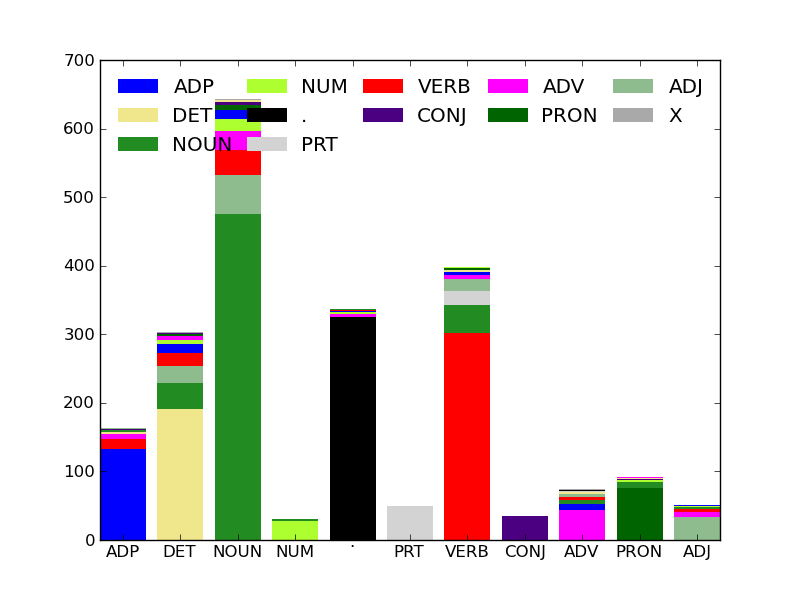
\includegraphics[scale=.4]{figs/sequences/cm_sup.png}
\caption{\label{fig:cmuns} Confusion Matrix for the previous
  example. Predicted tags are columns and the true tags corresponds to
  the constituents of each column.}
\end{figure}

\end{exercise}


%\begin{exercise}
%Implement a function that produces the accuracy for rare words vs
%common words. Use you own definition of rare word.
%
%Can you come up with other error analysis methods? Which?
%
%\end{exercise}

%\begin{exercise}
%So far we have only worked with a limited dataset of 1000 words. Try increasing the number of sentences to 10000. What do you observe?
%\end{exercise}


%\section{Unsupervised Learning of HMMs}
%
%\afm{explain here the EM algorithm}
%
%\begin{python}
%
%Initial accuracy: 0.303638
%Iter: 1 Log Likelihood: -101824.763927
%Iter: 1 Accuracy: 0.305441
%Iter: 2 Log Likelihood: -78057.108346
%Iter: 2 Accuracy: 0.321976
%Iter: 3 Log Likelihood: -77813.725501
%Iter: 3 Accuracy: 0.357451
%Iter: 4 Log Likelihood: -77192.947674
%Iter: 4 Accuracy: 0.385109
%Iter: 5 Log Likelihood: -76191.800849
%Iter: 5 Accuracy: 0.392123
%Iter: 6 Log Likelihood: -75242.572729
%Iter: 6 Accuracy: 0.391121
%Iter: 7 Log Likelihood: -74392.892496
%Iter: 7 Accuracy: 0.404249
%Iter: 8 Log Likelihood: -73357.542833
%Iter: 8 Accuracy: 0.399940
%Iter: 9 Log Likelihood: -72135.182778
%Iter: 9 Accuracy: 0.399238
%Iter: 10 Log Likelihood: -70924.246230
%Iter: 10 Accuracy: 0.395430
%Iter: 11 Log Likelihood: -69906.561800
%Iter: 11 Accuracy: 0.394328
%Iter: 12 Log Likelihood: -69140.228623
%Iter: 12 Accuracy: 0.390821
%Iter: 13 Log Likelihood: -68541.416423
%Iter: 13 Accuracy: 0.391522
%Iter: 14 Log Likelihood: -68053.456865
%Iter: 14 Accuracy: 0.389117
%Iter: 15 Log Likelihood: -67667.318961
%Iter: 15 Accuracy: 0.386411
%Iter: 16 Log Likelihood: -67337.685686
%Iter: 16 Accuracy: 0.385409
%Iter: 17 Log Likelihood: -67054.571821
%Iter: 17 Accuracy: 0.385409
%Iter: 18 Log Likelihood: -66769.973881
%Iter: 18 Accuracy: 0.385409
%Iter: 19 Log Likelihood: -66442.608458
%Iter: 19 Accuracy: 0.385409
%
%\end{python}



%\section{\label{hmm_special_state} HMM Initial and Final State}
%\input{pages/sequences/init_final_hmm.tex}

%\section{\label{hmm} Second order HMM}
%
\subsection{State Expansion}

The ideia here is to expand the states and use the same inference
procedures as those of the HMM.



\subsection{Modelling second order}

Here we use the original states and we derive new inference procedures....

\begin{eqnarray*}
\alpha_{t=2}(1) &=& P(y_{t=2} = 1,x_0,x_1,x_2) = \sum_{b \in \hvocab}
\sum_{a\in \hvocab} P(y_{t=2} = 1,x_0,x_1,x_2, y_{t=0}=a,y_{t=1}=b)\\
\alpha_{t=2}(1) &=& \sum_{b \in \hvocab}
\sum_{a\in \hvocab}
p(x_2 |  y_{t=2}) p(y_{t=2} | y_{t=1} =b ,y_{t=0}=a)  p(x_1 |  y_{t=1}
=b) p(y_{t=1} =b| y_{t=0}=a)\\
&*&  p(x_0 |  y_{t=0}=a) p(y_{t=0}=a) \\
\alpha_{t=2}(1) &=& \sum_{b \in \hvocab}
\sum_{a\in \hvocab}
p(x_2 |  y_{t=2}) p(y_{t=2} | y_{t=1} = b,y_{t=0} = a)  p(x_1 |
y_{t=1} = b) p(y_{t=1} = b| y_{t=0} = a)  \mathbf{p(x_0 ,  y_{t=0} = a) }\\
\alpha_{t=2}(1) &=& \sum_{b \in \hvocab}
\sum_{a\in \hvocab}
p(x_2 |  y_{t=2}) p(y_{t=2} | y_{t=1} = b,y_{t=0} = a)  p(x_1 |
y_{t=1} = b) p(y_{t=1} = b| y_{t=0} = a)  \alpha_{t=0}(a) \\
\alpha_{t=2}(1) &=& \sum_{b \in \hvocab}
\sum_{a\in \hvocab}
p(x_2 |  y_{t=2}) p(y_{t=2} | y_{t=1} = b,y_{t=0} = a)  p(x_1 ,
y_{t=1} = b | y_{t=0} = a)  \alpha_{t=0}(a) \\
\alpha_{t=2}(1) &=& \sum_{b \in \hvocab}
\sum_{a\in \hvocab}
p(x_2 |  y_{t=2}) p(y_{t=2} | y_{t=1} = b,y_{t=0} = a)  \mathbf{p(x_1 ,
y_{t=1} = b ,x_0 ,  y_{t=0} = a) }
\end{eqnarray*}

%%% Local Variables: 
%%% mode: latex
%%% TeX-master: "../../guide"
%%% End: 


%%% Local Variables: 
%%% mode: latex
%%% TeX-master: "../../guide.tex"
%%% End: 


\chapter{Non-Linear Classifiers}
\section{Today's assignment}
Today's class will be divided in two main parts. Firstly, we will learn about
computation graphs and the Backpropagation algorithm. We will also code
Backpropagation in Numpy for a simple model (a feed forward network). Secondly,
we will learn the basics of the Theano module for Python. Theano allows you to
implement  generic computation graphs, automatically compute gradients with
respect to their parameters and make use of Graphical Processing Units (GPUs)
for optimal speed. 

If you are new to the topic, you should aim to understand the concept of computation graph, 
finish the Backpropagation exercise and attain a basic understanding of Theano.
If you already know Backpropagation well and have experience with normal
Python, you should aim to complete the whole day. 

\section{Introduction to Deep Learning and Theano}

Deep learning is the name behind the latest wave of neural network research.
This is a very old topic, dating from the first half of the 20th century, that
has attained formidable impact in the machine learning community recently. 
There is nothing particularly difficult in deep learning. You have already
visited all the mathematical principles you need in the first days of the
labs of this school. At their core, deep learning models are just functions
mapping vector inputs $\mathbf{x}$ to vector outputs $\mathbf{y}$, constructed by
composing linear and non-linear functions. This composition can be expressed in
the form of a \textit{computation graph}, where each node applies a function to
its inputs and passes the result as its output. The parameters of the model are
the weights given to the different inputs in nodes applying linear
functions. This vaguely resembles synapse strengths in human neural networks,
hence the name artificial neural networks. 

Due to their compositional nature, gradient methods and the chain rule can be
applied learn the parameters of these models regardless of their complexity.
See Section \label{gradient_methods} for a refresh on the basic concept. We
will also refer to the gradient learning methods introduced in Section
\ref{s:me}. Today we will focus on \textit{feed-forward networks}. Tomorrow we will
extended today's class to \textit{recurrent neural networks} (RNNs).  

Some of the changes that led to the surge of deep learning are not only
improvements on the existing neural network algorithms, but also
the increase in the amount of data available and computing power. In
particular, the use of Graphical Processing Units (GPUs) has allowed neural
networks to be applied to very large datasets. Working with GPUs is not trivial
as it requires dealing with specialized hardware. Luckily, as it is often the
case, we are one Python import away from solving this problem. 

For the particular case of deep learning, there is a growing number of python
toolboxes available that allow you to design custom computational graphs for
GPUs as e.g.
Theano\footnotemark\footnotetext{http://deeplearning.net/software/theano/} or TensorFlow\footnotemark\footnotetext{https://www.tensorflow.org/}.

In these labs we will be working with Theano. Theano allows us to express
computation graphs symbolically in terms of basic algebraic operations. It also
automatically computes gradients and produces CUDA-compatible code for GPUs. The
exercises are designed to gain a low-level understanding of Theano. If you are
only looking forward to utilize pre-designed models, the Keras
toolbox\footnotemark\footnotetext{http://keras.io/} provides high-level
operations compatible with both Theano and TensorFlow. 

\section{Computation Graphs} 

\subsection{Example: The computation graph of a log-linear model}

\begin{figure}[!h]
\centering
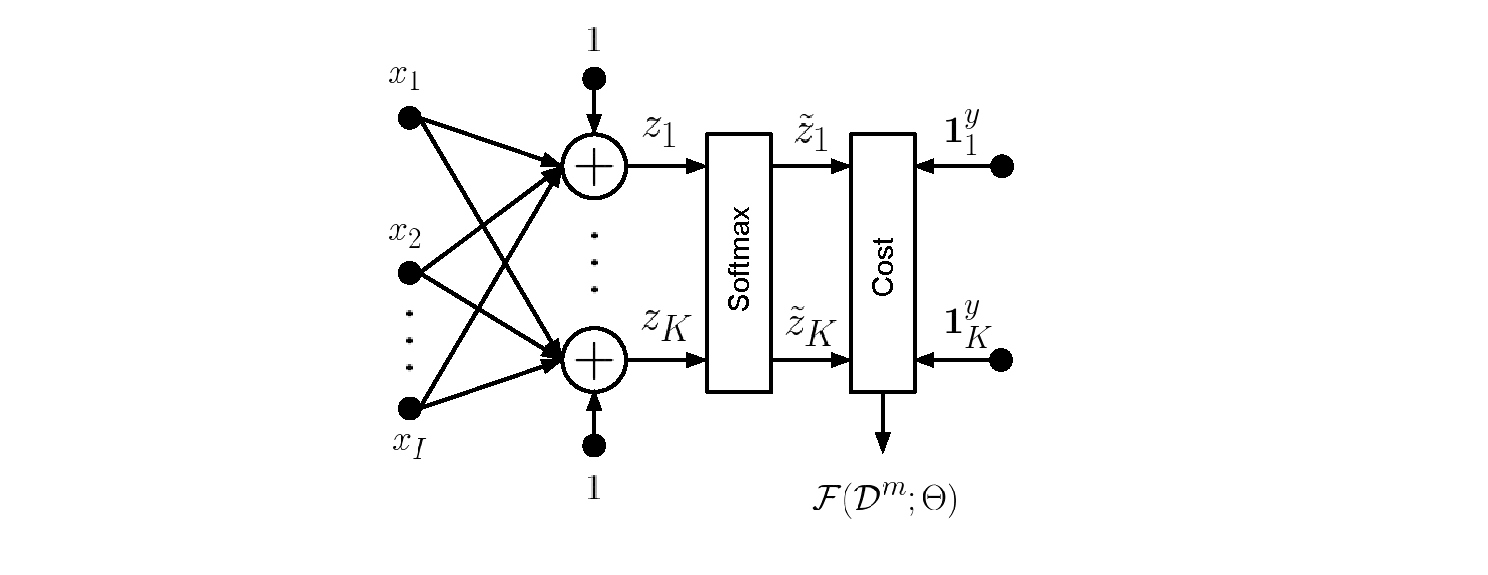
\includegraphics[scale=0.6]{figs/deep_learning/LogLin.pdf}
\caption{Representation of a log-linear model as a computation graph: a
composition of linear and non-linear transformations. The classification cost
for the $m$-th training example $\mathcal{D}^m=\{\mathbf{x}, y\}$ is also
shown. Note $\mathbf{1}^y$ is an indicator vector with a one in position $y$.} 
\label{fig:LogLinear}
\end{figure}

A computation graph is just a way of expressing a multi-input multi-output
function with a directed acyclic graph. Each node in the graph applies a
function over the outputs of its parent nodes and passes the result to its child-nodes,
thus attaining very complex functions by \textit{composing} simpler functions.
To introduce the concept we will work with a very simple example, a categorical
distribution over $K$ classes parametrized as a log-linear model. This is given
by
%
\begin{align}
p(y=k|{x}) & = \frac{1}{Z(\mathbf{W},\mathbf{b},\mathbf{x})}\exp\left(\sum_{i=1}^{I} W_{ik} x_i + b_k\right),
\label{eq:loglineargen}
\end{align}
%
\noindent where 
\begin{align}
Z(\mathbf{W},\mathbf{b},\mathbf{x}) = \sum_{k'=1}^{K} \exp\left(\sum_{i=1}^{I} W_{ik'} x_i + b_{k'}\right)
\label{eq:loglineargenPartition}
\end{align}
%
is the partition function ensuring that all output values sum to one, so that we can interpret
these values as probabilities. The model thus receives a feature vector
$\mathbf{x} \in \mathbb{R}^{I}$ and assigns a probability over $y \in {1 \cdots K}$ possible
class indices. It is parametrized by weights and bias $\Theta=\{\mathbf{W},
\mathbf{b}\}$, with $\mathbf{W} \in \mathbb{R}^{K \times J}$ and $\mathbf{b}
\in \mathbb{R}^{K}$. This is a well known classifier bearing resemblance to the
models seen in the second day of the school, in
particular the maxent model\footnotemark\footnotetext{There are some
differences with respect to Eq.\ref{eq:loglinear}, like the use of a bias
$\mathbf{b}$. Also, if we consider the binary joint feature mapping
$\boldsymbol{f}(x,y) = \boldsymbol{g}(x) \otimes \boldsymbol{e}_y\nonumber$ of
Eq.\ref{eq:jointfeatsimple}, the maximum entropy classifier in
Eq.\ref{eq:loglinear} becomes a special case of Eq.\ref{eq:loglineargen}, in
which the feature vector $\mathbf{x}$ only take binary values and the bias
parameters in $\mathbf{b}$ are all set to zero.}. 

Another way of looking at these models is as the composition of the linear transformation 
%
\begin{equation}
    z_k = \sum_{i=1}^{I} W_{ik} x_i + b_k,
\label{eq:linear}
\end{equation}
%\begin{equation}
%\mathbf{z} = \mathbf{W} \cdot \mathbf{x} + \mathbf{b},
%\label{eq:linear}
%\end{equation}
%
with the \textit{softmax} non-linear transformation

\begin{equation}
p(y=k|{x}) \equiv \tilde{z}_k = \frac{\exp(z_k)}{\sum_{k'=1}^{K} \exp(z_{k'})}.
\label{eq:softmax}
\end{equation}

This is shown as a computation graph in Fig.~\ref{fig:LogLinear}. Note that in
the following sections we will also use $\mathbf{z}$ and $\tilde{\mathbf{z}}$
to denote the output of linear and non-linear functions respectively.

\subsection{Stochastic Gradient Descent: a refresher}

As we saw on day one, the parameters of a log linear model
$\Theta=\{\mathbf{W}, \mathbf{b}\}$ can be learned with Stochastic Gradient Descent (SGD). To apply SGD we first need to define an error function that measures how
good we are doing for any given parameter values. %.
 To remain close to the maximum
entropy example, we will use as cost function the average minus posterior probability of
the correct class, also known as the Cross-Entropy (CE) criterion. Bear in
mind, however, that we could pick other non-linear functions and cost functions
that do not have
a probabilistic interpretation. For example, the same principle could be applied to
a regression problem where the cost is the Mean Square Error (MSE).

For a training data-set $\mathcal{D} = \{(\mathbf{x}^1,y^1), \ldots,
(\mathbf{x}^M,y^M)\}$ of $M$ examples, the CE cost function is given by

\begin{align}
\mathcal{F}(\mathcal{D};\Theta) 
& = -\frac{1}{M}\sum_{m=1}^{M} \log p(y^m=k(m) | \mathbf{x}^m),
\label{eq:CostLogPos}
\end{align}
% \nonumber\\&= -\frac{1}{M}\sum_{m=0}^{M-1} (\log \circ f_{k(m)} \circ \mathbf{g})(\mathbf{x}^m^)
%
where $k(m)$ is the correct class index for the $m$-th example.
To learn the parameters of this model with SGD, all we need to do is compute the gradient
of the cost $\nabla\mathcal{F}$ with respect to the parameters of the model and
iteratively update our  parameter estimates as 

\begin{equation}
\mathbf{W} \leftarrow \mathbf{W} - \eta \nabla_\mathbf{W}\mathcal{F}
\end{equation}
and
\begin{equation}
\mathbf{b} \leftarrow \mathbf{b} - \eta \nabla_\mathbf{b}\mathcal{F},
\end{equation}

\noindent where $\eta$ is the learning rate. Note that in practice we will use
a mini-batch of examples as opposed to the whole train set. Very often, more
elaborated learning rules as e.g. momentum or Adagrad are used. Bear in mind
that, in general, these still require the computation of the gradients as the
main step. The reasoning here outlined will also be applicable to these.  

\subsection{Deriving Gradients in Computation Graphs using the Chain Rule}

\begin{figure}[!h]
\centering
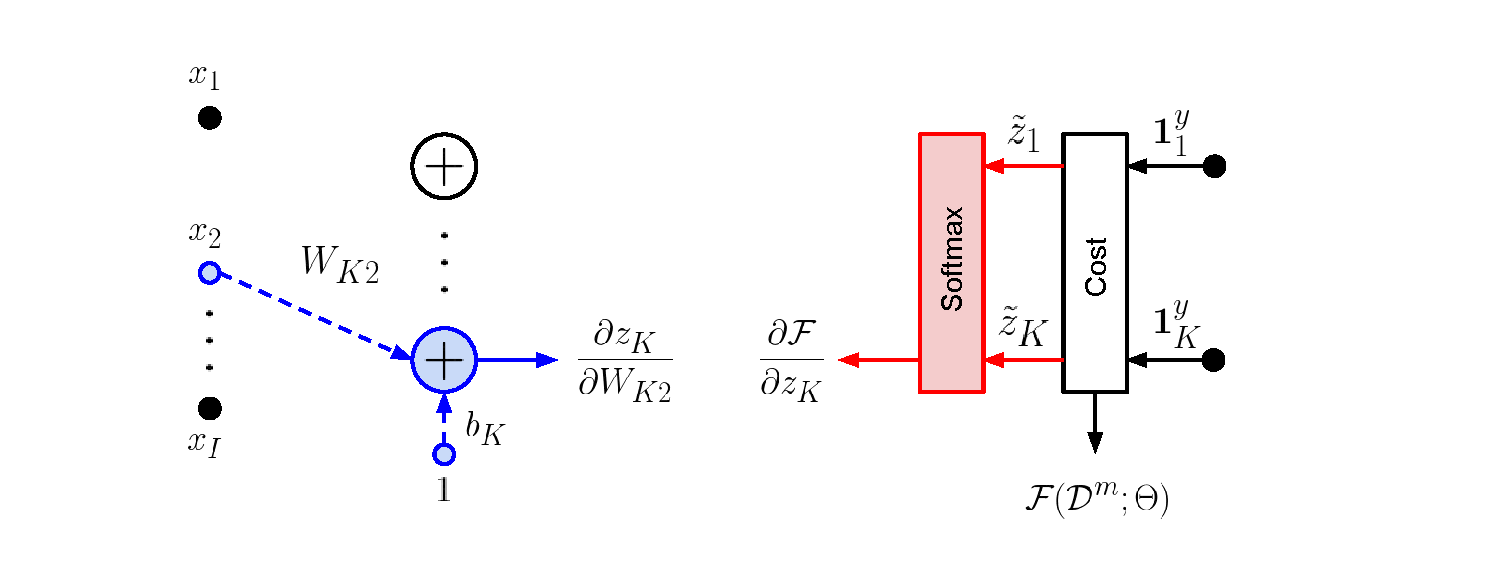
\includegraphics[scale=0.6]{figs/deep_learning/LogLin_color.pdf}
\caption{Forward-pass (blue) and Backpropagation (red) calculations to estimate the gradient of weight $W_{K2}$ and bias $b_K$ of a log-linear model.}
\label{fig:LogLinColor}
\end{figure}

The expressions for $\nabla\mathcal{F}$ are well known in the case of log-linear models. However, for
the sake of the introduction to deep learning, we will show how they can
be derived by exploiting the decomposition of the cost function into the computational
graph seen in the last section (and represented in Fig.~\ref{fig:LogLinear}). To simplify notation, and without loss of generality, we will work with the 
classification cost of an individual example 
%
\begin{align}
\mathcal{F}(\mathcal{D}^m;\Theta) 
= -\log p(y^m=k(m) | \mathbf{x}^m), 
\label{eq:CostLogPosExample}
\end{align}
%
where $\mathcal{D}^m=\{(\mathbf{x}^m, y^m)\}$. Due to linearity, extending the
gradients of Eq. \ref{eq:CostLogPosExample} to $M$ examples as in
Eq. \ref{eq:CostLogPos} simply requires computing the average of the gradients for
the individual examples. That is

% DAVID: A formula is worth a lot of words

\begin{align}
\nabla_\mathbf{W}\mathcal{F}(\mathcal{Dˆm};\Theta) = - \frac{1}{M} \sum_{m=1}^M \nabla_\mathbf{W} \log p(y^m=k(m) | \mathbf{x}^m)
\label{eq:GradientCostDecomposition}
\end{align}

All we need to do to compute $\nabla_\mathbf{W}\mathcal{F}(\mathcal{D};\Theta)$  is to have an expression for $\nabla_\mathbf{W} \log p(y^m=k(m) | \mathbf{x}^m)$.

% RAMON: This might need to be clarified
%Also in a slight abuse of notation we will denote the derivative of the cost
%with respect to an intermediate variable of the graph $z$ as
%\begin{align}
% \frac{\partial \mathcal{F}(\mathcal{D}^m;\Theta)}{\partial z}
%\end{align}

Lets start by computing the element $(k,i)$ of the gradient matrix
$\nabla_\mathbf{W}\mathcal{F}(\mathcal{Dˆm};\Theta)$, which contains the partial
derivative with respect to the weight $W_{ki}$. To do this, we invoke the \textbf{chain rule} to split the derivative calculation into two terms at variable $z_{k'}$ (Eq.\ref{eq:linear}) with $k'=1\cdots K$
%
\begin{align}
\frac{\partial \mathcal{F}(\mathcal{Dˆm};\Theta)}{\partial W_{ki}} & = \sum_{k'=1}^{K} { \color{red} \frac{\partial \mathcal{F}(\mathcal{Dˆm};\Theta)}{\partial z_{k'}} }{ \color{blue} \frac{\partial z_{k'}}{\partial W_{ki}}}.
\label{eq:LogLingCR1}
\end{align}
%
We have thus transformed the problem of computing the derivative into computing two easier derivatives. Since $z_{k'}$ only depends on the weight $W_{ki}$ in a linear way (see the graph in Fig.~\ref{fig:LogLinColor}), the second derivative in Eq.\ref{eq:LogLingCR1} is given by
\begin{align}
\frac{\partial z_{k'}}{\partial W_{ki}} = \frac{\partial }{\partial W_{ki}}\left(\sum_{i'=1}^{I} W_{k'i'} x^m_{i'} + b_{k'} \right) = 
  &\begin{cases}
      x_i^m  &  \mbox{ if } k = k'\\ 
      0    &  \mbox{ otherwise },
  \end{cases}
  \label{eq:partialLinear}
\end{align}
%
\noindent which implies that 
%
\begin{align}
\frac{\partial \mathcal{F}(\mathcal{D}^m;\Theta)}{\partial W_{ki}} = \frac{\partial \mathcal{F}(\mathcal{D}^m;\Theta) }{\partial z_k} x^m_i .
\label{eq:gradlogPycx}
\end{align}
%
\noindent The first term derivative is given by
%
\begin{align}
\frac{\partial \mathcal{F}(\mathcal{D}^m;\Theta)}{\partial z_{k}} = \frac{\partial }{\partial z_{k}}\left(z_k - \log\left(\sum_{k'=1}^{K} \exp(z_{k'}) \right) \right) = 
  \begin{cases}
      1 - \tilde{z}_k  &  \mbox{ if } k = k(m)\\ 
      -\tilde{z}_k    &  \mbox{ otherwise }.
  \end{cases}
  \label{eq:patialSoftmax}
\end{align}
%
From the formula for each element and a single example, we can now obtain the gradient matrix for a batch of $M$ examples by simply averaging and expressing the previous equations in vector form as follows
\begin{equation}
\nabla_\mathbf{W}\mathcal{F}(\mathcal{D};\Theta) = -\frac{1}{M}\sum_{m=1}^{M} \Big(\mathrm{\mathbf{1}}^{y^m} - \tilde{\mathbf{z}}^m \Big) \left(\mathbf{x}^m\right)^T.
\label{gradWeigths}
\end{equation}
%
Here $\mathrm{\mathbf{1}}^{y^m} \in \mathbb{R}^{K}$ is a vector of zeros with a one in $y^m=k(m)$, which is 
the index of the correct class for the example $m$. 

In order to compute the derivatives of the cost function with respect to the
bias parameters $b_{k}$, we only need to compute one additional derivative
\begin{align}
\frac{\partial z_{k'}}{\partial b_{k}} = 
  &\begin{cases}
      1  &  \mbox{ if } k = k'\\ 
      0  &  \mbox{ otherwise }.
  \end{cases} 
  \label{eqn:eqsilonq}
\end{align}
%
This leads us to the last gradient expression

\begin{equation}
\nabla_\mathbf{b}\mathcal{F}(\mathcal{D};\Theta) = -\frac{1}{M}\sum_{m=1}^{M} \Big(\mathrm{\mathbf{1}}^{y^m} - \tilde{\mathbf{z}}^m \Big).
\label{eq:gradBias}
\end{equation}

\noindent An important consequence of the previous derivation is the fact that each 
gradient of the parameters $\nabla_\mathbf{W}\mathcal{F}(\mathcal{D};\Theta)$ and $\nabla_\mathbf{b}\mathcal{F}(\mathcal{D};\Theta)$ can be computed from two terms: 
%
\begin{enumerate}
\item The derivative of the cost with respect to the linear transformation applying the weight $\partial \mathcal{F}(\mathcal{D}^m;\Theta)/\partial z_k$, denoted in \textcolor{red}{red}.
\item The derivative of the forward-pass up to the linear transformation applying the weight $\partial z_k/\partial W_{ik}$, denoted in \textcolor{blue}{blue}. This is always equal to the variable multiplying that weight and one in the case of the bias.
\end{enumerate}
%
\noindent This is the key to the Backpropagation algorithm as we will see in the next Section \ref{sec:deep_forward}.

\section{Going Deeper than Log-linear by using Composition}
\label{sec:deep_forward}

\subsection{The Multilayer Perceptron or Feed-Forward Network}

We have seen that just by using the chain rule we can easily compute gradients for
compositions of two functions (one non-linear and one linear). However, there
was nothing in the derivation that would stop us from composing more than two
functions. Let us think, for example of the following model

\begin{algorithm}[th!]
   \caption{Forward pass of a Multi-Layer Perceptron (MLP) or Feed-Forward (FF) network}
\begin{algorithmic}[1]
\label{algo:mlpforward}

   \STATE {\bfseries input:} Initial parameters for an MLP of $N$ layers $\Theta=\{\mathbf{W}^1, \mathbf{b}^1, \cdots \mathbf{W}^N, \mathbf{b}^N\}$
   \STATE {\bfseries input:} Input data vector $\mathbf{\tilde{z}}^{0}  \equiv \mathbf{x}$. 

	\FOR{$n=1$ {\bfseries to} $N-1$}
     \STATE Apply  linear transformation 
        $$z_j^n = \sum_{i=1}^{I} W_{ji}^n \tilde{z}_i^{n-1} + b_j^n$$
     \STATE Apply non-linear transformation e.g. sigmoid (hereby denoted $\sigma()$)
     $$\tilde{z}_j^n = \sigma(z_j^n)  = \frac{1}{1+\exp(-z_j^n)}$$

	\ENDFOR

\STATE Apply final linear transformation 
   $$z_k^N = \sum_{j=1}^{J} W_{kj}^N \tilde{z}_j^{N-1} + b_k^N$$
\STATE Apply final non-linear transformation e.g. softmax 
$$p(y=k|{x}) \equiv \tilde{z}_k^N = \frac{\exp(z_k^N)}{\sum_{k'=1}^{K} \exp(z_{k'}^N)}$$

\end{algorithmic}
\end{algorithm}

\noindent In a similar fashion to the log-linear model, the MLP/FF can be expressed as a computation graph. This is displayed in Fig.~\ref{fig:FF}

\begin{figure}[!hb]
\centering
%\includegraphics[scale=0.2]{figs/deep_learning/mlp.png}
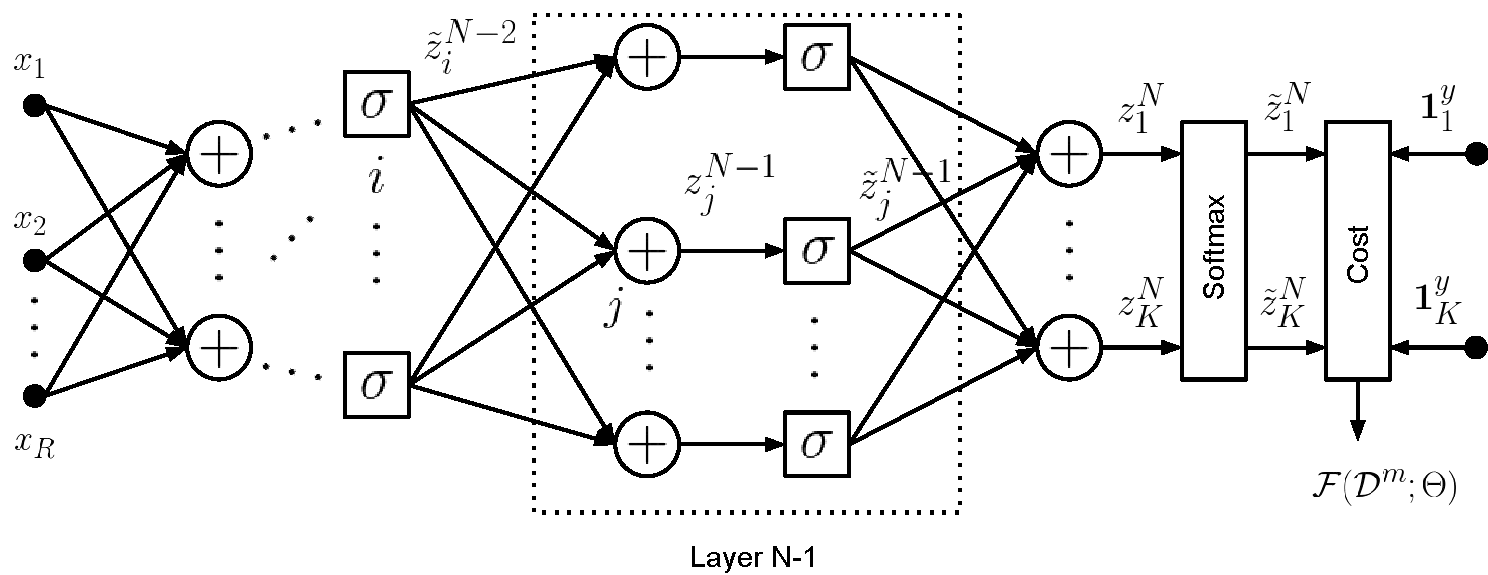
\includegraphics[scale=0.6]{figs/deep_learning/NN.pdf}
\caption{Representation of a Multi-Layer Perceptron (MLP) or Feed-Forward (FF) network as a computation graph. The classification cost
for the $m$-th training example $\mathcal{D}^m=\{\mathbf{x}, y\}$ is also
shown.}
\label{fig:FF}
\end{figure}

\noindent Some considerations:
%
\begin{itemize}
\item MLPs/FFs are characterized by applying functions in a set of layers subsequently to a single input. This characteristic is also shared by convolutional networks, although the latter also have parameter tying constraints.
\item The non-linearities in the intermediate layers are usually one-to-one transformations. The most typical are the sigmoid, hyperbolic tangent and the rectified linear unit (ReLU). 
\item The output non-linearity is determined by the output to be estimated. In order to estimate probability distributions the softmax is typically used. For regression problems a last linear layer is used instead.
\end{itemize}

\subsection{Backpropagation: an overview}

For the examples in this chapter we will consider the case in which we are estimating a distribution over classes, thus we will use the CE cost function (Eq. \ref{eq:CostLogPos}). 
% SILVIO: this is the same cost function presented earlier.

% The cost function is thus the same
% \begin{align}
% \mathcal{F}(\mathcal{D};\Theta) & = -\frac{1}{M}\sum_{m=1}^{M} \log p(y^m=k(m) | \mathbf{x}^m).
% \end{align}

To compute the gradient with respect the parameters of the $n$-th layer, we
just need to apply the chain rule as in the previous section, consecutively.
Fortunately, we do not need to repeat this procedure for each layer as it is
easy to spot a recursive rule (the Backpropagation recursion) that is valid
for many neural models, including feed-forward networks (such as MLPs) as well
as recurrent neural networks (RNNs) with minor modifications. The
Backpropagation method, which is given in Algorithm \ref{algo:backprop} for
the case of an MLP, consists of the following steps:

\begin{itemize}
\item The \textcolor{blue}{forward pass} step, where the input signal is injected though the network  in a forward fashion (see Alg.~\ref{algo:mlpforward})
\item The \textcolor{red}{backpropagation} step, where the derivative of the cost function (also called error) is injected back through the network and backpropagated according to the derivative rules (see steps 8-17 in Alg.~\ref{algo:backprop})
\item Finally, the gradients with respect to the parameters are computed by multiplying the input signal from the forward pass and the backpropagated error signal, at the corresponding places in the network (step 18 in Alg.~\ref{algo:backprop})
\item Given the gradients computed in the previous step, the model weights can then be easily update according to a specified learning rule (step 19 in Alg.~\ref{algo:backprop} uses a mini-batch SGD update rule).
\end{itemize}
%Alg.~\ref{algo:backprop} uses a mini-batch SGD updation rule. 

The main step of the method is the backpropagation step, where one has to compute the backpropagation recursion rules for a specific network.
The next section presents a careful deduction of these recursion rules, for the present MLP model. 


\subsection{Backpropagation: deriving the rule}

\begin{figure}[!h]
\centering
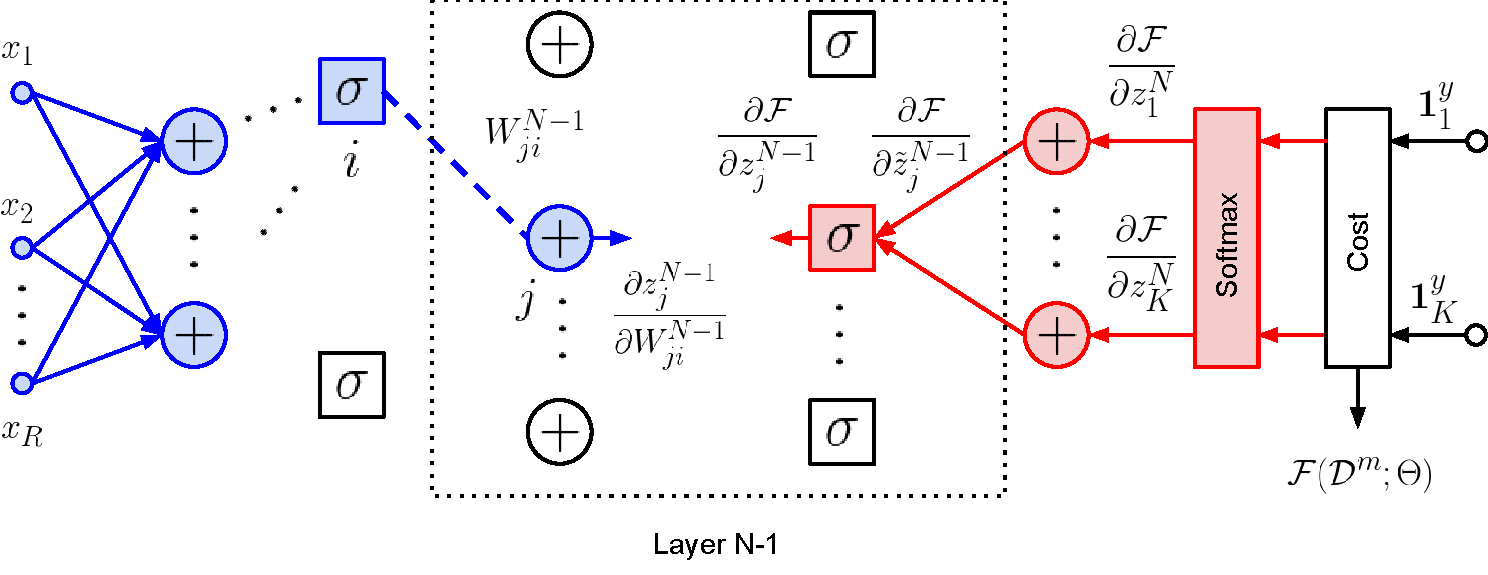
\includegraphics[scale=0.6]{figs/deep_learning/NN_backprop_colored.pdf}
\caption{Forward-pass (blue) and Backpropagation (red) calculations to estimate the gradient of weight $W_{ji}$ at layer $N-1$ of a MLP.}
\label{fig:NN_color}
\end{figure}

In a generic MLP we would like to compute the values of all parameters $\Theta=\{\mathbf{W}^1, \mathbf{b}^1, \cdots \mathbf{W}^N, \mathbf{b}^N\}$. As explained previously, we will thus need to compute the backpropagated error at each node $\partial \mathcal{F}(\mathcal{D}^m;\Theta)/\partial z_k^n$, and the corresponding derivative for the forward-pass $\partial z_k^n/\partial W_{ik}$, for $n = 1 \cdots N$. Fortunately, it is easy to spot a recursion that will allow us to compute these values for each node, given all its child nodes. To spot it, we can start trying to compute the gradients one layer before the output layer (see Fig.~\ref{fig:NN_color}), i.e. layer $N-1$. We start by splitting at $N-1$
%
\begin{align}
\frac{\partial \mathcal{F}(\mathcal{D}^m;\Theta)}{\partial W_{ji}} = \sum_{j'=1}^{J} {\color{red} \frac{\partial \mathcal{F}(\mathcal{D}^m;\Theta)}{\partial z_{j'}^{N-1}}} {\color{blue} \frac{\partial z_{j'}^{N-1}}{\partial W_{ji}}} = {\color{red} \frac{\partial \mathcal{F}(\mathcal{D}^m;\Theta)}{\partial z_{j}^{N-1}}} {\color{blue} \frac{\partial z_{j}^{N-1}}{\partial W_{ji}}}
\label{eq:BPderivation1}
\end{align}
%
where, as in the case of the log-linear model, we have used the fact that only $z_j$ depends on $W_{ji}$. We now advance forward from $z^N_j$ and apply the non-linearity to obtain $\tilde{z}^N_j$. As long as the non-linearity is a one-to-one operation (and this is often the case in neural-networks), we will also get rid of the summation leading to
%
\begin{align}
\frac{\partial \mathcal{F}(\mathcal{D}^m;\Theta)}{\partial W_{ji}} = \bigg(\sum_{j'=1}^{J} \frac{\partial \mathcal{F}(\mathcal{D}^m;\Theta)}{\partial \tilde{z}_{j'}^{N-1}} \frac{\partial \tilde{z}_{j'}^{N-1}}{\partial z_{j}^{N-1}}\bigg) \frac{\partial z_{j}^{N-1}}{\partial W_{ji}}= \frac{\partial \mathcal{F}(\mathcal{D}^m;\Theta)}{\partial \tilde{z}_{j}^{N-1}}\frac{\partial \tilde{z}_{j}^{N-1}}{\partial z_{j}^{N-1}}\frac{\partial z_{j}^{N-1}}{\partial W_{ji}}.
\label{eq:BPderivation2}
\end{align}
%
We will not be so lucky in the next application of the chain rule. Looking at Fig.~\ref{fig:NN_color}, it is clear that the derivatives at each node in layer $N-1$ will depend on all values of layer $N$. We thus have
%
\begin{align}
\frac{\partial \mathcal{F}(\mathcal{D}^m;\Theta)}{\partial W_{ji}} = \bigg(\sum_{k'=1}^{K} \frac{\partial \mathcal{F}(\mathcal{D}^m;\Theta)}{\partial z_{k'}^{N}} \frac{\partial z_{k'}^{N}}{\partial \tilde{z}_{j}^{N-1}}\bigg)\frac{\partial \tilde{z}_{j}^{N-1}}{\partial z_{j}^{N-1}}\frac{\partial z_{j}^{N-1}}{\partial W_{ji}}.
\label{eq:BPderivation3}
\end{align}
%
Now, comparing Eq.~\ref{eq:BPderivation1} with Eq.~\ref{eq:BPderivation3} it is easy to see that, if we denote the derivative of the cost (or error) with respect to the $N$ linear layer of the graph as
%
\begin{align}
e^{N-1} = \frac{\partial \mathcal{F}(\mathcal{D}^m;\Theta)}{\partial z_{k}^{N-1}} ,
\label{eq:BPderivation4}
\end{align}
%
\noindent then we can relate this to the cost derivative with respect to the preceding layer with
%
\begin{align}
e^{N-1} = \bigg(\sum_{k'=1}^{K} e^N \frac{\partial z_{k'}^{N}}{\partial \tilde{z}_{k'}^{N-1}}\bigg)\frac{\partial \tilde{z}_{k'}^{N-1}}{\partial z_{k'}^{N-1}} = \bigg(\sum_{k'=1}^{K} e^N_k W^N_{kj}\bigg)\cdot\tilde{z}_{k'}^{N-1}\cdot(1-\tilde{z}_{k'}^{N-1}),
\label{eq:chainRulRecursion}
\end{align}
%
where we have used the fact that for sigmoid non-linearities 
%
\begin{equation}
\frac{\partial \tilde{z}_{k}}{\partial z_{k}} = \tilde{z}_{k}\cdot (1-\tilde{z}_{k}).
\end{equation}

This formula can also be interpreted as traversing the graph in Fig.~\ref{fig:FF} backwards, multiplying at each node the backpropagated error by the derivative of its inputs and summing the errors propagated from different nodes. A more formal expression of the algorithm can be found in Algorithm~\ref{algo:backprop}.

\begin{algorithm}[th!]

   \caption{Mini-batch SGD with Back-Propagation}

\begin{algorithmic}[1]
\label{algo:backprop}

   \STATE {\bfseries input:} 
   %Data $\mathcal{D}$, Feed-forward of $N$ layers, with parameters $\Theta=\{\mathbf{W}^1, \mathbf{b}^1, \cdots \mathbf{W}^N, \mathbf{b}^N\}$, number of rounds $T$, $B$ mini-batches of size $M$, learning rate $\eta$
Data $\mathcal{D}=\{\mathcal{D}_1,\mathcal{D}_2,...,\mathcal{D}_B\}$ split into $B$ mini-batches of size $M'$%(in each data mini-batch $\mathcal{D}_b$ the example indicies $m$ range from 1 to $M'$)
, MLP of $N$ layers, with parameters $\Theta=\{\mathbf{W}^1, \mathbf{b}^1, \cdots \mathbf{W}^N, \mathbf{b}^N\}$, number of rounds $T$, learning rate $\eta$

   \STATE initialize parameters $\Theta$ randomly 

	\FOR{$t=1$ {\bfseries to} $T$}
	\FOR{$b=1$ {\bfseries to} $B$}

	\vspace{0.3cm}
	\FOR{$m=1$ {\bfseries to} $M'$}
	\STATE Compute the {forward pass} for each of the $M'$ examples in batch $b$; 
	 keep not only $p(y^m|\mathbf{x}^m) \equiv \tilde{\mathbf{z}}^{m,N}$ but also all the intermediate non-linear outputs $\tilde{\mathbf{z}}^{m,1} \cdots \tilde{\mathbf{z}}^{m,N}$.
	\ENDFOR	
	\vspace{0.3cm}
    %\STATE \textbf{Backpropagate} $\nabla_{\mathbf{z}^{m,n}}\mathcal{F}(\mathcal{D}_b;\Theta)$ 
	\FOR{$n=N$ {\bfseries to} $1$}
        \IF{n==N} 
		\FOR{$m=1$ {\bfseries to} $M'$}
        \STATE {Initialize the error at last layer, for each example $m$. For the softmax with CE cost this is given by:
        $$\mathbf{e}^{m,N} = \Big(\mathrm{\mathbf{1}}_{k(m)} - \tilde{\mathbf{z}}^{m,N} \Big).$$}
		\ENDFOR	
        \ELSE
   		\FOR{$m=1$ {\bfseries to} $M'$}
		\STATE {Backpropagate} the error through the linear layer, for each example $m$:  
        $$\mathbf{e}^{m,n} = \Big((\mathbf{W}^{n+1})^T \mathbf{e}^{m,n+1}\Big)$$ 
        
		\STATE {Backpropagate} the error through the non-linearity, for the sigmoid this is:  
        $$\mathbf{e}^{m,n} = \mathbf{e}^{m,n+1} \odot \tilde{\mathbf{z}}^{m,n} \odot (\mathbf{\mathrm{1}}-\tilde{\mathbf{z}}^{m,n}),$$
        where $\odot$ is the element-wise product and the $\mathbf{\mathrm{1}}$ is replicated to match the size of $\tilde{\mathbf{z}}^n$.


		\ENDFOR	
        \ENDIF 

		\vspace{0.3cm}
        \STATE {Compute the gradients} using the backpropagated errors and the inputs from the forward pass

        $$\nabla_{\mathbf{W}^n}\mathcal{F}(\mathcal{D_b};\Theta)  = -\frac{1}{M'} \sum_{m=1}^{M'} \mathbf{e}^{m,n} \cdot \left(\tilde{\mathbf{z}}^{m,n-1}\right)^T,$$ 
        $$\nabla_{\mathbf{b}^n}\mathcal{F}(\mathcal{D_b};\Theta)  = - \frac{1}{M'} \sum_{m=1}^{M'} \mathbf{e}^{m,n}.$$  

		\vspace{0.3cm}
        \STATE Update the parameters 
            $$\mathbf{W}^n \leftarrow \mathbf{W}^n - \eta \nabla_\mathbf{W^n}\mathcal{F},$$ 
            $$\mathbf{b}^n \leftarrow \mathbf{b}^n - \eta \nabla_\mathbf{b^n}\mathcal{F}.$$ 

	\ENDFOR

	\ENDFOR
	\ENDFOR
\end{algorithmic}
\end{algorithm}

\clearpage

\begin{exercise}
Start by loading Amazon sentiment corpus used in day \ref{day:classification}

\begin{python}
import numpy as np
import lxmls.readers.sentiment_reader as srs
scr = srs.SentimentCorpus("books")
train_x = scr.train_X.T
train_y = scr.train_y[:, 0]
test_x = scr.test_X.T
test_y = scr.test_y[:, 0]
\end{python}

Go to lxmls/deep\_learning/mlp.py:class NumpyMLP:def grads() and complete the
code of the NumpyMLP class with the Backpropagation recursion that we just saw.
Once you are done. Try different network geometries by increasing the number of
layers and layer sizes e.g.
\begin{python}
# Neural network modules
import lxmls.deep_learning.mlp as dl
import lxmls.deep_learning.sgd as sgd
# Model parameters
geometry = [train_x.shape[0], 20, 2]
actvfunc = ['sigmoid', 'softmax'] 
# Instantiate model
mlp      = dl.NumpyMLP(geometry, actvfunc) 
\end{python}
You can test the different hyperparameters 
\begin{python}
# Model parameters
n_iter = 5
bsize  = 5
lrate  = 0.01
# Train
sgd.SGD_train(mlp, n_iter, bsize=bsize, lrate=lrate, train_set=(train_x, train_y))
acc_train = sgd.class_acc(mlp.forward(train_x), train_y)[0]
acc_test  = sgd.class_acc(mlp.forward(test_x), test_y)[0]
print "MLP (%s) Amazon Sentiment Accuracy train: %f test: %f" % (geometry, acc_train,acc_test)
\end{python}
\end{exercise}

\subsection{Some final reflections on Backpropagation}

If you are new to the neural network topic, this is about the most important
piece of theory you should learn about deep learning. Here are some reflections
that you should keep in mind.

\begin{itemize}
\item Thanks to the multi-layer structure and the chain rule, Backpropagation allows models that compose linear and non-linear functions with any depth (in principle\footnotemark). 

\item The formulas are also valid for other cost functions and output layer non-linearities with minor modifications. It is only necessary to compute the equivalent of Eq.~\ref{eq:patialSoftmax}. 

\item The formulas are also valid for hidden non-linearities other than the sigmoid. Element-wise non-linear transformations still allow the simplification in Eq.~\ref{eq:chainRulRecursion}. With little effort it is also possible to deal with other cases.

\item However, there is an important limitation: unlike the log-linear models, the optimization problem is \textit{non convex}. This removes some formal guarantees, most importantly we can get trapped in local minima during training.
\end{itemize}

\footnotetext{Not exactly, since it is possible to run into numerical problems.}

% THIS WILL BE COMMENTED UNTIL THE FINAL UPDATE
%
%\subsection{A Note on Pre-Trainining}
%
%If you already have some experience with neural networks you might have
%realised that all what we show here is classic MLP theory, which is 30-40 years
%old. Indeed, it could be argued that, at the core, many modern deep learning
%applications are just classical neural networks theory with more data and more
%computing power. One of the novelties that came along the deep learning wave of
%research is pre-training with the Restricted Boltzmann Machine (RBM) paradigm.
%The cost function for a MLP of many layers becomes too complex and, as
%mentioned before, local minima and non-convexity make training of deep MLPs
%problematic. 
%
%The RBM paradigm allows to pre-train a MLP in \textit{unsupervised} fashion
%i.e. with out reference labels $\mathbf{y}^m$, which has been shown to improve
%posterior training. However, current state of the art systems do not always use
%RBM pre-training, resort to simpler types of smart-initializations or use none.
%Fort his reason, we will only see pre-training as an advance topic.  

%%%%%%%%%%%%%%%%%%%%%%%%%%%%%%%%%%%%%%%%%%%%%%%%%%%%%
\section{Deriving gradients and GPU code with Theano}
%%%%%%%%%%%%%%%%%%%%%%%%%%%%%%%%%%%%%%%%%%%%%%%%%%%%%

\subsection{An Introduction to Theano}

As you may have observed, the speed of SGD training for MLPs slows down
considerably when we increase the number of layers. One reason for this is that
the code that we use here is not very optimized. It is thought for you to
learn the basic principles. Even if the code was more optimized, it would still be
very slow for reasonable network sizes. The cost of computing each
linear layer is proportional to the dimensionality of the previous and current
layers, which in most cases will be rather large. 

For this reason most deep learning applications use Graphics Processing Units
(GPU) in their computations. This specialized hardware is normally used to
accelerate computer graphics, but can also be used for general computation
intensive tasks. However, we need to deal with specific interfaces and
operations in order to use a GPU. This is where Theano comes in. Theano is a
multidimensional symbolic expression python module with focus on neural
networks. It will provide us with the following nice features:

\begin{itemize}
\item Symbolic expressions: Express the operations of the MLP (forward pass, cost) symbolically, as mathematical operations rather than explicit code 
\item Symbolic Differentiation: As a consequence of the previous feature, we can compute gradients of arbitrary mathematical functions automatically.   
\item GPU integration: The code will be ready to work on a GPU, provided that you have one and it is active within Theano. It will also be faster on normal CPUs since the symbolic operations are compiled to C code. 
\item Theano is focused on Deep Learning, with an active community and several tutorials easily available.  
\end{itemize}

\noindent However, this does not come at a free price. There are a number of limitations

\begin{itemize}
\item Symbolic algebra is more difficult to debug, as we can not easily step in at each operation. 
\item Working with CPU and GPU code implies that we have to be more careful about the types of the variables.
\item Theano tends to output long error messages. However, once you get used to it, error messages accurately point the source of the problem. 
\item Handling recurrent neural networks is much simpler than in Numpy but it still implies working with complicated constructs that are complicated to debug. 
\end{itemize}

\begin{exercise}
\label{exerciseTheano1}
Get in contact with Theano. Learn the difference between a symbolic
representation and a function. Start by implementing the first layer of our
previous MLP in Numpy 
\begin{python}
# Numpy code
x        = test_x             # Test set 
W1, b1   = mlp.params[:2]     # Weights and bias of fist layer 
z1       = np.dot(W1, x) + b1 # Linear transformation
tilde_z1 = 1/(1+np.exp(-z1))  # Non-linear transformation  
\end{python}
Now we will implement this in Theano.  We start by creating the variables over
which we will produce the operations. For example the symbolic input is defined
as
\begin{python}
# Theano code. 
# NOTE: We use undescore to denote symbolic equivalents to Numpy variables. 
# This is no Python convention!.
import theano
import theano.tensor as T
_x = T.matrix('x')
\end{python}

Note that this variable does not have any particular value, nor a space
reserved in memory for it. It contains just a symbolic definition of what the
variable can contain. The particular values will be given when we use it to
compile a function. 

We could actually use the same definition format to define the weights and give
their particular values as inputs to the compiled function. However, since we
will be using a more complicated format in later exercises, we will use it here
as well. The \textit{shared} class allows to define variables that are shared
across functions. They are also given a concrete value so that we do not need
to give it for each function call. This format is therefore ideal for the
weights of our network.
\begin{python}
_W1 = theano.shared(value=W1, name='W1', borrow=True) 
_b1 = theano.shared(value=b1, name='b1', borrow=True, broadcastable=(False, True)) 
\end{python}

\textbf{Important:} One of the main differences between Numpy and theano data
is broadcast. In Numpy if we sum an array with shape (N, M) to one with shape
(1, M), the second array will be copied N times to form a (N, M) matrix. This
is known as broadcasting. In Theano this is not automatic. You need to specify
broadcasting explicitly. This is important for example when using a bias, which
will be copied to match the number of examples in the batch. In other cases,
like when using variables for recurrent neural networks, broadcast has to be
set to False. Broadcast is one of the typical source of errors when you start
working with Theano. Keep this in mind.

Now lets describe the operations we want to do with the variables. Again only
symbolically. This is done by replacing our usual operations by Theano symbolic
ones when necessary e. g. the internal product dot() or the sigmoid. Some
operations like e.g. $+$ are automatically recognized by Theano (operator
overloading). 
\begin{python}
_z1            = T.dot(_W1, _x) + _b1
_tilde_z1      = T.nnet.sigmoid(_z1)
# Keep in mind that naming variables is useful when debugging
_z1.name       = 'z1'
_tilde_z1.name = 'tilde_z1'
\end{python}
When debugging the code it is often useful to print the graph of computations.
\begin{python}
# Perceptron computation graph
theano.printing.debugprint(_tilde_z1)

sigmoid [@A] 'tilde_z1'
 |Elemwise{add,no_inplace} [@B] 'z1'
   |dot [@C] ''
   | |W1 [@D]
   | |x [@E]
   |b1 [@F]

\end{python}
It is important to keep in mind that, until this point, we do not have a
function we can use to produce any practical input. In order to obtain this we
have to compile this function by calling    
\begin{python}
layer1 = theano.function([_x], _tilde_z1)
\end{python}
Note the use of $[$ $]$ for the input variables, even if we just specify one
variable. We can now do a test to compare the Numpy and Theano implementations
and see that they give the same outputs.
\begin{python}
# Check Numpy and Theano match
assert np.allclose(tilde_z1, layer1(x.astype(theano.config.floatX))), \
    "Numpy and Theano Perceptrons are different"
\end{python}
\end{exercise}

One of the main sources of errors in Theano is the type of the arrays used. To
ensure compatibility with the GPU check every array that you are going to work
with and be sure it has the propper type To automatically switch between
float64 (CPU) and float32 (GPU) types Theano provides the floatX type. Keep in
mind not using these is the number one source of errors when you start with
Theano.
%
\begin{python}
train_x = train_x.astype(theano.config.floatX)
train_y = train_y.astype('int32')
\end{python}
%
\subsection{Symbolic Forward Pass}
In the previous section you have seen how to create symbolic Theano functions
with shared parameters. You have thus all you need to implement the whole
forward pass of a generic MLP in Theano.
\begin{exercise}
Complete the method \_forward() inside of the lxmls/deep\_learning/mlp.py:class
TheanoMLP. Note that this is called only once at the initialization of the
class. To debug your implementation put a breakpoint at the \_\_init\_\_
function call. Hint: Note that this is very similar to NumpyMLP.forward().
You just need to keep track of the symbolic variable representing the output of
the network after each layer is applied and compile the function at the end.
After you are finished instantiate a Theano class and check that Numpy and
Theano forward pass are the same. 

\begin{python}
mlp_a = dl.NumpyMLP(geometry, actvfunc)
mlp_b = dl.TheanoMLP(geometry, actvfunc)
\end{python}

To help debugging in Theano is sometimes useful to switch off the optimizer.
This helps Theano point out which part of the Python code generated the error
\begin{python}
theano.config.optimizer='None'
\end{python}
In general, the best way to debug Theano is to \textbf{compile often}. Try to
compile the intermediate variables and perform the algebraic operations in
Numpy. Once you are done, the following code should yield no error

\begin{python}
assert np.allclose(mlp_a.forward(test_x), mlp_b.forward(test_x)), \
    "ERROR: Numpy and Theano forward passes differ"
\end{python}
\end{exercise}

\subsection{Symbolic Differentiation}
In the previous section we compiled the forward pass of a MLP. In this section
we will do the same with the cost used for training. We will also derive the
gradients although this will be trivial once we have the cost function compiled.     
\begin{exercise}
We first see an example that does not use any of the code in TheanoMLP but
rather continues from what you wrote in Ex. \ref{exerciseTheano1}. In this exercise you
completed a sigmoid layer with Theano. To get some values for the weights we
used the first layer of the network you trained in \ref{exerciseTheano1}. Now we are going to use
the second layer as well. This is thus assuming that your network in \ref{exerciseTheano1} has
only two layers e.g. the recommended geometry (I, 20, 2). Make sure this is the
case before starting this exercise.  

\noindent For the sake of clarity, lets write here the part of Ex. \ref{exerciseTheano1} that we had completed
\begin{python}
# Get the values from our MLP 
W1, b1   = mlp.params[:2]     # Weights and bias of fist layer 
# First layer symbolic variables
_x  = T.matrix('x')
_W1 = theano.shared(value=W1, name='W1', borrow=True) 
_b1 = theano.shared(value=b1, name='b1', borrow=True, broadcastable=(False, True)) 
# First layer symbolic expressions
_z1       = T.dot(_W1, _x) + _b1
_tilde_z1 = T.nnet.sigmoid(_z1)
\end{python}
Now we just need to complete this with the second layer, using a softmax non-linearity
\begin{python}
W2, b2  = mlp.params[2:]     # Weights and bias of second (and last!) layer 
# Second layer symbolic variables
_W2 = theano.shared(value=W2, name='W2', borrow=True) 
_b2 = theano.shared(value=b2, name='b2', borrow=True, broadcastable=(False, True)) 
# Second layer symbolic expressions
_z2       = T.dot(_W2, _tilde_z1) + _b2
_tilde_z2 = T.nnet.softmax(_z2.T).T
\end{python}
With this, we could compile a function to obtain the output of the network
symb\_tilde\_z2 for a given input symb\_x. In this exercise we are however
interested in obtaining the misclassification cost. This is given in Eq:
\ref{eq:CostLogPos}. First we are going to need the symbolic variable for the
correct output
\begin{python}
_y = T.ivector('y')
\end{python}
The minus posterior probability of the class given the input is the same as
selecting the $k(m)$-th softmax output, were $k(m)$ is the index of the correct
class for $x^m$. If we want to do this for a vector $\mathbf{y}$ containing $M$
different examples, we can write this as
\begin{python}
_F = -T.mean(T.log(_tilde_z2[_y, T.arange(_y.shape[0])]))
\end{python}
Now obtaining a function that computes the gradient could not be easier.
\begin{python}
_nabla_F = T.grad(_F, _W1) 
nabla_F  = theano.function([_x, _y], _nabla_F) 
\end{python}
To finish this exercise have a look at the TheanoMLP class. As you may realise
it just implements what is shown above for the generic case of $N$ layers. 
\end{exercise}


\subsection{Symbolic mini-batch update}

One important aspect to take into account is that to obtain a good speed up,
the batch update operation must be carried out inside of Theano. To do this
we may use the updates argument of theano.function

\begin{exercise}
Define the updates list. This is a list where each element is a tuple of a 
parameter and the update rule to be applied that parameter. In this case we 
are defining the SGD update rule, but take into account that using more complex
update rules like e.g. momentum or adam implies just replacing the last line
of the following snippet.
\begin{python}
mlp_c   = dl.TheanoMLP(geometry, actvfunc)
_x      = T.matrix('x')
_y      = T.ivector('y')
_F      = mlp_c._cost(_x, _y)
# SGD update rule
updates = [(par, par - lrate*T.grad(_F, par)) for par in mlp_c.params]
\end{python}

\noindent This will return the cost of each batch and update the MLP parameters
at the indent same time using updates
\begin{python}
batch_up = theano.function([_x, _y], _F, updates=updates)
n_batch  = int(np.ceil(float(train_x.shape[1])/bsize))
\end{python}
Once we have defined this, we can compare speed and accuracy of the Numpy and
simple gradient versions using

\begin{python}
import time
# Model
geometry = [train_x.shape[0], 20, 2]
actvfunc = ['sigmoid', 'softmax'] 

# Numpy MLP
mlp_a     = dl.NumpyMLP(geometry, actvfunc)
init_t    = time.clock()
sgd.SGD_train(mlp_a, n_iter, bsize=bsize, lrate=lrate, train_set=(train_x, train_y))
print "\nNumpy version took %2.2f sec" % (time.clock() - init_t)
acc_train = sgd.class_acc(mlp_a.forward(train_x), train_y)[0]
acc_test  = sgd.class_acc(mlp_a.forward(test_x), test_y)[0]
print "Amazon Sentiment Accuracy train: %f test: %f\n" % (acc_train, acc_test)

# Theano grads 
mlp_b  = dl.TheanoMLP(geometry, actvfunc)
init_t = time.clock()
sgd.SGD_train(mlp_b, n_iter, bsize=bsize, lrate=lrate, train_set=(train_x, train_y))
print "\nCompiled gradient version took %2.2f sec" % (time.clock() - init_t)
acc_train = sgd.class_acc(mlp_b.forward(train_x), train_y)[0]
acc_test  = sgd.class_acc(mlp_b.forward(test_x), test_y)[0]
print "Amazon Sentiment Accuracy train: %f test: %f\n" % (acc_train, acc_test)

# Theano batch update
init_t = time.clock()
sgd.SGD_train(mlp_c, n_iter, batch_up=batch_up, n_batch=n_batch, bsize=bsize, 
              train_set=(train_x, train_y))
print "\nTheano compiled batch update version took %2.2f" % (time.clock() - init_t)
acc_train = sgd.class_acc(mlp_c.forward(train_x), train_y)[0]
acc_test  = sgd.class_acc(mlp_c.forward(test_x), test_y)[0]
print "Amazon Sentiment Accuracy train: %f test: %f\n"%(acc_train,acc_test)
\end{python}
As you may observe, just computing the gradients with Theano may not lead to
a decrease, but rather an increase in computing time. To maximally exploit
the power of Theano, it is necessary to bundle both computations and data 
together using approaches like the compiled batch update.
\end{exercise}


\chapter{\label{day:seq_disc}Learning Structured Predictors}
In this class, we will continue to focus on sequence classification,
but instead of following a \emph{generative} approach (like in the previous
chapter) we move towards \emph{discriminative} approaches. Recall that the difference between these approaches is that generative approaches attempt to model the probability distribution of the data, $P(X,Y)$, whereas discriminative ones only model the conditional probability of the sequence, given the observed data, $P(Y|X)$.



\section*{Today's Assignment}

The assignment of today's class is to implement the structured version of the perceptron algorithm.

\section{Classification vs Sequential Classification}


Table \ref{disc_seq_summary} shows how the models for classification 
have counterparts in \emph{sequential} classification. In fact, in
the last chapter we discussed the Hidden Markov model, which can be seen as a
generalization of the Na\"{i}ve Bayes model for sequences. 
In this chapter, we will see a generalization of the
Perceptron algorithm for sequence problems (yielding the Structured
Perceptron, \citealt{collins2002discriminative}) and a generalization of
Maximum Entropy model for sequences (yielding Conditional Random Fields, \citealt{lafferty2001conditional}). 
Note that both these generalizations are  not specific for sequences
and can be applied to a wide range of models (we will see in tomorrow's
lecture how these methods can be applied to parsing).
Although we will not cover all the methods described in
Chapter \ref{day:classification}, bear in mind that all of those have a structured counterpart. 
It should be intuitive after this lecture how those methods could be
extended to structured problems, given the perceptron example.
%Before we explain the particular methods, the next section will talk a bit about feature representation for sequences. 

\begin{table}[h!]
\centering
\begin{tabular}{|l|l|}
\hline
\multicolumn{1}{|c|}{\textbf{Classification}} & \multicolumn{1}{|c|}{\textbf{Sequences}} \\
\hline
\multicolumn{2}{|c|}{\emph{Generative}}\\
\hline
Na\"{i}ve Bayes~(Sec.~\ref{s::naiveBayes}) & Hidden Markov Models~(Sec.~\ref{hmm}) \\
\hline
\multicolumn{2}{|c|}{\emph{Discriminative}}\\
\hline
Perceptron~(Sec.~\ref{s:perceptron}) & Structured Perceptron~(Sec.~\ref{s:spercetron})\\
\hline
Maximum Entropy~(Sec.~\ref{s:me}) & Conditional Random Fields~(Sec.~\ref{s:crf})\\
\hline
\end{tabular}
\caption{\label{disc_seq_summary}Summary of the methods used for classification and sequential classification covered in this guide.}
\end{table}


Throughout this chapter, we will be searching for the solution of 
\begin{equation}
\argmax_{y \in \statevocab^N} P(Y=y | X=x) = \argmax_{y \in \statevocab^N} \W \cdot  \F(x,y). \label{eq::struc_pred} 
\end{equation}
where $\W$ is a weight vector, and $\F(x,y)$ is a feature vector. We will see that this sort of linear models are more flexible than HMMs, in the sense that they may incorporate 
more general features while being able to reuse the same decoders (based on the Viterbi and forward-backward algorithms). In fact, \emph{the exercises in this lab will not touch the decoders that 
have been developed in the previous lab}. 
Only the training algorithms and the function that 
compute the scores will change.

As in the previous section, $y = y_1\ldots y_N$ is a sequence so the maximization
is over an exponential number of objects, making it intractable for brute force methods. Again
we will make an assumption analogous to the ``first order Markov independence property,'' so that the
features may decompose as a sum over nodes and edges in a trellis. 
This is done by assuming that expression~\ref{eq::struc_pred} can be written as:
\begin{equation}
\argmax_{y \in \statevocab^N} 
\sum_{i=1}^N \underbrace{\W \cdot \F_{\mathrm{emiss}}(i,x,y_i)}_{\mathrm{score}_{\mathrm{emiss}}}  + 
\underbrace{\W \cdot \F_{\mathrm{init}}(x,y_1)}_{\mathrm{score}_{\mathrm{init}}}  + 
\sum_{i=1}^{N-1} \underbrace{\W \cdot \F_{\mathrm{trans}}(i,x,y_i,y_{i+1})}_{\mathrm{score}_{\mathrm{trans}}}+ 
\underbrace{\W \cdot \F_{\mathrm{final}}(x,y_N)}_{\mathrm{score}_{\mathrm{final}}}
\label{eq::struc_pred_decompose}
\end{equation}
In other words, the scores ${\mathrm{score}_{\mathrm{emiss}}}$, 
${\mathrm{score}_{\mathrm{init}}}$, ${\mathrm{score}_{\mathrm{trans}}}$
and ${\mathrm{score}_{\mathrm{final}}}$ are now computed as inner products 
between weight vectors and feature vectors rather than log-probabilities.
The feature vectors depend locally on the output variable 
(\emph{i.e.}, they only look at a single $y_i$ or a pair $y_i,y_{i+1}$);
however they may depend globally on the observed input $x=x_{1},\ldots,x_{N}$.


\section{\label{seq::features} Features}

In this section we will define two simple feature sets.\footnote{Although not required, all the features we will use are binary features, indicating whether a given condition 
is satisfied or not.} The first feature set
will only use identity features, and will mimic the features used by
the HMM model from the previous section. This will allow us to directly
compare the performance of a generative vs a discriminative
approach. %\begin{example}
%Simple ID Feature set containing the same features as an HMM model.
%\begin{python}
%0 Ms./NOUN NF: id:Ms.::NOUN init_tag:NOUN 
%1 Haag/NOUN NF: id:Haag::NOUN EF: prev_tag:NOUN::NOUN 
%2 plays/VERB NF: id:plays::VERB EF: prev_tag:NOUN::VERB 
%3 Elianti/NOUN NF: id:Elianti::NOUN EF: prev_tag:VERB::NOUN 
%4 ./. NF: id:.::. EF: last_prev_tag:NOUN::. 
%\end{python}
%\end{example}
Table~\ref{id-features} depicts the features that are implicit in the HMM, which was the subject of 
the previous chapter. These features are indicators of initial, transition, final, and emission events.

\begin{table}[h!]
\begin{center}
\begin{tabular}{|l|l|}
\hline
Condition & Name\\
\hline
$y_i = c_k \text{  } \& \text{  } i =0 $& Initial Features \\
\hline
$y_i = c_k \text{  } \& \text{  } y_{i-1} = c_l$& Transition Features \\
\hline
$y_i = c_k \text{  } \& \text{  } i = N$& Final Features \\
\hline
$x_i = w_j \text{  } \& \text{  } y_i = c_k$ & Emission Features \\
\hline
\end{tabular}
\caption{\label{id-features} {\tt IDFeatures} feature set. This set
  replicates the features used by the HMM model.}
\end{center}
\end{table}
 
 
Note that the fact that we were using a generative model has forced us (in some sense) to 
make strong independence assumptions. 
However, since we now move to a discriminative approach, where we model $P(Y|X)$ rather than $P(X,Y)$, we are not tied anymore to 
some of these assumptions. In particular: 
\begin{itemize}
\item We may use ``overlapping'' features, \emph{e.g.}, features that fire simultaneously for many instances. 
For example, we can use a feature for a word, such as a feature which fires for the word "brilliantly", and another for prefixes and suffixes of that word, such as one which fires if the last two letters of the word are "ly".
This would lead to an awkward model if we wanted to insist on a generative approach. 
\item We may use features that depend arbitrarily on the \emph{entire input sequence} $x$. On the other hand, 
we still need to resort to ``local'' features with respect to the \emph{outputs} (\emph{e.g.} looking only at consecutive state pairs), 
otherwise decoding algorithms will become more expensive.  
\end{itemize}


This leads us to the second feature set, composed of features that are traditionally used in POS tagging with discriminative models. See Table~\ref{ex-features} for some examples.
Of course, we could have much more complex features, looking arbitrarily to 
the input sequence. We are not going to have them in this
exercise only for performance reasons (to have less features and smaller caches). State-of-the-art sequence classifiers can easily reach over one million features!

\begin{table}[h!]
\begin{center}
\begin{tabular}{|l|l|}
\hline
Condition & Name\\
\hline
$y_i = c_k \text{  } \& \text{  } i =0 $& Initial Features \\
\hline
$y_i = c_k \text{  } \& \text{  } y_{i-1} = c_l$& Transition Features \\
\hline
$y_i = c_k \text{  } \& \text{  } i = N$& Final Features \\
\hline
$x_i = w_j \text{  } \& \text{  } y_i = c_k$& Basic Emission Features \\
$x_i = w_j \text{  } \& \text{ $w_j$ is uppercased} \text{  } \& \text{  } y_i = c_k$& Uppercase Features
\\
$x_i = w_j \text{  } \& \text{ $w_j$ contains digit} \text{  } \& \text{  } y_i = c_k$& Digit Features
\\
$x_i = w_j \text{  } \& \text{ $w_j$ contains hyphen} \text{  } \& \text{  } y_i = c_k$& Hyphen Features
\\
$x_i = w_j \text{  } \& \text{  } w_j[0..i] \forall i \in [1,2,3]
\text{  } \& \text{  } y_i = c_k$& Prefix Features \\
$x_i = w_j \text{  } \& \text{  } w_j[|w_j|-i..|w_j|] \forall i \in [1,2,3] \text{  } \& \text{  } y_i = c_k$& Suffix Features \\
\hline
\end{tabular}
\caption{\label{ex-features} {\tt Extended} feature set. Some features in this set could not be included in the HMM model. The features included in the bottom row are all considered emission features 
for the purpose of our implementation, since they all depend on $i$, $x$ and $y_i$.}
\end{center}
\end{table}



%\begin{example}
%
%\begin{python}
%0 Ms./NOUN NF: id:Ms.::NOUN uppercased::NOUN suffix:.::NOUN suffix:s.::NOUN prefix:M::NOUN prefix:Ms::NOUN init_tag:NOUN 
%1 Haag/NOUN NF: id:Haag::NOUN uppercased::NOUN suffix:g::NOUN suffix:ag::NOUN suffix:aag::NOUN prefix:H::NOUN prefix:Ha::NOUN prefix:Haa::NOUN rare::NOUN EF: prev_tag:NOUN::NOUN 
%2 plays/VERB NF: id:plays::VERB EF: prev_tag:NOUN::VERB 
%3 Elianti/NOUN NF: id:Elianti::NOUN uppercased::NOUN suffix:i::NOUN suffix:ti::NOUN suffix:nti::NOUN prefix:E::NOUN prefix:El::NOUN prefix:Eli::NOUN rare::NOUN EF: prev_tag:VERB::NOUN 
%4 ./. NF: id:.::. EF: last_prev_tag:NOUN::. 
%\end{python}
%\end{example}



Our features subdivide into two groups: 
$\F_{\mathrm{emiss}}$, $\F_{\mathrm{init}}$, 
and $\F_{\mathrm{final}}$ are all instances of 
\emph{node features}, 
depending only on a single position in the
state sequence (a node in the trellis); 
$\F_{\mathrm{trans}}$ 
are \emph{edge features},
depending on two consecutive positions in the state 
sequence (an edge in the trellis).
Similarly as in the previous chapter, we have the following scores (also called 
\emph{log-potentials} in the literature on CRFs and graphical models):
\begin{itemize}
\item \emph{Initial scores.}
These are scores for the initial state. 
They are given by 
\begin{equation}
{\mathrm{score}}_{\mathrm{init}}(x,y_1) = \W \cdot \F_{\mathrm{init}}(x,y_1).
\end{equation} 
\item \emph{Transition scores.}
These are scores for two consecutive states at a particular position. 
They are given by 
\begin{equation}
{\mathrm{score}}_{\mathrm{trans}}(i,x,y_i,y_{i+1}) = \W \cdot \F_{\mathrm{trans}}(i,x,y_{i},y_{i+1}).
\end{equation} 
\item \emph{Final scores.}
These are scores for the final state. 
They are given by 
\begin{equation}
{\mathrm{score}}_{\mathrm{final}}(x,y_N) = \W \cdot \F_{\mathrm{final}}(x,y_N).
\end{equation} 
\item \emph{Emission scores.}
These are scores for a state at a particular position. 
They are given by 
\begin{equation}\label{dis_node_potentials}
{\mathrm{score}}_{\mathrm{emiss}}(i,x,y_i) = \W \cdot \F_{\mathrm{emiss}}(i,x,y_i).
\end{equation} 
\end{itemize}
%which form a vector $\boldsymbol{f}_N(\sent,\hv_i)$, 
%and \emph{edge features}, which form a vector $\boldsymbol{f}_E(\sent,\hv_i,\hv_{i-1})$.% 
%\footnote{To make things simpler, we will assume later on that edge features do not depend on the input $\sent$---but they could, without 
%changing at all the decoding algorithm.} %
%These feature vectors will receive parameter vectors $\boldsymbol{\theta}_N$ and  $\boldsymbol{\theta}_E$. 
%Similarly as in the previous chapter, we consider:
%\begin{itemize}
%\item\emph{Node Potentials.} These are scores for a state at a particular position. 
% They are given by 
% \begin{equation}\label{dis_node_potentials}
% \psi_V(\sent,\hs_i) = \exp(\boldsymbol{\theta}_V \cdot \boldsymbol{f}_V(\sent,\hs_i)).
% \end{equation}
%\item\emph{Edge Potentials.} These are scores for the transitions. They are given by 
% \begin{equation}\label{dis_edge_potentials}
%\psi_E(\sent,\hs_i,\hs_{i-1}) = \exp(\boldsymbol{\theta}_E \cdot \boldsymbol{f}_E(\sent,\hs_i,\hs_{i-1})). 
% \end{equation}
%\end{itemize}
%
%Let $\boldsymbol{\theta} = (\boldsymbol{\theta}_N, \boldsymbol{\theta}_E)$. 

\section{Discriminative Sequential Classifiers}

Given a weight vector $\W$, the conditional probability $P_{\W}(Y=y|X=x)$ is then defined as follows: 
\begin{eqnarray}
\lefteqn{P_{\W}(Y=y|X=x) =}\nonumber\\
&&
\!\!\!\!\!\!\!\!\frac{1}{Z({\W},x)}\exp\left(\W \cdot \F_{\mathrm{init}}(x,y_1) + 
\sum_{i=1}^{N-1} \W \cdot \F_{\mathrm{trans}}(i,x,y_i,y_{i+1})
+
\W \cdot \F_{\mathrm{final}}(x,y_N)
+
\sum_{i=1}^{N} \W \cdot \F_{\mathrm{emiss}}(i,x,y_i)
\right) \label{eq:disc_formula}
%&=& \frac{1}{Z(\boldsymbol{\theta},x)} \prod_i\psi_V(\sent_i,\hs_i) \psi_E(\sent_i,\hs_i,\hs_{i-1}),
\end{eqnarray}
where the normalizing factor $Z(\W,x)$ is called the \emph{partition function}:
\begin{eqnarray}
\lefteqn{Z(\W,x) =}\nonumber\\ 
&& 
\sum_{y\in \statevocab^N} \exp\left(\W \cdot \F_{\mathrm{init}}(x,y_1) + 
\sum_{i=1}^{N-1} \W \cdot \F_{\mathrm{trans}}(i,x,y_i,y_{i+1})
+
\W \cdot \F_{\mathrm{final}}(x,y_N)
+
\sum_{i=1}^{N} \W \cdot \F_{\mathrm{emiss}}(i,x,y_i)
\right).
\end{eqnarray}


\subsection{Training}

For training, 
the important problem is that of obtaining the weight vector $\W$ that lead to an accurate 
classifier. 
We will discuss two possible strategies:
\begin{enumerate}
\item Maximizing conditional log-likelihood from a set of labeled data $\{(x^m,y^m)\}_{m=1}^M$, yielding \textbf{conditional random fields}. This corresponds to the following optimization problem:
\begin{equation}
\widehat{\W} = \argmax_{\W} \sum_{m=1}^M \log P_{\W}(Y=y^m | X=x^m).
\end{equation}
To avoid overfitting, it is common to regularize with the Euclidean norm function, 
which is equivalent to considering a zero-mean Gaussian prior on the weight vector.
The problem becomes:
\begin{equation}
\widehat{\W} = \argmax_{\W} \sum_{m=1}^M \log P_{\W}(Y=y^m | X=x^m) - \frac{\lambda}{2} \|\W\|^2.
\end{equation}
This is precisely the structured variant of the maximum entropy 
method discussed in Chapter 1.
Unlike HMMs, this problem does not have a closed form solution 
and has to be solved with numerical optimization. 
\item Alternatively, running the \textbf{structured perceptron} algorithm 
to obtain a weight vector $\W$ that accurately
classifies the training data. 
We will see that this simple strategy achieves results which are competitive 
with conditional log-likelihood maximization.
\end{enumerate}

\subsection{Decoding}

For decoding,  
there are three important problems that need to be solved: 
\begin{enumerate}
\item Given $X=x$, compute the most likely output sequence $\widehat{y}$ (the one which maximizes $P_{\W}(Y=y|X=x)$). 
\item Compute the posterior marginals $P_{\W}(Y_i=y_i|X=x)$ at each position $i$.
\item Evaluate the partition function $Z(\W,x)$. 
\end{enumerate}
Interestingly, all these problems can be solved by using the very same
algorithms that were 
already implemented for HMMs: the Viterbi algorithm (for 1) and the forward-backward algorithm (for 2--3). All that changes is the way the scores are computed. 

\section{\label{s:crf}Conditional Random Fields}

Conditional Random Fields (CRF)~\citep{lafferty2001conditional} can be seen
as an extension of the Maximum Entropy (ME) models  to structured problems.%
\footnote{An earlier, less successful, attempt to perform such an extension was via Maximum Entropy Markov
models (MEMM)~\citep{mccallum2000maximum}. There each factor (a node or edge) 
is a \emph{locally} normalized maximum entropy model. A shortcoming of MEMMs is its 
so-called \emph{labeling bias} \citep{Bottou1991}, which makes them biased towards states
with few successor states (see \cite{lafferty2001conditional} for more information).}
They are \emph{globally} normalized models: the probability of a given
sentence is given by Equation \ref{eq:disc_formula}. 
There are only two differences with respect to the standard ME model 
described a couple of days ago for multi-class classification: 
\begin{itemize}
\item Instead of computing the posterior marginals $P(Y=y|X=x)$ for all possible configurations
of the output variables (which are exponentially many), it 
assumes the model decompose into ``parts'' (in this case, nodes and edges), and it computes only 
the posterior marginals for those parts, 
  $P(Y_i=y_i | X=x)$ and  $P(Y_i=y_i, Y_{i+1}=y_{i+1}| X=x)$. 
Crucially, \textbf{we can compute these quantities by using the very same forward-backward algorithm that we have described for HMMs}.
\item Instead of updating the features for all possible outputs $y' \in \Lambda^N$, 
we again exploit the decomposition into parts above and update only 
``local features'' at the nodes and edges.
\end{itemize}

Algorithm
\ref{alg:crf_online} shows the pseudo code to optimize a CRF with 
the stochastic gradient descent (SGD) algorithm  
(our toolkit also includes an implementation of a quasi-Newton method, L-BFGS, 
which converges faster, but for the purpose of this exercise, we will 
stick with SGD). 

\begin{algorithm}[h!]
   \caption{SGD for Conditional Random Fields \label{alg:crf_online}}
\begin{algorithmic}[1]
   \STATE {\bfseries input:} $\mathcal{D}$, $\lambda$, number of rounds $T$,
   learning rate sequence $(\eta_t)_{t = 1,\ldots,T}$
   \STATE initialize $\W^1 = \mathbf{0}$
	\FOR{$t=1$ {\bfseries to} $T$}
	\STATE choose $m=m(t)$ randomly
	\STATE take training pair $(x^m, y^m)$ and compute the probability 
	$P_{\W}(Y=y^m|X=x^m)$ using the current model ${\W}$ and Eq.~\ref{eq:disc_formula}.
	\STATE for every $i$, $y_i'$, and $y_{i+1}'$, 
	compute marginal probabilities $P(Y_i=y_i' | X=x)$ and  $P(Y_i=y_i', Y_{i+1}=y_{i+1}'| X=x^m)$ 
	using the current model $\W$, for each node and edge, 
        through the forward-backward algorithm.
	\STATE compute the feature vector expectation:  
	\begin{eqnarray}
	E_{\W^t}[\F(x^m,Y)] &=& \sum_{y_1} P(y_1|x^m)\F_{\mathrm{init}}(x^m,y_1) +\nonumber\\
	&& \sum_{i=1}^{N-1}\sum_{y_i,y_{i+1}} P(y_i,y_{i+1}|x^m)\F_{\mathrm{trans}}(i,x^m,y_i,y_{i+1}) +\nonumber\\
	&& \sum_{y_N} P(y_N|x^m)\F_{\mathrm{final}}(x^m,y_N) +\nonumber\\
	&& \sum_{i=1}^{N}\sum_{y_i} P(y_i|x^m)\F_{\mathrm{emiss}}(i,x^m,y_i).
	\end{eqnarray}
	\STATE update the model: 
	$$\W^{t+1} \leftarrow (1-\lambda \eta_t) \boldsymbol{\W}^{t} + \eta_t \left( \F(x^m,y^m) 
	- E_{\W^t}[\F(x^m,Y)]\right)$$
	\ENDFOR
   \STATE \textbf{output:} $\widehat{\W} \leftarrow \W^{T+1}$
\end{algorithmic}
\end{algorithm}


\begin{exercise}\label{exer:crf1}
In this exercise you will train a CRF
using different feature sets for \pos\ Tagging. Start with the code below, which uses the ID feature set from table \ref{id-features}.
\begin{python}
import lxmls.sequences.crf_online as crfo
import lxmls.sequences.structured_perceptron as spc
import lxmls.readers.pos_corpus as pcc
import lxmls.sequences.id_feature as idfc
import lxmls.sequences.extended_feature as exfc

print("CRF Exercise")

corpus = pcc.PostagCorpus()
train_seq = corpus.read_sequence_list_conll("data/train-02-21.conll",max_sent_len=10,max_nr_sent=1000)
test_seq = corpus.read_sequence_list_conll("data/test-23.conll",max_sent_len=10,max_nr_sent=1000)
dev_seq = corpus.read_sequence_list_conll("data/dev-22.conll",max_sent_len=10,max_nr_sent=1000)
feature_mapper = idfc.IDFeatures(train_seq)
feature_mapper.build_features()

crf_online = crfo.CRFOnline(corpus.word_dict, corpus.tag_dict, feature_mapper)
crf_online.num_epochs = 20
crf_online.train_supervised(train_seq)

Epoch: 0 Objective value: -5.779018
Epoch: 1 Objective value: -3.192724
Epoch: 2 Objective value: -2.717537
Epoch: 3 Objective value: -2.436614
Epoch: 4 Objective value: -2.240491
Epoch: 5 Objective value: -2.091833
Epoch: 6 Objective value: -1.973353
Epoch: 7 Objective value: -1.875643
Epoch: 8 Objective value: -1.793034
Epoch: 9 Objective value: -1.721857
Epoch: 10 Objective value: -1.659605
Epoch: 11 Objective value: -1.604499
Epoch: 12 Objective value: -1.555229
Epoch: 13 Objective value: -1.510806
Epoch: 14 Objective value: -1.470468
Epoch: 15 Objective value: -1.433612
Epoch: 16 Objective value: -1.399759
Epoch: 17 Objective value: -1.368518
Epoch: 18 Objective value: -1.339566
Epoch: 19 Objective value: -1.312636
\end{python}

You will receive feedback when each epoch is finished, note that
running the 20 epochs might take a while.

After training is done, evaluate the learned model on the training, development and test sets.

\begin{python}
pred_train = crf_online.viterbi_decode_corpus(train_seq)
pred_dev = crf_online.viterbi_decode_corpus(dev_seq)
pred_test = crf_online.viterbi_decode_corpus(test_seq)

eval_train = crf_online.evaluate_corpus(train_seq, pred_train)
eval_dev = crf_online.evaluate_corpus(dev_seq, pred_dev)
eval_test = crf_online.evaluate_corpus(test_seq, pred_test)

print("CRF - ID Features Accuracy Train: %.3f Dev: %.3f Test: %.3f"%(eval_train,eval_dev,eval_test))
\end{python}

You should get values similar to these:
\begin{python}
Out[]: CRF - 
ID Features Accuracy Train: 0.949 Dev: 0.846 Test: 0.858
\end{python}
\end{exercise}

Compare with the results achieved with the HMM model (0.837 on the test set, from the previous lecture). Even using a similar feature set a CRF yields better
results than the HMM from the previous lecture. 
Perform some error analysis and figure out what are the main
errors the tagger is making. Compare them with the errors made
by the HMM model. (Hint: use the methods developed in the previous
lecture to help you with the error analysis).


\begin{exercise}\label{exer:crf2}
Repeat the previous exercise using the extended feature set. Compare the results.

\begin{python}
feature_mapper = exfc.ExtendedFeatures(train_seq)
feature_mapper.build_features()

crf_online = crfo.CRFOnline(corpus.word_dict, corpus.tag_dict, feature_mapper)
crf_online.num_epochs = 20
crf_online.train_supervised(train_seq)

Epoch: 0 Objective value: -7.141596
Epoch: 1 Objective value: -1.807511
Epoch: 2 Objective value: -1.218877
Epoch: 3 Objective value: -0.955739
Epoch: 4 Objective value: -0.807821
Epoch: 5 Objective value: -0.712858
Epoch: 6 Objective value: -0.647382
Epoch: 7 Objective value: -0.599442
Epoch: 8 Objective value: -0.562584
Epoch: 9 Objective value: -0.533411
Epoch: 10 Objective value: -0.509885
Epoch: 11 Objective value: -0.490548
Epoch: 12 Objective value: -0.474318
Epoch: 13 Objective value: -0.460438
Epoch: 14 Objective value: -0.448389
Epoch: 15 Objective value: -0.437800
Epoch: 16 Objective value: -0.428402
Epoch: 17 Objective value: -0.419990
Epoch: 18 Objective value: -0.412406
Epoch: 19 Objective value: -0.405524

pred_train = crf_online.viterbi_decode_corpus(train_seq)
pred_dev = crf_online.viterbi_decode_corpus(dev_seq)
pred_test = crf_online.viterbi_decode_corpus(test_seq)

eval_train = crf_online.evaluate_corpus(train_seq, pred_train)
eval_dev = crf_online.evaluate_corpus(dev_seq, pred_dev)
eval_test = crf_online.evaluate_corpus(test_seq, pred_test)

print("CRF - Extended Features Accuracy Train: %.3f Dev: %.3f Test: %.3f"%(eval_train,eval_dev,eval_test))
\end{python}

You should get values close to the following:
\begin{python}
CRF - Extended Features Accuracy Train: 0.984 Dev: 0.899 Test: 0.894
\end{python}


Compare the errors obtained with the two different feature
sets. Do some error analysis: what errors were corrected by using
more features? Can you think of other features to use to solve the
errors found?
\end{exercise}

The main lesson to learn from this exercise is that, usually, if you are not satisfied by the accuracy of your algorithm, you can perform some error analysis and find out which errors your algorithm is making. You can then add more features which attempt to improve those specific errors (this is known as \emph{feature engineering}). This can lead to two problems:
\begin{itemize}
\item More features will make training and decoding more expensive. For example, if you add features that depend on the current word and the previous word, the number of new features is the square of the number of different words, which is quite large. For example, the Penn Treebank has around 40000 different words, so you are adding a lot of new features, even though not all pairs of words will ever occur. Features that depend on three words (previous, current, and next) are even more numerous.
\item If features are very specific, such as the (previous word, current word, next word) one just mentioned, they might occur very rarely in the training set, which leads to overfitting problems. Some of these problems (not all) can be mitigated with techniques such as smoothing, which you already learned about.
\end{itemize}




\section{\label{s:spercetron}Structured Perceptron}

The structured perceptron \citep{collins2002discriminative}, namely its averaged version, is a very simple
algorithm that relies on Viterbi decoding and very simple additive
updates. In practice this algorithm is very easy to implement and
behaves remarkably well in a variety of problems. These two
characteristics make the structured perceptron algorithm a natural
first choice to try and test a new problem or a new feature set. 

Recall what you learned about the
perceptron algorithm (Section \ref{s:perceptron}) and compare it against the structured perceptron
(Algorithm \ref{alg:structured-perceptron}). 

\begin{algorithm}[h!]
   \caption{Averaged Structured perceptron \label{alg:structured-perceptron}}
\begin{algorithmic}[1]
   \STATE {\bfseries input:} $\mathcal{D}$, number of rounds $T$
   \STATE initialize $\W^1 = \mathbf{0}$
	\FOR{$t=1$ {\bfseries to} $T$}
	\STATE choose $m=m(t)$ randomly
	\STATE take training pair $(x^m, y^m)$ and 
predict using the current model $\W$, through the Viterbi algorithm: 
	$$\widehat{y}  \leftarrow \argmax_{y' \in \Lambda^N} \W^t \cdot \F(x^m,y')$$	

	\STATE update the model: 
	$\W^{t+1} \leftarrow \W^{t} + \F(x^m,y^m) - \F(x^m,\widehat{y})$
	\ENDFOR
   \STATE \textbf{output:} the averaged model $\widehat{\W} \leftarrow \frac{1}{T}\sum_{t=1}^T \W^t$
\end{algorithmic}
\end{algorithm}



There are only two differences, which mimic the ones already seen for the comparison between CRFs 
and multi-class ME models:
\begin{itemize}
\item Instead of explicitly enumerating all possible output 
configurations (exponentially many of them) to compute 
 $\widehat{y} := \argmax_{y'\in\mathcal{Y}} \W \cdot \F(x^m,y')$, 
it finds the best sequence through the Viterbi algorithm. 
\item Instead of updating the features for the entire $\widehat{y}$, 
it updates only the node and edge features at the positions where the
  labels are different---i.e., where mistakes are made.
\end{itemize}



\section{Assignment}

\begin{exercise}\label{exer:strucperc1}
Implement the structured perceptron algorithm.\\ 
To do this, edit file {\tt sequences/structured\_perceptron.py} 
and implement the function
\begin{python}
def perceptron_update(self, sequence):
    pass
\end{python}
This function should apply one round of the perceptron algorithm,
updating the weights for a given sequence, and returning
the number of predicted labels (which equals the sequence length) 
and the number of mistaken labels. 

Hint: adapt the function 
\begin{python}
def gradient_update(self, sequence, eta):
\end{python}
defined in file {\tt sequences/crf\_online.py}. 
You will need to replace the computation of posterior marginals 
by the Viterbi algorithm, and to change the parameter updates 
according to Algorithm \ref{alg:structured-perceptron}. Note the role of the functions

\begin{python}
self.feature_mapper.get_*_features() 
\end{python}

in providing the indices for the features obtained for $\F(x^m,y^m)$ or $\F(x^m,\widehat{y})$

\end{exercise}


\begin{exercise}
Repeat Exercises~\ref{exer:crf1}--\ref{exer:crf2} using the structured perceptron algorithm 
instead of a CRF. Report the results. 

Here is the code for the simple feature set:


\begin{python}
feature_mapper = idfc.IDFeatures(train_seq)
feature_mapper.build_features()

print("Perceptron Exercise")

sp = spc.StructuredPerceptron(corpus.word_dict, corpus.tag_dict, feature_mapper)
sp.num_epochs = 20
sp.train_supervised(train_seq)

Epoch: 0 Accuracy: 0.656806
Epoch: 1 Accuracy: 0.820898
Epoch: 2 Accuracy: 0.879176
Epoch: 3 Accuracy: 0.907432
Epoch: 4 Accuracy: 0.925239
Epoch: 5 Accuracy: 0.939956
Epoch: 6 Accuracy: 0.946284
Epoch: 7 Accuracy: 0.953790
Epoch: 8 Accuracy: 0.958499
Epoch: 9 Accuracy: 0.955114
Epoch: 10 Accuracy: 0.959235
Epoch: 11 Accuracy: 0.968065
Epoch: 12 Accuracy: 0.968212
Epoch: 13 Accuracy: 0.966740
Epoch: 14 Accuracy: 0.971302
Epoch: 15 Accuracy: 0.968653
Epoch: 16 Accuracy: 0.970419
Epoch: 17 Accuracy: 0.971891
Epoch: 18 Accuracy: 0.971744
Epoch: 19 Accuracy: 0.973510

pred_train = sp.viterbi_decode_corpus(train_seq)
pred_dev = sp.viterbi_decode_corpus(dev_seq)
pred_test = sp.viterbi_decode_corpus(test_seq)



eval_train = sp.evaluate_corpus(train_seq, pred_train)
eval_dev = sp.evaluate_corpus(dev_seq, pred_dev)
eval_test = sp.evaluate_corpus(test_seq, pred_test)

print("Structured Perceptron - ID Features Accuracy Train: %.3f Dev: %.3f Test: %.3f"%(eval_train,eval_dev,eval_test))
\end{python}


\begin{python}
Structured Perceptron - ID Features Accuracy Train: 0.984 Dev: 0.835 Test: 0.840
\end{python}

Here is the code for the extended feature set:

\begin{python}
feature_mapper = exfc.ExtendedFeatures(train_seq)
feature_mapper.build_features()
sp = spc.StructuredPerceptron(corpus.word_dict, corpus.tag_dict, feature_mapper)
sp.num_epochs = 20
sp.train_supervised(train_seq)

Epoch: 0 Accuracy: 0.764386
Epoch: 1 Accuracy: 0.872701
Epoch: 2 Accuracy: 0.903458
Epoch: 3 Accuracy: 0.927594
Epoch: 4 Accuracy: 0.938484
Epoch: 5 Accuracy: 0.951141
Epoch: 6 Accuracy: 0.949816
Epoch: 7 Accuracy: 0.959529
Epoch: 8 Accuracy: 0.957616
Epoch: 9 Accuracy: 0.962325
Epoch: 10 Accuracy: 0.961148
Epoch: 11 Accuracy: 0.970567
Epoch: 12 Accuracy: 0.968212
Epoch: 13 Accuracy: 0.973216
Epoch: 14 Accuracy: 0.974393
Epoch: 15 Accuracy: 0.973951
Epoch: 16 Accuracy: 0.976600
Epoch: 17 Accuracy: 0.977483
Epoch: 18 Accuracy: 0.974834
Epoch: 19 Accuracy: 0.977042

pred_train = sp.viterbi_decode_corpus(train_seq)
pred_dev = sp.viterbi_decode_corpus(dev_seq)
pred_test = sp.viterbi_decode_corpus(test_seq)

eval_train = sp.evaluate_corpus(train_seq, pred_train)
eval_dev = sp.evaluate_corpus(dev_seq, pred_dev)
eval_test = sp.evaluate_corpus(test_seq, pred_test)

print("Structured Perceptron - Extended Features Accuracy Train: %.3f Dev: %.3f Test: %.3f"%(eval_train,eval_dev,eval_test))
\end{python}

And here are the expected results:
\begin{python}
Structured Perceptron - Extended Features Accuracy Train: 0.984 Dev: 0.888 Test: 0.890
\end{python}

\end{exercise}





%\begin{exercise}\label{exer:strucperc1}
%In this exercise you will test the structured perceptron algorithm
%using different feature sets for \pos\ Tagging. Start with the code below, which uses the ID feature set from table \ref{id-features}.
%\begin{python}
%import sequences.structured_perceptron as spc
%import sequences.crf_batch as crfc
%import readers.pos_corpus as pcc
%import sequences.id_feature as idfc
%import sequences.extended_feature as exfc
%
%
%print("Perceptron Exercise")
%corpus = pcc.PostagCorpus()
%train_seq = corpus.read_sequence_list_conll("../data/train-02-21.conll",max_sent_len=10,max_nr_sent=1000)
%test_seq = corpus.read_sequence_list_conll("../data/test-23.conll",max_sent_len=10,max_nr_sent=1000)
%dev_seq = corpus.read_sequence_list_conll("../data/dev-22.conll",max_sent_len=10,max_nr_sent=1000)
%corpus.add_sequence_list(train_seq) 
%id_f = idfc.IDFeatures(corpus)
%id_f.build_features()
%sp = spc.StructuredPercetron(corpus,id_f)
%sp.nr_rounds = 20
%sp.train_supervised(train_seq.seq_list)
%
%\end{python}
%You will get some messages about "unknown tags", which are a consequence of using a reduced set of 12 POS tags instead of the full set. You will also receive feedback when each epoch is finished.
%
%After training is done, evaluate the learned model on the training, development and test sets.
%\begin{python}
%pred_train = sp.viterbi_decode_corpus(train_seq.seq_list)
%pred_dev = sp.viterbi_decode_corpus(dev_seq.seq_list)
%pred_test = sp.viterbi_decode_corpus(test_seq.seq_list)
%
%eval_train = sp.evaluate_corpus(train_seq.seq_list,pred_train)
%eval_dev = sp.evaluate_corpus(dev_seq.seq_list,pred_dev)
%eval_test = sp.evaluate_corpus(test_seq.seq_list,pred_test)
%
%print("Structured Percetron - ID Features Accuracy Train: %.3f Dev: %.3f Test: %.3f"%(eval_train,eval_dev,eval_test))
%\end{python}
%
%You should get values similar to these:
%\begin{python}
%Out[]: Structured Percetron - ID Features Accuracy Train: 0.972 Dev: 0.799 Test: 0.811
%
%
%\end{python}
%\end{exercise}
%
%%Compare with the results achieved with the HMM model (0.838 on the test set, from the previous lecture). Even using a similar feature set the structured perceptron yields better
%%results than the HMM from the previous lecture. 
%Perform some error analysis and figure out what are the main
%errors the perceptron is making. Compare them with the errors made
%by the HMM model. (Hint: use the methods developed in the previous
%lecture to help you with the error analysis).
%
%
%\begin{exercise}\label{exer:strucperc2}
%Repeat the previous exercise using the extended feature set. Compare the results.
%
%\begin{python}
%ex_f = exfc.ExtendedFeatures(corpus)
%ex_f.build_features()
%sp = spc.StructuredPercetron(corpus,ex_f)
%sp.nr_rounds = 20
%sp.train_supervised(train_seq.seq_list)
%
%pred_train = sp.viterbi_decode_corpus(train_seq.seq_list)
%pred_dev = sp.viterbi_decode_corpus(dev_seq.seq_list)
%pred_test = sp.viterbi_decode_corpus(test_seq.seq_list)
%
%eval_train = sp.evaluate_corpus(train_seq.seq_list,pred_train)
%eval_dev = sp.evaluate_corpus(dev_seq.seq_list,pred_dev)
%eval_test = sp.evaluate_corpus(test_seq.seq_list,pred_test)
%
%print("Structured Percetron - Extended Features Accuracy Train: %.3f Dev: %.3f Test: %.3f"%(eval_train,eval_dev,eval_test))
%
%\end{python}
%
%You should get values close to the following:
%\begin{python}
%Structured Percetron - Extended Features Accuracy Train: 0.973 Dev: 0.887 Test: 0.881
%\end{python}
%
%Compare the errors obtained with the two different feature
%sets. Do some error analysis: what errors were correct by using
%more features? Can you think of other features to use to solve the
%errors found?
%\end{exercise}
%
%The main lesson to learn from this exercise is that, usually, if you are not satisfied by the accuracy of your algorithm, you can perform some error analysis and find out which errors your algorithm is making. You can then add more features which attempt to improve those specific errors (this is known as \emph{feature engineering}). This can lead to two problems:
%\begin{itemize}
%\item More features will make training and decoding more expensive. For example, if you add features that depend on the current word and the previous word, the number of new features is the square of the number of different words, which is quite large. For example, the Penn Treebank has around 40000 different words, so you are adding a lot of new features, even though not all pairs of words will ever occur. Features that depend on three words (previous, current, and next) are even more numerous.
%\item If features are very specific, such as the (previous word, current word, next word) one just mentioned, they might occur very rarely in the training set, which leads to overfitting problems. Some of these problems (not all) can be mitigated with techniques such as smoothing, which you already learned about.
%\end{itemize}



%%% Local Variables: 
%%% mode: latex
%%% TeX-master: "../../guide"
%%% End: 


\chapter{Non-Linear Sequence Models}
\section{Today's assignment}
Today's class will be focused on advanced deep learning concepts, mainly
Recurrent Neural Networks (RNNs). In the first day we saw how the chain-rule
allowed us to compute gradients for arbitrary computation graphs. Today we will
see that we can still do this for more complex models like Recurrent Neural
Networks (RNNs). In these models we will input data in different points of the
graph, which will correspond to different time instants. The key factor to
consider is that, for a fixed number of time steps, this is still a computation
graph and all what we saw on the first day applies with no need for extra math.

If you managed to finish the previous day completely you should aim at finishing
this as well. If you still have pending exercises from the first day e.g. the
Theano part. It is recommended that you try to solve them first and then
continue with this day. If you are not interested in Theano, the first exercise is
also a pure Numpy implementation that you can use to learn about RNNs.

\section{Recurrent Neural Networks: Backpropagation Through Time}

\begin{figure}[!h]
\centering
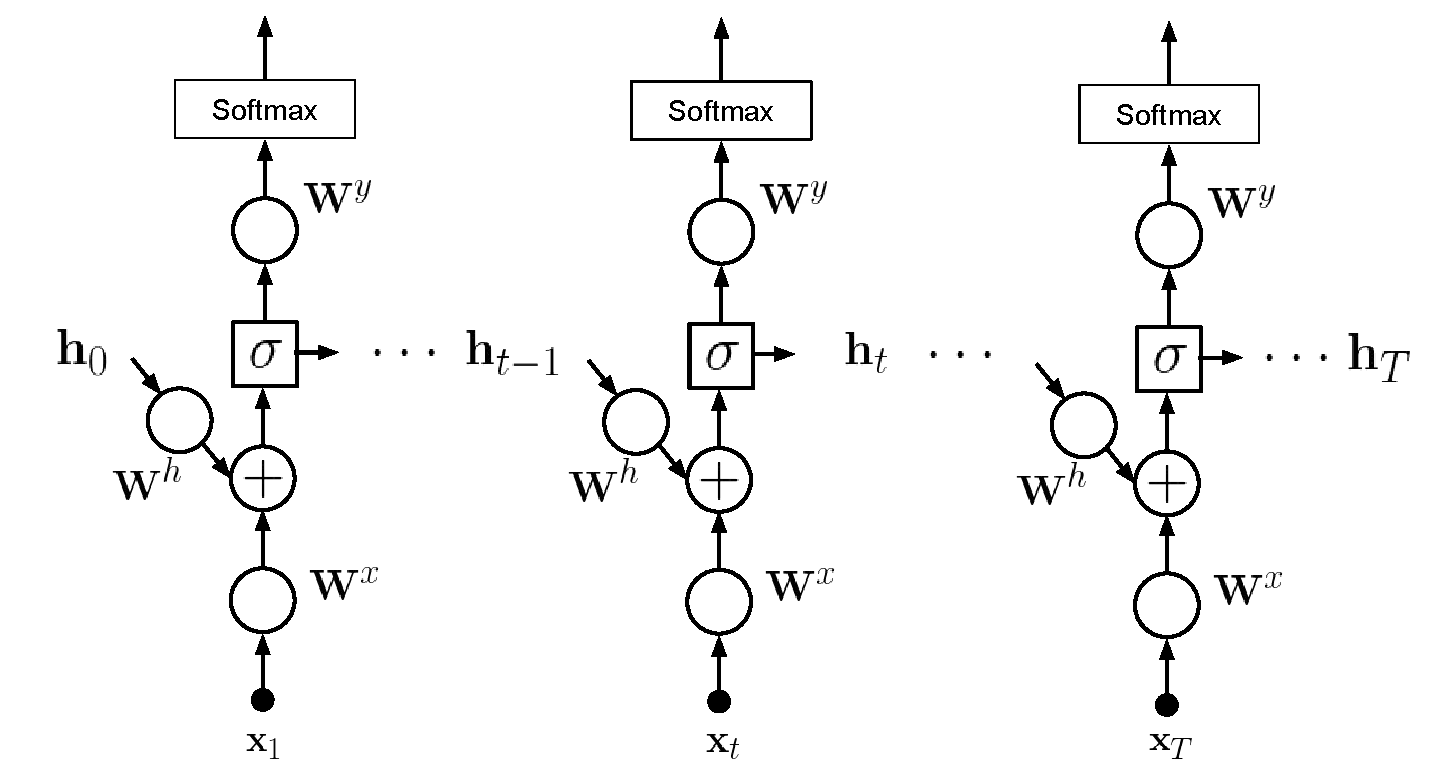
\includegraphics[scale=0.6]{figs/deep_learning/RNN.pdf}
\caption{The simplest RNN can be seen as replicating a single hidden-layer FF
network $T$ times and passing the intermediate hidden variable $\mathbf{h}_t$
across different steps. Note that all nodes operate over vector inputs e.g,.
$\mathbf{x}_t \in \mathbb{R}^I$. Circles indicate matrix multiplications.}
\label{fig:RNN}
\end{figure}

The previous day was focused Feed Forward (FF) networks. These networks are ill
suited to learn variable length patterns since they only accept inputs of a
fixed size. In order to learn sequences using neural networks, we need therefore
to define some architecture that is able to process variable length inputs.
Recurrent Neural Networks (RNNs) solve this problem by unfolding the
computation graph in time. In other words, the network is replicated as many
times as it is necessary to cover the sequence to be modeled. In order
to model the sequence one or more connections across different time instants are
created. This allows the network to have a memory in time and thus capture
complex patterns in sequences. In the simplest model, depicted in
Fig.~\ref{fig:RNN}, and detailed in Algorithm~\ref{algo:rnnforward}, a RNN is
created by replicating a single hidden-layer FF network $T$ times and passing
the intermediate hidden variable across different steps. 

Since RNNs are computation graphs involving the same operations as FF networks,
they can also be trained with back-propagation. However the error is
 propagated over the length of the entire sequence. This often leads to 
numerical problems know as \textit{vanishing} and \textit{exploding} gradients.
A number of solutions are used to mitigate this issue. One simple, yet inelegant,
method is clipping the gradients to a fixed threshold. Another solution is to resort to more complex 
RNN models that are able to better handle long range dependencies and are less
sensitive to this phenomena. It is important to bear in mind, however, that
all RNNs still use back-propagation as seen in the previous day, although it is
often referred as \textit{Back-propagation through time}. 

%What we saw with FF and RNN netwoeksThe only
%difference is that, as the complexity of the computation graph grows, it is
%increasingly difficult to derive individual closed form solutions for each model.
%This is the reason to resort to tools like Theano or TensorFlow, allow us
%to define arbitrary computation graphs and derive the gradients automatically.

\begin{algorithm}[th!]
\label{algo:rnnforward}
   \caption{Forward pass of a Recurrent Neural Network (RNN)}
\begin{algorithmic}[1]

   \STATE {\bfseries input:} Initial parameters for an RNN Input
$\Theta=\{\mathbf{W}^x \in \mathbb{R}^{H \times I}, \mathbf{W}^h \in \mathbb{R}^{H \times H}, \mathbf{W}^y \in \mathbb{R}^{K \times H} \}$ input, recurrent and output transformations respectively.

   \STATE {\bfseries input:} Input data matrix $\mathbf{x} \in \mathbb{R}^{I \times T}$ of size $T$. Initial recurrent variable $\mathbf{h}_0$. 

	\FOR{$t=1$ {\bfseries to} $T-1$}
     \STATE Apply linear transformation combining input and recurrent signals
        $$z_{jt}^h = \sum_{i=1}^{I} W_{ji}^x x_{it} + \sum_{j=1}^{J} W_{jj'}^h h_{j't-1}$$
     \STATE Apply non-linear transformation e.g. sigmoid (hereby denoted $\sigma()$)
     $$h_{jt} = \sigma(z_{jt}^h)  = \frac{1}{1+\exp(-z_{jt}^h)}$$

	\ENDFOR

\STATE Apply final linear transformation to each of the recurrent variables $\mathbf{h}_1 \cdots \mathbf{h}_T$ 
   $$z_{kt}^y = \sum_{j=1}^{J} W_{kj}^y h_{jt}$$
\STATE Apply final non-linear transformation e.g. softmax 
$$p(y_t=k|\mathbf{x}_{t:}) = \frac{\exp(z_{kt}^y)}{\sum_{k'=1}^{K} \exp(z_{k't}^y)}$$

\end{algorithmic}
\end{algorithm}

\begin{exercise}
Convince yourself that a RNN is just an FF unfolded in time. Run the NumpyRNN
code. Set break-points and compare with what you learned about back-propagation
in the previous day. 

To work with RNNs we will use the Part-of-speech data-set seen in the sequence
models day.
\begin{python}
# Load Part-of-Speech data 
import lxmls.readers.pos_corpus as pcc
corpus = pcc.PostagCorpus()
train_seq = corpus.read_sequence_list_conll("data/train-02-21.conll", max_sent_len=15, max_nr_sent=1000)
test_seq = corpus.read_sequence_list_conll("data/test-23.conll", max_sent_len=15, max_nr_sent=1000)
dev_seq = corpus.read_sequence_list_conll("data/dev-22.conll", max_sent_len=15, max_nr_sent=1000) 
\end{python}
We will need to redo the indices of
the data so that they are consecutive and cast all data to numpy arrays
of int32 for compatibility with GPUs. This function will also add reverse
indices to recover tag and word from its index word\_dict and tag\_dict  
\begin{python}
# Redo indices 
train_seq, test_seq, dev_seq = pcc.compacify(train_seq, test_seq, dev_seq, theano=True)
# Get number of words and tags in the corpus
nr_words = len(train_seq.x_dict)
nr_tags = len(train_seq.y_dict)
\end{python}

\noindent Load and configure the NumpyRNN. Remember to user reload if you want to modify 
the code inside the rnns module
\begin{python}
import lxmls.deep_learning.rnn as rnns
reload(rnns)
# RNN configuration
SEED = 1234       # Random seed to initialize weigths
emb_size = 50     # Size of word embeddings
hidden_size = 20  # size of hidden layer
# RNN
np_rnn = rnns.NumpyRNN(nr_words, emb_size, hidden_size, nr_tags, seed=SEED)
# Example sentence
x0 = train_seq[0].x
y0 = train_seq[0].y
\end{python}
Compute forward pass and gradients
\begin{python}
# Forward pass
p_y, y_rnn, h, z1, x = np_rnn.forward(x0, all_outputs=True)
# Gradients
numpy_rnn_gradients = np_rnn.grads(x0, y0)
\end{python}

\end{exercise}

\section{The Scan operation in Theano}

Handling variable length computation graphs in an automatic fashion is not simple. 
Theano provides the \textit{scan} function for this purpose. The scan function acts
as a symbolic for loop. Since, unlike for normal python for loops, it is not
possible to put a breakpoint in the scan loop, the design of graphs
with scan has to be handled with care. Toolboxes like Keras conveniently abstract
the user from such constructs. However, for complex designs it will be
necessary to be able to use scan or equivalent functions. 

\begin{exercise}
Understand the basics of scan with these examples. Scan allows you to build
computation graphs with a variable number of nodes. It acts as a python "for"
loop but it is symbolic. The following example should help you understand the
basic scan functionality. It generates a sequence for a given length. Run it
and modify it. Try to arrive at an error and understand whant happened.
\begin{python}
import numpy as np
import theano
import theano.tensor as T
theano.config.optimizer='None'

def square(x): 
    return x**2 

# Python
def np_square_n_steps(nr_steps):
    out = []
    for n in np.arange(nr_steps):
        out.append(square(n))
    return np.array(out)


\end{python}
\begin{python}
# Theano
nr_steps = T.lscalar('nr_steps')
h, _ = theano.scan(fn=square, sequences=T.arange(nr_steps))
th_square_n_steps = theano.function([nr_steps], h)

# Compare both
print np_square_n_steps(10)
print th_square_n_steps(10)
\end{python}
The following example should help you understand about matrix multiplications
and passing values from one iteration to the other. At each step, we will
multiply the output of the previous step by a matrix A. We start with an
initial vector s0. The matrix and vector are random but normalized to result on
a Markov chain (this is irrelevant for the use of scan).  
\begin{python}
# Configuration
nr_states = 3
nr_steps = 5

# Transition matrix
A = np.abs(np.random.randn(nr_states, nr_states))
A = A/A.sum(0, keepdims=True)
# Initial state
s0 = np.zeros(nr_states)
s0[0] = 1
\end{python}


\begin{python}
# Numpy version
def np_markov_step(s_tm1): 
    s_t = np.dot(s_tm1, A.T)
    return s_t 

def np_markov_chain(nr_steps, A, s0):
    # Pre-allocate space
    s = np.zeros((nr_steps+1, nr_states))
    s[0, :] = s0
    for t in np.arange(nr_steps):
        s[t+1, :] = np_markov_step(s[t, :])
    return  s   

np_markov_chain(nr_steps, A, s0)
\end{python}

\begin{python}
# Theano version
# Store variables as shared variables
th_A = theano.shared(A, name='A', borrow=True)
th_s0 = theano.shared(s0, name='s0', borrow=True)
# Symbolic variable for the number of steps
th_nr_steps = T.lscalar('nr_steps')

def th_markov_step(s_tm1): 
    s_t = T.dot(s_tm1, th_A.T)
    # Remember to name variables
    s_t.name = 's_t'
    return s_t 

s, _ = theano.scan(th_markov_step, 
                   outputs_info=[dict(initial=th_s0)], 
                   n_steps=th_nr_steps)
th_markov_chain = theano.function([th_nr_steps], T.concatenate((th_s0[None, :], s), 0))

th_markov_chain(nr_steps)
\end{python}
\end{exercise}

\section{A RNN in Theano for Part-of-Speech Tagging}

\begin{exercise}
Complete the theano code for a RNN inside lxmls/deep learning/rnn.py. Use
exercise 6.1 for a numpy example and 6.2 to learn how to handle scan. Keep in
mind that you only need to implement the forward pass! Theano will handle
backpropagation for us. 
\begin{python}
# Instantiate the class
rnn = rnns.RNN(nr_words, emb_size, hidden_size, nr_tags, seed=SEED)
# Compile the forward pass function
x = T.ivector('x')
th_forward = theano.function([x], rnn._forward(x).T)
\end{python}
When working with theano, it is more difficult to localize the source of
errors. It is therefore important to work step by step and test the
code frequently. To debug we suggest to implement and compile the forward pass
first. You can use this code for testing. If it raises no error you are good to
go.
\begin{python}
assert np.allclose(th_forward(x0), np_rnn.forward(x0)), \
    "Numpy and Theano forward pass differ!"
\end{python}
Once you are confident the forward pass is working you can test the gradients
\begin{python}
# Compile function returning the list of gradients
x = T.ivector('x')     # Input words
y = T.ivector('y')     # gold tags 
p_y = rnn._forward(x)
cost = -T.mean(T.log(p_y)[T.arange(y.shape[0]), y])
grads_fun = theano.function([x, y], [T.grad(cost, par) for par in rnn.param])
\end{python}

\begin{python}
# Compare numpy and theano gradients
theano_rnn_gradients = grads_fun(x0, y0)
for n in range(len(theano_rnn_gradients)): 
    assert np.allclose(numpy_rnn_gradients[n], theano_rnn_gradients[n]), \
        "Numpy and Theano gradients differ in step n"
\end{python}

\noindent Finally, its time to test our network in the task of POS tagging. Lets define
the optimization parameters and compile batch update and prediction
functions

%For this,
%lets first compile a function that does predictions
%\begin{python}
%rnn_prediction = theano.function([x], T.argmax(p_y, 1))
%# Lets test the predictions
%def test_model(sample_seq, rnn_prediction):
%    words = [train_seq.word_dict[wrd] for wrd in sample_seq.x]
%    tags = [train_seq.tag_dict[pred] for pred in rnn_prediction(sample_seq.x)]
%    print ["/".join([word, tag]) for word , tag in zip(words, tags)]
%\end{python}
\begin{python}
# Parameters
lrate = 0.5   # Learning rate
n_iter = 5    # Number of iterations
# Get list of SGD batch update rule for each parameter
updates = [(par, par - lrate*T.grad(cost, par)) for par in rnn.param]
# compile
rnn_prediction = theano.function([x], T.argmax(p_y, 1))
rnn_batch_update = theano.function([x, y], cost, updates=updates)
\end{python}

\clearpage

\noindent To train the newtwork with SGD, you can use the following code for
this purpose
\begin{python}
nr_words = sum([len(seq.x) for seq in train_seq])
for i in range(n_iter):
    # Training
    cost = 0
    errors = 0
    for n, seq in enumerate(train_seq):
        cost += rnn_batch_update(seq.x, seq.y)
        errors += sum(rnn_prediction(seq.x) != seq.y)
    acc_train = 100*(1-errors*1./nr_words) 
    print "Epoch %d: Train cost %2.2f Acc %2.2f %%" % (i+1, cost, acc_train), 
    # Evaluation    
    errors = 0
    for n, seq in enumerate(dev_seq):
        errors += sum(rnn_prediction(seq.x) != seq.y)  
    acc_dev = 100*(1-errors*1./nr_words) 
    print " Devel Acc %2.2f %%" % acc_dev
    sys.stdout.flush()
\end{python}


\end{exercise}


\section{The Importance of Pre-training}

% TODO: Maybe make this about Pre-raining and Dropout?

One of the key insights that has played a role in the rise of deep learning in
NLP tasks is the use of neural word-embeddings. These are just numeric 
representations of words that can be learned from unsupervised data using
simple FF networks such as e.g. skip-grams.

Such representations can be plugged into supervised models such as the RNN that we just
trained to initialize its initial layer. The use of pre-trained embeddings very often leads to
important improvements in performance. 

\begin{exercise}
Test the effect of using pre-trained embeddings. Run the following code to
download the embeddings. Reset the layer parameters and initialize the
embedding layer with the pre-trained embeddings. Then run the training code
from the last execise.
\begin{python}
# Embeddings Path
import lxmls.deep_learning.embeddings as emb
import os
reload(emb)
if not os.path.isfile(EMBEDDINGS):
    emb.download_embeddings('senna_50', "data/senna_50")
E = emb.extract_embeddings("data/senna_50", train_seq.x_dict) 
# Reset model to remove the effect of training
rnn = rnns.reset_model(rnn, seed=SEED)
# Set the embedding layer to the pre-trained values
rnn.param[0].set_value(E.astype(theano.config.floatX)) 

# Now re-run SGD training
\end{python}
\end{exercise}

\section{More Complex RNNs: LSTMs}

As previously mentioned, the basic RNN that we saw until now suffers from a
number of drawbacks like exploding or vanishing gradients, and the inability to
model long term dependencies. These deficiencies are solved by more complex
RNNs that include more complex internal logics, and are able to selectively
forget, thus capturing better long term information. The so called Long Short-Term Memory
(LSTM) and Gated Recurrent Unit (GRU) have replaced simple RNNs in most of modern
models. However, they only imply more complex architectures. For an excellent 
visual explanation of the differences between simples RNNs, GRUs and LSTMS please visit 

\begin{verbatim}
http://colah.github.io/posts/2015-08-Understanding-LSTMs/
\end{verbatim}

\begin{figure}[!h]
\centering
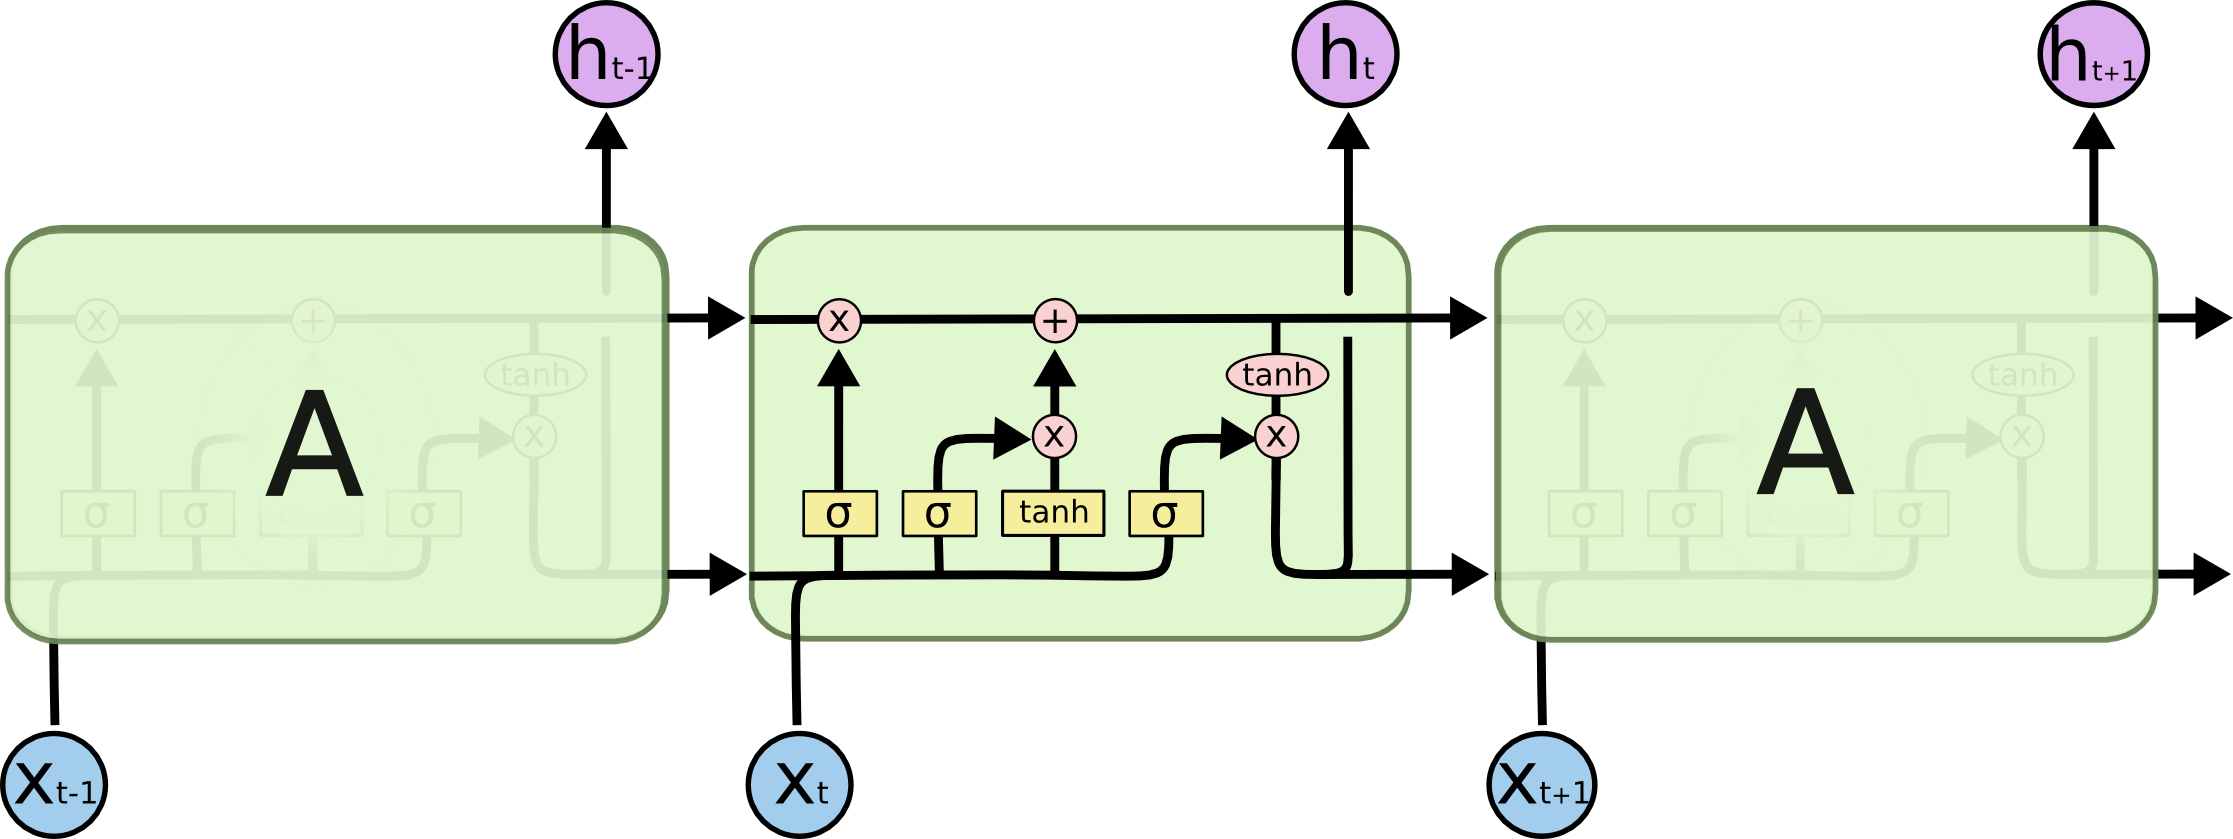
\includegraphics[scale=0.6]{figs/deep_learning/LSTM3-chain.png}
\caption{Detailed explanation of the LSTM internal logic, see source: \url{http://colah.github.io/posts/2015-08-Understanding-LSTMs/}.}
\label{fig:RNN}
\end{figure}

\begin{exercise}
Convince yourself that LSTMs are just more complex RNNs. Run them, play around
with the hyper parameters and compare the RNN and LSTM classes.
\begin{python}
# Instantiate LSTM
lstm = rnns.LSTM(nr_words, emb_size, hidden_size, nr_tags)
# Compile prediction and bacth update functions
lstm_prediction = theano.function([x], T.argmax(lstm._forward(x), 1))
lstm_cost = -T.mean(T.log(lstm._forward(x))[T.arange(y.shape[0]), y])
# Get list of SGD batch update rule for each parameter
lstm_updates = [(par, par - lrate*T.grad(lstm_cost, par)) for par in lstm.param]
# compile
lstm_batch_update = theano.function([x, y], lstm_cost, updates=lstm_updates)
\end{python}

\begin{python}
nr_words = sum([len(seq.x) for seq in train_seq])
for i in range(n_iter):
    # Training
    cost = 0
    errors = 0
    for n, seq in enumerate(train_seq):
        cost += lstm_batch_update(seq.x, seq.y)
        errors += sum(lstm_prediction(seq.x) != seq.y)
    acc_train = 100*(1-errors*1./nr_words) 
    print "Epoch %d: Train cost %2.2f Acc %2.2f %%" % (i+1, cost, acc_train), 
    # Evaluation:
    errors = 0
    for n, seq in enumerate(dev_seq):
        errors += sum(lstm_prediction(seq.x) != seq.y)  
    acc_dev = 100*(1-errors*1./nr_words) 
    print " Devel Acc %2.2f %%" % acc_dev
    sys.stdout.flush()
\end{python}
\end{exercise}


\chapter{Reinforcement Learning}
Today's class will introduce reinforcement learning. The previous classes
mainly focused on machine learning in a full supervision scenario, i.e., the
learning signal consisted of gold standard structures, and the learning goal
was to optimize the system parameters so as to maximize the likelihood of the
gold standard outputs.
    Reinforcement Learning (RL) assumes an \emph{interactive learning} scenario where a system learns by trial and error, using the consequences of its own actions to learn to maximize the expected reward from the environment.
    The learning scenario can also be seen as learning under \emph{weak supervision} in the sense that no gold standard examples are available, only rewards for system predictions.

\section{Today's assignment}

Your objective today should be to understand fully the concept of RL, including
the standard formalization of the environment as a Markov Decision Process
(MDP), and of the system as a stochastic policy. You will learn about
algorithms that evaluate the expected reward for a given policy (policy
evaluation/prediction) and algorithms that find the optimal policy parameters
(policy optimization/control). 

\section{Markov Decision Processes}

In order to define RL rigorously lets define an agent, for example a robot,
that is surrounded by an environment, for example a room full of objects. The
agent interacts with the environment in the following way: At each of a
sequence of time steps $t = 0,1,2,\ldots$,

\begin{itemize}
  \item the agent receives a \textbf{state} representation $S_t$,
  \item on which basis it selects an \textbf{action} $A_t$,
  \item and as a consequence, it receives a \textbf{reward} $R_{t+1}$,
  \item after which it finds itself in a new state $S_{t+1}$.
\end{itemize}

The Goal of RL is then to teach the agent to maximize the total amount of
reward it receives in such interactions in the long run. The standard
formalization of the environment is given by a \textbf{Markov Decision Process
(MDP)}, defined as a tuple $\left< \mathcal{S}, \mathcal{A}, \mathcal{P},
\mathcal{R} \right>$ where

  \begin{itemize}
  \item $\mathcal{S}$ is a set of states,
  \item $\mathcal{A}$ is a finite set of actions,
  \item $\mathcal{P}$ is a state transition probability matrix s.t. $\mathcal{P}_{ss'}^{a} = P[S_{t+1} = s' | S_t = s, A_t = a]$, 
  \item $\mathcal{R}$ is a reward function  s.t. $\mathcal{R}_s^a = \mathbb{E}[R_{t+1}| S_t = s, A_t = a]$. 
  \end{itemize}

% RAMON: Can we explain why the reward is given by an expectation at this point?

\section{Policies and Rewards}

The system is formalized as a \textbf{stochastic policy}, which is defined as a
distribution over actions given states s.t. $\pi(a|s) = P[A_t = a| S_t = s]$.
The two central tasks in RL consist of policy evaluation (a.k.a. prediction),
i.e., evaluation of the expected reward for a given policy; and policy
optimization (a.k.a. learning/control), i.e., finding the optimal policy under
the expected reward criterion. The reward criterion is formalized using the
concepts of \emph{return} and \emph{value functions}: 

\noindent The \textbf{total discounted return} from time-step $t$ for discount $\gamma \in [0,1]$ is

\begin{equation}
    G_t = R_{t+1} + \gamma R_{t+2} + \gamma^2 R_{t+3} + \ldots = \sum_{k=0}^{\infty}\gamma^k R_{t+k+1}.
\end{equation}

The \textbf{action-value function} $q_{\pi}(s,a)$ on an MDP is the expected return starting from state $s$, taking action $a$, and following policy $\pi$ s.t.

\begin{equation}
   q_{\pi}(s,a) = \mathbb{E}_{\pi}[G_t | S_t = s, A_t = a].
\end{equation}

The \textbf{state-value function} $v_{\pi}(s)$ of an MDP is the expected return starting from state $s$ and following policy $\pi$ s.t.

\begin{equation}
    v_{\pi}(s) = \mathbb{E}_{\pi}[G_t | S_t = s] = \mathbb{E}_{a \sim \pi}[q_{\pi}(s,a)] .
\end{equation}

% RAMON: Adding less mathematical, more intuitive explanations about the concepts above would help IMO    
    
\section{Dynamic Programming Solutions}

\begin{figure}[!ht]
\centering
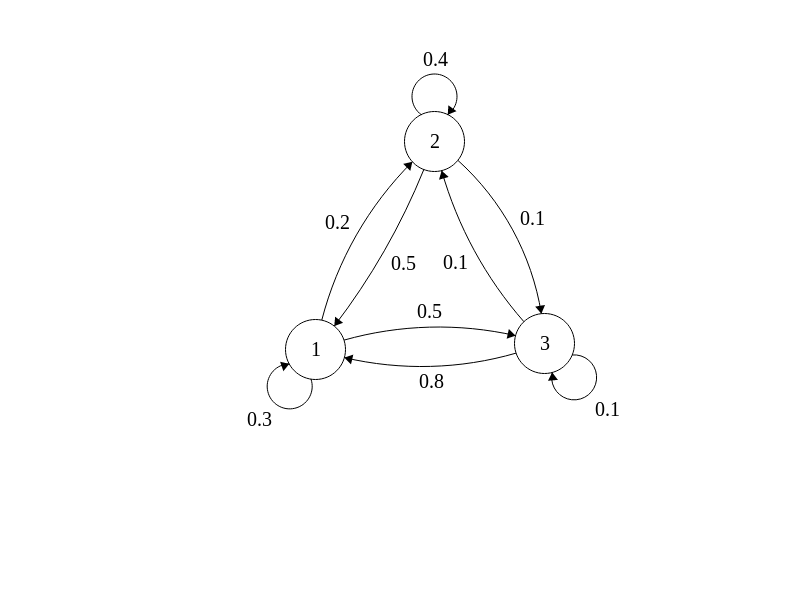
\includegraphics[scale=0.5,trim={0 5cm 0 1cm},clip]{figs/reinforcement_learning/mdp.png}
\caption{Markov Decision Process (MDP) with three states $\mathcal{S}=\{s_1,s_2,s_3\}$ and three possible actions $\mathcal{A}=\{a_1,a_2,a_3\}$, moving to state $s_1$, moving to state $s_2$ and moving to state $s_3$.}
\label{fig:MDP}
\end{figure}

Consider the (simplified) MDP represented in Figure \ref{fig:MDP}: it consists of three states (1, 2, and 3) that are connected by three actions (move to state 1, 2, or 3) that determine state transitions (our MDP is thus actually a Markov Reward Process (MRP) with deterministic state transitions). The rewards are 10.0, 2.0, and 3.0 for a transition into state 1, 2, and 3, respectively. 

Given full information about states and rewards, we want to evaluate a given policy. A central tool is the \textbf{Bellman Expectation Equation}, which tells us how to decompose the state-value function into immediate reward plus discounted value of successor state s.t.
\begin{align*}
    v_{\pi}(s) & = \mathbb{E}_{\pi}[R_{t+1} + \gamma v_{\pi}(S_{t+1}) | S_t = s]\\
    & = \sum_{a \in \mathcal{A}} \pi(a|s) \left( \mathcal{R}_s^a + \gamma \sum_{s' \in \mathcal{S}} \mathcal{P}_{ss'}^a v_{\pi}(s') \right).
\end{align*}

\noindent A straightforward solution is to solve the linear equation directly:
\begin{align*}
    \boldsymbol{v}_{\pi} & = (\boldsymbol{I} -  \gamma \boldsymbol{\mathcal{P}}^{\pi})^{-1} \boldsymbol{\mathcal{R}}^{\pi}.
\end{align*}
Because of the complexity of matrix inversion, this solution is applicable only to small MDPs. For larger MDPs, we can use iterative policy evaluation on the Bellman Expectation Equation.

\begin{exercise}
\label{exercise:PolicyEvaluation}
Implement policy evaluation by dynamic programming and linear programming. Check that you obtain the same value.

\begin{python}
import numpy as np

policy=np.array([[0.3, 0.2, 0.5], [0.5, 0.4, 0.1], [0.8, 0.1, 0.1]])
rewards=np.array([10., 2., 3.])

state_value_function=np.array([0 for i in range(3)])

for i in range(20):
    print(state_value_function)
    state_value_function=# TODO: Implement the Policy Evaluation Update with a Learning Rate of 0.1
print(state_value_function)

solution=# TODO: Implement the linear programming solution
print(solution)
\end{python}
\end{exercise}

\section{Monte Carlo and Q-Learning Solutions}

While Dynamic Programming techniques allow to iteratively compute policy evaluation and optimization problems, a disadvantage of these techniques is the fact that we need to know a full MDP model and touch all transitions and rewards in learning. Monte Carlo techniques circumvent this problem by learning from episodes that are sampled under a given policy. An algorithm for Monte Carlo Policy Evaluation looks as follows: 
\begin{itemize}
  \item Sample episodes $S_0, A_0, R_1, \ldots, R_T \sim \pi$.
    \item For each sampled episode:
  \begin{itemize}
  \item Increment state counter $N(s) \leftarrow N(s) + 1$.
  \item Increment total return $S(s) \leftarrow S(s) + G_t$.
    \end{itemize}
  \item Estimate mean return $V(s) = S(s)/N(s)$.
  \end{itemize}

A more sophisticated technique is the so-called Q-Learning algorithm. In contrast to the simple Monte Carlo Policy Evaluation algorithm given above, it updates not towards the actual return $G_t$, but towards an estimate $(R_{t+1} + \gamma \max_{a'} Q(S_{t+1},a')$ (the so-called Temporal Difference (TD) target). It thus combines Dynamic Programming (in form of the Bellman Optimality Equation) and Monte Carlo (by sampling episodes).

\begin{algorithm}[h!]
\label{algo:q-learning}
   \caption{Q-Learning}
\begin{algorithmic}[1]
\FOR{sampled episodes}
\STATE Initialize $S_t$
\FOR{steps $t$} 
\STATE Sample $A_t$, observe $R_{t+1}$, $S_{t+1}$.
\STATE $Q(S_t,A_t) \leftarrow (1 - \alpha) Q(S_t,A_t) + \alpha (R_{t+1} + \gamma \max_{a'} Q(S_{t+1},a'))$
\STATE $S_t \leftarrow S_{t+1}$.
\ENDFOR
	\ENDFOR
\end{algorithmic}
\end{algorithm}

\begin{exercise}
Implement Monte Carlo policy evaluation. See how similar results can be
obtained by using sampling
\begin{python}
import numpy as np

policy=np.array([[0.3, 0.2, 0.5], [0.5, 0.4, 0.1], [0.8, 0.1, 0.1]])
rewards=np.array([10., 2., 3.])

import random
from collections import defaultdict
reward_counter=np.array([0., 0., 0.])
visit_counter=np.array([0., 0., 0.])

def gt(rewardlist, gamma=0.1):
    '''
    Function to calculate the total discounted reward
    >>> gt([10, 2, 3], gamma=0.1)
    10.23
    '''
    #TODO: Implement the total discounted reward
    return 0

for i in range(400):
    start_state=random.randint(0, 2)
    next_state=start_state
    rewardlist=[]
    occurence=defaultdict(list) 
    for i in range(250):
        rewardlist.append(rewards[next_state]) 
        occurence[next_state].append(len(rewardlist)-1) 
        action=np.random.choice(np.arange(0, 3), p=policy[next_state]) 
        next_state=action

    for state in occurence: 
        for value in occurence[state]: 
            rew=gt(rewardlist[value:]) 
            reward_counter[state]+=rew 
            visit_counter[state]+=1 
            #break #if break: return following only the first visit

print(reward_counter/visit_counter)
\end{python}

Implement Q-Learning policiy optimization in a simple exercise. This samples a state-action pair randomly, so that all the state-action pairs can be seen.
\begin{python}
q_table=np.zeros((3, 3)) 
for i in range(1001): 
    state=random.randint(0, 2) 
    action=random.randint(0, 2) 
    next_state=action
    reward=rewards[next_state] 
    next_q=max(q_table[next_state])
    q_table[state, action]= #TODO: Implement the Q-Table update
    if i%100==0:
        print(q_table)
\end{python}
\end{exercise}


\section{Policy Gradient Techniques}

The Dynamic Programming and Monte Carlo techniques discussed above can be summarized under the header of \emph{value-based} techniques since they focus on value functions. They are thus inherently indirect. Direct solutions to policy optimization that use gradient-based techniques to optimize parametric (stochastic) policies are called \emph{policy gradient} techniques. Given an action-value function $q_{\pi_\theta}(S_t,A_t)$, the objective is to maximize the expected value  \[\mathbb{E}_{\pi_{\theta}}[q_{\pi_\theta}(S_t,A_t)].\]
The gradient of this objective is  
\[\mathbb{E}_{\pi_{\theta}}[q_{\pi_\theta}(S_t,A_t) \nabla_{\theta} \log \pi_{\theta}(A_t|S_t)].\]
The well-known REINFORCE algorithm optimizes this objective by using stochastic gradient ascent updates and by replacing $q_{\pi_\theta}(S_t,A_t)$ by the actual return $G_t$.

\begin{algorithm}[t!]
\label{algo:reinforce}
   \caption{REINFORCE}
\begin{algorithmic}[1]
\FOR{sampled episodes $y=S_0, A_0, R_1, \ldots, R_T \sim \pi_\theta$}
\FOR{time steps $t$} 
\STATE Obtain reward $G_t$%$q_{\pi_\theta}(S_t,A_t)$
\STATE Update $\theta \leftarrow \theta + \alpha (
G_t
%q_{\pi_\theta}(S_t,A_t) 
\nabla_{\theta} \log \pi_{\theta}(A_t|S_t))$
\ENDFOR
	\ENDFOR
\end{algorithmic}
\end{algorithm}



\begin{exercise}
Implement the score function gradient estimator in lxmls/reinforcement\_learning/score\_function\_estimator.py. Check it is correct by calling the train() function.
\begin{python}
\% matplotlib inline
from lxmls.reinforcement_learning.score_function_estimator import train
train()
\end{python}
\end{exercise}

A last exercise is to apply REINFORCE to the cart pole task: A pole is attached by an un-actuated joint to a cart, which moves along a frictionless track. The system is controlled by applying a force of +1 or -1 to the cart. The pendulum starts upright, and the goal is to prevent it from falling over. A reward of +1 is provided for every timestep that the pole remains upright. The episode ends when the pole is more than 15 degrees from vertical, or the cart moves more than 2.4 units from the center. See \url{ https://gym.openai.com/envs/CartPole-v1/}.

\begin{exercise}
Implement policy gradient for the cartpole task by coding the forward pass of Model() in lxmls/reinforcement\_learning/policy\_gradient.py. Check it is correct by calling the train() function.
\begin{python}
from lxmls.reinforcement_learning.policy_gradient import train
train()
\end{python}
\end{exercise}


\begin{exercise}
As a last exercise, apply what you have learned to the RNN model seen in previous days. Implement REINFORCE to replace the maximum likelihood loss used on the RNN day. For this you can modify the PolicyRNN class in lxmls/deep\_learning/pytorch\_models/rnn.py 
\begin{python}
# Load Part-of-Speech data 
from lxmls.readers.pos_corpus import PostagCorpusData
data = PostagCorpusData()

# Get batch iterators for train and test
batch_size = 1
train_batches = data.batches('train', batch_size=batch_size)
dev_set = data.batches('dev', batch_size=batch_size)
test_set = data.batches('test', batch_size=batch_size)
\end{python}
\begin{python}
reinforce = True

# Load version of the RNN 
from lxmls.deep_learning.pytorch_models.rnn import PolicyRNN
model = PolicyRNN(
    input_size=data.input_size,
    embedding_size=50,
    hidden_size=100,
    output_size=data.output_size,
    learning_rate=0.05,
    gamma=0.8,
    RL=reinforce,
    maxL=data.maxL
)
\end{python}

After finishing the implementation, the following code shoul run
\begin{python}
import numpy as np
import time

# Run training
num_epochs = 15

batch_size = 1
# Get batch iterators for train and test
train_batches = data.sample('train', batch_size=batch_size)
dev_set = data.sample('dev', batch_size=batch_size)
test_set = data.sample('test', batch_size=batch_size)

# Epoch loop
start = time.time()
for epoch in range(num_epochs):
    # Batch loop
    for batch in train_batches:
        model.update(input=batch['input'], output=batch['output'])
    # Evaluation dev
    is_hit = []
    for batch in dev_set:
        loss = model.predict_loss(batch['input'], batch['output'])
        is_hit.extend(loss)
    accuracy = 100 * np.mean(is_hit)
    # Inform user
    print("Epoch %d: dev accuracy %2.2f %%" % (epoch + 1, accuracy))

print("Training took %2.2f seconds per epoch" % ((time.time() - start) / num_epochs))
# Evaluation test
is_hit = []
for batch in test_set:
    is_hit.extend(model.predict_loss(batch['input'],batch['output']))
accuracy = 100 * np.mean(is_hit)

# Inform user
print("Test accuracy %2.2f %%" % accuracy)
\end{python}
\end{exercise}


% \appendix

% \chapter{Installation Guide}
% Installation instructions......
% \chapter{Data Sets}
% \section{\label{data:simple} Simple Dataset}

Explain, show the interface etc

\section{\label{data:amazon}Amazon review data set}

\section{\label{data:ptb} Penn TreeBank}


\section{\label{data:floresta} Floresta Sintáctica}




%\bibliographystyle{plain}
\bibliographystyle{apalike}
\bibliography{guide}
\end{document}
%%% Local Variables: 
%%% mode: latex
%%% TeX-master: t
%%% End: 
